\documentclass[twoside]{book}

% Packages required by doxygen
\usepackage{fixltx2e}
\usepackage{calc}
\usepackage{doxygen}
\usepackage[export]{adjustbox} % also loads graphicx
\usepackage{graphicx}
\usepackage[utf8]{inputenc}
\usepackage{makeidx}
\usepackage{multicol}
\usepackage{multirow}
\PassOptionsToPackage{warn}{textcomp}
\usepackage{textcomp}
\usepackage[nointegrals]{wasysym}
\usepackage[table]{xcolor}

% Font selection
\usepackage[T1]{fontenc}
\usepackage[scaled=.90]{helvet}
\usepackage{courier}
\usepackage{amssymb}
\usepackage{sectsty}
\renewcommand{\familydefault}{\sfdefault}
\allsectionsfont{%
  \fontseries{bc}\selectfont%
  \color{darkgray}%
}
\renewcommand{\DoxyLabelFont}{%
  \fontseries{bc}\selectfont%
  \color{darkgray}%
}
\newcommand{\+}{\discretionary{\mbox{\scriptsize$\hookleftarrow$}}{}{}}

% Page & text layout
\usepackage{geometry}
\geometry{%
  a4paper,%
  top=2.5cm,%
  bottom=2.5cm,%
  left=2.5cm,%
  right=2.5cm%
}
\tolerance=750
\hfuzz=15pt
\hbadness=750
\setlength{\emergencystretch}{15pt}
\setlength{\parindent}{0cm}
\setlength{\parskip}{0.2cm}
\makeatletter
\renewcommand{\paragraph}{%
  \@startsection{paragraph}{4}{0ex}{-1.0ex}{1.0ex}{%
    \normalfont\normalsize\bfseries\SS@parafont%
  }%
}
\renewcommand{\subparagraph}{%
  \@startsection{subparagraph}{5}{0ex}{-1.0ex}{1.0ex}{%
    \normalfont\normalsize\bfseries\SS@subparafont%
  }%
}
\makeatother

% Headers & footers
\usepackage{fancyhdr}
\pagestyle{fancyplain}
\fancyhead[LE]{\fancyplain{}{\bfseries\thepage}}
\fancyhead[CE]{\fancyplain{}{}}
\fancyhead[RE]{\fancyplain{}{\bfseries\leftmark}}
\fancyhead[LO]{\fancyplain{}{\bfseries\rightmark}}
\fancyhead[CO]{\fancyplain{}{}}
\fancyhead[RO]{\fancyplain{}{\bfseries\thepage}}
\fancyfoot[LE]{\fancyplain{}{}}
\fancyfoot[CE]{\fancyplain{}{}}
\fancyfoot[RE]{\fancyplain{}{\bfseries\scriptsize Generated on Thu Sep 24 2015 12\+:49\+:13 for 3\+D\+B\+G\+B by Doxygen }}
\fancyfoot[LO]{\fancyplain{}{\bfseries\scriptsize Generated on Thu Sep 24 2015 12\+:49\+:13 for 3\+D\+B\+G\+B by Doxygen }}
\fancyfoot[CO]{\fancyplain{}{}}
\fancyfoot[RO]{\fancyplain{}{}}
\renewcommand{\footrulewidth}{0.4pt}
\renewcommand{\chaptermark}[1]{%
  \markboth{#1}{}%
}
\renewcommand{\sectionmark}[1]{%
  \markright{\thesection\ #1}%
}

% Indices & bibliography
\usepackage{natbib}
\usepackage[titles]{tocloft}
\setcounter{tocdepth}{3}
\setcounter{secnumdepth}{5}
\makeindex

% Hyperlinks (required, but should be loaded last)
\usepackage{ifpdf}
\ifpdf
  \usepackage[pdftex,pagebackref=true]{hyperref}
\else
  \usepackage[ps2pdf,pagebackref=true]{hyperref}
\fi
\hypersetup{%
  colorlinks=true,%
  linkcolor=blue,%
  citecolor=blue,%
  unicode%
}

% Custom commands
\newcommand{\clearemptydoublepage}{%
  \newpage{\pagestyle{empty}\cleardoublepage}%
}


%===== C O N T E N T S =====

\begin{document}

% Titlepage & ToC
\hypersetup{pageanchor=false,
             bookmarks=true,
             bookmarksnumbered=true,
             pdfencoding=unicode
            }
\pagenumbering{roman}
\begin{titlepage}
\vspace*{7cm}
\begin{center}%
{\Large 3\+D\+B\+G\+B \\[1ex]\large 1.\+3 }\\
\vspace*{1cm}
{\large Generated by Doxygen 1.8.10}\\
\vspace*{0.5cm}
{\small Thu Sep 24 2015 12:49:13}\\
\end{center}
\end{titlepage}
\clearemptydoublepage
\tableofcontents
\clearemptydoublepage
\pagenumbering{arabic}
\hypersetup{pageanchor=true}

%--- Begin generated contents ---
\chapter{Modules Index}
\section{Modules List}
Here is a list of all modules with brief descriptions\+:\begin{DoxyCompactList}
\item\contentsline{section}{\hyperlink{namespaceglobvar}{globvar} }{\pageref{namespaceglobvar}}{}
\item\contentsline{section}{\hyperlink{namespacegridvar}{gridvar} }{\pageref{namespacegridvar}}{}
\end{DoxyCompactList}

\chapter{File Index}
\section{File List}
Here is a list of all files with brief descriptions\+:\begin{DoxyCompactList}
\item\contentsline{section}{C\+:/\+Git3\+D\+B\+G\+B/source/\hyperlink{_8__lspfit_8f}{.\+\_\+lspfit.\+f} }{\pageref{_8__lspfit_8f}}{}
\item\contentsline{section}{C\+:/\+Git3\+D\+B\+G\+B/source/\hyperlink{3dbgb_8f90}{3dbgb.\+f90} }{\pageref{3dbgb_8f90}}{}
\item\contentsline{section}{C\+:/\+Git3\+D\+B\+G\+B/source/\hyperlink{airfoiltypes_8f90}{airfoiltypes.\+f90} }{\pageref{airfoiltypes_8f90}}{}
\item\contentsline{section}{C\+:/\+Git3\+D\+B\+G\+B/source/\hyperlink{b3d2sec_8f90}{b3d2sec.\+f90} }{\pageref{b3d2sec_8f90}}{}
\item\contentsline{section}{C\+:/\+Git3\+D\+B\+G\+B/source/\hyperlink{bladegen_8f90}{bladegen.\+f90} }{\pageref{bladegen_8f90}}{}
\item\contentsline{section}{C\+:/\+Git3\+D\+B\+G\+B/source/\hyperlink{bladegrid2_d_8f90}{bladegrid2\+D.\+f90} }{\pageref{bladegrid2_d_8f90}}{}
\item\contentsline{section}{C\+:/\+Git3\+D\+B\+G\+B/source/\hyperlink{bladestack_8f90}{bladestack.\+f90} }{\pageref{bladestack_8f90}}{}
\item\contentsline{section}{C\+:/\+Git3\+D\+B\+G\+B/source/\hyperlink{bspline3_8f90}{bspline3.\+f90} }{\pageref{bspline3_8f90}}{}
\item\contentsline{section}{C\+:/\+Git3\+D\+B\+G\+B/source/\hyperlink{bsplinecam_8f90}{bsplinecam.\+f90} }{\pageref{bsplinecam_8f90}}{}
\item\contentsline{section}{C\+:/\+Git3\+D\+B\+G\+B/source/\hyperlink{cubicspline_8f90}{cubicspline.\+f90} }{\pageref{cubicspline_8f90}}{}
\item\contentsline{section}{C\+:/\+Git3\+D\+B\+G\+B/source/\hyperlink{dmat__solve_8f90}{dmat\+\_\+solve.\+f90} }{\pageref{dmat__solve_8f90}}{}
\item\contentsline{section}{C\+:/\+Git3\+D\+B\+G\+B/source/\hyperlink{ellipgrid_8f90}{ellipgrid.\+f90} }{\pageref{ellipgrid_8f90}}{}
\item\contentsline{section}{C\+:/\+Git3\+D\+B\+G\+B/source/\hyperlink{errors_8f90}{errors.\+f90} }{\pageref{errors_8f90}}{}
\item\contentsline{section}{C\+:/\+Git3\+D\+B\+G\+B/source/\hyperlink{func_nsubs_8f90}{func\+Nsubs.\+f90} }{\pageref{func_nsubs_8f90}}{}
\item\contentsline{section}{C\+:/\+Git3\+D\+B\+G\+B/source/\hyperlink{globvar_8f90}{globvar.\+f90} }{\pageref{globvar_8f90}}{}
\item\contentsline{section}{C\+:/\+Git3\+D\+B\+G\+B/source/\hyperlink{lespline_8f90}{lespline.\+f90} }{\pageref{lespline_8f90}}{}
\item\contentsline{section}{C\+:/\+Git3\+D\+B\+G\+B/source/\hyperlink{lesting_8f90}{lesting.\+f90} }{\pageref{lesting_8f90}}{}
\item\contentsline{section}{C\+:/\+Git3\+D\+B\+G\+B/source/\hyperlink{lspfit_8f}{lspfit.\+f} }{\pageref{lspfit_8f}}{}
\item\contentsline{section}{C\+:/\+Git3\+D\+B\+G\+B/source/\hyperlink{readinput_8f90}{readinput.\+f90} }{\pageref{readinput_8f90}}{}
\item\contentsline{section}{C\+:/\+Git3\+D\+B\+G\+B/source/\hyperlink{spanwise__output_8f90}{spanwise\+\_\+output.\+f90} }{\pageref{spanwise__output_8f90}}{}
\item\contentsline{section}{C\+:/\+Git3\+D\+B\+G\+B/source/\hyperlink{spanwise__variation_8f90}{spanwise\+\_\+variation.\+f90} }{\pageref{spanwise__variation_8f90}}{}
\item\contentsline{section}{C\+:/\+Git3\+D\+B\+G\+B/source/\hyperlink{spline_8f90}{spline.\+f90} }{\pageref{spline_8f90}}{}
\item\contentsline{section}{C\+:/\+Git3\+D\+B\+G\+B/source/\hyperlink{splinethick_8f90}{splinethick.\+f90} }{\pageref{splinethick_8f90}}{}
\item\contentsline{section}{C\+:/\+Git3\+D\+B\+G\+B/source/\hyperlink{techop_8f90}{techop.\+f90} }{\pageref{techop_8f90}}{}
\end{DoxyCompactList}

\chapter{Module Documentation}
\hypertarget{namespaceglobvar}{}\section{globvar Module Reference}
\label{namespaceglobvar}\index{globvar@{globvar}}
\subsection*{Variables}
\begin{DoxyCompactItemize}
\item 
integer \hyperlink{namespaceglobvar_a074233db9e9693042a79a9e4cd4f84e2}{ibrow}
\item 
integer \hyperlink{namespaceglobvar_aefeb81e8846810feb44bb79f95cac5c2}{ile}
\item 
integer \hyperlink{namespaceglobvar_a67308a23e61fb67077fcb6216e72bc84}{ite}
\item 
integer \hyperlink{namespaceglobvar_aa6b683519cf0d2993847908919dd2d72}{j}
\item 
integer \hyperlink{namespaceglobvar_ab47e00ad68c86a9aac86e082da7398f1}{ledegree}
\item 
integer \hyperlink{namespaceglobvar_a64988ba2eed57cebc3d95939e33ee75e}{no\+\_\+le\+\_\+segments}
\item 
integer \hyperlink{namespaceglobvar_a5c850302345bc4b2d45af2d4bb80f58f}{csng}
\item 
character $\ast$256 \hyperlink{namespaceglobvar_a91c6656f75994719c2ef6ca7d7b88ded}{fext}
\item 
character $\ast$256 \hyperlink{namespaceglobvar_a1620db6ffc17c057934b90f70421dd96}{line2}
\item 
character $\ast$256 \hyperlink{namespaceglobvar_a3ee916788a2f55473d7d6dd7ba5137f7}{argp1}
\item 
character $\ast$256 \hyperlink{namespaceglobvar_a61ebbf94ac2ff67042612526d08b69f5}{ok}
\item 
character $\ast$16 \hyperlink{namespaceglobvar_ae058016a63919ba09dda0290e83e60a0}{blrow}
\item 
character $\ast$16 \hyperlink{namespaceglobvar_a62eb55ad192fba73ef6d49482206212e}{radialsec}
\item 
character $\ast$32, dimension(100) \hyperlink{namespaceglobvar_afebc24dd143d18989fbeb7223a277ab8}{blext}
\item 
character $\ast$32 \hyperlink{namespaceglobvar_a0a6c526cbc0a41ebd6f3667a0a9183ba}{casename}
\item 
character $\ast$32 \hyperlink{namespaceglobvar_a6a1dfe25b49d1fa165e1f63466b92629}{spanwise\+\_\+spline}
\item 
character $\ast$256 \hyperlink{namespaceglobvar_a35d25dc36b9abbf2f578dcdb231ba86d}{anglespline}
\item 
character $\ast$10 \hyperlink{namespaceglobvar_a893ea8284df7ea110ea93d673cf237f9}{ibrowc}
\item 
character $\ast$10 \hyperlink{namespaceglobvar_a0a7f8083468e94d2d3aae1f309fb2dd4}{ibrowc1}
\item 
character $\ast$20, dimension(100) \hyperlink{namespaceglobvar_ae69735f940091c76c32c20b4cd90ebb4}{airfoil}
\item 
character $\ast$20, dimension(\+:), allocatable \hyperlink{namespaceglobvar_a8e9e3ba0b38e35c9b6b0c02e62ffc1f8}{throat\+\_\+pos}
\item 
character $\ast$32 \hyperlink{namespaceglobvar_acc5999ee5e843ad4d03a5047a316e813}{develop}
\item 
character $\ast$32 \hyperlink{namespaceglobvar_a32441db96414a17de3451c8789d1edb3}{xygrid}
\item 
character $\ast$32 \hyperlink{namespaceglobvar_a683af9844336d830d4c99a6f542260ad}{xyzstreamlines}
\item 
character $\ast$80 \hyperlink{namespaceglobvar_a914ee6e2252c7098aff0eb09f1646f79}{file1}
\item 
character $\ast$80 \hyperlink{namespaceglobvar_a95f5c32d6cc281292091a3f0c77928e2}{file2}
\item 
character $\ast$80 \hyperlink{namespaceglobvar_a50a9cac1bfd7e2b8ba993f2e494e61af}{file3}
\item 
character $\ast$80 \hyperlink{namespaceglobvar_ad37b1da3092de9a9a76be4f2f8c97231}{file4}
\item 
character $\ast$80 \hyperlink{namespaceglobvar_a2cf5ea09c434891e0a0154c05a3a55dc}{file5}
\item 
character $\ast$80 \hyperlink{namespaceglobvar_a1f007a363d48ae7b896f7303fb7b94c9}{file6}
\item 
character $\ast$80 \hyperlink{namespaceglobvar_aedb6df66bd85d51a0e7a4abaf0833074}{file7}
\item 
character $\ast$80 \hyperlink{namespaceglobvar_afe69a24b80357a46880b963d07e777f4}{file8}
\item 
character $\ast$80 \hyperlink{namespaceglobvar_ae35b72b87d0bb3063a6a44013250ce2a}{file9}
\item 
character $\ast$80 \hyperlink{namespaceglobvar_a6581bd3170639009e3b516cfef2969cf}{file10}
\item 
character $\ast$80 \hyperlink{namespaceglobvar_a8150c7754f44712fdeb69767f63ac557}{file11}
\item 
character(len=2) \hyperlink{namespaceglobvar_a5a48d5b0df94151f6ccff35f89d832ed}{units}
\item 
character(len=1) \hyperlink{namespaceglobvar_a113718364777f5700503cc4655ea8a36}{trueleansweep}
\item 
integer \hyperlink{namespaceglobvar_ad587987756a26ab8482d669091aa11e2}{f1}
\item 
integer \hyperlink{namespaceglobvar_ab013958d5d057b8aca4e06ba0daa8406}{f2}
\item 
integer \hyperlink{namespaceglobvar_a22ec31cd077818915aa449475242ebc1}{f3}
\item 
integer \hyperlink{namespaceglobvar_ac3c062c849a3ecf6de129ae085a265ae}{f4}
\item 
integer \hyperlink{namespaceglobvar_aef4e41982e8eb0e0436d5261df60a5ba}{f5}
\item 
integer \hyperlink{namespaceglobvar_a9bcf733cb3d2746a17a750550de00730}{f6}
\item 
integer \hyperlink{namespaceglobvar_ad5518ff994222c6d414b1ab14ec5ff3b}{f7}
\item 
integer \hyperlink{namespaceglobvar_a81a49408c447c53cabc16ec197a0520f}{f8}
\item 
integer \hyperlink{namespaceglobvar_ae5c9f355184c5007c6fd6e3e77ff5006}{f9}
\item 
integer \hyperlink{namespaceglobvar_a31893a074cdc83965ae93c821376be2b}{f10}
\item 
integer \hyperlink{namespaceglobvar_a8107e26d71f5d153179d812a2060f289}{f11}
\item 
integer \hyperlink{namespaceglobvar_a9b05c54fac739f587c870e529b2216f9}{i}
\item 
integer \hyperlink{namespaceglobvar_a0f5c9c2384e0fd1c79c5e07df615661f}{js}
\item 
integer \hyperlink{namespaceglobvar_ac3085057e6f2d3302a5046006457c547}{k}
\item 
integer \hyperlink{namespaceglobvar_ae7c4dc9c253893de2f413b45f223f1a9}{p}
\item 
integer \hyperlink{namespaceglobvar_a4bcc489e884542bc5eb30f17d5773278}{nsec}
\item 
integer \hyperlink{namespaceglobvar_a505145f479910632ea341b88c8333e04}{switch}
\item 
integer \hyperlink{namespaceglobvar_ae4e17de7f28c6c5fa62413a151e30d71}{ia}
\item 
integer \hyperlink{namespaceglobvar_a3153e29591fc002f684b857f0517a322}{na}
\item 
integer \hyperlink{namespaceglobvar_a63113b636acdd2b247b3e2df6cdac555}{jk}
\item 
integer \hyperlink{namespaceglobvar_af2a9883201aae595b762ba7ca329a73e}{stack}
\item 
integer \hyperlink{namespaceglobvar_ab96395218a22f28f54d4972183ff613b}{current}
\item 
integer \hyperlink{namespaceglobvar_a3b61c37b105aa02078586405cc370389}{narg}
\item 
integer \hyperlink{namespaceglobvar_a800cf6c01b61ed57a87bd315e1d9efa2}{nrow}
\item 
integer \hyperlink{namespaceglobvar_a893893112c0ec18c6931ce39f595fd96}{nspn}
\item 
integer \hyperlink{namespaceglobvar_ae4d2e4d1bd4180999afe29337165e1e6}{nx}
\item 
integer \hyperlink{namespaceglobvar_acff3033374e6d73d14fb06fc53fc205c}{nax}
\item 
integer \hyperlink{namespaceglobvar_ae2a801b02d21360936653383c17f8310}{n}
\item 
integer \hyperlink{namespaceglobvar_a5ffdff1f4afd2fecd622bee9fbe37442}{nsl}
\item 
integer \hyperlink{namespaceglobvar_adeb7d084c25deee7802eab03d40830c5}{nspan}
\item 
integer \hyperlink{namespaceglobvar_a2102305906fb17109fa9be746d11cf64}{nsp\+\_\+hub}
\item 
integer \hyperlink{namespaceglobvar_a0fe2d3e9a20697e0e419f91d67295872}{nsp\+\_\+tip}
\item 
integer \hyperlink{namespaceglobvar_a14eadfde6f84c7aec720cf0c0e828e3a}{nwork}
\item 
integer \hyperlink{namespaceglobvar_a00121cf01b80ef938df02e8b6a38231c}{lenc}
\item 
integer \hyperlink{namespaceglobvar_abefec70ea6b9f0d35b7cc330cd8ed601}{nd}
\item 
integer \hyperlink{namespaceglobvar_ab80f0f7f25dc40712c12c67edf2c7112}{np}
\item 
integer \hyperlink{namespaceglobvar_aee337eea7ab22193aa48bfd1dfe306d1}{ndep}
\item 
integer \hyperlink{namespaceglobvar_aff92f6272423850960736a1d45667121}{radial}
\item 
integer \hyperlink{namespaceglobvar_a43852fe59e4847373e97ec738fcd12cf}{chord\+\_\+switch}
\item 
integer \hyperlink{namespaceglobvar_a795725a0e45ccc9a453ce62e4311aa86}{stack\+\_\+switch}
\item 
integer \hyperlink{namespaceglobvar_ac2f0dd583ec6012e046c832b73410878}{beta\+\_\+switch}
\item 
integer \hyperlink{namespaceglobvar_afae25681092536554c592050d73058fb}{curv}
\item 
integer \hyperlink{namespaceglobvar_afed76bd4905177b5881960ecfcc1e706}{thick}
\item 
integer \hyperlink{namespaceglobvar_acb71a0210b9caf3ad597c781aa0fdbda}{le}
\item 
integer \hyperlink{namespaceglobvar_a025b952856d8a23aaaf7b150c59fd537}{thick\+\_\+distr}
\item 
integer \hyperlink{namespaceglobvar_ad4f4c8cbe26bb1d58d242e5ea327bd8f}{cpbsv}
\item 
integer \hyperlink{namespaceglobvar_af5f7b2251f75b81eeb565207d1b40aab}{bsv1}
\item 
integer \hyperlink{namespaceglobvar_a50c172f04174a319fcbf69991adb2a97}{bsv2}
\item 
integer, dimension(100) \hyperlink{namespaceglobvar_aed39a88b831b27b5b463d57a00a79f88}{bf1}
\item 
integer, dimension(100) \hyperlink{namespaceglobvar_ac00ea6ddd54af474c45fe888882c8a54}{bf2}
\item 
integer \hyperlink{namespaceglobvar_ace5a9b2d41e77ec26c678a7755174bf2}{amount\+\_\+data}
\item 
integer \hyperlink{namespaceglobvar_ae3ba2421a9e1256590002f63d594e18b}{n\+\_\+normal\+\_\+distance}
\item 
integer \hyperlink{namespaceglobvar_a5564253dd9ebb8998b6205940d9419d7}{chrdsweep}
\item 
integer \hyperlink{namespaceglobvar_a227f30590ee8d9741dfbdb6a81b7bbfa}{chrdlean}
\item 
integer \hyperlink{namespaceglobvar_ad09e0e97534b13d507e3e376b768ace2}{m}
\item 
integer \hyperlink{namespaceglobvar_a748fd3a637b62037c6e23eb9b0b8b75e}{ncp\+\_\+span\+\_\+curv}
\item 
integer \hyperlink{namespaceglobvar_a93851f6aad4a96c2042f054b33fb2735}{ncp\+\_\+span\+\_\+curv1}
\item 
integer \hyperlink{namespaceglobvar_ac5be283a8db34f8a815db02152694f0e}{ncp\+\_\+span\+\_\+thk}
\item 
integer \hyperlink{namespaceglobvar_aeb3dab07da1184657a2306f02e490440}{ncp\+\_\+span\+\_\+thk1}
\item 
integer \hyperlink{namespaceglobvar_a644232d8ada9b288e16c29d61dbebf0d}{ncp\+\_\+span\+\_\+le}
\item 
integer \hyperlink{namespaceglobvar_a72b833451c2098e8e8b37605581558bd}{ncp\+\_\+span\+\_\+le1}
\item 
integer \hyperlink{namespaceglobvar_a6d8ea5ccd5fef3d661bbfae6de774947}{ncp\+\_\+thickness}
\item 
integer \hyperlink{namespaceglobvar_a092659d30270778769fb935306344024}{ncp\+\_\+le}
\item 
integer \hyperlink{namespaceglobvar_a8f6b996198f130f39452bc1a69c68081}{ncp\+\_\+chord}
\item 
integer \hyperlink{namespaceglobvar_a3dba06f407815715cf5e3ed177d016f0}{ncp\+\_\+curvature}
\item 
integer \hyperlink{namespaceglobvar_a909bbc8bd8371d224674230c41fbe759}{ncp\+\_\+chord\+\_\+curv}
\item 
integer \hyperlink{namespaceglobvar_a32ba7d06170614a028f4f4a10dd42764}{num\+\_\+points}
\item 
integer \hyperlink{namespaceglobvar_a0095cc9c0afc3e8507882537e5702411}{num\+\_\+sec}
\item 
integer \hyperlink{namespaceglobvar_a061aab1c7287a8dc09f346eee4a8bfc5}{delta1}
\item 
integer \hyperlink{namespaceglobvar_ae77b9f21d86127ac705b4176dd89f3e7}{bladerow}
\item 
integer \hyperlink{namespaceglobvar_a2f6ef0024a0f62256df6e067000712be}{le\+\_\+deg}
\item 
integer \hyperlink{namespaceglobvar_af945ae82373f900b43e4b1cad0b4c634}{le\+\_\+seg}
\item 
integer, dimension(\hyperlink{namespaceglobvar_adeb7d084c25deee7802eab03d40830c5}{nspan}) \hyperlink{namespaceglobvar_adba3978116210cab68543d6d1bed200e}{nsp}
\item 
integer \hyperlink{namespaceglobvar_a6f236c2395c2e66434a26a568bbe2e08}{curve}
\item 
integer \hyperlink{namespaceglobvar_aa41d6163f0ff719597e6db196ee482eb}{npoints}
\item 
integer \hyperlink{namespaceglobvar_a4c99273223ac940ff134ea785b89c7a8}{nbls}
\item 
integer \hyperlink{namespaceglobvar_aa918e1748c88e365a2bc9905e000fab4}{i\+\_\+slope}
\item 
integer \hyperlink{namespaceglobvar_a605576db34c829b3b1cdb2d8d549c1d3}{i\+\_\+slope\+\_\+nonoffset\+\_\+hub}
\item 
integer \hyperlink{namespaceglobvar_aca6734951fdbc5f2aa5cc26370f409b8}{ii}
\item 
integer \hyperlink{namespaceglobvar_a7e351eabe5e835869229e46300647b6f}{nspline}
\item 
integer \hyperlink{namespaceglobvar_aa5e3baef2345be01a1a377da45671712}{ncp1}
\item 
integer \hyperlink{namespaceglobvar_a2132ac685f6964bb8749df5018e28dec}{k\+\_\+tip}
\item 
integer \hyperlink{namespaceglobvar_a30666fa979088a7b9518a10063cd3ec6}{cpdeltam}
\item 
integer \hyperlink{namespaceglobvar_a4ec3f324cc8dbfe8e5a71b25b9df4227}{cpdeltheta}
\item 
integer \hyperlink{namespaceglobvar_ab36694d6866f8a68163d4475a325ae7c}{cpinbeta}
\item 
integer \hyperlink{namespaceglobvar_a65a328c5bd187b50f70674225e880191}{cpoutbeta}
\item 
integer \hyperlink{namespaceglobvar_a23b2b2fc255df014f0e8b7ab565c4001}{cpchord}
\item 
integer \hyperlink{namespaceglobvar_ae33599a3354a040c2dbac01b154afc1f}{cptm\+\_\+c}
\item 
integer, dimension(\+:), allocatable \hyperlink{namespaceglobvar_a4b18ca71c05db91ed78552377e4e0aa4}{ncp\+\_\+curv}
\item 
integer, dimension(\+:), allocatable \hyperlink{namespaceglobvar_ac94874cf7f449d0711f2b40bce778862}{ncp\+\_\+thk}
\item 
integer, dimension(\+:), allocatable \hyperlink{namespaceglobvar_a63d910cfc844949f7d789af4f16e6695}{throat\+\_\+index}
\item 
integer, dimension(\+:), allocatable \hyperlink{namespaceglobvar_a62db14137ca5f48f595e1008d33688ab}{bggrid\+\_\+all}
\item 
integer \hyperlink{namespaceglobvar_ab00be7b1445612bf4318ec5e6f4ccce5}{n\+\_\+inter\+\_\+intervals}
\item 
integer \hyperlink{namespaceglobvar_ae37107e062abef0f5d095fbb2691aa3b}{nsp\+\_\+interpolated\+\_\+hub}
\item 
real $\ast$4, dimension(\+:,\+:), allocatable \hyperlink{namespaceglobvar_a19f797343d8c12180411f1e3f50c5209}{bladedata}
\item 
real $\ast$4, dimension(\+:,\+:), allocatable \hyperlink{namespaceglobvar_ae19ac4fbce29d3ec8bdd4a274023361f}{splinedata}
\item 
real $\ast$8 \hyperlink{namespaceglobvar_a9ed7026c367a81340ec32f8feac5d8b9}{sinl}
\item 
real $\ast$8 \hyperlink{namespaceglobvar_a8773a7a4d47bf7edb84938ff38c3e302}{sext}
\item 
real $\ast$8 \hyperlink{namespaceglobvar_a23dd44d4f0c8b5be47685d9c5ee98041}{thkc}
\item 
real $\ast$8 \hyperlink{namespaceglobvar_a64b336f7ef2076d0b30fb86f6fe0ba1c}{chrdx}
\item 
real $\ast$8 \hyperlink{namespaceglobvar_aef87425714082b77e0f5f6fce2787666}{mr1}
\item 
real $\ast$8 \hyperlink{namespaceglobvar_a4f016b27bfa551903a9ff434167e63bb}{stak\+\_\+u}
\item 
real $\ast$8 \hyperlink{namespaceglobvar_af534fe32dd8a023b0311416cbffea2f7}{stak\+\_\+v}
\item 
real $\ast$8 \hyperlink{namespaceglobvar_a97e3fd0f031b96c6a64f2b048bd344f6}{x1hub}
\item 
real $\ast$8 \hyperlink{namespaceglobvar_ae73d73414e05c7ff4485109025aebb8b}{x1tip}
\item 
real $\ast$8 \hyperlink{namespaceglobvar_a23bf2eee6718016ef422ea6f1a96774a}{r1hub}
\item 
real $\ast$8 \hyperlink{namespaceglobvar_a925bcdc500de307bc4848f7ddc9a2574}{r1tip}
\item 
real $\ast$8, dimension(\hyperlink{namespaceglobvar_ae4d2e4d1bd4180999afe29337165e1e6}{nx}) \hyperlink{namespaceglobvar_af4daba9dc0eb452ca6d91e10550fa072}{xb}
\item 
real $\ast$8, dimension(\hyperlink{namespaceglobvar_ae4d2e4d1bd4180999afe29337165e1e6}{nx}) \hyperlink{namespaceglobvar_a77b51c294ee3b20cb6e14dcbf4cb6b3d}{yb}
\item 
real $\ast$8, dimension(\hyperlink{namespaceglobvar_ae4d2e4d1bd4180999afe29337165e1e6}{nx}, \hyperlink{namespaceglobvar_acff3033374e6d73d14fb06fc53fc205c}{nax}) \hyperlink{namespaceglobvar_a4616d2799c88911e5e46e57902cfa3a2}{mp}
\item 
real $\ast$8 \hyperlink{namespaceglobvar_a578ffe411cb075eda2ae3cf7781d1cb0}{xstk}
\item 
real $\ast$8 \hyperlink{namespaceglobvar_a6b041a8fbed932e28a5d0426dc9dc20a}{xstk1}
\item 
real $\ast$8 \hyperlink{namespaceglobvar_a2ffa8ff8b7b664c43c8c171090806037}{abs\+\_\+zero}
\item 
real $\ast$8, dimension(\hyperlink{namespaceglobvar_ae4d2e4d1bd4180999afe29337165e1e6}{nx}, \hyperlink{namespaceglobvar_acff3033374e6d73d14fb06fc53fc205c}{nax}) \hyperlink{namespaceglobvar_a8fc7e5c4a3ef5051faf2730bf96a2dd1}{xa}
\item 
real $\ast$8, dimension(\hyperlink{namespaceglobvar_ae4d2e4d1bd4180999afe29337165e1e6}{nx}, \hyperlink{namespaceglobvar_acff3033374e6d73d14fb06fc53fc205c}{nax}) \hyperlink{namespaceglobvar_a53530e27d02ce2d76dafdca13f4b8ed7}{ya}
\item 
real $\ast$8, dimension(\hyperlink{namespaceglobvar_ae4d2e4d1bd4180999afe29337165e1e6}{nx}, \hyperlink{namespaceglobvar_acff3033374e6d73d14fb06fc53fc205c}{nax}) \hyperlink{namespaceglobvar_a955f6af8ca3ef2d2ad1dc152f84503a6}{xms}
\item 
real $\ast$8, dimension(\hyperlink{namespaceglobvar_ae4d2e4d1bd4180999afe29337165e1e6}{nx}, \hyperlink{namespaceglobvar_acff3033374e6d73d14fb06fc53fc205c}{nax}) \hyperlink{namespaceglobvar_aad49b3042db6c69206144f3ad9ea8192}{rms}
\item 
real $\ast$8 \hyperlink{namespaceglobvar_afad18bcdd2851c42afdc9ace1240fad7}{xxa}
\item 
real $\ast$8 \hyperlink{namespaceglobvar_a8226618dfb2a1887783a72d33a768b30}{yya}
\item 
real $\ast$8 \hyperlink{namespaceglobvar_a7089ef5d62767168aa5fe9700d53846e}{scf}
\item 
real $\ast$8 \hyperlink{namespaceglobvar_afb77a410f2b53e316ddde5d09eed140e}{lref}
\item 
real $\ast$8 \hyperlink{namespaceglobvar_a6952feddb2848759567dd3a4a3f464b8}{tempr}
\item 
real $\ast$8 \hyperlink{namespaceglobvar_a0f0a537e4026bb8d0df6ff2fac7b4071}{xstck}
\item 
real $\ast$8, dimension(\hyperlink{namespaceglobvar_adeb7d084c25deee7802eab03d40830c5}{nspan}) \hyperlink{namespaceglobvar_a117b11c9bdd95f9e6a9c27dc6ac426a1}{xmsle}
\item 
real $\ast$8, dimension(\hyperlink{namespaceglobvar_adeb7d084c25deee7802eab03d40830c5}{nspan}) \hyperlink{namespaceglobvar_a464f621e496fe27197a4d513b4e72599}{rmsle}
\item 
real $\ast$8, dimension(\hyperlink{namespaceglobvar_adeb7d084c25deee7802eab03d40830c5}{nspan}) \hyperlink{namespaceglobvar_a111fb1194bc2c6bcc780a4b7bcd10d25}{xmste}
\item 
real $\ast$8, dimension(\hyperlink{namespaceglobvar_adeb7d084c25deee7802eab03d40830c5}{nspan}) \hyperlink{namespaceglobvar_a74bf48252c7df2668280317e7f2054de}{rmste}
\item 
real $\ast$8, dimension(\hyperlink{namespaceglobvar_adeb7d084c25deee7802eab03d40830c5}{nspan}) \hyperlink{namespaceglobvar_a5bd9849f460d93b2cb26f60fd2b04791}{span}
\item 
real $\ast$8, dimension(\hyperlink{namespaceglobvar_adeb7d084c25deee7802eab03d40830c5}{nspan}) \hyperlink{namespaceglobvar_a6448057e4ac1ead4b9b9fa353a168a08}{del\+\_\+out\+\_\+beta}
\item 
real $\ast$8, dimension(\hyperlink{namespaceglobvar_adeb7d084c25deee7802eab03d40830c5}{nspan}) \hyperlink{namespaceglobvar_a07729166d5dd2b6a73e99fa9f7f4c3fc}{out\+\_\+beta\+\_\+new}
\item 
real $\ast$8, dimension(\hyperlink{namespaceglobvar_adeb7d084c25deee7802eab03d40830c5}{nspan}) \hyperlink{namespaceglobvar_a4f0ab349408ce25b662d33a12ec6993e}{mste}
\item 
real $\ast$8 \hyperlink{namespaceglobvar_aca622d395a1e0e4edb15a47f52e6352f}{stgr}
\item 
real $\ast$8, dimension(\+:), allocatable \hyperlink{namespaceglobvar_a97f6e6fb7adb402ab21940c4d160585c}{x\+\_\+le}
\item 
real $\ast$8, dimension(\+:), allocatable \hyperlink{namespaceglobvar_a68ad26d59e4d62a30908beaf98bdb89d}{x\+\_\+te}
\item 
real $\ast$8, dimension(\+:), allocatable \hyperlink{namespaceglobvar_acdf6123c5a99341b8318439c395573a5}{r\+\_\+le}
\item 
real $\ast$8, dimension(\+:), allocatable \hyperlink{namespaceglobvar_aa65d26a2d56169f3f2c0ad70408868f2}{r\+\_\+te}
\item 
real $\ast$8, dimension(\+:), allocatable \hyperlink{namespaceglobvar_a3b0ba34304a646f87d0ee37d4b8d8618}{in\+\_\+beta}
\item 
real $\ast$8, dimension(\+:), allocatable \hyperlink{namespaceglobvar_ac973fc13b42ddc6cb1c35762966c4f96}{out\+\_\+beta}
\item 
real $\ast$8, dimension(\+:), allocatable \hyperlink{namespaceglobvar_afc0c5598225e6044c065125b3a4abb11}{phi\+\_\+s\+\_\+in}
\item 
real $\ast$8, dimension(\+:), allocatable \hyperlink{namespaceglobvar_a9a3ae0b7ec948af43ece3fee824e7da2}{phi\+\_\+s\+\_\+out}
\item 
real $\ast$8, dimension(\+:), allocatable \hyperlink{namespaceglobvar_a5aa8f63b0ed7052d09ff37dd0a505100}{msle}
\item 
real $\ast$8, dimension(\+:), allocatable \hyperlink{namespaceglobvar_a7b5f7850dbc4bf45b1c0477fe23101fd}{chord}
\item 
real $\ast$8, dimension(\+:), allocatable \hyperlink{namespaceglobvar_a0678586794cf430f0626766f74f99789}{mrel1}
\item 
real $\ast$8, dimension(\+:), allocatable \hyperlink{namespaceglobvar_a82469b82bd578f446472dd30088714f0}{thk\+\_\+c}
\item 
real $\ast$8, dimension(\+:), allocatable \hyperlink{namespaceglobvar_aa012253fe6b7a8b294e3e65bad3c31e8}{inci}
\item 
real $\ast$8, dimension(\+:), allocatable \hyperlink{namespaceglobvar_abfd9d4eb33cd8633c8aad2c1d7678bb2}{devn}
\item 
real $\ast$8, dimension(\+:), allocatable \hyperlink{namespaceglobvar_a208ad9b136524be1d4393b67f071b5eb}{sec\+\_\+flow\+\_\+ang}
\item 
real $\ast$8, dimension(\+:), allocatable \hyperlink{namespaceglobvar_adf510f84d1bfa9c2e369c105376b1009}{stagger}
\item 
real $\ast$8, dimension(\+:), allocatable \hyperlink{namespaceglobvar_aea4b21a5810c0b0a15759b11536d0a7e}{chordm}
\item 
real $\ast$8, dimension(\+:), allocatable \hyperlink{namespaceglobvar_a3f70e26ad6e5208ef5da2f77d96a7e55}{sang}
\item 
real $\ast$8, dimension(\+:), allocatable \hyperlink{namespaceglobvar_afbf780b139c39ff8db75247ee75175f6}{stk\+\_\+u}
\item 
real $\ast$8, dimension(\+:), allocatable \hyperlink{namespaceglobvar_a9d8a1cb2fc5fe27167d0e136347140cd}{stk\+\_\+v}
\item 
real $\ast$8, dimension(\+:), allocatable \hyperlink{namespaceglobvar_adecbf51d76538b4b226fcaa88b8d2c10}{jcellblade\+\_\+all}
\item 
real $\ast$8, dimension(\+:), allocatable \hyperlink{namespaceglobvar_af0124c85b1f11468ffb36b627963bf6a}{etawidth\+\_\+all}
\item 
real $\ast$8, dimension(\+:), allocatable \hyperlink{namespaceglobvar_aca0371a5b6c784a105a1c64ced0e28f5}{axchrd}
\item 
real $\ast$8, dimension(\+:), allocatable \hyperlink{namespaceglobvar_a69a510c5294264ed214fd28b3eb2c837}{total\+\_\+camber}
\item 
real $\ast$8, dimension(\+:), allocatable \hyperlink{namespaceglobvar_a2261b8999031669b2d4002de587e1017}{xcp}
\item 
real $\ast$8, dimension(\+:), allocatable \hyperlink{namespaceglobvar_aceb6425a62e3d2fa8d2f17f17d83e558}{ycp}
\item 
real $\ast$8, dimension(\+:), allocatable \hyperlink{namespaceglobvar_ae10e04d6629f2c844f1e0613142003da}{mprime\+\_\+ble}
\item 
real $\ast$8, dimension(\+:), allocatable \hyperlink{namespaceglobvar_a6efd6498d9aae9dcb41000cdd23ddf73}{mprime\+\_\+bte}
\item 
real $\ast$8, dimension(\+:,\+:), allocatable \hyperlink{namespaceglobvar_a533758dc33d13c7f7d7fc3b2c1b14f2b}{curv\+\_\+cp}
\item 
real $\ast$8, dimension(\+:,\+:), allocatable \hyperlink{namespaceglobvar_a621e5e0db93b47d60b4a804c9fe96ac2}{thk\+\_\+cp}
\item 
real $\ast$8, dimension(\+:,\+:), allocatable \hyperlink{namespaceglobvar_aca37141a129c261c28872a486944fece}{sec\+\_\+radius}
\item 
real $\ast$8, dimension(\+:,\+:), allocatable \hyperlink{namespaceglobvar_afab867a5ed560efb35549138a3645ead}{sting\+\_\+h\+\_\+all}
\item 
real $\ast$8, dimension(\+:), allocatable \hyperlink{namespaceglobvar_ac8f321181d3578817641ebd2f3ecfce3}{lethk\+\_\+all}
\item 
real $\ast$8, dimension(\+:), allocatable \hyperlink{namespaceglobvar_a0e616405e514a293d4730e14ff716027}{tethk\+\_\+all}
\item 
real $\ast$8, dimension(\+:), allocatable \hyperlink{namespaceglobvar_ad577edfa4a4ef2f6d3bb184a4e0931b1}{s\+\_\+all}
\item 
real $\ast$8, dimension(\+:), allocatable \hyperlink{namespaceglobvar_a7037a7dd30b11e09190ebb70e483c63f}{ee\+\_\+all}
\item 
real $\ast$8, dimension(\+:), allocatable \hyperlink{namespaceglobvar_a1e3e80a1760c544775d54a22dc950fef}{umxthk\+\_\+all}
\item 
real $\ast$8, dimension(\+:), allocatable \hyperlink{namespaceglobvar_a598b9f7682973868c54d34e1a05ad030}{sting\+\_\+l\+\_\+all}
\item 
real $\ast$8, dimension(\+:), allocatable \hyperlink{namespaceglobvar_a402f13249e098adf069fdb47247cc952}{c\+\_\+le\+\_\+x\+\_\+top\+\_\+all}
\item 
real $\ast$8, dimension(\+:), allocatable \hyperlink{namespaceglobvar_aec9bec955f6acfec428227dba9b7853d}{c\+\_\+le\+\_\+x\+\_\+bot\+\_\+all}
\item 
real $\ast$8, dimension(\+:), allocatable \hyperlink{namespaceglobvar_a3675f2363320e97186b54bdf83c57fe0}{c\+\_\+le\+\_\+y\+\_\+top\+\_\+all}
\item 
real $\ast$8, dimension(\+:), allocatable \hyperlink{namespaceglobvar_a1e99d4cf7e322ee5f4febfa67e23249a}{c\+\_\+le\+\_\+y\+\_\+bot\+\_\+all}
\item 
real $\ast$8, dimension(\+:), allocatable \hyperlink{namespaceglobvar_a7d4d625f7e3e19483e2e9c240a928d2e}{le\+\_\+vertex\+\_\+ang\+\_\+all}
\item 
real $\ast$8, dimension(\+:), allocatable \hyperlink{namespaceglobvar_a21aa33a09bc33a7e6c7fcb16ca4b9ecf}{le\+\_\+vertex\+\_\+dis\+\_\+all}
\item 
real $\ast$8, dimension(\+:,\+:), allocatable \hyperlink{namespaceglobvar_ad35c726e5eed845b38c59490c65bd02e}{intersec\+\_\+coord}
\item 
real $\ast$8, dimension(\+:), allocatable \hyperlink{namespaceglobvar_a96fc48391a183ef7111ef81f05d289a5}{throat\+\_\+3d}
\item 
real $\ast$8, dimension(\+:), allocatable \hyperlink{namespaceglobvar_aca439d842ea97d1d7e30e6e925fddd19}{mouth\+\_\+3d}
\item 
real $\ast$8, dimension(\+:), allocatable \hyperlink{namespaceglobvar_a76a4a0e1d9be5d28829cd29c3e41a533}{exit\+\_\+3d}
\item 
real $\ast$8, dimension(\+:), allocatable \hyperlink{namespaceglobvar_ae3e1714c3ebebc9e95b28edd32df9f8e}{hub\+\_\+slope}
\item 
real $\ast$8 \hyperlink{namespaceglobvar_ae2d9b98958aa2b453bdcb189a5b8b140}{le\+\_\+throat}
\item 
real $\ast$8 \hyperlink{namespaceglobvar_a9eef0dca95de0a13eb716ae8aef154c5}{te\+\_\+throat}
\item 
real $\ast$8 \hyperlink{namespaceglobvar_a201c98f02f6744953f40e1c007630bc0}{pi}
\item 
real $\ast$8 \hyperlink{namespaceglobvar_a3346ec2679bdcc117cc6b09e8eb2a7dd}{dtor}
\item 
real $\ast$8, dimension(\hyperlink{namespaceglobvar_adeb7d084c25deee7802eab03d40830c5}{nspan}) \hyperlink{namespaceglobvar_a7e4a1b87658252043b32443ffafb3ddf}{xcg}
\item 
real $\ast$8, dimension(\hyperlink{namespaceglobvar_adeb7d084c25deee7802eab03d40830c5}{nspan}) \hyperlink{namespaceglobvar_a7c65a1d76a91eab0217e09e6be6d2eb0}{ycg}
\item 
real $\ast$8, dimension(\hyperlink{namespaceglobvar_adeb7d084c25deee7802eab03d40830c5}{nspan}) \hyperlink{namespaceglobvar_a55febb83fd05cacf2e926878777e3515}{chrd}
\item 
real $\ast$8 \hyperlink{namespaceglobvar_afe183ce32de3adfc403b0f269a275676}{xcen}
\item 
real $\ast$8 \hyperlink{namespaceglobvar_ac64739121560b1c588700a14f6bc9cae}{ycen}
\item 
real $\ast$8 \hyperlink{namespaceglobvar_ab9824c9f8dcc0e337df800037acfff86}{xb\+\_\+stk}
\item 
real $\ast$8 \hyperlink{namespaceglobvar_a50b0561e08ecd21444c8d0138e8f23f8}{yb\+\_\+stk}
\item 
real $\ast$8, dimension(\hyperlink{namespaceglobvar_adeb7d084c25deee7802eab03d40830c5}{nspan}) \hyperlink{namespaceglobvar_ac7d10e840db27451a3d4f7281e998936}{xb\+\_\+stack}
\item 
real $\ast$8, dimension(\hyperlink{namespaceglobvar_adeb7d084c25deee7802eab03d40830c5}{nspan}) \hyperlink{namespaceglobvar_ab911e9efe95d91973d67032e07c25b6e}{yb\+\_\+stack}
\item 
real $\ast$8, dimension(\hyperlink{namespaceglobvar_a63113b636acdd2b247b3e2df6cdac555}{jk}) \hyperlink{namespaceglobvar_abb730f89383edc04d1631f6dc16ad5c6}{beta1star}
\item 
real $\ast$8, dimension(\hyperlink{namespaceglobvar_a63113b636acdd2b247b3e2df6cdac555}{jk}) \hyperlink{namespaceglobvar_a1504d995004c2c3cd93ac71f6c9028e0}{beta2star}
\item 
real $\ast$8, dimension(\hyperlink{namespaceglobvar_adeb7d084c25deee7802eab03d40830c5}{nspan}) \hyperlink{namespaceglobvar_a9b66a28ec78457551885e4ad3091f8fe}{beta1star\+\_\+new}
\item 
real $\ast$8, dimension(\hyperlink{namespaceglobvar_adeb7d084c25deee7802eab03d40830c5}{nspan}) \hyperlink{namespaceglobvar_aa2687515a32abc133ab720b0690976ba}{beta2star\+\_\+new}
\item 
real $\ast$8, dimension(\hyperlink{namespaceglobvar_a63113b636acdd2b247b3e2df6cdac555}{jk}) \hyperlink{namespaceglobvar_a66d44e4ebb72e4d0700987fd6cff1e02}{rad}
\item 
real $\ast$8, dimension(\hyperlink{namespaceglobvar_adeb7d084c25deee7802eab03d40830c5}{nspan}) \hyperlink{namespaceglobvar_aa830e5df47d2204dc7cfc6ad28e887df}{rbar}
\item 
real $\ast$8, dimension(\hyperlink{namespaceglobvar_a63113b636acdd2b247b3e2df6cdac555}{jk}) \hyperlink{namespaceglobvar_a72f67f1398b816e48706e6277e566566}{thk}
\item 
real $\ast$8, dimension(\hyperlink{namespaceglobvar_adeb7d084c25deee7802eab03d40830c5}{nspan}) \hyperlink{namespaceglobvar_a6e2bc84f532e605dfbeec7244ae6a981}{thkc\+\_\+new}
\item 
real $\ast$8, dimension(100) \hyperlink{namespaceglobvar_a6d99aeec6935f58b70f503a823d5f085}{spanbsv}
\item 
real $\ast$8 \hyperlink{namespaceglobvar_acec26aa18c34a950efbf95fbe83fb5e3}{xm\+\_\+slope}
\item 
real $\ast$8 \hyperlink{namespaceglobvar_a7c5baea908b3455982aa5e0919c52887}{rm\+\_\+slope}
\item 
real $\ast$8 \hyperlink{namespaceglobvar_a6e2e677a1248884a0beaf14ef03a7d1e}{xslope\+\_\+le}
\item 
real $\ast$8 \hyperlink{namespaceglobvar_a1a3ff3ff118aab96696dca2da144a415}{xslope\+\_\+te}
\item 
real $\ast$8 \hyperlink{namespaceglobvar_a3f456fc3a0cf242d08ec86f9105644be}{rslope\+\_\+le}
\item 
real $\ast$8 \hyperlink{namespaceglobvar_a0669c0da9b37b2db9ee462980dc9df12}{rslope\+\_\+te}
\item 
real $\ast$8, dimension(\hyperlink{namespaceglobvar_ae4d2e4d1bd4180999afe29337165e1e6}{nx}, \hyperlink{namespaceglobvar_acff3033374e6d73d14fb06fc53fc205c}{nax}) \hyperlink{namespaceglobvar_aa5ba5cdfdecc13b0a215ac7e8bee5b9f}{xm}
\item 
real $\ast$8, dimension(\hyperlink{namespaceglobvar_ae4d2e4d1bd4180999afe29337165e1e6}{nx}, \hyperlink{namespaceglobvar_acff3033374e6d73d14fb06fc53fc205c}{nax}) \hyperlink{namespaceglobvar_abafcefbd5ca40029995e377b3763583a}{rm}
\item 
real $\ast$8 \hyperlink{namespaceglobvar_ab4afb7fee7167606b28de64b112f336c}{xi}
\item 
real $\ast$8 \hyperlink{namespaceglobvar_ab051d7b38899c922098ea01a71759a7b}{xsle}
\item 
real $\ast$8 \hyperlink{namespaceglobvar_a175236fc826dcd7229a2bc77e347288a}{xste}
\item 
real $\ast$8 \hyperlink{namespaceglobvar_a12aec4b3d6dfcab1523c9d90f90da9b9}{ri}
\item 
real $\ast$8 \hyperlink{namespaceglobvar_a672ec2d03f2dd0aabce80877d9183dd0}{rsle}
\item 
real $\ast$8 \hyperlink{namespaceglobvar_a7de91c05fa9558d6a5e2a2abf5a2b0eb}{rste}
\item 
real $\ast$8, dimension(3) \hyperlink{namespaceglobvar_a0256e20cf8e4b736584fce52a2be89ad}{trarray}
\item 
real $\ast$8, dimension(\hyperlink{namespaceglobvar_adeb7d084c25deee7802eab03d40830c5}{nspan}) \hyperlink{namespaceglobvar_a3597b44b373a600eb4d077e55967c69d}{a1}
\item 
real $\ast$8, dimension(\hyperlink{namespaceglobvar_adeb7d084c25deee7802eab03d40830c5}{nspan}) \hyperlink{namespaceglobvar_a957461f913a85866eb6d67bc8660bc5d}{b1}
\item 
real $\ast$8, dimension(\hyperlink{namespaceglobvar_adeb7d084c25deee7802eab03d40830c5}{nspan}) \hyperlink{namespaceglobvar_a83f42557544a90cc620fc38150229baa}{a2}
\item 
real $\ast$8, dimension(\hyperlink{namespaceglobvar_adeb7d084c25deee7802eab03d40830c5}{nspan}) \hyperlink{namespaceglobvar_a6c6b282f127b3722eee82e9d331f535e}{b2}
\item 
real $\ast$8 \hyperlink{namespaceglobvar_a1ccb279a7cd37dd73fbd7b0e07033e12}{xi1}
\item 
real $\ast$8 \hyperlink{namespaceglobvar_af44048ca90b116b55e4b210a748fb9fd}{ri1}
\item 
real $\ast$8, dimension(\hyperlink{namespaceglobvar_ae4d2e4d1bd4180999afe29337165e1e6}{nx}) \hyperlink{namespaceglobvar_a2b6fa2e27e00de6d45f740070d260fd0}{xle\+\_\+nonoffset\+\_\+hub}
\item 
real $\ast$8, dimension(\hyperlink{namespaceglobvar_ae4d2e4d1bd4180999afe29337165e1e6}{nx}) \hyperlink{namespaceglobvar_a931dc7aa3dcd2482c0788547aacdfd40}{xte\+\_\+nonoffset\+\_\+hub}
\item 
real $\ast$8, dimension(\hyperlink{namespaceglobvar_ae4d2e4d1bd4180999afe29337165e1e6}{nx}) \hyperlink{namespaceglobvar_aa7b9d1ee9e6007aabeaeeacdaa0f3544}{rle\+\_\+nonoffset\+\_\+hub}
\item 
real $\ast$8, dimension(\hyperlink{namespaceglobvar_ae4d2e4d1bd4180999afe29337165e1e6}{nx}) \hyperlink{namespaceglobvar_a43b488138b555f60d355edd22a416753}{rte\+\_\+nonoffset\+\_\+hub}
\item 
real $\ast$8, dimension(\hyperlink{namespaceglobvar_ae4d2e4d1bd4180999afe29337165e1e6}{nx}) \hyperlink{namespaceglobvar_a4774d9677c832856ce10a0773f0bafef}{xles\+\_\+nonoffset\+\_\+hub}
\item 
real $\ast$8, dimension(\hyperlink{namespaceglobvar_ae4d2e4d1bd4180999afe29337165e1e6}{nx}) \hyperlink{namespaceglobvar_aae34d48eb8f1d7c8720c099222880643}{xtes\+\_\+nonoffset\+\_\+hub}
\item 
real $\ast$8, dimension(\hyperlink{namespaceglobvar_ae4d2e4d1bd4180999afe29337165e1e6}{nx}) \hyperlink{namespaceglobvar_a3a4e993f098764c396ac8df346106120}{rles\+\_\+nonoffset\+\_\+hub}
\item 
real $\ast$8, dimension(\hyperlink{namespaceglobvar_ae4d2e4d1bd4180999afe29337165e1e6}{nx}) \hyperlink{namespaceglobvar_a4f08772533a642a2ae689a4e83b8e0e7}{rtes\+\_\+nonoffset\+\_\+hub}
\item 
real $\ast$8, dimension(\hyperlink{namespaceglobvar_ae4d2e4d1bd4180999afe29337165e1e6}{nx}) \hyperlink{namespaceglobvar_a01ec65d098c5cf6f7396ff80126eb25e}{sle\+\_\+nonoffset\+\_\+hub}
\item 
real $\ast$8, dimension(\hyperlink{namespaceglobvar_ae4d2e4d1bd4180999afe29337165e1e6}{nx}) \hyperlink{namespaceglobvar_a06fc43eda669fded7f4d926b2c06d517}{ste\+\_\+nonoffset\+\_\+hub}
\item 
real $\ast$8, dimension(\hyperlink{namespaceglobvar_ae4d2e4d1bd4180999afe29337165e1e6}{nx}) \hyperlink{namespaceglobvar_a43680257555ebbaba3cd4de3408e11cf}{xm\+\_\+nonoffset\+\_\+hub}
\item 
real $\ast$8, dimension(\hyperlink{namespaceglobvar_ae4d2e4d1bd4180999afe29337165e1e6}{nx}) \hyperlink{namespaceglobvar_a95b82ec95a1e3b3f2b9bbd53364a6fdc}{rm\+\_\+nonoffset\+\_\+hub}
\item 
real $\ast$8, dimension(\hyperlink{namespaceglobvar_ae4d2e4d1bd4180999afe29337165e1e6}{nx}) \hyperlink{namespaceglobvar_a4fce94b892f139d05a7972fbea0d4a8c}{xms\+\_\+nonoffset\+\_\+hub}
\item 
real $\ast$8, dimension(\hyperlink{namespaceglobvar_ae4d2e4d1bd4180999afe29337165e1e6}{nx}) \hyperlink{namespaceglobvar_a598d438487e1d0e98107a657635f77b7}{rms\+\_\+nonoffset\+\_\+hub}
\item 
real $\ast$8, dimension(\hyperlink{namespaceglobvar_ae4d2e4d1bd4180999afe29337165e1e6}{nx}) \hyperlink{namespaceglobvar_a9cc33a73476cd269f28f4637663baa64}{mp\+\_\+nonoffset\+\_\+hub}
\item 
real $\ast$8 \hyperlink{namespaceglobvar_ad09cdd70dbe671871fe37e6f4784fc13}{s1le\+\_\+nonoffset\+\_\+hub}
\item 
real $\ast$8 \hyperlink{namespaceglobvar_a8eb69430dd19178f5b03bdb675e37743}{s2le\+\_\+nonoffset\+\_\+hub}
\item 
real $\ast$8 \hyperlink{namespaceglobvar_a56eebc89ec38db33a07e5123a3ebee11}{x\+\_\+le\+\_\+nonoffset\+\_\+hub}
\item 
real $\ast$8 \hyperlink{namespaceglobvar_aa647142f05c00b609672eb515f611e3a}{r\+\_\+le\+\_\+nonoffset\+\_\+hub}
\item 
real $\ast$8 \hyperlink{namespaceglobvar_af297468b9676c6972847e41f78de2d25}{s1te\+\_\+nonoffset\+\_\+hub}
\item 
real $\ast$8 \hyperlink{namespaceglobvar_a339922829843baa5c9b7602f44111b2a}{s2te\+\_\+nonoffset\+\_\+hub}
\item 
real $\ast$8 \hyperlink{namespaceglobvar_abbf81b644dde8fac9df2a6f46bfb1709}{x\+\_\+te\+\_\+nonoffset\+\_\+hub}
\item 
real $\ast$8 \hyperlink{namespaceglobvar_a2a458742e93da2e7da417d4e0e787cc1}{r\+\_\+te\+\_\+nonoffset\+\_\+hub}
\item 
real $\ast$8 \hyperlink{namespaceglobvar_ab5a7740414d3a3f3b79672f336f4ed83}{msle\+\_\+nonoffset\+\_\+hub}
\item 
real $\ast$8 \hyperlink{namespaceglobvar_af4bd45dc8527c82a602975482604fdb1}{mste\+\_\+nonoffset\+\_\+hub}
\item 
real $\ast$8 \hyperlink{namespaceglobvar_a6cfba7e55403bb754be3f594a4d00d32}{span\+\_\+nonoffset\+\_\+hub}
\item 
real $\ast$8 \hyperlink{namespaceglobvar_a0af19e0c5bd151072f235940d7e08b48}{chordm\+\_\+nonoffset\+\_\+hub}
\item 
real $\ast$8 \hyperlink{namespaceglobvar_ac7ab2bdf56cf49943a096e1376844993}{xmsle\+\_\+nonoffset\+\_\+hub}
\item 
real $\ast$8 \hyperlink{namespaceglobvar_a5237bcbafe8fc6ccd929edfff7448b15}{rmsle\+\_\+nonoffset\+\_\+hub}
\item 
real $\ast$8 \hyperlink{namespaceglobvar_aafc2848897bd0aa446e292955157bb99}{xmste\+\_\+nonoffset\+\_\+hub}
\item 
real $\ast$8 \hyperlink{namespaceglobvar_ac10c9231253c0f30759eab0d2614b736}{rmste\+\_\+nonoffset\+\_\+hub}
\item 
real $\ast$8 \hyperlink{namespaceglobvar_a1f20572185fb4ba6325b2158c570f2b8}{phi\+\_\+s\+\_\+in\+\_\+nonoffset\+\_\+hub}
\item 
real $\ast$8 \hyperlink{namespaceglobvar_ae4db55071c0a99b6d91729452cf5e5bc}{phi\+\_\+s\+\_\+out\+\_\+nonoffset\+\_\+hub}
\item 
real $\ast$8, dimension(100) \hyperlink{namespaceglobvar_a7da205f9d2f93c70b889e9da9c9ac03a}{xcpdelm}
\item 
real $\ast$8, dimension(100) \hyperlink{namespaceglobvar_a53a66282b3eaeda7202704473994f279}{xcpdeltheta}
\item 
real $\ast$8, dimension(100) \hyperlink{namespaceglobvar_ade9c76fcb375c4e5d05a6d9c04c1dbfe}{xcpinbeta}
\item 
real $\ast$8, dimension(100) \hyperlink{namespaceglobvar_aa9e6a5ee3e0ace429ff2ebc6f8c04ed2}{xcpoutbeta}
\item 
real $\ast$8 \hyperlink{namespaceglobvar_abf2b9f230322f087169e3c845b003237}{staggspline}
\item 
real $\ast$8, dimension(100) \hyperlink{namespaceglobvar_a9e37b92991bd90ec55563a14f0405156}{spanmp}
\item 
real $\ast$8, dimension(100) \hyperlink{namespaceglobvar_ad1fdc8c08d0045d1d9088325d56d0a7f}{xcpdelmp}
\item 
real $\ast$8, dimension(100) \hyperlink{namespaceglobvar_a9b67a74e3faac41a7e1cc636aa467efb}{spaninbeta}
\item 
real $\ast$8, dimension(100) \hyperlink{namespaceglobvar_a7ce1073506dd3e70987eab670a28928d}{spanoutbeta}
\item 
real $\ast$8, dimension(100) \hyperlink{namespaceglobvar_a9a59ebb9cb5ab3b30e153f7b8c129c09}{spantheta}
\item 
real $\ast$8, dimension(\hyperlink{namespaceglobvar_adeb7d084c25deee7802eab03d40830c5}{nspan}) \hyperlink{namespaceglobvar_a103f2629767cb895acfd77c69b4fdcd2}{chords}
\item 
real $\ast$8, dimension(\hyperlink{namespaceglobvar_adeb7d084c25deee7802eab03d40830c5}{nspan}) \hyperlink{namespaceglobvar_ac564ea1048d771da8ef902ab237e6cd4}{inbeta\+\_\+s}
\item 
real $\ast$8, dimension(\hyperlink{namespaceglobvar_adeb7d084c25deee7802eab03d40830c5}{nspan}) \hyperlink{namespaceglobvar_a7c178a712e3c274e2a3496efbea3f9e7}{outbeta\+\_\+s}
\item 
real $\ast$8, dimension(\hyperlink{namespaceglobvar_adeb7d084c25deee7802eab03d40830c5}{nspan}) \hyperlink{namespaceglobvar_ae980d61bc1b36665a6e34c2550f78542}{thk\+\_\+tm\+\_\+c\+\_\+spl}
\item 
real $\ast$8, dimension(\hyperlink{namespaceglobvar_adeb7d084c25deee7802eab03d40830c5}{nspan}) \hyperlink{namespaceglobvar_abe8aad5ab0f38bb4ec7e960415ced26a}{inci\+\_\+s}
\item 
real $\ast$8, dimension(\hyperlink{namespaceglobvar_adeb7d084c25deee7802eab03d40830c5}{nspan}) \hyperlink{namespaceglobvar_a03bd2d274fd38f87435439d86e0f92c2}{dev\+\_\+s}
\item 
real $\ast$8, dimension(100) \hyperlink{namespaceglobvar_a7d3222448b640704a89fa6cdc07a4331}{xcpchord}
\item 
real $\ast$8, dimension(100) \hyperlink{namespaceglobvar_a8553c7b87c906988c811df4d4b810bbf}{xcptm\+\_\+c}
\item 
real $\ast$8, dimension(100) \hyperlink{namespaceglobvar_ad2c20e4194dda60c8e4a46ad62a24099}{spanchord}
\item 
real $\ast$8, dimension(100) \hyperlink{namespaceglobvar_ad0a1491128c64a390fc1925c63c43a9a}{spantm\+\_\+c}
\item 
real $\ast$8 \hyperlink{namespaceglobvar_afe5a2fb0a1ae94505f2ade324addffd6}{hub}
\item 
real $\ast$8 \hyperlink{namespaceglobvar_ae899a4ed69eab45967a2e360c288f62f}{tip}
\item 
real $\ast$8 \hyperlink{namespaceglobvar_a2d93dde71ed9b4b71b5640624a2dba82}{sweep1}
\item 
real $\ast$8 \hyperlink{namespaceglobvar_ab9d0a77e6b65126e97f664a07018fbd9}{radius\+\_\+tolerance}
\item 
real $\ast$8, dimension(\hyperlink{namespaceglobvar_ae4d2e4d1bd4180999afe29337165e1e6}{nx}) \hyperlink{namespaceglobvar_acf2d15a74c6397bfde89f463fd847958}{xle}
\item 
real $\ast$8, dimension(\hyperlink{namespaceglobvar_ae4d2e4d1bd4180999afe29337165e1e6}{nx}) \hyperlink{namespaceglobvar_a8f63012c2466eb1bb44ecf69fbec3f8c}{xte}
\item 
real $\ast$8, dimension(\hyperlink{namespaceglobvar_ae4d2e4d1bd4180999afe29337165e1e6}{nx}) \hyperlink{namespaceglobvar_ad03d6f3d23b278acc643ea493cf17fa5}{rle}
\item 
real $\ast$8, dimension(\hyperlink{namespaceglobvar_ae4d2e4d1bd4180999afe29337165e1e6}{nx}) \hyperlink{namespaceglobvar_a25e9da91b03e68d6849d46ceaa05ffb3}{rte}
\item 
real $\ast$8, dimension(\hyperlink{namespaceglobvar_ae4d2e4d1bd4180999afe29337165e1e6}{nx}) \hyperlink{namespaceglobvar_a836c8bf8d7637655fc19c4c13b925a62}{xles}
\item 
real $\ast$8, dimension(\hyperlink{namespaceglobvar_ae4d2e4d1bd4180999afe29337165e1e6}{nx}) \hyperlink{namespaceglobvar_a62fe8af457ae0993ea2e29369284a43c}{xtes}
\item 
real $\ast$8, dimension(\hyperlink{namespaceglobvar_ae4d2e4d1bd4180999afe29337165e1e6}{nx}) \hyperlink{namespaceglobvar_a94cb0237ff6d0453b0beb753150747e5}{rles}
\item 
real $\ast$8, dimension(\hyperlink{namespaceglobvar_ae4d2e4d1bd4180999afe29337165e1e6}{nx}) \hyperlink{namespaceglobvar_ae7e75a0af87d0417e4bdfbb7b813ea99}{rtes}
\item 
real $\ast$8, dimension(\hyperlink{namespaceglobvar_ae4d2e4d1bd4180999afe29337165e1e6}{nx}) \hyperlink{namespaceglobvar_a347bdab2ae7c615cda2ac9b23ac6f511}{sle}
\item 
real $\ast$8, dimension(\hyperlink{namespaceglobvar_ae4d2e4d1bd4180999afe29337165e1e6}{nx}) \hyperlink{namespaceglobvar_a27a2971e4137e1ce57e0f3241a027b28}{ste}
\item 
real $\ast$8 \hyperlink{namespaceglobvar_a600638b0ac89d9ce06362b3e345a247f}{rrle}
\item 
real $\ast$8 \hyperlink{namespaceglobvar_a6ca5b58308ba043d9dd929b77a5be5f6}{rrte}
\item 
real $\ast$8 \hyperlink{namespaceglobvar_a13851f46e6899d97ecaf2610a1d6f301}{a}
\item 
real $\ast$8 \hyperlink{namespaceglobvar_a8accedd2450a13e63eb70b05d0528797}{b}
\item 
real $\ast$8 \hyperlink{namespaceglobvar_a8d862a934e23da5ae319710a879706ba}{xii}
\item 
real $\ast$8 \hyperlink{namespaceglobvar_aab6536b56504cc8d4eafd8e083c061b3}{xmm}
\item 
real $\ast$8 \hyperlink{namespaceglobvar_a69c8e6a82732e6c3845873852cc473cb}{rii}
\item 
real $\ast$8 \hyperlink{namespaceglobvar_ab216d846edeea68aa1a53f31d84b33c0}{rmm}
\item 
real $\ast$8 \hyperlink{namespaceglobvar_ac2cc4848cc474dd9b462d3afc303ee1a}{xxle}
\item 
real $\ast$8 \hyperlink{namespaceglobvar_a126df8300f71cf717dece199b0a5478d}{xxte}
\item 
real $\ast$8 \hyperlink{namespaceglobvar_aabbafc0271d82fa75c53362dae7fd8e2}{xx1}
\item 
real $\ast$8 \hyperlink{namespaceglobvar_a2e507bd95b509159a6effc2df430ab18}{rr1}
\item 
real $\ast$8 \hyperlink{namespaceglobvar_a6b2d075e483f21e7f6949da41ccf8cf0}{xx2}
\item 
real $\ast$8 \hyperlink{namespaceglobvar_a7f8c759616a63ffb90fff7d59c3b86df}{rr2}
\item 
real $\ast$8 \hyperlink{namespaceglobvar_a061d2d5ab0ada1bf7d569fc739a0a606}{res1}
\item 
real $\ast$8 \hyperlink{namespaceglobvar_a790f59208130ab4a445361a5da0d3d02}{res2}
\item 
real $\ast$8 \hyperlink{namespaceglobvar_abb2a2320c8ef742d4a1a19b3b8ce1864}{j11}
\item 
real $\ast$8 \hyperlink{namespaceglobvar_a6dfce235cdc192123bf42b21e53f41d9}{j12}
\item 
real $\ast$8 \hyperlink{namespaceglobvar_a9d00e21e59370e3169e0b653c79172be}{j21}
\item 
real $\ast$8 \hyperlink{namespaceglobvar_af0f613b41460f29b7c3d35ea0a0c25b6}{j22}
\item 
real $\ast$8 \hyperlink{namespaceglobvar_a3325ded52e870c164b21a3c720bbe1b6}{detj}
\item 
real $\ast$8 \hyperlink{namespaceglobvar_a2e4dc380073673328e48ca1cc486e306}{dels1}
\item 
real $\ast$8 \hyperlink{namespaceglobvar_a76bb9ea1cf09a1a5737acf2a57ffaa74}{dels2}
\item 
real $\ast$8, dimension(\+:), allocatable \hyperlink{namespaceglobvar_a017229d1a37091ea8dac7e17f605f980}{s1le}
\item 
real $\ast$8, dimension(\+:), allocatable \hyperlink{namespaceglobvar_a56cea75eae9b813c72f7b81943739f7a}{s2le}
\item 
real $\ast$8, dimension(\+:), allocatable \hyperlink{namespaceglobvar_a2c17a89a6df336f0e78a4ec060a7af98}{s1te}
\item 
real $\ast$8, dimension(\+:), allocatable \hyperlink{namespaceglobvar_aecd5a79b6e1e9b517f57dcd7a03a513c}{s2te}
\item 
real $\ast$8, dimension(\hyperlink{namespaceglobvar_ae4d2e4d1bd4180999afe29337165e1e6}{nx}) \hyperlink{namespaceglobvar_a5512ca98f844211a8ecb85b0be7168cc}{y\+\_\+spl\+\_\+end}
\item 
real $\ast$8, dimension(\hyperlink{namespaceglobvar_ae4d2e4d1bd4180999afe29337165e1e6}{nx}) \hyperlink{namespaceglobvar_a69b897237929c1e1095f61f9da69c152}{xc}
\item 
real $\ast$8, dimension(\hyperlink{namespaceglobvar_ae4d2e4d1bd4180999afe29337165e1e6}{nx}) \hyperlink{namespaceglobvar_aa12e45433bb052d282ad478af9f88e3a}{yc}
\item 
real $\ast$8, dimension(\hyperlink{namespaceglobvar_ae4d2e4d1bd4180999afe29337165e1e6}{nx}) \hyperlink{namespaceglobvar_a9ae5763e77ebfcbe371431bd4f1eeb7e}{xbs}
\item 
real $\ast$8, dimension(\hyperlink{namespaceglobvar_ae4d2e4d1bd4180999afe29337165e1e6}{nx}) \hyperlink{namespaceglobvar_aabf35f2f56582d00668fde51696a4701}{ybs}
\item 
real $\ast$8 \hyperlink{namespaceglobvar_ae18c6278744d9db850158672b4cbd5ea}{pitch}
\item 
real $\ast$8 \hyperlink{namespaceglobvar_a60e1f3c0590fe494deaaa98bde27c96f}{mble}
\item 
real $\ast$8 \hyperlink{namespaceglobvar_a9f55e62c22dc5aef4a6167ef140b95d4}{mbte}
\item 
real $\ast$8 \hyperlink{namespaceglobvar_aadf047ab1c784bfc190712db2f3d8500}{mles}
\item 
real $\ast$8 \hyperlink{namespaceglobvar_abca0ebe31fa026de505bf14e3b3555ec}{mtes}
\item 
real $\ast$8 \hyperlink{namespaceglobvar_a077a5c5d840711646184a5e2f499a2d3}{mslehub}
\item 
real $\ast$8, dimension(\hyperlink{namespaceglobvar_ae4d2e4d1bd4180999afe29337165e1e6}{nx}, \hyperlink{namespaceglobvar_acff3033374e6d73d14fb06fc53fc205c}{nax}) \hyperlink{namespaceglobvar_ab440a94bbb0e22d41835056ae7c0ec08}{xnorm}
\item 
real $\ast$8, dimension(\hyperlink{namespaceglobvar_ae4d2e4d1bd4180999afe29337165e1e6}{nx}, \hyperlink{namespaceglobvar_acff3033374e6d73d14fb06fc53fc205c}{nax}) \hyperlink{namespaceglobvar_a1c81ec5abec812f5f2b8f01ca55a6b50}{rnorm}
\item 
real $\ast$8 \hyperlink{namespaceglobvar_a1f0ea87252716c9166c350308acd4289}{deltan}
\item 
real $\ast$8, dimension(\hyperlink{namespaceglobvar_ae4d2e4d1bd4180999afe29337165e1e6}{nx}, \hyperlink{namespaceglobvar_acff3033374e6d73d14fb06fc53fc205c}{nax}) \hyperlink{namespaceglobvar_a35cf297d0ef47b9b767c8840cd2e943c}{dxn}
\item 
real $\ast$8, dimension(\hyperlink{namespaceglobvar_ae4d2e4d1bd4180999afe29337165e1e6}{nx}, \hyperlink{namespaceglobvar_acff3033374e6d73d14fb06fc53fc205c}{nax}) \hyperlink{namespaceglobvar_a0544b64f4820db57c4ed8336dd2f6614}{drn}
\item 
real $\ast$8, dimension(\hyperlink{namespaceglobvar_ae4d2e4d1bd4180999afe29337165e1e6}{nx}, \hyperlink{namespaceglobvar_acff3033374e6d73d14fb06fc53fc205c}{nax}) \hyperlink{namespaceglobvar_a775a153351e6ee6aa485883756a69374}{xhub}
\item 
real $\ast$8, dimension(\hyperlink{namespaceglobvar_ae4d2e4d1bd4180999afe29337165e1e6}{nx}, \hyperlink{namespaceglobvar_acff3033374e6d73d14fb06fc53fc205c}{nax}) \hyperlink{namespaceglobvar_a0b0a00223529e708d5a7f66cc140e50d}{rhub}
\item 
real $\ast$8, dimension(\hyperlink{namespaceglobvar_ae4d2e4d1bd4180999afe29337165e1e6}{nx}, \hyperlink{namespaceglobvar_acff3033374e6d73d14fb06fc53fc205c}{nax}) \hyperlink{namespaceglobvar_a7278f73f6facd43ef016ecdef108b3b8}{mphub}
\item 
real $\ast$8, dimension(\hyperlink{namespaceglobvar_ae4d2e4d1bd4180999afe29337165e1e6}{nx}, \hyperlink{namespaceglobvar_acff3033374e6d73d14fb06fc53fc205c}{nax}) \hyperlink{namespaceglobvar_adeaf213bc236c950b34c4e2fb10cf12d}{xtip}
\item 
real $\ast$8, dimension(\hyperlink{namespaceglobvar_ae4d2e4d1bd4180999afe29337165e1e6}{nx}, \hyperlink{namespaceglobvar_acff3033374e6d73d14fb06fc53fc205c}{nax}) \hyperlink{namespaceglobvar_a4e1a21e3c393a1e8a669dfc2ba04d5d7}{rtip}
\item 
real $\ast$8, dimension(\hyperlink{namespaceglobvar_ae4d2e4d1bd4180999afe29337165e1e6}{nx}, \hyperlink{namespaceglobvar_acff3033374e6d73d14fb06fc53fc205c}{nax}) \hyperlink{namespaceglobvar_a31a35cf7209d884eb1891745486853f5}{mptip}
\item 
real $\ast$8, dimension(\hyperlink{namespaceglobvar_ae4d2e4d1bd4180999afe29337165e1e6}{nx}, 1) \hyperlink{namespaceglobvar_aee98d6758bfc663151ebb025dc270fa3}{xt}
\item 
real $\ast$8, dimension(\hyperlink{namespaceglobvar_ae4d2e4d1bd4180999afe29337165e1e6}{nx}, 1) \hyperlink{namespaceglobvar_a1f58904a75cc5add66afa721914c4eb7}{rt}
\item 
real $\ast$8, dimension(\+:,\+:), allocatable \hyperlink{namespaceglobvar_a96dfca1007470c8ba8a1d5a54678775f}{cp\+\_\+chord\+\_\+curv}
\item 
real $\ast$8, dimension(\+:,\+:), allocatable \hyperlink{namespaceglobvar_ac2712a968280dc32e12e905f6cc3cc91}{bspline\+\_\+chord\+\_\+curv}
\item 
real $\ast$8, dimension(\+:,\+:), allocatable \hyperlink{namespaceglobvar_a3959c8a967075c593a747c5c54b50a53}{cp\+\_\+thk}
\item 
real $\ast$8, dimension(\+:,\+:), allocatable \hyperlink{namespaceglobvar_af72c9cb4baffb66f0f81b68cef5018e8}{bspline\+\_\+thk}
\item 
real $\ast$8, dimension(\+:,\+:), allocatable \hyperlink{namespaceglobvar_aedf6762d5f8bc876b3c01afd7e8e6b41}{cp\+\_\+le}
\item 
real $\ast$8, dimension(\+:,\+:), allocatable \hyperlink{namespaceglobvar_a5c6f14b2066b824a38b5a56803ec5c3a}{bspline\+\_\+le}
\item 
real $\ast$8, dimension(\+:), allocatable \hyperlink{namespaceglobvar_a7ae731b4717928e79d30248e180567de}{section}
\item 
real $\ast$8 \hyperlink{namespaceglobvar_a9378a0ca5bc1638562a71eb8e31b439d}{delta}
\item 
character $\ast$15 \hyperlink{namespaceglobvar_a8188fa7b4bc004641487eec2f8a46276}{istr1}
\item 
character $\ast$15 \hyperlink{namespaceglobvar_a96979fe04e2455f86ca3dbb38cc4aac1}{istr2}
\item 
character $\ast$15, dimension(13) \hyperlink{namespaceglobvar_a05ffe1b752c11acb73ba6f8a4a854e94}{h}
\item 
logical \hyperlink{namespaceglobvar_a06009d87ddfdfce921d7c631e307aa1e}{isdev}
\item 
logical \hyperlink{namespaceglobvar_a7ef07561b1935adec053ae70c03ec46f}{tm\+\_\+c\+\_\+spline}
\item 
logical \hyperlink{namespaceglobvar_a2432df148a05363a1a9054a0401bc8ac}{isxygrid}
\item 
logical \hyperlink{namespaceglobvar_ac05346905a5106a2caa9e00cbee2e308}{is\+\_\+xyzstreamlines}
\item 
logical \hyperlink{namespaceglobvar_abac88288cb1b27c8e386787aaf593171}{spanwise\+\_\+angle\+\_\+spline}
\item 
logical \hyperlink{namespaceglobvar_a5669ea00f010c1d3530ecb52446dd4fb}{spanwise\+\_\+inci\+\_\+dev\+\_\+spline}
\end{DoxyCompactItemize}


\subsection{Variable Documentation}
\hypertarget{namespaceglobvar_a13851f46e6899d97ecaf2610a1d6f301}{}\index{globvar@{globvar}!a@{a}}
\index{a@{a}!globvar@{globvar}}
\subsubsection[{a}]{\setlength{\rightskip}{0pt plus 5cm}real$\ast$8 globvar\+::a}\label{namespaceglobvar_a13851f46e6899d97ecaf2610a1d6f301}
\hypertarget{namespaceglobvar_a3597b44b373a600eb4d077e55967c69d}{}\index{globvar@{globvar}!a1@{a1}}
\index{a1@{a1}!globvar@{globvar}}
\subsubsection[{a1}]{\setlength{\rightskip}{0pt plus 5cm}real$\ast$8, dimension({\bf nspan}) globvar\+::a1}\label{namespaceglobvar_a3597b44b373a600eb4d077e55967c69d}
\hypertarget{namespaceglobvar_a83f42557544a90cc620fc38150229baa}{}\index{globvar@{globvar}!a2@{a2}}
\index{a2@{a2}!globvar@{globvar}}
\subsubsection[{a2}]{\setlength{\rightskip}{0pt plus 5cm}real$\ast$8, dimension({\bf nspan}) globvar\+::a2}\label{namespaceglobvar_a83f42557544a90cc620fc38150229baa}
\hypertarget{namespaceglobvar_a2ffa8ff8b7b664c43c8c171090806037}{}\index{globvar@{globvar}!abs\+\_\+zero@{abs\+\_\+zero}}
\index{abs\+\_\+zero@{abs\+\_\+zero}!globvar@{globvar}}
\subsubsection[{abs\+\_\+zero}]{\setlength{\rightskip}{0pt plus 5cm}real$\ast$8 globvar\+::abs\+\_\+zero}\label{namespaceglobvar_a2ffa8ff8b7b664c43c8c171090806037}
\hypertarget{namespaceglobvar_ae69735f940091c76c32c20b4cd90ebb4}{}\index{globvar@{globvar}!airfoil@{airfoil}}
\index{airfoil@{airfoil}!globvar@{globvar}}
\subsubsection[{airfoil}]{\setlength{\rightskip}{0pt plus 5cm}character$\ast$20, dimension(100) globvar\+::airfoil}\label{namespaceglobvar_ae69735f940091c76c32c20b4cd90ebb4}
\hypertarget{namespaceglobvar_ace5a9b2d41e77ec26c678a7755174bf2}{}\index{globvar@{globvar}!amount\+\_\+data@{amount\+\_\+data}}
\index{amount\+\_\+data@{amount\+\_\+data}!globvar@{globvar}}
\subsubsection[{amount\+\_\+data}]{\setlength{\rightskip}{0pt plus 5cm}integer globvar\+::amount\+\_\+data}\label{namespaceglobvar_ace5a9b2d41e77ec26c678a7755174bf2}
\hypertarget{namespaceglobvar_a35d25dc36b9abbf2f578dcdb231ba86d}{}\index{globvar@{globvar}!anglespline@{anglespline}}
\index{anglespline@{anglespline}!globvar@{globvar}}
\subsubsection[{anglespline}]{\setlength{\rightskip}{0pt plus 5cm}character$\ast$256 globvar\+::anglespline}\label{namespaceglobvar_a35d25dc36b9abbf2f578dcdb231ba86d}
\hypertarget{namespaceglobvar_a3ee916788a2f55473d7d6dd7ba5137f7}{}\index{globvar@{globvar}!argp1@{argp1}}
\index{argp1@{argp1}!globvar@{globvar}}
\subsubsection[{argp1}]{\setlength{\rightskip}{0pt plus 5cm}character$\ast$256 globvar\+::argp1}\label{namespaceglobvar_a3ee916788a2f55473d7d6dd7ba5137f7}
\hypertarget{namespaceglobvar_aca0371a5b6c784a105a1c64ced0e28f5}{}\index{globvar@{globvar}!axchrd@{axchrd}}
\index{axchrd@{axchrd}!globvar@{globvar}}
\subsubsection[{axchrd}]{\setlength{\rightskip}{0pt plus 5cm}real$\ast$8, dimension(\+:), allocatable globvar\+::axchrd}\label{namespaceglobvar_aca0371a5b6c784a105a1c64ced0e28f5}
\hypertarget{namespaceglobvar_a8accedd2450a13e63eb70b05d0528797}{}\index{globvar@{globvar}!b@{b}}
\index{b@{b}!globvar@{globvar}}
\subsubsection[{b}]{\setlength{\rightskip}{0pt plus 5cm}real$\ast$8 globvar\+::b}\label{namespaceglobvar_a8accedd2450a13e63eb70b05d0528797}
\hypertarget{namespaceglobvar_a957461f913a85866eb6d67bc8660bc5d}{}\index{globvar@{globvar}!b1@{b1}}
\index{b1@{b1}!globvar@{globvar}}
\subsubsection[{b1}]{\setlength{\rightskip}{0pt plus 5cm}real$\ast$8, dimension({\bf nspan}) globvar\+::b1}\label{namespaceglobvar_a957461f913a85866eb6d67bc8660bc5d}
\hypertarget{namespaceglobvar_a6c6b282f127b3722eee82e9d331f535e}{}\index{globvar@{globvar}!b2@{b2}}
\index{b2@{b2}!globvar@{globvar}}
\subsubsection[{b2}]{\setlength{\rightskip}{0pt plus 5cm}real$\ast$8, dimension({\bf nspan}) globvar\+::b2}\label{namespaceglobvar_a6c6b282f127b3722eee82e9d331f535e}
\hypertarget{namespaceglobvar_abb730f89383edc04d1631f6dc16ad5c6}{}\index{globvar@{globvar}!beta1star@{beta1star}}
\index{beta1star@{beta1star}!globvar@{globvar}}
\subsubsection[{beta1star}]{\setlength{\rightskip}{0pt plus 5cm}real$\ast$8, dimension({\bf jk}) globvar\+::beta1star}\label{namespaceglobvar_abb730f89383edc04d1631f6dc16ad5c6}
\hypertarget{namespaceglobvar_a9b66a28ec78457551885e4ad3091f8fe}{}\index{globvar@{globvar}!beta1star\+\_\+new@{beta1star\+\_\+new}}
\index{beta1star\+\_\+new@{beta1star\+\_\+new}!globvar@{globvar}}
\subsubsection[{beta1star\+\_\+new}]{\setlength{\rightskip}{0pt plus 5cm}real$\ast$8, dimension({\bf nspan}) globvar\+::beta1star\+\_\+new}\label{namespaceglobvar_a9b66a28ec78457551885e4ad3091f8fe}
\hypertarget{namespaceglobvar_a1504d995004c2c3cd93ac71f6c9028e0}{}\index{globvar@{globvar}!beta2star@{beta2star}}
\index{beta2star@{beta2star}!globvar@{globvar}}
\subsubsection[{beta2star}]{\setlength{\rightskip}{0pt plus 5cm}real$\ast$8, dimension({\bf jk}) globvar\+::beta2star}\label{namespaceglobvar_a1504d995004c2c3cd93ac71f6c9028e0}
\hypertarget{namespaceglobvar_aa2687515a32abc133ab720b0690976ba}{}\index{globvar@{globvar}!beta2star\+\_\+new@{beta2star\+\_\+new}}
\index{beta2star\+\_\+new@{beta2star\+\_\+new}!globvar@{globvar}}
\subsubsection[{beta2star\+\_\+new}]{\setlength{\rightskip}{0pt plus 5cm}real$\ast$8, dimension({\bf nspan}) globvar\+::beta2star\+\_\+new}\label{namespaceglobvar_aa2687515a32abc133ab720b0690976ba}
\hypertarget{namespaceglobvar_ac2f0dd583ec6012e046c832b73410878}{}\index{globvar@{globvar}!beta\+\_\+switch@{beta\+\_\+switch}}
\index{beta\+\_\+switch@{beta\+\_\+switch}!globvar@{globvar}}
\subsubsection[{beta\+\_\+switch}]{\setlength{\rightskip}{0pt plus 5cm}integer globvar\+::beta\+\_\+switch}\label{namespaceglobvar_ac2f0dd583ec6012e046c832b73410878}
\hypertarget{namespaceglobvar_aed39a88b831b27b5b463d57a00a79f88}{}\index{globvar@{globvar}!bf1@{bf1}}
\index{bf1@{bf1}!globvar@{globvar}}
\subsubsection[{bf1}]{\setlength{\rightskip}{0pt plus 5cm}integer, dimension(100) globvar\+::bf1}\label{namespaceglobvar_aed39a88b831b27b5b463d57a00a79f88}
\hypertarget{namespaceglobvar_ac00ea6ddd54af474c45fe888882c8a54}{}\index{globvar@{globvar}!bf2@{bf2}}
\index{bf2@{bf2}!globvar@{globvar}}
\subsubsection[{bf2}]{\setlength{\rightskip}{0pt plus 5cm}integer, dimension(100) globvar\+::bf2}\label{namespaceglobvar_ac00ea6ddd54af474c45fe888882c8a54}
\hypertarget{namespaceglobvar_a62db14137ca5f48f595e1008d33688ab}{}\index{globvar@{globvar}!bggrid\+\_\+all@{bggrid\+\_\+all}}
\index{bggrid\+\_\+all@{bggrid\+\_\+all}!globvar@{globvar}}
\subsubsection[{bggrid\+\_\+all}]{\setlength{\rightskip}{0pt plus 5cm}integer, dimension(\+:), allocatable globvar\+::bggrid\+\_\+all}\label{namespaceglobvar_a62db14137ca5f48f595e1008d33688ab}
\hypertarget{namespaceglobvar_a19f797343d8c12180411f1e3f50c5209}{}\index{globvar@{globvar}!bladedata@{bladedata}}
\index{bladedata@{bladedata}!globvar@{globvar}}
\subsubsection[{bladedata}]{\setlength{\rightskip}{0pt plus 5cm}real$\ast$4, dimension(\+:,\+:), allocatable globvar\+::bladedata}\label{namespaceglobvar_a19f797343d8c12180411f1e3f50c5209}
\hypertarget{namespaceglobvar_ae77b9f21d86127ac705b4176dd89f3e7}{}\index{globvar@{globvar}!bladerow@{bladerow}}
\index{bladerow@{bladerow}!globvar@{globvar}}
\subsubsection[{bladerow}]{\setlength{\rightskip}{0pt plus 5cm}integer globvar\+::bladerow}\label{namespaceglobvar_ae77b9f21d86127ac705b4176dd89f3e7}
\hypertarget{namespaceglobvar_afebc24dd143d18989fbeb7223a277ab8}{}\index{globvar@{globvar}!blext@{blext}}
\index{blext@{blext}!globvar@{globvar}}
\subsubsection[{blext}]{\setlength{\rightskip}{0pt plus 5cm}character$\ast$32, dimension(100) globvar\+::blext}\label{namespaceglobvar_afebc24dd143d18989fbeb7223a277ab8}
\hypertarget{namespaceglobvar_ae058016a63919ba09dda0290e83e60a0}{}\index{globvar@{globvar}!blrow@{blrow}}
\index{blrow@{blrow}!globvar@{globvar}}
\subsubsection[{blrow}]{\setlength{\rightskip}{0pt plus 5cm}character$\ast$16 globvar\+::blrow}\label{namespaceglobvar_ae058016a63919ba09dda0290e83e60a0}
\hypertarget{namespaceglobvar_ac2712a968280dc32e12e905f6cc3cc91}{}\index{globvar@{globvar}!bspline\+\_\+chord\+\_\+curv@{bspline\+\_\+chord\+\_\+curv}}
\index{bspline\+\_\+chord\+\_\+curv@{bspline\+\_\+chord\+\_\+curv}!globvar@{globvar}}
\subsubsection[{bspline\+\_\+chord\+\_\+curv}]{\setlength{\rightskip}{0pt plus 5cm}real$\ast$8, dimension(\+:,\+:), allocatable globvar\+::bspline\+\_\+chord\+\_\+curv}\label{namespaceglobvar_ac2712a968280dc32e12e905f6cc3cc91}
\hypertarget{namespaceglobvar_a5c6f14b2066b824a38b5a56803ec5c3a}{}\index{globvar@{globvar}!bspline\+\_\+le@{bspline\+\_\+le}}
\index{bspline\+\_\+le@{bspline\+\_\+le}!globvar@{globvar}}
\subsubsection[{bspline\+\_\+le}]{\setlength{\rightskip}{0pt plus 5cm}real$\ast$8, dimension(\+:,\+:), allocatable globvar\+::bspline\+\_\+le}\label{namespaceglobvar_a5c6f14b2066b824a38b5a56803ec5c3a}
\hypertarget{namespaceglobvar_af72c9cb4baffb66f0f81b68cef5018e8}{}\index{globvar@{globvar}!bspline\+\_\+thk@{bspline\+\_\+thk}}
\index{bspline\+\_\+thk@{bspline\+\_\+thk}!globvar@{globvar}}
\subsubsection[{bspline\+\_\+thk}]{\setlength{\rightskip}{0pt plus 5cm}real$\ast$8, dimension(\+:,\+:), allocatable globvar\+::bspline\+\_\+thk}\label{namespaceglobvar_af72c9cb4baffb66f0f81b68cef5018e8}
\hypertarget{namespaceglobvar_af5f7b2251f75b81eeb565207d1b40aab}{}\index{globvar@{globvar}!bsv1@{bsv1}}
\index{bsv1@{bsv1}!globvar@{globvar}}
\subsubsection[{bsv1}]{\setlength{\rightskip}{0pt plus 5cm}integer globvar\+::bsv1}\label{namespaceglobvar_af5f7b2251f75b81eeb565207d1b40aab}
\hypertarget{namespaceglobvar_a50c172f04174a319fcbf69991adb2a97}{}\index{globvar@{globvar}!bsv2@{bsv2}}
\index{bsv2@{bsv2}!globvar@{globvar}}
\subsubsection[{bsv2}]{\setlength{\rightskip}{0pt plus 5cm}integer globvar\+::bsv2}\label{namespaceglobvar_a50c172f04174a319fcbf69991adb2a97}
\hypertarget{namespaceglobvar_aec9bec955f6acfec428227dba9b7853d}{}\index{globvar@{globvar}!c\+\_\+le\+\_\+x\+\_\+bot\+\_\+all@{c\+\_\+le\+\_\+x\+\_\+bot\+\_\+all}}
\index{c\+\_\+le\+\_\+x\+\_\+bot\+\_\+all@{c\+\_\+le\+\_\+x\+\_\+bot\+\_\+all}!globvar@{globvar}}
\subsubsection[{c\+\_\+le\+\_\+x\+\_\+bot\+\_\+all}]{\setlength{\rightskip}{0pt plus 5cm}real$\ast$8, dimension(\+:), allocatable globvar\+::c\+\_\+le\+\_\+x\+\_\+bot\+\_\+all}\label{namespaceglobvar_aec9bec955f6acfec428227dba9b7853d}
\hypertarget{namespaceglobvar_a402f13249e098adf069fdb47247cc952}{}\index{globvar@{globvar}!c\+\_\+le\+\_\+x\+\_\+top\+\_\+all@{c\+\_\+le\+\_\+x\+\_\+top\+\_\+all}}
\index{c\+\_\+le\+\_\+x\+\_\+top\+\_\+all@{c\+\_\+le\+\_\+x\+\_\+top\+\_\+all}!globvar@{globvar}}
\subsubsection[{c\+\_\+le\+\_\+x\+\_\+top\+\_\+all}]{\setlength{\rightskip}{0pt plus 5cm}real$\ast$8, dimension(\+:), allocatable globvar\+::c\+\_\+le\+\_\+x\+\_\+top\+\_\+all}\label{namespaceglobvar_a402f13249e098adf069fdb47247cc952}
\hypertarget{namespaceglobvar_a1e99d4cf7e322ee5f4febfa67e23249a}{}\index{globvar@{globvar}!c\+\_\+le\+\_\+y\+\_\+bot\+\_\+all@{c\+\_\+le\+\_\+y\+\_\+bot\+\_\+all}}
\index{c\+\_\+le\+\_\+y\+\_\+bot\+\_\+all@{c\+\_\+le\+\_\+y\+\_\+bot\+\_\+all}!globvar@{globvar}}
\subsubsection[{c\+\_\+le\+\_\+y\+\_\+bot\+\_\+all}]{\setlength{\rightskip}{0pt plus 5cm}real$\ast$8, dimension(\+:), allocatable globvar\+::c\+\_\+le\+\_\+y\+\_\+bot\+\_\+all}\label{namespaceglobvar_a1e99d4cf7e322ee5f4febfa67e23249a}
\hypertarget{namespaceglobvar_a3675f2363320e97186b54bdf83c57fe0}{}\index{globvar@{globvar}!c\+\_\+le\+\_\+y\+\_\+top\+\_\+all@{c\+\_\+le\+\_\+y\+\_\+top\+\_\+all}}
\index{c\+\_\+le\+\_\+y\+\_\+top\+\_\+all@{c\+\_\+le\+\_\+y\+\_\+top\+\_\+all}!globvar@{globvar}}
\subsubsection[{c\+\_\+le\+\_\+y\+\_\+top\+\_\+all}]{\setlength{\rightskip}{0pt plus 5cm}real$\ast$8, dimension(\+:), allocatable globvar\+::c\+\_\+le\+\_\+y\+\_\+top\+\_\+all}\label{namespaceglobvar_a3675f2363320e97186b54bdf83c57fe0}
\hypertarget{namespaceglobvar_a0a6c526cbc0a41ebd6f3667a0a9183ba}{}\index{globvar@{globvar}!casename@{casename}}
\index{casename@{casename}!globvar@{globvar}}
\subsubsection[{casename}]{\setlength{\rightskip}{0pt plus 5cm}character$\ast$32 globvar\+::casename}\label{namespaceglobvar_a0a6c526cbc0a41ebd6f3667a0a9183ba}
\hypertarget{namespaceglobvar_a7b5f7850dbc4bf45b1c0477fe23101fd}{}\index{globvar@{globvar}!chord@{chord}}
\index{chord@{chord}!globvar@{globvar}}
\subsubsection[{chord}]{\setlength{\rightskip}{0pt plus 5cm}real$\ast$8, dimension(\+:), allocatable globvar\+::chord}\label{namespaceglobvar_a7b5f7850dbc4bf45b1c0477fe23101fd}
\hypertarget{namespaceglobvar_a43852fe59e4847373e97ec738fcd12cf}{}\index{globvar@{globvar}!chord\+\_\+switch@{chord\+\_\+switch}}
\index{chord\+\_\+switch@{chord\+\_\+switch}!globvar@{globvar}}
\subsubsection[{chord\+\_\+switch}]{\setlength{\rightskip}{0pt plus 5cm}integer globvar\+::chord\+\_\+switch}\label{namespaceglobvar_a43852fe59e4847373e97ec738fcd12cf}
\hypertarget{namespaceglobvar_aea4b21a5810c0b0a15759b11536d0a7e}{}\index{globvar@{globvar}!chordm@{chordm}}
\index{chordm@{chordm}!globvar@{globvar}}
\subsubsection[{chordm}]{\setlength{\rightskip}{0pt plus 5cm}real$\ast$8, dimension(\+:), allocatable globvar\+::chordm}\label{namespaceglobvar_aea4b21a5810c0b0a15759b11536d0a7e}
\hypertarget{namespaceglobvar_a0af19e0c5bd151072f235940d7e08b48}{}\index{globvar@{globvar}!chordm\+\_\+nonoffset\+\_\+hub@{chordm\+\_\+nonoffset\+\_\+hub}}
\index{chordm\+\_\+nonoffset\+\_\+hub@{chordm\+\_\+nonoffset\+\_\+hub}!globvar@{globvar}}
\subsubsection[{chordm\+\_\+nonoffset\+\_\+hub}]{\setlength{\rightskip}{0pt plus 5cm}real$\ast$8 globvar\+::chordm\+\_\+nonoffset\+\_\+hub}\label{namespaceglobvar_a0af19e0c5bd151072f235940d7e08b48}
\hypertarget{namespaceglobvar_a103f2629767cb895acfd77c69b4fdcd2}{}\index{globvar@{globvar}!chords@{chords}}
\index{chords@{chords}!globvar@{globvar}}
\subsubsection[{chords}]{\setlength{\rightskip}{0pt plus 5cm}real$\ast$8, dimension({\bf nspan}) globvar\+::chords}\label{namespaceglobvar_a103f2629767cb895acfd77c69b4fdcd2}
\hypertarget{namespaceglobvar_a55febb83fd05cacf2e926878777e3515}{}\index{globvar@{globvar}!chrd@{chrd}}
\index{chrd@{chrd}!globvar@{globvar}}
\subsubsection[{chrd}]{\setlength{\rightskip}{0pt plus 5cm}real$\ast$8, dimension({\bf nspan}) globvar\+::chrd}\label{namespaceglobvar_a55febb83fd05cacf2e926878777e3515}
\hypertarget{namespaceglobvar_a227f30590ee8d9741dfbdb6a81b7bbfa}{}\index{globvar@{globvar}!chrdlean@{chrdlean}}
\index{chrdlean@{chrdlean}!globvar@{globvar}}
\subsubsection[{chrdlean}]{\setlength{\rightskip}{0pt plus 5cm}integer globvar\+::chrdlean}\label{namespaceglobvar_a227f30590ee8d9741dfbdb6a81b7bbfa}
\hypertarget{namespaceglobvar_a5564253dd9ebb8998b6205940d9419d7}{}\index{globvar@{globvar}!chrdsweep@{chrdsweep}}
\index{chrdsweep@{chrdsweep}!globvar@{globvar}}
\subsubsection[{chrdsweep}]{\setlength{\rightskip}{0pt plus 5cm}integer globvar\+::chrdsweep}\label{namespaceglobvar_a5564253dd9ebb8998b6205940d9419d7}
\hypertarget{namespaceglobvar_a64b336f7ef2076d0b30fb86f6fe0ba1c}{}\index{globvar@{globvar}!chrdx@{chrdx}}
\index{chrdx@{chrdx}!globvar@{globvar}}
\subsubsection[{chrdx}]{\setlength{\rightskip}{0pt plus 5cm}real$\ast$8 globvar\+::chrdx}\label{namespaceglobvar_a64b336f7ef2076d0b30fb86f6fe0ba1c}
\hypertarget{namespaceglobvar_a96dfca1007470c8ba8a1d5a54678775f}{}\index{globvar@{globvar}!cp\+\_\+chord\+\_\+curv@{cp\+\_\+chord\+\_\+curv}}
\index{cp\+\_\+chord\+\_\+curv@{cp\+\_\+chord\+\_\+curv}!globvar@{globvar}}
\subsubsection[{cp\+\_\+chord\+\_\+curv}]{\setlength{\rightskip}{0pt plus 5cm}real$\ast$8, dimension(\+:,\+:), allocatable globvar\+::cp\+\_\+chord\+\_\+curv}\label{namespaceglobvar_a96dfca1007470c8ba8a1d5a54678775f}
\hypertarget{namespaceglobvar_aedf6762d5f8bc876b3c01afd7e8e6b41}{}\index{globvar@{globvar}!cp\+\_\+le@{cp\+\_\+le}}
\index{cp\+\_\+le@{cp\+\_\+le}!globvar@{globvar}}
\subsubsection[{cp\+\_\+le}]{\setlength{\rightskip}{0pt plus 5cm}real$\ast$8, dimension(\+:,\+:), allocatable globvar\+::cp\+\_\+le}\label{namespaceglobvar_aedf6762d5f8bc876b3c01afd7e8e6b41}
\hypertarget{namespaceglobvar_a3959c8a967075c593a747c5c54b50a53}{}\index{globvar@{globvar}!cp\+\_\+thk@{cp\+\_\+thk}}
\index{cp\+\_\+thk@{cp\+\_\+thk}!globvar@{globvar}}
\subsubsection[{cp\+\_\+thk}]{\setlength{\rightskip}{0pt plus 5cm}real$\ast$8, dimension(\+:,\+:), allocatable globvar\+::cp\+\_\+thk}\label{namespaceglobvar_a3959c8a967075c593a747c5c54b50a53}
\hypertarget{namespaceglobvar_ad4f4c8cbe26bb1d58d242e5ea327bd8f}{}\index{globvar@{globvar}!cpbsv@{cpbsv}}
\index{cpbsv@{cpbsv}!globvar@{globvar}}
\subsubsection[{cpbsv}]{\setlength{\rightskip}{0pt plus 5cm}integer globvar\+::cpbsv}\label{namespaceglobvar_ad4f4c8cbe26bb1d58d242e5ea327bd8f}
\hypertarget{namespaceglobvar_a23b2b2fc255df014f0e8b7ab565c4001}{}\index{globvar@{globvar}!cpchord@{cpchord}}
\index{cpchord@{cpchord}!globvar@{globvar}}
\subsubsection[{cpchord}]{\setlength{\rightskip}{0pt plus 5cm}integer globvar\+::cpchord}\label{namespaceglobvar_a23b2b2fc255df014f0e8b7ab565c4001}
\hypertarget{namespaceglobvar_a30666fa979088a7b9518a10063cd3ec6}{}\index{globvar@{globvar}!cpdeltam@{cpdeltam}}
\index{cpdeltam@{cpdeltam}!globvar@{globvar}}
\subsubsection[{cpdeltam}]{\setlength{\rightskip}{0pt plus 5cm}integer globvar\+::cpdeltam}\label{namespaceglobvar_a30666fa979088a7b9518a10063cd3ec6}
\hypertarget{namespaceglobvar_a4ec3f324cc8dbfe8e5a71b25b9df4227}{}\index{globvar@{globvar}!cpdeltheta@{cpdeltheta}}
\index{cpdeltheta@{cpdeltheta}!globvar@{globvar}}
\subsubsection[{cpdeltheta}]{\setlength{\rightskip}{0pt plus 5cm}integer globvar\+::cpdeltheta}\label{namespaceglobvar_a4ec3f324cc8dbfe8e5a71b25b9df4227}
\hypertarget{namespaceglobvar_ab36694d6866f8a68163d4475a325ae7c}{}\index{globvar@{globvar}!cpinbeta@{cpinbeta}}
\index{cpinbeta@{cpinbeta}!globvar@{globvar}}
\subsubsection[{cpinbeta}]{\setlength{\rightskip}{0pt plus 5cm}integer globvar\+::cpinbeta}\label{namespaceglobvar_ab36694d6866f8a68163d4475a325ae7c}
\hypertarget{namespaceglobvar_a65a328c5bd187b50f70674225e880191}{}\index{globvar@{globvar}!cpoutbeta@{cpoutbeta}}
\index{cpoutbeta@{cpoutbeta}!globvar@{globvar}}
\subsubsection[{cpoutbeta}]{\setlength{\rightskip}{0pt plus 5cm}integer globvar\+::cpoutbeta}\label{namespaceglobvar_a65a328c5bd187b50f70674225e880191}
\hypertarget{namespaceglobvar_ae33599a3354a040c2dbac01b154afc1f}{}\index{globvar@{globvar}!cptm\+\_\+c@{cptm\+\_\+c}}
\index{cptm\+\_\+c@{cptm\+\_\+c}!globvar@{globvar}}
\subsubsection[{cptm\+\_\+c}]{\setlength{\rightskip}{0pt plus 5cm}integer globvar\+::cptm\+\_\+c}\label{namespaceglobvar_ae33599a3354a040c2dbac01b154afc1f}
\hypertarget{namespaceglobvar_a5c850302345bc4b2d45af2d4bb80f58f}{}\index{globvar@{globvar}!csng@{csng}}
\index{csng@{csng}!globvar@{globvar}}
\subsubsection[{csng}]{\setlength{\rightskip}{0pt plus 5cm}integer globvar\+::csng}\label{namespaceglobvar_a5c850302345bc4b2d45af2d4bb80f58f}
\hypertarget{namespaceglobvar_ab96395218a22f28f54d4972183ff613b}{}\index{globvar@{globvar}!current@{current}}
\index{current@{current}!globvar@{globvar}}
\subsubsection[{current}]{\setlength{\rightskip}{0pt plus 5cm}integer globvar\+::current}\label{namespaceglobvar_ab96395218a22f28f54d4972183ff613b}
\hypertarget{namespaceglobvar_afae25681092536554c592050d73058fb}{}\index{globvar@{globvar}!curv@{curv}}
\index{curv@{curv}!globvar@{globvar}}
\subsubsection[{curv}]{\setlength{\rightskip}{0pt plus 5cm}integer globvar\+::curv}\label{namespaceglobvar_afae25681092536554c592050d73058fb}
\hypertarget{namespaceglobvar_a533758dc33d13c7f7d7fc3b2c1b14f2b}{}\index{globvar@{globvar}!curv\+\_\+cp@{curv\+\_\+cp}}
\index{curv\+\_\+cp@{curv\+\_\+cp}!globvar@{globvar}}
\subsubsection[{curv\+\_\+cp}]{\setlength{\rightskip}{0pt plus 5cm}real$\ast$8, dimension(\+:,\+:), allocatable globvar\+::curv\+\_\+cp}\label{namespaceglobvar_a533758dc33d13c7f7d7fc3b2c1b14f2b}
\hypertarget{namespaceglobvar_a6f236c2395c2e66434a26a568bbe2e08}{}\index{globvar@{globvar}!curve@{curve}}
\index{curve@{curve}!globvar@{globvar}}
\subsubsection[{curve}]{\setlength{\rightskip}{0pt plus 5cm}integer globvar\+::curve}\label{namespaceglobvar_a6f236c2395c2e66434a26a568bbe2e08}
\hypertarget{namespaceglobvar_a6448057e4ac1ead4b9b9fa353a168a08}{}\index{globvar@{globvar}!del\+\_\+out\+\_\+beta@{del\+\_\+out\+\_\+beta}}
\index{del\+\_\+out\+\_\+beta@{del\+\_\+out\+\_\+beta}!globvar@{globvar}}
\subsubsection[{del\+\_\+out\+\_\+beta}]{\setlength{\rightskip}{0pt plus 5cm}real$\ast$8, dimension({\bf nspan}) globvar\+::del\+\_\+out\+\_\+beta}\label{namespaceglobvar_a6448057e4ac1ead4b9b9fa353a168a08}
\hypertarget{namespaceglobvar_a2e4dc380073673328e48ca1cc486e306}{}\index{globvar@{globvar}!dels1@{dels1}}
\index{dels1@{dels1}!globvar@{globvar}}
\subsubsection[{dels1}]{\setlength{\rightskip}{0pt plus 5cm}real$\ast$8 globvar\+::dels1}\label{namespaceglobvar_a2e4dc380073673328e48ca1cc486e306}
\hypertarget{namespaceglobvar_a76bb9ea1cf09a1a5737acf2a57ffaa74}{}\index{globvar@{globvar}!dels2@{dels2}}
\index{dels2@{dels2}!globvar@{globvar}}
\subsubsection[{dels2}]{\setlength{\rightskip}{0pt plus 5cm}real$\ast$8 globvar\+::dels2}\label{namespaceglobvar_a76bb9ea1cf09a1a5737acf2a57ffaa74}
\hypertarget{namespaceglobvar_a9378a0ca5bc1638562a71eb8e31b439d}{}\index{globvar@{globvar}!delta@{delta}}
\index{delta@{delta}!globvar@{globvar}}
\subsubsection[{delta}]{\setlength{\rightskip}{0pt plus 5cm}real$\ast$8 globvar\+::delta}\label{namespaceglobvar_a9378a0ca5bc1638562a71eb8e31b439d}
\hypertarget{namespaceglobvar_a061aab1c7287a8dc09f346eee4a8bfc5}{}\index{globvar@{globvar}!delta1@{delta1}}
\index{delta1@{delta1}!globvar@{globvar}}
\subsubsection[{delta1}]{\setlength{\rightskip}{0pt plus 5cm}integer globvar\+::delta1}\label{namespaceglobvar_a061aab1c7287a8dc09f346eee4a8bfc5}
\hypertarget{namespaceglobvar_a1f0ea87252716c9166c350308acd4289}{}\index{globvar@{globvar}!deltan@{deltan}}
\index{deltan@{deltan}!globvar@{globvar}}
\subsubsection[{deltan}]{\setlength{\rightskip}{0pt plus 5cm}real$\ast$8 globvar\+::deltan}\label{namespaceglobvar_a1f0ea87252716c9166c350308acd4289}
\hypertarget{namespaceglobvar_a3325ded52e870c164b21a3c720bbe1b6}{}\index{globvar@{globvar}!detj@{detj}}
\index{detj@{detj}!globvar@{globvar}}
\subsubsection[{detj}]{\setlength{\rightskip}{0pt plus 5cm}real$\ast$8 globvar\+::detj}\label{namespaceglobvar_a3325ded52e870c164b21a3c720bbe1b6}
\hypertarget{namespaceglobvar_a03bd2d274fd38f87435439d86e0f92c2}{}\index{globvar@{globvar}!dev\+\_\+s@{dev\+\_\+s}}
\index{dev\+\_\+s@{dev\+\_\+s}!globvar@{globvar}}
\subsubsection[{dev\+\_\+s}]{\setlength{\rightskip}{0pt plus 5cm}real$\ast$8, dimension({\bf nspan}) globvar\+::dev\+\_\+s}\label{namespaceglobvar_a03bd2d274fd38f87435439d86e0f92c2}
\hypertarget{namespaceglobvar_acc5999ee5e843ad4d03a5047a316e813}{}\index{globvar@{globvar}!develop@{develop}}
\index{develop@{develop}!globvar@{globvar}}
\subsubsection[{develop}]{\setlength{\rightskip}{0pt plus 5cm}character$\ast$32 globvar\+::develop}\label{namespaceglobvar_acc5999ee5e843ad4d03a5047a316e813}
\hypertarget{namespaceglobvar_abfd9d4eb33cd8633c8aad2c1d7678bb2}{}\index{globvar@{globvar}!devn@{devn}}
\index{devn@{devn}!globvar@{globvar}}
\subsubsection[{devn}]{\setlength{\rightskip}{0pt plus 5cm}real$\ast$8, dimension(\+:), allocatable globvar\+::devn}\label{namespaceglobvar_abfd9d4eb33cd8633c8aad2c1d7678bb2}
\hypertarget{namespaceglobvar_a0544b64f4820db57c4ed8336dd2f6614}{}\index{globvar@{globvar}!drn@{drn}}
\index{drn@{drn}!globvar@{globvar}}
\subsubsection[{drn}]{\setlength{\rightskip}{0pt plus 5cm}real$\ast$8, dimension({\bf nx},{\bf nax}) globvar\+::drn}\label{namespaceglobvar_a0544b64f4820db57c4ed8336dd2f6614}
\hypertarget{namespaceglobvar_a3346ec2679bdcc117cc6b09e8eb2a7dd}{}\index{globvar@{globvar}!dtor@{dtor}}
\index{dtor@{dtor}!globvar@{globvar}}
\subsubsection[{dtor}]{\setlength{\rightskip}{0pt plus 5cm}real$\ast$8 globvar\+::dtor}\label{namespaceglobvar_a3346ec2679bdcc117cc6b09e8eb2a7dd}
\hypertarget{namespaceglobvar_a35cf297d0ef47b9b767c8840cd2e943c}{}\index{globvar@{globvar}!dxn@{dxn}}
\index{dxn@{dxn}!globvar@{globvar}}
\subsubsection[{dxn}]{\setlength{\rightskip}{0pt plus 5cm}real$\ast$8, dimension({\bf nx},{\bf nax}) globvar\+::dxn}\label{namespaceglobvar_a35cf297d0ef47b9b767c8840cd2e943c}
\hypertarget{namespaceglobvar_a7037a7dd30b11e09190ebb70e483c63f}{}\index{globvar@{globvar}!ee\+\_\+all@{ee\+\_\+all}}
\index{ee\+\_\+all@{ee\+\_\+all}!globvar@{globvar}}
\subsubsection[{ee\+\_\+all}]{\setlength{\rightskip}{0pt plus 5cm}real$\ast$8, dimension(\+:), allocatable globvar\+::ee\+\_\+all}\label{namespaceglobvar_a7037a7dd30b11e09190ebb70e483c63f}
\hypertarget{namespaceglobvar_af0124c85b1f11468ffb36b627963bf6a}{}\index{globvar@{globvar}!etawidth\+\_\+all@{etawidth\+\_\+all}}
\index{etawidth\+\_\+all@{etawidth\+\_\+all}!globvar@{globvar}}
\subsubsection[{etawidth\+\_\+all}]{\setlength{\rightskip}{0pt plus 5cm}real$\ast$8, dimension(\+:), allocatable globvar\+::etawidth\+\_\+all}\label{namespaceglobvar_af0124c85b1f11468ffb36b627963bf6a}
\hypertarget{namespaceglobvar_a76a4a0e1d9be5d28829cd29c3e41a533}{}\index{globvar@{globvar}!exit\+\_\+3d@{exit\+\_\+3d}}
\index{exit\+\_\+3d@{exit\+\_\+3d}!globvar@{globvar}}
\subsubsection[{exit\+\_\+3d}]{\setlength{\rightskip}{0pt plus 5cm}real$\ast$8, dimension(\+:), allocatable globvar\+::exit\+\_\+3d}\label{namespaceglobvar_a76a4a0e1d9be5d28829cd29c3e41a533}
\hypertarget{namespaceglobvar_ad587987756a26ab8482d669091aa11e2}{}\index{globvar@{globvar}!f1@{f1}}
\index{f1@{f1}!globvar@{globvar}}
\subsubsection[{f1}]{\setlength{\rightskip}{0pt plus 5cm}integer globvar\+::f1}\label{namespaceglobvar_ad587987756a26ab8482d669091aa11e2}
\hypertarget{namespaceglobvar_a31893a074cdc83965ae93c821376be2b}{}\index{globvar@{globvar}!f10@{f10}}
\index{f10@{f10}!globvar@{globvar}}
\subsubsection[{f10}]{\setlength{\rightskip}{0pt plus 5cm}integer globvar\+::f10}\label{namespaceglobvar_a31893a074cdc83965ae93c821376be2b}
\hypertarget{namespaceglobvar_a8107e26d71f5d153179d812a2060f289}{}\index{globvar@{globvar}!f11@{f11}}
\index{f11@{f11}!globvar@{globvar}}
\subsubsection[{f11}]{\setlength{\rightskip}{0pt plus 5cm}integer globvar\+::f11}\label{namespaceglobvar_a8107e26d71f5d153179d812a2060f289}
\hypertarget{namespaceglobvar_ab013958d5d057b8aca4e06ba0daa8406}{}\index{globvar@{globvar}!f2@{f2}}
\index{f2@{f2}!globvar@{globvar}}
\subsubsection[{f2}]{\setlength{\rightskip}{0pt plus 5cm}integer globvar\+::f2}\label{namespaceglobvar_ab013958d5d057b8aca4e06ba0daa8406}
\hypertarget{namespaceglobvar_a22ec31cd077818915aa449475242ebc1}{}\index{globvar@{globvar}!f3@{f3}}
\index{f3@{f3}!globvar@{globvar}}
\subsubsection[{f3}]{\setlength{\rightskip}{0pt plus 5cm}integer globvar\+::f3}\label{namespaceglobvar_a22ec31cd077818915aa449475242ebc1}
\hypertarget{namespaceglobvar_ac3c062c849a3ecf6de129ae085a265ae}{}\index{globvar@{globvar}!f4@{f4}}
\index{f4@{f4}!globvar@{globvar}}
\subsubsection[{f4}]{\setlength{\rightskip}{0pt plus 5cm}integer globvar\+::f4}\label{namespaceglobvar_ac3c062c849a3ecf6de129ae085a265ae}
\hypertarget{namespaceglobvar_aef4e41982e8eb0e0436d5261df60a5ba}{}\index{globvar@{globvar}!f5@{f5}}
\index{f5@{f5}!globvar@{globvar}}
\subsubsection[{f5}]{\setlength{\rightskip}{0pt plus 5cm}integer globvar\+::f5}\label{namespaceglobvar_aef4e41982e8eb0e0436d5261df60a5ba}
\hypertarget{namespaceglobvar_a9bcf733cb3d2746a17a750550de00730}{}\index{globvar@{globvar}!f6@{f6}}
\index{f6@{f6}!globvar@{globvar}}
\subsubsection[{f6}]{\setlength{\rightskip}{0pt plus 5cm}integer globvar\+::f6}\label{namespaceglobvar_a9bcf733cb3d2746a17a750550de00730}
\hypertarget{namespaceglobvar_ad5518ff994222c6d414b1ab14ec5ff3b}{}\index{globvar@{globvar}!f7@{f7}}
\index{f7@{f7}!globvar@{globvar}}
\subsubsection[{f7}]{\setlength{\rightskip}{0pt plus 5cm}integer globvar\+::f7}\label{namespaceglobvar_ad5518ff994222c6d414b1ab14ec5ff3b}
\hypertarget{namespaceglobvar_a81a49408c447c53cabc16ec197a0520f}{}\index{globvar@{globvar}!f8@{f8}}
\index{f8@{f8}!globvar@{globvar}}
\subsubsection[{f8}]{\setlength{\rightskip}{0pt plus 5cm}integer globvar\+::f8}\label{namespaceglobvar_a81a49408c447c53cabc16ec197a0520f}
\hypertarget{namespaceglobvar_ae5c9f355184c5007c6fd6e3e77ff5006}{}\index{globvar@{globvar}!f9@{f9}}
\index{f9@{f9}!globvar@{globvar}}
\subsubsection[{f9}]{\setlength{\rightskip}{0pt plus 5cm}integer globvar\+::f9}\label{namespaceglobvar_ae5c9f355184c5007c6fd6e3e77ff5006}
\hypertarget{namespaceglobvar_a91c6656f75994719c2ef6ca7d7b88ded}{}\index{globvar@{globvar}!fext@{fext}}
\index{fext@{fext}!globvar@{globvar}}
\subsubsection[{fext}]{\setlength{\rightskip}{0pt plus 5cm}character$\ast$256 globvar\+::fext}\label{namespaceglobvar_a91c6656f75994719c2ef6ca7d7b88ded}
\hypertarget{namespaceglobvar_a914ee6e2252c7098aff0eb09f1646f79}{}\index{globvar@{globvar}!file1@{file1}}
\index{file1@{file1}!globvar@{globvar}}
\subsubsection[{file1}]{\setlength{\rightskip}{0pt plus 5cm}character$\ast$80 globvar\+::file1}\label{namespaceglobvar_a914ee6e2252c7098aff0eb09f1646f79}
\hypertarget{namespaceglobvar_a6581bd3170639009e3b516cfef2969cf}{}\index{globvar@{globvar}!file10@{file10}}
\index{file10@{file10}!globvar@{globvar}}
\subsubsection[{file10}]{\setlength{\rightskip}{0pt plus 5cm}character$\ast$80 globvar\+::file10}\label{namespaceglobvar_a6581bd3170639009e3b516cfef2969cf}
\hypertarget{namespaceglobvar_a8150c7754f44712fdeb69767f63ac557}{}\index{globvar@{globvar}!file11@{file11}}
\index{file11@{file11}!globvar@{globvar}}
\subsubsection[{file11}]{\setlength{\rightskip}{0pt plus 5cm}character$\ast$80 globvar\+::file11}\label{namespaceglobvar_a8150c7754f44712fdeb69767f63ac557}
\hypertarget{namespaceglobvar_a95f5c32d6cc281292091a3f0c77928e2}{}\index{globvar@{globvar}!file2@{file2}}
\index{file2@{file2}!globvar@{globvar}}
\subsubsection[{file2}]{\setlength{\rightskip}{0pt plus 5cm}character$\ast$80 globvar\+::file2}\label{namespaceglobvar_a95f5c32d6cc281292091a3f0c77928e2}
\hypertarget{namespaceglobvar_a50a9cac1bfd7e2b8ba993f2e494e61af}{}\index{globvar@{globvar}!file3@{file3}}
\index{file3@{file3}!globvar@{globvar}}
\subsubsection[{file3}]{\setlength{\rightskip}{0pt plus 5cm}character$\ast$80 globvar\+::file3}\label{namespaceglobvar_a50a9cac1bfd7e2b8ba993f2e494e61af}
\hypertarget{namespaceglobvar_ad37b1da3092de9a9a76be4f2f8c97231}{}\index{globvar@{globvar}!file4@{file4}}
\index{file4@{file4}!globvar@{globvar}}
\subsubsection[{file4}]{\setlength{\rightskip}{0pt plus 5cm}character$\ast$80 globvar\+::file4}\label{namespaceglobvar_ad37b1da3092de9a9a76be4f2f8c97231}
\hypertarget{namespaceglobvar_a2cf5ea09c434891e0a0154c05a3a55dc}{}\index{globvar@{globvar}!file5@{file5}}
\index{file5@{file5}!globvar@{globvar}}
\subsubsection[{file5}]{\setlength{\rightskip}{0pt plus 5cm}character$\ast$80 globvar\+::file5}\label{namespaceglobvar_a2cf5ea09c434891e0a0154c05a3a55dc}
\hypertarget{namespaceglobvar_a1f007a363d48ae7b896f7303fb7b94c9}{}\index{globvar@{globvar}!file6@{file6}}
\index{file6@{file6}!globvar@{globvar}}
\subsubsection[{file6}]{\setlength{\rightskip}{0pt plus 5cm}character$\ast$80 globvar\+::file6}\label{namespaceglobvar_a1f007a363d48ae7b896f7303fb7b94c9}
\hypertarget{namespaceglobvar_aedb6df66bd85d51a0e7a4abaf0833074}{}\index{globvar@{globvar}!file7@{file7}}
\index{file7@{file7}!globvar@{globvar}}
\subsubsection[{file7}]{\setlength{\rightskip}{0pt plus 5cm}character$\ast$80 globvar\+::file7}\label{namespaceglobvar_aedb6df66bd85d51a0e7a4abaf0833074}
\hypertarget{namespaceglobvar_afe69a24b80357a46880b963d07e777f4}{}\index{globvar@{globvar}!file8@{file8}}
\index{file8@{file8}!globvar@{globvar}}
\subsubsection[{file8}]{\setlength{\rightskip}{0pt plus 5cm}character$\ast$80 globvar\+::file8}\label{namespaceglobvar_afe69a24b80357a46880b963d07e777f4}
\hypertarget{namespaceglobvar_ae35b72b87d0bb3063a6a44013250ce2a}{}\index{globvar@{globvar}!file9@{file9}}
\index{file9@{file9}!globvar@{globvar}}
\subsubsection[{file9}]{\setlength{\rightskip}{0pt plus 5cm}character$\ast$80 globvar\+::file9}\label{namespaceglobvar_ae35b72b87d0bb3063a6a44013250ce2a}
\hypertarget{namespaceglobvar_a05ffe1b752c11acb73ba6f8a4a854e94}{}\index{globvar@{globvar}!h@{h}}
\index{h@{h}!globvar@{globvar}}
\subsubsection[{h}]{\setlength{\rightskip}{0pt plus 5cm}character$\ast$15, dimension(13) globvar\+::h}\label{namespaceglobvar_a05ffe1b752c11acb73ba6f8a4a854e94}
\hypertarget{namespaceglobvar_afe5a2fb0a1ae94505f2ade324addffd6}{}\index{globvar@{globvar}!hub@{hub}}
\index{hub@{hub}!globvar@{globvar}}
\subsubsection[{hub}]{\setlength{\rightskip}{0pt plus 5cm}real$\ast$8 globvar\+::hub}\label{namespaceglobvar_afe5a2fb0a1ae94505f2ade324addffd6}
\hypertarget{namespaceglobvar_ae3e1714c3ebebc9e95b28edd32df9f8e}{}\index{globvar@{globvar}!hub\+\_\+slope@{hub\+\_\+slope}}
\index{hub\+\_\+slope@{hub\+\_\+slope}!globvar@{globvar}}
\subsubsection[{hub\+\_\+slope}]{\setlength{\rightskip}{0pt plus 5cm}real$\ast$8, dimension(\+:), allocatable globvar\+::hub\+\_\+slope}\label{namespaceglobvar_ae3e1714c3ebebc9e95b28edd32df9f8e}
\hypertarget{namespaceglobvar_a9b05c54fac739f587c870e529b2216f9}{}\index{globvar@{globvar}!i@{i}}
\index{i@{i}!globvar@{globvar}}
\subsubsection[{i}]{\setlength{\rightskip}{0pt plus 5cm}integer globvar\+::i}\label{namespaceglobvar_a9b05c54fac739f587c870e529b2216f9}
\hypertarget{namespaceglobvar_aa918e1748c88e365a2bc9905e000fab4}{}\index{globvar@{globvar}!i\+\_\+slope@{i\+\_\+slope}}
\index{i\+\_\+slope@{i\+\_\+slope}!globvar@{globvar}}
\subsubsection[{i\+\_\+slope}]{\setlength{\rightskip}{0pt plus 5cm}integer globvar\+::i\+\_\+slope}\label{namespaceglobvar_aa918e1748c88e365a2bc9905e000fab4}
\hypertarget{namespaceglobvar_a605576db34c829b3b1cdb2d8d549c1d3}{}\index{globvar@{globvar}!i\+\_\+slope\+\_\+nonoffset\+\_\+hub@{i\+\_\+slope\+\_\+nonoffset\+\_\+hub}}
\index{i\+\_\+slope\+\_\+nonoffset\+\_\+hub@{i\+\_\+slope\+\_\+nonoffset\+\_\+hub}!globvar@{globvar}}
\subsubsection[{i\+\_\+slope\+\_\+nonoffset\+\_\+hub}]{\setlength{\rightskip}{0pt plus 5cm}integer globvar\+::i\+\_\+slope\+\_\+nonoffset\+\_\+hub}\label{namespaceglobvar_a605576db34c829b3b1cdb2d8d549c1d3}
\hypertarget{namespaceglobvar_ae4e17de7f28c6c5fa62413a151e30d71}{}\index{globvar@{globvar}!ia@{ia}}
\index{ia@{ia}!globvar@{globvar}}
\subsubsection[{ia}]{\setlength{\rightskip}{0pt plus 5cm}integer globvar\+::ia}\label{namespaceglobvar_ae4e17de7f28c6c5fa62413a151e30d71}
\hypertarget{namespaceglobvar_a074233db9e9693042a79a9e4cd4f84e2}{}\index{globvar@{globvar}!ibrow@{ibrow}}
\index{ibrow@{ibrow}!globvar@{globvar}}
\subsubsection[{ibrow}]{\setlength{\rightskip}{0pt plus 5cm}integer globvar\+::ibrow}\label{namespaceglobvar_a074233db9e9693042a79a9e4cd4f84e2}
\hypertarget{namespaceglobvar_a893ea8284df7ea110ea93d673cf237f9}{}\index{globvar@{globvar}!ibrowc@{ibrowc}}
\index{ibrowc@{ibrowc}!globvar@{globvar}}
\subsubsection[{ibrowc}]{\setlength{\rightskip}{0pt plus 5cm}character$\ast$10 globvar\+::ibrowc}\label{namespaceglobvar_a893ea8284df7ea110ea93d673cf237f9}
\hypertarget{namespaceglobvar_a0a7f8083468e94d2d3aae1f309fb2dd4}{}\index{globvar@{globvar}!ibrowc1@{ibrowc1}}
\index{ibrowc1@{ibrowc1}!globvar@{globvar}}
\subsubsection[{ibrowc1}]{\setlength{\rightskip}{0pt plus 5cm}character$\ast$10 globvar\+::ibrowc1}\label{namespaceglobvar_a0a7f8083468e94d2d3aae1f309fb2dd4}
\hypertarget{namespaceglobvar_aca6734951fdbc5f2aa5cc26370f409b8}{}\index{globvar@{globvar}!ii@{ii}}
\index{ii@{ii}!globvar@{globvar}}
\subsubsection[{ii}]{\setlength{\rightskip}{0pt plus 5cm}integer globvar\+::ii}\label{namespaceglobvar_aca6734951fdbc5f2aa5cc26370f409b8}
\hypertarget{namespaceglobvar_aefeb81e8846810feb44bb79f95cac5c2}{}\index{globvar@{globvar}!ile@{ile}}
\index{ile@{ile}!globvar@{globvar}}
\subsubsection[{ile}]{\setlength{\rightskip}{0pt plus 5cm}integer globvar\+::ile}\label{namespaceglobvar_aefeb81e8846810feb44bb79f95cac5c2}
\hypertarget{namespaceglobvar_a3b0ba34304a646f87d0ee37d4b8d8618}{}\index{globvar@{globvar}!in\+\_\+beta@{in\+\_\+beta}}
\index{in\+\_\+beta@{in\+\_\+beta}!globvar@{globvar}}
\subsubsection[{in\+\_\+beta}]{\setlength{\rightskip}{0pt plus 5cm}real$\ast$8, dimension(\+:), allocatable globvar\+::in\+\_\+beta}\label{namespaceglobvar_a3b0ba34304a646f87d0ee37d4b8d8618}
\hypertarget{namespaceglobvar_ac564ea1048d771da8ef902ab237e6cd4}{}\index{globvar@{globvar}!inbeta\+\_\+s@{inbeta\+\_\+s}}
\index{inbeta\+\_\+s@{inbeta\+\_\+s}!globvar@{globvar}}
\subsubsection[{inbeta\+\_\+s}]{\setlength{\rightskip}{0pt plus 5cm}real$\ast$8, dimension({\bf nspan}) globvar\+::inbeta\+\_\+s}\label{namespaceglobvar_ac564ea1048d771da8ef902ab237e6cd4}
\hypertarget{namespaceglobvar_aa012253fe6b7a8b294e3e65bad3c31e8}{}\index{globvar@{globvar}!inci@{inci}}
\index{inci@{inci}!globvar@{globvar}}
\subsubsection[{inci}]{\setlength{\rightskip}{0pt plus 5cm}real$\ast$8, dimension(\+:), allocatable globvar\+::inci}\label{namespaceglobvar_aa012253fe6b7a8b294e3e65bad3c31e8}
\hypertarget{namespaceglobvar_abe8aad5ab0f38bb4ec7e960415ced26a}{}\index{globvar@{globvar}!inci\+\_\+s@{inci\+\_\+s}}
\index{inci\+\_\+s@{inci\+\_\+s}!globvar@{globvar}}
\subsubsection[{inci\+\_\+s}]{\setlength{\rightskip}{0pt plus 5cm}real$\ast$8, dimension({\bf nspan}) globvar\+::inci\+\_\+s}\label{namespaceglobvar_abe8aad5ab0f38bb4ec7e960415ced26a}
\hypertarget{namespaceglobvar_ad35c726e5eed845b38c59490c65bd02e}{}\index{globvar@{globvar}!intersec\+\_\+coord@{intersec\+\_\+coord}}
\index{intersec\+\_\+coord@{intersec\+\_\+coord}!globvar@{globvar}}
\subsubsection[{intersec\+\_\+coord}]{\setlength{\rightskip}{0pt plus 5cm}real$\ast$8, dimension(\+:,\+:), allocatable globvar\+::intersec\+\_\+coord}\label{namespaceglobvar_ad35c726e5eed845b38c59490c65bd02e}
\hypertarget{namespaceglobvar_ac05346905a5106a2caa9e00cbee2e308}{}\index{globvar@{globvar}!is\+\_\+xyzstreamlines@{is\+\_\+xyzstreamlines}}
\index{is\+\_\+xyzstreamlines@{is\+\_\+xyzstreamlines}!globvar@{globvar}}
\subsubsection[{is\+\_\+xyzstreamlines}]{\setlength{\rightskip}{0pt plus 5cm}logical globvar\+::is\+\_\+xyzstreamlines}\label{namespaceglobvar_ac05346905a5106a2caa9e00cbee2e308}
\hypertarget{namespaceglobvar_a06009d87ddfdfce921d7c631e307aa1e}{}\index{globvar@{globvar}!isdev@{isdev}}
\index{isdev@{isdev}!globvar@{globvar}}
\subsubsection[{isdev}]{\setlength{\rightskip}{0pt plus 5cm}logical globvar\+::isdev}\label{namespaceglobvar_a06009d87ddfdfce921d7c631e307aa1e}
\hypertarget{namespaceglobvar_a8188fa7b4bc004641487eec2f8a46276}{}\index{globvar@{globvar}!istr1@{istr1}}
\index{istr1@{istr1}!globvar@{globvar}}
\subsubsection[{istr1}]{\setlength{\rightskip}{0pt plus 5cm}character$\ast$15 globvar\+::istr1}\label{namespaceglobvar_a8188fa7b4bc004641487eec2f8a46276}
\hypertarget{namespaceglobvar_a96979fe04e2455f86ca3dbb38cc4aac1}{}\index{globvar@{globvar}!istr2@{istr2}}
\index{istr2@{istr2}!globvar@{globvar}}
\subsubsection[{istr2}]{\setlength{\rightskip}{0pt plus 5cm}character$\ast$15 globvar\+::istr2}\label{namespaceglobvar_a96979fe04e2455f86ca3dbb38cc4aac1}
\hypertarget{namespaceglobvar_a2432df148a05363a1a9054a0401bc8ac}{}\index{globvar@{globvar}!isxygrid@{isxygrid}}
\index{isxygrid@{isxygrid}!globvar@{globvar}}
\subsubsection[{isxygrid}]{\setlength{\rightskip}{0pt plus 5cm}logical globvar\+::isxygrid}\label{namespaceglobvar_a2432df148a05363a1a9054a0401bc8ac}
\hypertarget{namespaceglobvar_a67308a23e61fb67077fcb6216e72bc84}{}\index{globvar@{globvar}!ite@{ite}}
\index{ite@{ite}!globvar@{globvar}}
\subsubsection[{ite}]{\setlength{\rightskip}{0pt plus 5cm}integer globvar\+::ite}\label{namespaceglobvar_a67308a23e61fb67077fcb6216e72bc84}
\hypertarget{namespaceglobvar_aa6b683519cf0d2993847908919dd2d72}{}\index{globvar@{globvar}!j@{j}}
\index{j@{j}!globvar@{globvar}}
\subsubsection[{j}]{\setlength{\rightskip}{0pt plus 5cm}integer globvar\+::j}\label{namespaceglobvar_aa6b683519cf0d2993847908919dd2d72}
\hypertarget{namespaceglobvar_abb2a2320c8ef742d4a1a19b3b8ce1864}{}\index{globvar@{globvar}!j11@{j11}}
\index{j11@{j11}!globvar@{globvar}}
\subsubsection[{j11}]{\setlength{\rightskip}{0pt plus 5cm}real$\ast$8 globvar\+::j11}\label{namespaceglobvar_abb2a2320c8ef742d4a1a19b3b8ce1864}
\hypertarget{namespaceglobvar_a6dfce235cdc192123bf42b21e53f41d9}{}\index{globvar@{globvar}!j12@{j12}}
\index{j12@{j12}!globvar@{globvar}}
\subsubsection[{j12}]{\setlength{\rightskip}{0pt plus 5cm}real$\ast$8 globvar\+::j12}\label{namespaceglobvar_a6dfce235cdc192123bf42b21e53f41d9}
\hypertarget{namespaceglobvar_a9d00e21e59370e3169e0b653c79172be}{}\index{globvar@{globvar}!j21@{j21}}
\index{j21@{j21}!globvar@{globvar}}
\subsubsection[{j21}]{\setlength{\rightskip}{0pt plus 5cm}real$\ast$8 globvar\+::j21}\label{namespaceglobvar_a9d00e21e59370e3169e0b653c79172be}
\hypertarget{namespaceglobvar_af0f613b41460f29b7c3d35ea0a0c25b6}{}\index{globvar@{globvar}!j22@{j22}}
\index{j22@{j22}!globvar@{globvar}}
\subsubsection[{j22}]{\setlength{\rightskip}{0pt plus 5cm}real$\ast$8 globvar\+::j22}\label{namespaceglobvar_af0f613b41460f29b7c3d35ea0a0c25b6}
\hypertarget{namespaceglobvar_adecbf51d76538b4b226fcaa88b8d2c10}{}\index{globvar@{globvar}!jcellblade\+\_\+all@{jcellblade\+\_\+all}}
\index{jcellblade\+\_\+all@{jcellblade\+\_\+all}!globvar@{globvar}}
\subsubsection[{jcellblade\+\_\+all}]{\setlength{\rightskip}{0pt plus 5cm}real$\ast$8, dimension(\+:), allocatable globvar\+::jcellblade\+\_\+all}\label{namespaceglobvar_adecbf51d76538b4b226fcaa88b8d2c10}
\hypertarget{namespaceglobvar_a63113b636acdd2b247b3e2df6cdac555}{}\index{globvar@{globvar}!jk@{jk}}
\index{jk@{jk}!globvar@{globvar}}
\subsubsection[{jk}]{\setlength{\rightskip}{0pt plus 5cm}integer globvar\+::jk}\label{namespaceglobvar_a63113b636acdd2b247b3e2df6cdac555}
\hypertarget{namespaceglobvar_a0f5c9c2384e0fd1c79c5e07df615661f}{}\index{globvar@{globvar}!js@{js}}
\index{js@{js}!globvar@{globvar}}
\subsubsection[{js}]{\setlength{\rightskip}{0pt plus 5cm}integer globvar\+::js}\label{namespaceglobvar_a0f5c9c2384e0fd1c79c5e07df615661f}
\hypertarget{namespaceglobvar_ac3085057e6f2d3302a5046006457c547}{}\index{globvar@{globvar}!k@{k}}
\index{k@{k}!globvar@{globvar}}
\subsubsection[{k}]{\setlength{\rightskip}{0pt plus 5cm}integer globvar\+::k}\label{namespaceglobvar_ac3085057e6f2d3302a5046006457c547}
\hypertarget{namespaceglobvar_a2132ac685f6964bb8749df5018e28dec}{}\index{globvar@{globvar}!k\+\_\+tip@{k\+\_\+tip}}
\index{k\+\_\+tip@{k\+\_\+tip}!globvar@{globvar}}
\subsubsection[{k\+\_\+tip}]{\setlength{\rightskip}{0pt plus 5cm}integer globvar\+::k\+\_\+tip}\label{namespaceglobvar_a2132ac685f6964bb8749df5018e28dec}
\hypertarget{namespaceglobvar_acb71a0210b9caf3ad597c781aa0fdbda}{}\index{globvar@{globvar}!le@{le}}
\index{le@{le}!globvar@{globvar}}
\subsubsection[{le}]{\setlength{\rightskip}{0pt plus 5cm}integer globvar\+::le}\label{namespaceglobvar_acb71a0210b9caf3ad597c781aa0fdbda}
\hypertarget{namespaceglobvar_a2f6ef0024a0f62256df6e067000712be}{}\index{globvar@{globvar}!le\+\_\+deg@{le\+\_\+deg}}
\index{le\+\_\+deg@{le\+\_\+deg}!globvar@{globvar}}
\subsubsection[{le\+\_\+deg}]{\setlength{\rightskip}{0pt plus 5cm}integer globvar\+::le\+\_\+deg}\label{namespaceglobvar_a2f6ef0024a0f62256df6e067000712be}
\hypertarget{namespaceglobvar_af945ae82373f900b43e4b1cad0b4c634}{}\index{globvar@{globvar}!le\+\_\+seg@{le\+\_\+seg}}
\index{le\+\_\+seg@{le\+\_\+seg}!globvar@{globvar}}
\subsubsection[{le\+\_\+seg}]{\setlength{\rightskip}{0pt plus 5cm}integer globvar\+::le\+\_\+seg}\label{namespaceglobvar_af945ae82373f900b43e4b1cad0b4c634}
\hypertarget{namespaceglobvar_ae2d9b98958aa2b453bdcb189a5b8b140}{}\index{globvar@{globvar}!le\+\_\+throat@{le\+\_\+throat}}
\index{le\+\_\+throat@{le\+\_\+throat}!globvar@{globvar}}
\subsubsection[{le\+\_\+throat}]{\setlength{\rightskip}{0pt plus 5cm}real$\ast$8 globvar\+::le\+\_\+throat}\label{namespaceglobvar_ae2d9b98958aa2b453bdcb189a5b8b140}
\hypertarget{namespaceglobvar_a7d4d625f7e3e19483e2e9c240a928d2e}{}\index{globvar@{globvar}!le\+\_\+vertex\+\_\+ang\+\_\+all@{le\+\_\+vertex\+\_\+ang\+\_\+all}}
\index{le\+\_\+vertex\+\_\+ang\+\_\+all@{le\+\_\+vertex\+\_\+ang\+\_\+all}!globvar@{globvar}}
\subsubsection[{le\+\_\+vertex\+\_\+ang\+\_\+all}]{\setlength{\rightskip}{0pt plus 5cm}real$\ast$8, dimension(\+:), allocatable globvar\+::le\+\_\+vertex\+\_\+ang\+\_\+all}\label{namespaceglobvar_a7d4d625f7e3e19483e2e9c240a928d2e}
\hypertarget{namespaceglobvar_a21aa33a09bc33a7e6c7fcb16ca4b9ecf}{}\index{globvar@{globvar}!le\+\_\+vertex\+\_\+dis\+\_\+all@{le\+\_\+vertex\+\_\+dis\+\_\+all}}
\index{le\+\_\+vertex\+\_\+dis\+\_\+all@{le\+\_\+vertex\+\_\+dis\+\_\+all}!globvar@{globvar}}
\subsubsection[{le\+\_\+vertex\+\_\+dis\+\_\+all}]{\setlength{\rightskip}{0pt plus 5cm}real$\ast$8, dimension(\+:), allocatable globvar\+::le\+\_\+vertex\+\_\+dis\+\_\+all}\label{namespaceglobvar_a21aa33a09bc33a7e6c7fcb16ca4b9ecf}
\hypertarget{namespaceglobvar_ab47e00ad68c86a9aac86e082da7398f1}{}\index{globvar@{globvar}!ledegree@{ledegree}}
\index{ledegree@{ledegree}!globvar@{globvar}}
\subsubsection[{ledegree}]{\setlength{\rightskip}{0pt plus 5cm}integer globvar\+::ledegree}\label{namespaceglobvar_ab47e00ad68c86a9aac86e082da7398f1}
\hypertarget{namespaceglobvar_a00121cf01b80ef938df02e8b6a38231c}{}\index{globvar@{globvar}!lenc@{lenc}}
\index{lenc@{lenc}!globvar@{globvar}}
\subsubsection[{lenc}]{\setlength{\rightskip}{0pt plus 5cm}integer globvar\+::lenc}\label{namespaceglobvar_a00121cf01b80ef938df02e8b6a38231c}
\hypertarget{namespaceglobvar_ac8f321181d3578817641ebd2f3ecfce3}{}\index{globvar@{globvar}!lethk\+\_\+all@{lethk\+\_\+all}}
\index{lethk\+\_\+all@{lethk\+\_\+all}!globvar@{globvar}}
\subsubsection[{lethk\+\_\+all}]{\setlength{\rightskip}{0pt plus 5cm}real$\ast$8, dimension(\+:), allocatable globvar\+::lethk\+\_\+all}\label{namespaceglobvar_ac8f321181d3578817641ebd2f3ecfce3}
\hypertarget{namespaceglobvar_a1620db6ffc17c057934b90f70421dd96}{}\index{globvar@{globvar}!line2@{line2}}
\index{line2@{line2}!globvar@{globvar}}
\subsubsection[{line2}]{\setlength{\rightskip}{0pt plus 5cm}character$\ast$256 globvar\+::line2}\label{namespaceglobvar_a1620db6ffc17c057934b90f70421dd96}
\hypertarget{namespaceglobvar_afb77a410f2b53e316ddde5d09eed140e}{}\index{globvar@{globvar}!lref@{lref}}
\index{lref@{lref}!globvar@{globvar}}
\subsubsection[{lref}]{\setlength{\rightskip}{0pt plus 5cm}real$\ast$8 globvar\+::lref}\label{namespaceglobvar_afb77a410f2b53e316ddde5d09eed140e}
\hypertarget{namespaceglobvar_ad09e0e97534b13d507e3e376b768ace2}{}\index{globvar@{globvar}!m@{m}}
\index{m@{m}!globvar@{globvar}}
\subsubsection[{m}]{\setlength{\rightskip}{0pt plus 5cm}integer globvar\+::m}\label{namespaceglobvar_ad09e0e97534b13d507e3e376b768ace2}
\hypertarget{namespaceglobvar_a60e1f3c0590fe494deaaa98bde27c96f}{}\index{globvar@{globvar}!mble@{mble}}
\index{mble@{mble}!globvar@{globvar}}
\subsubsection[{mble}]{\setlength{\rightskip}{0pt plus 5cm}real$\ast$8 globvar\+::mble}\label{namespaceglobvar_a60e1f3c0590fe494deaaa98bde27c96f}
\hypertarget{namespaceglobvar_a9f55e62c22dc5aef4a6167ef140b95d4}{}\index{globvar@{globvar}!mbte@{mbte}}
\index{mbte@{mbte}!globvar@{globvar}}
\subsubsection[{mbte}]{\setlength{\rightskip}{0pt plus 5cm}real$\ast$8 globvar\+::mbte}\label{namespaceglobvar_a9f55e62c22dc5aef4a6167ef140b95d4}
\hypertarget{namespaceglobvar_aadf047ab1c784bfc190712db2f3d8500}{}\index{globvar@{globvar}!mles@{mles}}
\index{mles@{mles}!globvar@{globvar}}
\subsubsection[{mles}]{\setlength{\rightskip}{0pt plus 5cm}real$\ast$8 globvar\+::mles}\label{namespaceglobvar_aadf047ab1c784bfc190712db2f3d8500}
\hypertarget{namespaceglobvar_aca439d842ea97d1d7e30e6e925fddd19}{}\index{globvar@{globvar}!mouth\+\_\+3d@{mouth\+\_\+3d}}
\index{mouth\+\_\+3d@{mouth\+\_\+3d}!globvar@{globvar}}
\subsubsection[{mouth\+\_\+3d}]{\setlength{\rightskip}{0pt plus 5cm}real$\ast$8, dimension(\+:), allocatable globvar\+::mouth\+\_\+3d}\label{namespaceglobvar_aca439d842ea97d1d7e30e6e925fddd19}
\hypertarget{namespaceglobvar_a4616d2799c88911e5e46e57902cfa3a2}{}\index{globvar@{globvar}!mp@{mp}}
\index{mp@{mp}!globvar@{globvar}}
\subsubsection[{mp}]{\setlength{\rightskip}{0pt plus 5cm}real$\ast$8, dimension({\bf nx},{\bf nax}) globvar\+::mp}\label{namespaceglobvar_a4616d2799c88911e5e46e57902cfa3a2}
\hypertarget{namespaceglobvar_a9cc33a73476cd269f28f4637663baa64}{}\index{globvar@{globvar}!mp\+\_\+nonoffset\+\_\+hub@{mp\+\_\+nonoffset\+\_\+hub}}
\index{mp\+\_\+nonoffset\+\_\+hub@{mp\+\_\+nonoffset\+\_\+hub}!globvar@{globvar}}
\subsubsection[{mp\+\_\+nonoffset\+\_\+hub}]{\setlength{\rightskip}{0pt plus 5cm}real$\ast$8, dimension({\bf nx}) globvar\+::mp\+\_\+nonoffset\+\_\+hub}\label{namespaceglobvar_a9cc33a73476cd269f28f4637663baa64}
\hypertarget{namespaceglobvar_a7278f73f6facd43ef016ecdef108b3b8}{}\index{globvar@{globvar}!mphub@{mphub}}
\index{mphub@{mphub}!globvar@{globvar}}
\subsubsection[{mphub}]{\setlength{\rightskip}{0pt plus 5cm}real$\ast$8, dimension({\bf nx},{\bf nax}) globvar\+::mphub}\label{namespaceglobvar_a7278f73f6facd43ef016ecdef108b3b8}
\hypertarget{namespaceglobvar_ae10e04d6629f2c844f1e0613142003da}{}\index{globvar@{globvar}!mprime\+\_\+ble@{mprime\+\_\+ble}}
\index{mprime\+\_\+ble@{mprime\+\_\+ble}!globvar@{globvar}}
\subsubsection[{mprime\+\_\+ble}]{\setlength{\rightskip}{0pt plus 5cm}real$\ast$8, dimension(\+:), allocatable globvar\+::mprime\+\_\+ble}\label{namespaceglobvar_ae10e04d6629f2c844f1e0613142003da}
\hypertarget{namespaceglobvar_a6efd6498d9aae9dcb41000cdd23ddf73}{}\index{globvar@{globvar}!mprime\+\_\+bte@{mprime\+\_\+bte}}
\index{mprime\+\_\+bte@{mprime\+\_\+bte}!globvar@{globvar}}
\subsubsection[{mprime\+\_\+bte}]{\setlength{\rightskip}{0pt plus 5cm}real$\ast$8, dimension(\+:), allocatable globvar\+::mprime\+\_\+bte}\label{namespaceglobvar_a6efd6498d9aae9dcb41000cdd23ddf73}
\hypertarget{namespaceglobvar_a31a35cf7209d884eb1891745486853f5}{}\index{globvar@{globvar}!mptip@{mptip}}
\index{mptip@{mptip}!globvar@{globvar}}
\subsubsection[{mptip}]{\setlength{\rightskip}{0pt plus 5cm}real$\ast$8, dimension({\bf nx},{\bf nax}) globvar\+::mptip}\label{namespaceglobvar_a31a35cf7209d884eb1891745486853f5}
\hypertarget{namespaceglobvar_aef87425714082b77e0f5f6fce2787666}{}\index{globvar@{globvar}!mr1@{mr1}}
\index{mr1@{mr1}!globvar@{globvar}}
\subsubsection[{mr1}]{\setlength{\rightskip}{0pt plus 5cm}real$\ast$8 globvar\+::mr1}\label{namespaceglobvar_aef87425714082b77e0f5f6fce2787666}
\hypertarget{namespaceglobvar_a0678586794cf430f0626766f74f99789}{}\index{globvar@{globvar}!mrel1@{mrel1}}
\index{mrel1@{mrel1}!globvar@{globvar}}
\subsubsection[{mrel1}]{\setlength{\rightskip}{0pt plus 5cm}real$\ast$8, dimension(\+:), allocatable globvar\+::mrel1}\label{namespaceglobvar_a0678586794cf430f0626766f74f99789}
\hypertarget{namespaceglobvar_a5aa8f63b0ed7052d09ff37dd0a505100}{}\index{globvar@{globvar}!msle@{msle}}
\index{msle@{msle}!globvar@{globvar}}
\subsubsection[{msle}]{\setlength{\rightskip}{0pt plus 5cm}real$\ast$8, dimension(\+:), allocatable globvar\+::msle}\label{namespaceglobvar_a5aa8f63b0ed7052d09ff37dd0a505100}
\hypertarget{namespaceglobvar_ab5a7740414d3a3f3b79672f336f4ed83}{}\index{globvar@{globvar}!msle\+\_\+nonoffset\+\_\+hub@{msle\+\_\+nonoffset\+\_\+hub}}
\index{msle\+\_\+nonoffset\+\_\+hub@{msle\+\_\+nonoffset\+\_\+hub}!globvar@{globvar}}
\subsubsection[{msle\+\_\+nonoffset\+\_\+hub}]{\setlength{\rightskip}{0pt plus 5cm}real$\ast$8 globvar\+::msle\+\_\+nonoffset\+\_\+hub}\label{namespaceglobvar_ab5a7740414d3a3f3b79672f336f4ed83}
\hypertarget{namespaceglobvar_a077a5c5d840711646184a5e2f499a2d3}{}\index{globvar@{globvar}!mslehub@{mslehub}}
\index{mslehub@{mslehub}!globvar@{globvar}}
\subsubsection[{mslehub}]{\setlength{\rightskip}{0pt plus 5cm}real$\ast$8 globvar\+::mslehub}\label{namespaceglobvar_a077a5c5d840711646184a5e2f499a2d3}
\hypertarget{namespaceglobvar_a4f0ab349408ce25b662d33a12ec6993e}{}\index{globvar@{globvar}!mste@{mste}}
\index{mste@{mste}!globvar@{globvar}}
\subsubsection[{mste}]{\setlength{\rightskip}{0pt plus 5cm}real$\ast$8, dimension({\bf nspan}) globvar\+::mste}\label{namespaceglobvar_a4f0ab349408ce25b662d33a12ec6993e}
\hypertarget{namespaceglobvar_af4bd45dc8527c82a602975482604fdb1}{}\index{globvar@{globvar}!mste\+\_\+nonoffset\+\_\+hub@{mste\+\_\+nonoffset\+\_\+hub}}
\index{mste\+\_\+nonoffset\+\_\+hub@{mste\+\_\+nonoffset\+\_\+hub}!globvar@{globvar}}
\subsubsection[{mste\+\_\+nonoffset\+\_\+hub}]{\setlength{\rightskip}{0pt plus 5cm}real$\ast$8 globvar\+::mste\+\_\+nonoffset\+\_\+hub}\label{namespaceglobvar_af4bd45dc8527c82a602975482604fdb1}
\hypertarget{namespaceglobvar_abca0ebe31fa026de505bf14e3b3555ec}{}\index{globvar@{globvar}!mtes@{mtes}}
\index{mtes@{mtes}!globvar@{globvar}}
\subsubsection[{mtes}]{\setlength{\rightskip}{0pt plus 5cm}real$\ast$8 globvar\+::mtes}\label{namespaceglobvar_abca0ebe31fa026de505bf14e3b3555ec}
\hypertarget{namespaceglobvar_ae2a801b02d21360936653383c17f8310}{}\index{globvar@{globvar}!n@{n}}
\index{n@{n}!globvar@{globvar}}
\subsubsection[{n}]{\setlength{\rightskip}{0pt plus 5cm}integer globvar\+::n}\label{namespaceglobvar_ae2a801b02d21360936653383c17f8310}
\hypertarget{namespaceglobvar_ab00be7b1445612bf4318ec5e6f4ccce5}{}\index{globvar@{globvar}!n\+\_\+inter\+\_\+intervals@{n\+\_\+inter\+\_\+intervals}}
\index{n\+\_\+inter\+\_\+intervals@{n\+\_\+inter\+\_\+intervals}!globvar@{globvar}}
\subsubsection[{n\+\_\+inter\+\_\+intervals}]{\setlength{\rightskip}{0pt plus 5cm}integer globvar\+::n\+\_\+inter\+\_\+intervals}\label{namespaceglobvar_ab00be7b1445612bf4318ec5e6f4ccce5}
\hypertarget{namespaceglobvar_ae3ba2421a9e1256590002f63d594e18b}{}\index{globvar@{globvar}!n\+\_\+normal\+\_\+distance@{n\+\_\+normal\+\_\+distance}}
\index{n\+\_\+normal\+\_\+distance@{n\+\_\+normal\+\_\+distance}!globvar@{globvar}}
\subsubsection[{n\+\_\+normal\+\_\+distance}]{\setlength{\rightskip}{0pt plus 5cm}integer globvar\+::n\+\_\+normal\+\_\+distance}\label{namespaceglobvar_ae3ba2421a9e1256590002f63d594e18b}
\hypertarget{namespaceglobvar_a3153e29591fc002f684b857f0517a322}{}\index{globvar@{globvar}!na@{na}}
\index{na@{na}!globvar@{globvar}}
\subsubsection[{na}]{\setlength{\rightskip}{0pt plus 5cm}integer globvar\+::na}\label{namespaceglobvar_a3153e29591fc002f684b857f0517a322}
\hypertarget{namespaceglobvar_a3b61c37b105aa02078586405cc370389}{}\index{globvar@{globvar}!narg@{narg}}
\index{narg@{narg}!globvar@{globvar}}
\subsubsection[{narg}]{\setlength{\rightskip}{0pt plus 5cm}integer globvar\+::narg}\label{namespaceglobvar_a3b61c37b105aa02078586405cc370389}
\hypertarget{namespaceglobvar_acff3033374e6d73d14fb06fc53fc205c}{}\index{globvar@{globvar}!nax@{nax}}
\index{nax@{nax}!globvar@{globvar}}
\subsubsection[{nax}]{\setlength{\rightskip}{0pt plus 5cm}integer globvar\+::nax}\label{namespaceglobvar_acff3033374e6d73d14fb06fc53fc205c}
\hypertarget{namespaceglobvar_a4c99273223ac940ff134ea785b89c7a8}{}\index{globvar@{globvar}!nbls@{nbls}}
\index{nbls@{nbls}!globvar@{globvar}}
\subsubsection[{nbls}]{\setlength{\rightskip}{0pt plus 5cm}integer globvar\+::nbls}\label{namespaceglobvar_a4c99273223ac940ff134ea785b89c7a8}
\hypertarget{namespaceglobvar_aa5e3baef2345be01a1a377da45671712}{}\index{globvar@{globvar}!ncp1@{ncp1}}
\index{ncp1@{ncp1}!globvar@{globvar}}
\subsubsection[{ncp1}]{\setlength{\rightskip}{0pt plus 5cm}integer globvar\+::ncp1}\label{namespaceglobvar_aa5e3baef2345be01a1a377da45671712}
\hypertarget{namespaceglobvar_a8f6b996198f130f39452bc1a69c68081}{}\index{globvar@{globvar}!ncp\+\_\+chord@{ncp\+\_\+chord}}
\index{ncp\+\_\+chord@{ncp\+\_\+chord}!globvar@{globvar}}
\subsubsection[{ncp\+\_\+chord}]{\setlength{\rightskip}{0pt plus 5cm}integer globvar\+::ncp\+\_\+chord}\label{namespaceglobvar_a8f6b996198f130f39452bc1a69c68081}
\hypertarget{namespaceglobvar_a909bbc8bd8371d224674230c41fbe759}{}\index{globvar@{globvar}!ncp\+\_\+chord\+\_\+curv@{ncp\+\_\+chord\+\_\+curv}}
\index{ncp\+\_\+chord\+\_\+curv@{ncp\+\_\+chord\+\_\+curv}!globvar@{globvar}}
\subsubsection[{ncp\+\_\+chord\+\_\+curv}]{\setlength{\rightskip}{0pt plus 5cm}integer globvar\+::ncp\+\_\+chord\+\_\+curv}\label{namespaceglobvar_a909bbc8bd8371d224674230c41fbe759}
\hypertarget{namespaceglobvar_a4b18ca71c05db91ed78552377e4e0aa4}{}\index{globvar@{globvar}!ncp\+\_\+curv@{ncp\+\_\+curv}}
\index{ncp\+\_\+curv@{ncp\+\_\+curv}!globvar@{globvar}}
\subsubsection[{ncp\+\_\+curv}]{\setlength{\rightskip}{0pt plus 5cm}integer, dimension(\+:), allocatable globvar\+::ncp\+\_\+curv}\label{namespaceglobvar_a4b18ca71c05db91ed78552377e4e0aa4}
\hypertarget{namespaceglobvar_a3dba06f407815715cf5e3ed177d016f0}{}\index{globvar@{globvar}!ncp\+\_\+curvature@{ncp\+\_\+curvature}}
\index{ncp\+\_\+curvature@{ncp\+\_\+curvature}!globvar@{globvar}}
\subsubsection[{ncp\+\_\+curvature}]{\setlength{\rightskip}{0pt plus 5cm}integer globvar\+::ncp\+\_\+curvature}\label{namespaceglobvar_a3dba06f407815715cf5e3ed177d016f0}
\hypertarget{namespaceglobvar_a092659d30270778769fb935306344024}{}\index{globvar@{globvar}!ncp\+\_\+le@{ncp\+\_\+le}}
\index{ncp\+\_\+le@{ncp\+\_\+le}!globvar@{globvar}}
\subsubsection[{ncp\+\_\+le}]{\setlength{\rightskip}{0pt plus 5cm}integer globvar\+::ncp\+\_\+le}\label{namespaceglobvar_a092659d30270778769fb935306344024}
\hypertarget{namespaceglobvar_a748fd3a637b62037c6e23eb9b0b8b75e}{}\index{globvar@{globvar}!ncp\+\_\+span\+\_\+curv@{ncp\+\_\+span\+\_\+curv}}
\index{ncp\+\_\+span\+\_\+curv@{ncp\+\_\+span\+\_\+curv}!globvar@{globvar}}
\subsubsection[{ncp\+\_\+span\+\_\+curv}]{\setlength{\rightskip}{0pt plus 5cm}integer globvar\+::ncp\+\_\+span\+\_\+curv}\label{namespaceglobvar_a748fd3a637b62037c6e23eb9b0b8b75e}
\hypertarget{namespaceglobvar_a93851f6aad4a96c2042f054b33fb2735}{}\index{globvar@{globvar}!ncp\+\_\+span\+\_\+curv1@{ncp\+\_\+span\+\_\+curv1}}
\index{ncp\+\_\+span\+\_\+curv1@{ncp\+\_\+span\+\_\+curv1}!globvar@{globvar}}
\subsubsection[{ncp\+\_\+span\+\_\+curv1}]{\setlength{\rightskip}{0pt plus 5cm}integer globvar\+::ncp\+\_\+span\+\_\+curv1}\label{namespaceglobvar_a93851f6aad4a96c2042f054b33fb2735}
\hypertarget{namespaceglobvar_a644232d8ada9b288e16c29d61dbebf0d}{}\index{globvar@{globvar}!ncp\+\_\+span\+\_\+le@{ncp\+\_\+span\+\_\+le}}
\index{ncp\+\_\+span\+\_\+le@{ncp\+\_\+span\+\_\+le}!globvar@{globvar}}
\subsubsection[{ncp\+\_\+span\+\_\+le}]{\setlength{\rightskip}{0pt plus 5cm}integer globvar\+::ncp\+\_\+span\+\_\+le}\label{namespaceglobvar_a644232d8ada9b288e16c29d61dbebf0d}
\hypertarget{namespaceglobvar_a72b833451c2098e8e8b37605581558bd}{}\index{globvar@{globvar}!ncp\+\_\+span\+\_\+le1@{ncp\+\_\+span\+\_\+le1}}
\index{ncp\+\_\+span\+\_\+le1@{ncp\+\_\+span\+\_\+le1}!globvar@{globvar}}
\subsubsection[{ncp\+\_\+span\+\_\+le1}]{\setlength{\rightskip}{0pt plus 5cm}integer globvar\+::ncp\+\_\+span\+\_\+le1}\label{namespaceglobvar_a72b833451c2098e8e8b37605581558bd}
\hypertarget{namespaceglobvar_ac5be283a8db34f8a815db02152694f0e}{}\index{globvar@{globvar}!ncp\+\_\+span\+\_\+thk@{ncp\+\_\+span\+\_\+thk}}
\index{ncp\+\_\+span\+\_\+thk@{ncp\+\_\+span\+\_\+thk}!globvar@{globvar}}
\subsubsection[{ncp\+\_\+span\+\_\+thk}]{\setlength{\rightskip}{0pt plus 5cm}integer globvar\+::ncp\+\_\+span\+\_\+thk}\label{namespaceglobvar_ac5be283a8db34f8a815db02152694f0e}
\hypertarget{namespaceglobvar_aeb3dab07da1184657a2306f02e490440}{}\index{globvar@{globvar}!ncp\+\_\+span\+\_\+thk1@{ncp\+\_\+span\+\_\+thk1}}
\index{ncp\+\_\+span\+\_\+thk1@{ncp\+\_\+span\+\_\+thk1}!globvar@{globvar}}
\subsubsection[{ncp\+\_\+span\+\_\+thk1}]{\setlength{\rightskip}{0pt plus 5cm}integer globvar\+::ncp\+\_\+span\+\_\+thk1}\label{namespaceglobvar_aeb3dab07da1184657a2306f02e490440}
\hypertarget{namespaceglobvar_a6d8ea5ccd5fef3d661bbfae6de774947}{}\index{globvar@{globvar}!ncp\+\_\+thickness@{ncp\+\_\+thickness}}
\index{ncp\+\_\+thickness@{ncp\+\_\+thickness}!globvar@{globvar}}
\subsubsection[{ncp\+\_\+thickness}]{\setlength{\rightskip}{0pt plus 5cm}integer globvar\+::ncp\+\_\+thickness}\label{namespaceglobvar_a6d8ea5ccd5fef3d661bbfae6de774947}
\hypertarget{namespaceglobvar_ac94874cf7f449d0711f2b40bce778862}{}\index{globvar@{globvar}!ncp\+\_\+thk@{ncp\+\_\+thk}}
\index{ncp\+\_\+thk@{ncp\+\_\+thk}!globvar@{globvar}}
\subsubsection[{ncp\+\_\+thk}]{\setlength{\rightskip}{0pt plus 5cm}integer, dimension(\+:), allocatable globvar\+::ncp\+\_\+thk}\label{namespaceglobvar_ac94874cf7f449d0711f2b40bce778862}
\hypertarget{namespaceglobvar_abefec70ea6b9f0d35b7cc330cd8ed601}{}\index{globvar@{globvar}!nd@{nd}}
\index{nd@{nd}!globvar@{globvar}}
\subsubsection[{nd}]{\setlength{\rightskip}{0pt plus 5cm}integer globvar\+::nd}\label{namespaceglobvar_abefec70ea6b9f0d35b7cc330cd8ed601}
\hypertarget{namespaceglobvar_aee337eea7ab22193aa48bfd1dfe306d1}{}\index{globvar@{globvar}!ndep@{ndep}}
\index{ndep@{ndep}!globvar@{globvar}}
\subsubsection[{ndep}]{\setlength{\rightskip}{0pt plus 5cm}integer globvar\+::ndep}\label{namespaceglobvar_aee337eea7ab22193aa48bfd1dfe306d1}
\hypertarget{namespaceglobvar_a64988ba2eed57cebc3d95939e33ee75e}{}\index{globvar@{globvar}!no\+\_\+le\+\_\+segments@{no\+\_\+le\+\_\+segments}}
\index{no\+\_\+le\+\_\+segments@{no\+\_\+le\+\_\+segments}!globvar@{globvar}}
\subsubsection[{no\+\_\+le\+\_\+segments}]{\setlength{\rightskip}{0pt plus 5cm}integer globvar\+::no\+\_\+le\+\_\+segments}\label{namespaceglobvar_a64988ba2eed57cebc3d95939e33ee75e}
\hypertarget{namespaceglobvar_ab80f0f7f25dc40712c12c67edf2c7112}{}\index{globvar@{globvar}!np@{np}}
\index{np@{np}!globvar@{globvar}}
\subsubsection[{np}]{\setlength{\rightskip}{0pt plus 5cm}integer globvar\+::np}\label{namespaceglobvar_ab80f0f7f25dc40712c12c67edf2c7112}
\hypertarget{namespaceglobvar_aa41d6163f0ff719597e6db196ee482eb}{}\index{globvar@{globvar}!npoints@{npoints}}
\index{npoints@{npoints}!globvar@{globvar}}
\subsubsection[{npoints}]{\setlength{\rightskip}{0pt plus 5cm}integer globvar\+::npoints}\label{namespaceglobvar_aa41d6163f0ff719597e6db196ee482eb}
\hypertarget{namespaceglobvar_a800cf6c01b61ed57a87bd315e1d9efa2}{}\index{globvar@{globvar}!nrow@{nrow}}
\index{nrow@{nrow}!globvar@{globvar}}
\subsubsection[{nrow}]{\setlength{\rightskip}{0pt plus 5cm}integer globvar\+::nrow}\label{namespaceglobvar_a800cf6c01b61ed57a87bd315e1d9efa2}
\hypertarget{namespaceglobvar_a4bcc489e884542bc5eb30f17d5773278}{}\index{globvar@{globvar}!nsec@{nsec}}
\index{nsec@{nsec}!globvar@{globvar}}
\subsubsection[{nsec}]{\setlength{\rightskip}{0pt plus 5cm}integer globvar\+::nsec}\label{namespaceglobvar_a4bcc489e884542bc5eb30f17d5773278}
\hypertarget{namespaceglobvar_a5ffdff1f4afd2fecd622bee9fbe37442}{}\index{globvar@{globvar}!nsl@{nsl}}
\index{nsl@{nsl}!globvar@{globvar}}
\subsubsection[{nsl}]{\setlength{\rightskip}{0pt plus 5cm}integer globvar\+::nsl}\label{namespaceglobvar_a5ffdff1f4afd2fecd622bee9fbe37442}
\hypertarget{namespaceglobvar_adba3978116210cab68543d6d1bed200e}{}\index{globvar@{globvar}!nsp@{nsp}}
\index{nsp@{nsp}!globvar@{globvar}}
\subsubsection[{nsp}]{\setlength{\rightskip}{0pt plus 5cm}integer, dimension({\bf nspan}) globvar\+::nsp}\label{namespaceglobvar_adba3978116210cab68543d6d1bed200e}
\hypertarget{namespaceglobvar_a2102305906fb17109fa9be746d11cf64}{}\index{globvar@{globvar}!nsp\+\_\+hub@{nsp\+\_\+hub}}
\index{nsp\+\_\+hub@{nsp\+\_\+hub}!globvar@{globvar}}
\subsubsection[{nsp\+\_\+hub}]{\setlength{\rightskip}{0pt plus 5cm}integer globvar\+::nsp\+\_\+hub}\label{namespaceglobvar_a2102305906fb17109fa9be746d11cf64}
\hypertarget{namespaceglobvar_ae37107e062abef0f5d095fbb2691aa3b}{}\index{globvar@{globvar}!nsp\+\_\+interpolated\+\_\+hub@{nsp\+\_\+interpolated\+\_\+hub}}
\index{nsp\+\_\+interpolated\+\_\+hub@{nsp\+\_\+interpolated\+\_\+hub}!globvar@{globvar}}
\subsubsection[{nsp\+\_\+interpolated\+\_\+hub}]{\setlength{\rightskip}{0pt plus 5cm}integer globvar\+::nsp\+\_\+interpolated\+\_\+hub}\label{namespaceglobvar_ae37107e062abef0f5d095fbb2691aa3b}
\hypertarget{namespaceglobvar_a0fe2d3e9a20697e0e419f91d67295872}{}\index{globvar@{globvar}!nsp\+\_\+tip@{nsp\+\_\+tip}}
\index{nsp\+\_\+tip@{nsp\+\_\+tip}!globvar@{globvar}}
\subsubsection[{nsp\+\_\+tip}]{\setlength{\rightskip}{0pt plus 5cm}integer globvar\+::nsp\+\_\+tip}\label{namespaceglobvar_a0fe2d3e9a20697e0e419f91d67295872}
\hypertarget{namespaceglobvar_adeb7d084c25deee7802eab03d40830c5}{}\index{globvar@{globvar}!nspan@{nspan}}
\index{nspan@{nspan}!globvar@{globvar}}
\subsubsection[{nspan}]{\setlength{\rightskip}{0pt plus 5cm}integer globvar\+::nspan}\label{namespaceglobvar_adeb7d084c25deee7802eab03d40830c5}
\hypertarget{namespaceglobvar_a7e351eabe5e835869229e46300647b6f}{}\index{globvar@{globvar}!nspline@{nspline}}
\index{nspline@{nspline}!globvar@{globvar}}
\subsubsection[{nspline}]{\setlength{\rightskip}{0pt plus 5cm}integer globvar\+::nspline}\label{namespaceglobvar_a7e351eabe5e835869229e46300647b6f}
\hypertarget{namespaceglobvar_a893893112c0ec18c6931ce39f595fd96}{}\index{globvar@{globvar}!nspn@{nspn}}
\index{nspn@{nspn}!globvar@{globvar}}
\subsubsection[{nspn}]{\setlength{\rightskip}{0pt plus 5cm}integer globvar\+::nspn}\label{namespaceglobvar_a893893112c0ec18c6931ce39f595fd96}
\hypertarget{namespaceglobvar_a32ba7d06170614a028f4f4a10dd42764}{}\index{globvar@{globvar}!num\+\_\+points@{num\+\_\+points}}
\index{num\+\_\+points@{num\+\_\+points}!globvar@{globvar}}
\subsubsection[{num\+\_\+points}]{\setlength{\rightskip}{0pt plus 5cm}integer globvar\+::num\+\_\+points}\label{namespaceglobvar_a32ba7d06170614a028f4f4a10dd42764}
\hypertarget{namespaceglobvar_a0095cc9c0afc3e8507882537e5702411}{}\index{globvar@{globvar}!num\+\_\+sec@{num\+\_\+sec}}
\index{num\+\_\+sec@{num\+\_\+sec}!globvar@{globvar}}
\subsubsection[{num\+\_\+sec}]{\setlength{\rightskip}{0pt plus 5cm}integer globvar\+::num\+\_\+sec}\label{namespaceglobvar_a0095cc9c0afc3e8507882537e5702411}
\hypertarget{namespaceglobvar_a14eadfde6f84c7aec720cf0c0e828e3a}{}\index{globvar@{globvar}!nwork@{nwork}}
\index{nwork@{nwork}!globvar@{globvar}}
\subsubsection[{nwork}]{\setlength{\rightskip}{0pt plus 5cm}integer globvar\+::nwork}\label{namespaceglobvar_a14eadfde6f84c7aec720cf0c0e828e3a}
\hypertarget{namespaceglobvar_ae4d2e4d1bd4180999afe29337165e1e6}{}\index{globvar@{globvar}!nx@{nx}}
\index{nx@{nx}!globvar@{globvar}}
\subsubsection[{nx}]{\setlength{\rightskip}{0pt plus 5cm}integer globvar\+::nx}\label{namespaceglobvar_ae4d2e4d1bd4180999afe29337165e1e6}
\hypertarget{namespaceglobvar_a61ebbf94ac2ff67042612526d08b69f5}{}\index{globvar@{globvar}!ok@{ok}}
\index{ok@{ok}!globvar@{globvar}}
\subsubsection[{ok}]{\setlength{\rightskip}{0pt plus 5cm}character$\ast$256 globvar\+::ok}\label{namespaceglobvar_a61ebbf94ac2ff67042612526d08b69f5}
\hypertarget{namespaceglobvar_ac973fc13b42ddc6cb1c35762966c4f96}{}\index{globvar@{globvar}!out\+\_\+beta@{out\+\_\+beta}}
\index{out\+\_\+beta@{out\+\_\+beta}!globvar@{globvar}}
\subsubsection[{out\+\_\+beta}]{\setlength{\rightskip}{0pt plus 5cm}real$\ast$8, dimension(\+:), allocatable globvar\+::out\+\_\+beta}\label{namespaceglobvar_ac973fc13b42ddc6cb1c35762966c4f96}
\hypertarget{namespaceglobvar_a07729166d5dd2b6a73e99fa9f7f4c3fc}{}\index{globvar@{globvar}!out\+\_\+beta\+\_\+new@{out\+\_\+beta\+\_\+new}}
\index{out\+\_\+beta\+\_\+new@{out\+\_\+beta\+\_\+new}!globvar@{globvar}}
\subsubsection[{out\+\_\+beta\+\_\+new}]{\setlength{\rightskip}{0pt plus 5cm}real$\ast$8, dimension({\bf nspan}) globvar\+::out\+\_\+beta\+\_\+new}\label{namespaceglobvar_a07729166d5dd2b6a73e99fa9f7f4c3fc}
\hypertarget{namespaceglobvar_a7c178a712e3c274e2a3496efbea3f9e7}{}\index{globvar@{globvar}!outbeta\+\_\+s@{outbeta\+\_\+s}}
\index{outbeta\+\_\+s@{outbeta\+\_\+s}!globvar@{globvar}}
\subsubsection[{outbeta\+\_\+s}]{\setlength{\rightskip}{0pt plus 5cm}real$\ast$8, dimension({\bf nspan}) globvar\+::outbeta\+\_\+s}\label{namespaceglobvar_a7c178a712e3c274e2a3496efbea3f9e7}
\hypertarget{namespaceglobvar_ae7c4dc9c253893de2f413b45f223f1a9}{}\index{globvar@{globvar}!p@{p}}
\index{p@{p}!globvar@{globvar}}
\subsubsection[{p}]{\setlength{\rightskip}{0pt plus 5cm}integer globvar\+::p}\label{namespaceglobvar_ae7c4dc9c253893de2f413b45f223f1a9}
\hypertarget{namespaceglobvar_afc0c5598225e6044c065125b3a4abb11}{}\index{globvar@{globvar}!phi\+\_\+s\+\_\+in@{phi\+\_\+s\+\_\+in}}
\index{phi\+\_\+s\+\_\+in@{phi\+\_\+s\+\_\+in}!globvar@{globvar}}
\subsubsection[{phi\+\_\+s\+\_\+in}]{\setlength{\rightskip}{0pt plus 5cm}real$\ast$8, dimension(\+:), allocatable globvar\+::phi\+\_\+s\+\_\+in}\label{namespaceglobvar_afc0c5598225e6044c065125b3a4abb11}
\hypertarget{namespaceglobvar_a1f20572185fb4ba6325b2158c570f2b8}{}\index{globvar@{globvar}!phi\+\_\+s\+\_\+in\+\_\+nonoffset\+\_\+hub@{phi\+\_\+s\+\_\+in\+\_\+nonoffset\+\_\+hub}}
\index{phi\+\_\+s\+\_\+in\+\_\+nonoffset\+\_\+hub@{phi\+\_\+s\+\_\+in\+\_\+nonoffset\+\_\+hub}!globvar@{globvar}}
\subsubsection[{phi\+\_\+s\+\_\+in\+\_\+nonoffset\+\_\+hub}]{\setlength{\rightskip}{0pt plus 5cm}real$\ast$8 globvar\+::phi\+\_\+s\+\_\+in\+\_\+nonoffset\+\_\+hub}\label{namespaceglobvar_a1f20572185fb4ba6325b2158c570f2b8}
\hypertarget{namespaceglobvar_a9a3ae0b7ec948af43ece3fee824e7da2}{}\index{globvar@{globvar}!phi\+\_\+s\+\_\+out@{phi\+\_\+s\+\_\+out}}
\index{phi\+\_\+s\+\_\+out@{phi\+\_\+s\+\_\+out}!globvar@{globvar}}
\subsubsection[{phi\+\_\+s\+\_\+out}]{\setlength{\rightskip}{0pt plus 5cm}real$\ast$8, dimension(\+:), allocatable globvar\+::phi\+\_\+s\+\_\+out}\label{namespaceglobvar_a9a3ae0b7ec948af43ece3fee824e7da2}
\hypertarget{namespaceglobvar_ae4db55071c0a99b6d91729452cf5e5bc}{}\index{globvar@{globvar}!phi\+\_\+s\+\_\+out\+\_\+nonoffset\+\_\+hub@{phi\+\_\+s\+\_\+out\+\_\+nonoffset\+\_\+hub}}
\index{phi\+\_\+s\+\_\+out\+\_\+nonoffset\+\_\+hub@{phi\+\_\+s\+\_\+out\+\_\+nonoffset\+\_\+hub}!globvar@{globvar}}
\subsubsection[{phi\+\_\+s\+\_\+out\+\_\+nonoffset\+\_\+hub}]{\setlength{\rightskip}{0pt plus 5cm}real$\ast$8 globvar\+::phi\+\_\+s\+\_\+out\+\_\+nonoffset\+\_\+hub}\label{namespaceglobvar_ae4db55071c0a99b6d91729452cf5e5bc}
\hypertarget{namespaceglobvar_a201c98f02f6744953f40e1c007630bc0}{}\index{globvar@{globvar}!pi@{pi}}
\index{pi@{pi}!globvar@{globvar}}
\subsubsection[{pi}]{\setlength{\rightskip}{0pt plus 5cm}real$\ast$8 globvar\+::pi}\label{namespaceglobvar_a201c98f02f6744953f40e1c007630bc0}
\hypertarget{namespaceglobvar_ae18c6278744d9db850158672b4cbd5ea}{}\index{globvar@{globvar}!pitch@{pitch}}
\index{pitch@{pitch}!globvar@{globvar}}
\subsubsection[{pitch}]{\setlength{\rightskip}{0pt plus 5cm}real$\ast$8 globvar\+::pitch}\label{namespaceglobvar_ae18c6278744d9db850158672b4cbd5ea}
\hypertarget{namespaceglobvar_a23bf2eee6718016ef422ea6f1a96774a}{}\index{globvar@{globvar}!r1hub@{r1hub}}
\index{r1hub@{r1hub}!globvar@{globvar}}
\subsubsection[{r1hub}]{\setlength{\rightskip}{0pt plus 5cm}real$\ast$8 globvar\+::r1hub}\label{namespaceglobvar_a23bf2eee6718016ef422ea6f1a96774a}
\hypertarget{namespaceglobvar_a925bcdc500de307bc4848f7ddc9a2574}{}\index{globvar@{globvar}!r1tip@{r1tip}}
\index{r1tip@{r1tip}!globvar@{globvar}}
\subsubsection[{r1tip}]{\setlength{\rightskip}{0pt plus 5cm}real$\ast$8 globvar\+::r1tip}\label{namespaceglobvar_a925bcdc500de307bc4848f7ddc9a2574}
\hypertarget{namespaceglobvar_acdf6123c5a99341b8318439c395573a5}{}\index{globvar@{globvar}!r\+\_\+le@{r\+\_\+le}}
\index{r\+\_\+le@{r\+\_\+le}!globvar@{globvar}}
\subsubsection[{r\+\_\+le}]{\setlength{\rightskip}{0pt plus 5cm}real$\ast$8, dimension(\+:), allocatable globvar\+::r\+\_\+le}\label{namespaceglobvar_acdf6123c5a99341b8318439c395573a5}
\hypertarget{namespaceglobvar_aa647142f05c00b609672eb515f611e3a}{}\index{globvar@{globvar}!r\+\_\+le\+\_\+nonoffset\+\_\+hub@{r\+\_\+le\+\_\+nonoffset\+\_\+hub}}
\index{r\+\_\+le\+\_\+nonoffset\+\_\+hub@{r\+\_\+le\+\_\+nonoffset\+\_\+hub}!globvar@{globvar}}
\subsubsection[{r\+\_\+le\+\_\+nonoffset\+\_\+hub}]{\setlength{\rightskip}{0pt plus 5cm}real$\ast$8 globvar\+::r\+\_\+le\+\_\+nonoffset\+\_\+hub}\label{namespaceglobvar_aa647142f05c00b609672eb515f611e3a}
\hypertarget{namespaceglobvar_aa65d26a2d56169f3f2c0ad70408868f2}{}\index{globvar@{globvar}!r\+\_\+te@{r\+\_\+te}}
\index{r\+\_\+te@{r\+\_\+te}!globvar@{globvar}}
\subsubsection[{r\+\_\+te}]{\setlength{\rightskip}{0pt plus 5cm}real$\ast$8, dimension(\+:), allocatable globvar\+::r\+\_\+te}\label{namespaceglobvar_aa65d26a2d56169f3f2c0ad70408868f2}
\hypertarget{namespaceglobvar_a2a458742e93da2e7da417d4e0e787cc1}{}\index{globvar@{globvar}!r\+\_\+te\+\_\+nonoffset\+\_\+hub@{r\+\_\+te\+\_\+nonoffset\+\_\+hub}}
\index{r\+\_\+te\+\_\+nonoffset\+\_\+hub@{r\+\_\+te\+\_\+nonoffset\+\_\+hub}!globvar@{globvar}}
\subsubsection[{r\+\_\+te\+\_\+nonoffset\+\_\+hub}]{\setlength{\rightskip}{0pt plus 5cm}real$\ast$8 globvar\+::r\+\_\+te\+\_\+nonoffset\+\_\+hub}\label{namespaceglobvar_a2a458742e93da2e7da417d4e0e787cc1}
\hypertarget{namespaceglobvar_a66d44e4ebb72e4d0700987fd6cff1e02}{}\index{globvar@{globvar}!rad@{rad}}
\index{rad@{rad}!globvar@{globvar}}
\subsubsection[{rad}]{\setlength{\rightskip}{0pt plus 5cm}real$\ast$8, dimension({\bf jk}) globvar\+::rad}\label{namespaceglobvar_a66d44e4ebb72e4d0700987fd6cff1e02}
\hypertarget{namespaceglobvar_aff92f6272423850960736a1d45667121}{}\index{globvar@{globvar}!radial@{radial}}
\index{radial@{radial}!globvar@{globvar}}
\subsubsection[{radial}]{\setlength{\rightskip}{0pt plus 5cm}integer globvar\+::radial}\label{namespaceglobvar_aff92f6272423850960736a1d45667121}
\hypertarget{namespaceglobvar_a62eb55ad192fba73ef6d49482206212e}{}\index{globvar@{globvar}!radialsec@{radialsec}}
\index{radialsec@{radialsec}!globvar@{globvar}}
\subsubsection[{radialsec}]{\setlength{\rightskip}{0pt plus 5cm}character$\ast$16 globvar\+::radialsec}\label{namespaceglobvar_a62eb55ad192fba73ef6d49482206212e}
\hypertarget{namespaceglobvar_ab9d0a77e6b65126e97f664a07018fbd9}{}\index{globvar@{globvar}!radius\+\_\+tolerance@{radius\+\_\+tolerance}}
\index{radius\+\_\+tolerance@{radius\+\_\+tolerance}!globvar@{globvar}}
\subsubsection[{radius\+\_\+tolerance}]{\setlength{\rightskip}{0pt plus 5cm}real$\ast$8 globvar\+::radius\+\_\+tolerance}\label{namespaceglobvar_ab9d0a77e6b65126e97f664a07018fbd9}
\hypertarget{namespaceglobvar_aa830e5df47d2204dc7cfc6ad28e887df}{}\index{globvar@{globvar}!rbar@{rbar}}
\index{rbar@{rbar}!globvar@{globvar}}
\subsubsection[{rbar}]{\setlength{\rightskip}{0pt plus 5cm}real$\ast$8, dimension({\bf nspan}) globvar\+::rbar}\label{namespaceglobvar_aa830e5df47d2204dc7cfc6ad28e887df}
\hypertarget{namespaceglobvar_a061d2d5ab0ada1bf7d569fc739a0a606}{}\index{globvar@{globvar}!res1@{res1}}
\index{res1@{res1}!globvar@{globvar}}
\subsubsection[{res1}]{\setlength{\rightskip}{0pt plus 5cm}real$\ast$8 globvar\+::res1}\label{namespaceglobvar_a061d2d5ab0ada1bf7d569fc739a0a606}
\hypertarget{namespaceglobvar_a790f59208130ab4a445361a5da0d3d02}{}\index{globvar@{globvar}!res2@{res2}}
\index{res2@{res2}!globvar@{globvar}}
\subsubsection[{res2}]{\setlength{\rightskip}{0pt plus 5cm}real$\ast$8 globvar\+::res2}\label{namespaceglobvar_a790f59208130ab4a445361a5da0d3d02}
\hypertarget{namespaceglobvar_a0b0a00223529e708d5a7f66cc140e50d}{}\index{globvar@{globvar}!rhub@{rhub}}
\index{rhub@{rhub}!globvar@{globvar}}
\subsubsection[{rhub}]{\setlength{\rightskip}{0pt plus 5cm}real$\ast$8, dimension({\bf nx},{\bf nax}) globvar\+::rhub}\label{namespaceglobvar_a0b0a00223529e708d5a7f66cc140e50d}
\hypertarget{namespaceglobvar_a12aec4b3d6dfcab1523c9d90f90da9b9}{}\index{globvar@{globvar}!ri@{ri}}
\index{ri@{ri}!globvar@{globvar}}
\subsubsection[{ri}]{\setlength{\rightskip}{0pt plus 5cm}real$\ast$8 globvar\+::ri}\label{namespaceglobvar_a12aec4b3d6dfcab1523c9d90f90da9b9}
\hypertarget{namespaceglobvar_af44048ca90b116b55e4b210a748fb9fd}{}\index{globvar@{globvar}!ri1@{ri1}}
\index{ri1@{ri1}!globvar@{globvar}}
\subsubsection[{ri1}]{\setlength{\rightskip}{0pt plus 5cm}real$\ast$8 globvar\+::ri1}\label{namespaceglobvar_af44048ca90b116b55e4b210a748fb9fd}
\hypertarget{namespaceglobvar_a69c8e6a82732e6c3845873852cc473cb}{}\index{globvar@{globvar}!rii@{rii}}
\index{rii@{rii}!globvar@{globvar}}
\subsubsection[{rii}]{\setlength{\rightskip}{0pt plus 5cm}real$\ast$8 globvar\+::rii}\label{namespaceglobvar_a69c8e6a82732e6c3845873852cc473cb}
\hypertarget{namespaceglobvar_ad03d6f3d23b278acc643ea493cf17fa5}{}\index{globvar@{globvar}!rle@{rle}}
\index{rle@{rle}!globvar@{globvar}}
\subsubsection[{rle}]{\setlength{\rightskip}{0pt plus 5cm}real$\ast$8, dimension({\bf nx}) globvar\+::rle}\label{namespaceglobvar_ad03d6f3d23b278acc643ea493cf17fa5}
\hypertarget{namespaceglobvar_aa7b9d1ee9e6007aabeaeeacdaa0f3544}{}\index{globvar@{globvar}!rle\+\_\+nonoffset\+\_\+hub@{rle\+\_\+nonoffset\+\_\+hub}}
\index{rle\+\_\+nonoffset\+\_\+hub@{rle\+\_\+nonoffset\+\_\+hub}!globvar@{globvar}}
\subsubsection[{rle\+\_\+nonoffset\+\_\+hub}]{\setlength{\rightskip}{0pt plus 5cm}real$\ast$8, dimension({\bf nx}) globvar\+::rle\+\_\+nonoffset\+\_\+hub}\label{namespaceglobvar_aa7b9d1ee9e6007aabeaeeacdaa0f3544}
\hypertarget{namespaceglobvar_a94cb0237ff6d0453b0beb753150747e5}{}\index{globvar@{globvar}!rles@{rles}}
\index{rles@{rles}!globvar@{globvar}}
\subsubsection[{rles}]{\setlength{\rightskip}{0pt plus 5cm}real$\ast$8, dimension({\bf nx}) globvar\+::rles}\label{namespaceglobvar_a94cb0237ff6d0453b0beb753150747e5}
\hypertarget{namespaceglobvar_a3a4e993f098764c396ac8df346106120}{}\index{globvar@{globvar}!rles\+\_\+nonoffset\+\_\+hub@{rles\+\_\+nonoffset\+\_\+hub}}
\index{rles\+\_\+nonoffset\+\_\+hub@{rles\+\_\+nonoffset\+\_\+hub}!globvar@{globvar}}
\subsubsection[{rles\+\_\+nonoffset\+\_\+hub}]{\setlength{\rightskip}{0pt plus 5cm}real$\ast$8, dimension({\bf nx}) globvar\+::rles\+\_\+nonoffset\+\_\+hub}\label{namespaceglobvar_a3a4e993f098764c396ac8df346106120}
\hypertarget{namespaceglobvar_abafcefbd5ca40029995e377b3763583a}{}\index{globvar@{globvar}!rm@{rm}}
\index{rm@{rm}!globvar@{globvar}}
\subsubsection[{rm}]{\setlength{\rightskip}{0pt plus 5cm}real$\ast$8, dimension({\bf nx},{\bf nax}) globvar\+::rm}\label{namespaceglobvar_abafcefbd5ca40029995e377b3763583a}
\hypertarget{namespaceglobvar_a95b82ec95a1e3b3f2b9bbd53364a6fdc}{}\index{globvar@{globvar}!rm\+\_\+nonoffset\+\_\+hub@{rm\+\_\+nonoffset\+\_\+hub}}
\index{rm\+\_\+nonoffset\+\_\+hub@{rm\+\_\+nonoffset\+\_\+hub}!globvar@{globvar}}
\subsubsection[{rm\+\_\+nonoffset\+\_\+hub}]{\setlength{\rightskip}{0pt plus 5cm}real$\ast$8, dimension({\bf nx}) globvar\+::rm\+\_\+nonoffset\+\_\+hub}\label{namespaceglobvar_a95b82ec95a1e3b3f2b9bbd53364a6fdc}
\hypertarget{namespaceglobvar_a7c5baea908b3455982aa5e0919c52887}{}\index{globvar@{globvar}!rm\+\_\+slope@{rm\+\_\+slope}}
\index{rm\+\_\+slope@{rm\+\_\+slope}!globvar@{globvar}}
\subsubsection[{rm\+\_\+slope}]{\setlength{\rightskip}{0pt plus 5cm}real$\ast$8 globvar\+::rm\+\_\+slope}\label{namespaceglobvar_a7c5baea908b3455982aa5e0919c52887}
\hypertarget{namespaceglobvar_ab216d846edeea68aa1a53f31d84b33c0}{}\index{globvar@{globvar}!rmm@{rmm}}
\index{rmm@{rmm}!globvar@{globvar}}
\subsubsection[{rmm}]{\setlength{\rightskip}{0pt plus 5cm}real$\ast$8 globvar\+::rmm}\label{namespaceglobvar_ab216d846edeea68aa1a53f31d84b33c0}
\hypertarget{namespaceglobvar_aad49b3042db6c69206144f3ad9ea8192}{}\index{globvar@{globvar}!rms@{rms}}
\index{rms@{rms}!globvar@{globvar}}
\subsubsection[{rms}]{\setlength{\rightskip}{0pt plus 5cm}real$\ast$8, dimension({\bf nx},{\bf nax}) globvar\+::rms}\label{namespaceglobvar_aad49b3042db6c69206144f3ad9ea8192}
\hypertarget{namespaceglobvar_a598d438487e1d0e98107a657635f77b7}{}\index{globvar@{globvar}!rms\+\_\+nonoffset\+\_\+hub@{rms\+\_\+nonoffset\+\_\+hub}}
\index{rms\+\_\+nonoffset\+\_\+hub@{rms\+\_\+nonoffset\+\_\+hub}!globvar@{globvar}}
\subsubsection[{rms\+\_\+nonoffset\+\_\+hub}]{\setlength{\rightskip}{0pt plus 5cm}real$\ast$8, dimension({\bf nx}) globvar\+::rms\+\_\+nonoffset\+\_\+hub}\label{namespaceglobvar_a598d438487e1d0e98107a657635f77b7}
\hypertarget{namespaceglobvar_a464f621e496fe27197a4d513b4e72599}{}\index{globvar@{globvar}!rmsle@{rmsle}}
\index{rmsle@{rmsle}!globvar@{globvar}}
\subsubsection[{rmsle}]{\setlength{\rightskip}{0pt plus 5cm}real$\ast$8, dimension({\bf nspan}) globvar\+::rmsle}\label{namespaceglobvar_a464f621e496fe27197a4d513b4e72599}
\hypertarget{namespaceglobvar_a5237bcbafe8fc6ccd929edfff7448b15}{}\index{globvar@{globvar}!rmsle\+\_\+nonoffset\+\_\+hub@{rmsle\+\_\+nonoffset\+\_\+hub}}
\index{rmsle\+\_\+nonoffset\+\_\+hub@{rmsle\+\_\+nonoffset\+\_\+hub}!globvar@{globvar}}
\subsubsection[{rmsle\+\_\+nonoffset\+\_\+hub}]{\setlength{\rightskip}{0pt plus 5cm}real$\ast$8 globvar\+::rmsle\+\_\+nonoffset\+\_\+hub}\label{namespaceglobvar_a5237bcbafe8fc6ccd929edfff7448b15}
\hypertarget{namespaceglobvar_a74bf48252c7df2668280317e7f2054de}{}\index{globvar@{globvar}!rmste@{rmste}}
\index{rmste@{rmste}!globvar@{globvar}}
\subsubsection[{rmste}]{\setlength{\rightskip}{0pt plus 5cm}real$\ast$8, dimension({\bf nspan}) globvar\+::rmste}\label{namespaceglobvar_a74bf48252c7df2668280317e7f2054de}
\hypertarget{namespaceglobvar_ac10c9231253c0f30759eab0d2614b736}{}\index{globvar@{globvar}!rmste\+\_\+nonoffset\+\_\+hub@{rmste\+\_\+nonoffset\+\_\+hub}}
\index{rmste\+\_\+nonoffset\+\_\+hub@{rmste\+\_\+nonoffset\+\_\+hub}!globvar@{globvar}}
\subsubsection[{rmste\+\_\+nonoffset\+\_\+hub}]{\setlength{\rightskip}{0pt plus 5cm}real$\ast$8 globvar\+::rmste\+\_\+nonoffset\+\_\+hub}\label{namespaceglobvar_ac10c9231253c0f30759eab0d2614b736}
\hypertarget{namespaceglobvar_a1c81ec5abec812f5f2b8f01ca55a6b50}{}\index{globvar@{globvar}!rnorm@{rnorm}}
\index{rnorm@{rnorm}!globvar@{globvar}}
\subsubsection[{rnorm}]{\setlength{\rightskip}{0pt plus 5cm}real$\ast$8, dimension({\bf nx},{\bf nax}) globvar\+::rnorm}\label{namespaceglobvar_a1c81ec5abec812f5f2b8f01ca55a6b50}
\hypertarget{namespaceglobvar_a2e507bd95b509159a6effc2df430ab18}{}\index{globvar@{globvar}!rr1@{rr1}}
\index{rr1@{rr1}!globvar@{globvar}}
\subsubsection[{rr1}]{\setlength{\rightskip}{0pt plus 5cm}real$\ast$8 globvar\+::rr1}\label{namespaceglobvar_a2e507bd95b509159a6effc2df430ab18}
\hypertarget{namespaceglobvar_a7f8c759616a63ffb90fff7d59c3b86df}{}\index{globvar@{globvar}!rr2@{rr2}}
\index{rr2@{rr2}!globvar@{globvar}}
\subsubsection[{rr2}]{\setlength{\rightskip}{0pt plus 5cm}real$\ast$8 globvar\+::rr2}\label{namespaceglobvar_a7f8c759616a63ffb90fff7d59c3b86df}
\hypertarget{namespaceglobvar_a600638b0ac89d9ce06362b3e345a247f}{}\index{globvar@{globvar}!rrle@{rrle}}
\index{rrle@{rrle}!globvar@{globvar}}
\subsubsection[{rrle}]{\setlength{\rightskip}{0pt plus 5cm}real$\ast$8 globvar\+::rrle}\label{namespaceglobvar_a600638b0ac89d9ce06362b3e345a247f}
\hypertarget{namespaceglobvar_a6ca5b58308ba043d9dd929b77a5be5f6}{}\index{globvar@{globvar}!rrte@{rrte}}
\index{rrte@{rrte}!globvar@{globvar}}
\subsubsection[{rrte}]{\setlength{\rightskip}{0pt plus 5cm}real$\ast$8 globvar\+::rrte}\label{namespaceglobvar_a6ca5b58308ba043d9dd929b77a5be5f6}
\hypertarget{namespaceglobvar_a672ec2d03f2dd0aabce80877d9183dd0}{}\index{globvar@{globvar}!rsle@{rsle}}
\index{rsle@{rsle}!globvar@{globvar}}
\subsubsection[{rsle}]{\setlength{\rightskip}{0pt plus 5cm}real$\ast$8 globvar\+::rsle}\label{namespaceglobvar_a672ec2d03f2dd0aabce80877d9183dd0}
\hypertarget{namespaceglobvar_a3f456fc3a0cf242d08ec86f9105644be}{}\index{globvar@{globvar}!rslope\+\_\+le@{rslope\+\_\+le}}
\index{rslope\+\_\+le@{rslope\+\_\+le}!globvar@{globvar}}
\subsubsection[{rslope\+\_\+le}]{\setlength{\rightskip}{0pt plus 5cm}real$\ast$8 globvar\+::rslope\+\_\+le}\label{namespaceglobvar_a3f456fc3a0cf242d08ec86f9105644be}
\hypertarget{namespaceglobvar_a0669c0da9b37b2db9ee462980dc9df12}{}\index{globvar@{globvar}!rslope\+\_\+te@{rslope\+\_\+te}}
\index{rslope\+\_\+te@{rslope\+\_\+te}!globvar@{globvar}}
\subsubsection[{rslope\+\_\+te}]{\setlength{\rightskip}{0pt plus 5cm}real$\ast$8 globvar\+::rslope\+\_\+te}\label{namespaceglobvar_a0669c0da9b37b2db9ee462980dc9df12}
\hypertarget{namespaceglobvar_a7de91c05fa9558d6a5e2a2abf5a2b0eb}{}\index{globvar@{globvar}!rste@{rste}}
\index{rste@{rste}!globvar@{globvar}}
\subsubsection[{rste}]{\setlength{\rightskip}{0pt plus 5cm}real$\ast$8 globvar\+::rste}\label{namespaceglobvar_a7de91c05fa9558d6a5e2a2abf5a2b0eb}
\hypertarget{namespaceglobvar_a1f58904a75cc5add66afa721914c4eb7}{}\index{globvar@{globvar}!rt@{rt}}
\index{rt@{rt}!globvar@{globvar}}
\subsubsection[{rt}]{\setlength{\rightskip}{0pt plus 5cm}real$\ast$8, dimension({\bf nx},1) globvar\+::rt}\label{namespaceglobvar_a1f58904a75cc5add66afa721914c4eb7}
\hypertarget{namespaceglobvar_a25e9da91b03e68d6849d46ceaa05ffb3}{}\index{globvar@{globvar}!rte@{rte}}
\index{rte@{rte}!globvar@{globvar}}
\subsubsection[{rte}]{\setlength{\rightskip}{0pt plus 5cm}real$\ast$8, dimension({\bf nx}) globvar\+::rte}\label{namespaceglobvar_a25e9da91b03e68d6849d46ceaa05ffb3}
\hypertarget{namespaceglobvar_a43b488138b555f60d355edd22a416753}{}\index{globvar@{globvar}!rte\+\_\+nonoffset\+\_\+hub@{rte\+\_\+nonoffset\+\_\+hub}}
\index{rte\+\_\+nonoffset\+\_\+hub@{rte\+\_\+nonoffset\+\_\+hub}!globvar@{globvar}}
\subsubsection[{rte\+\_\+nonoffset\+\_\+hub}]{\setlength{\rightskip}{0pt plus 5cm}real$\ast$8, dimension({\bf nx}) globvar\+::rte\+\_\+nonoffset\+\_\+hub}\label{namespaceglobvar_a43b488138b555f60d355edd22a416753}
\hypertarget{namespaceglobvar_ae7e75a0af87d0417e4bdfbb7b813ea99}{}\index{globvar@{globvar}!rtes@{rtes}}
\index{rtes@{rtes}!globvar@{globvar}}
\subsubsection[{rtes}]{\setlength{\rightskip}{0pt plus 5cm}real$\ast$8, dimension({\bf nx}) globvar\+::rtes}\label{namespaceglobvar_ae7e75a0af87d0417e4bdfbb7b813ea99}
\hypertarget{namespaceglobvar_a4f08772533a642a2ae689a4e83b8e0e7}{}\index{globvar@{globvar}!rtes\+\_\+nonoffset\+\_\+hub@{rtes\+\_\+nonoffset\+\_\+hub}}
\index{rtes\+\_\+nonoffset\+\_\+hub@{rtes\+\_\+nonoffset\+\_\+hub}!globvar@{globvar}}
\subsubsection[{rtes\+\_\+nonoffset\+\_\+hub}]{\setlength{\rightskip}{0pt plus 5cm}real$\ast$8, dimension({\bf nx}) globvar\+::rtes\+\_\+nonoffset\+\_\+hub}\label{namespaceglobvar_a4f08772533a642a2ae689a4e83b8e0e7}
\hypertarget{namespaceglobvar_a4e1a21e3c393a1e8a669dfc2ba04d5d7}{}\index{globvar@{globvar}!rtip@{rtip}}
\index{rtip@{rtip}!globvar@{globvar}}
\subsubsection[{rtip}]{\setlength{\rightskip}{0pt plus 5cm}real$\ast$8, dimension({\bf nx},{\bf nax}) globvar\+::rtip}\label{namespaceglobvar_a4e1a21e3c393a1e8a669dfc2ba04d5d7}
\hypertarget{namespaceglobvar_a017229d1a37091ea8dac7e17f605f980}{}\index{globvar@{globvar}!s1le@{s1le}}
\index{s1le@{s1le}!globvar@{globvar}}
\subsubsection[{s1le}]{\setlength{\rightskip}{0pt plus 5cm}real$\ast$8, dimension(\+:), allocatable globvar\+::s1le}\label{namespaceglobvar_a017229d1a37091ea8dac7e17f605f980}
\hypertarget{namespaceglobvar_ad09cdd70dbe671871fe37e6f4784fc13}{}\index{globvar@{globvar}!s1le\+\_\+nonoffset\+\_\+hub@{s1le\+\_\+nonoffset\+\_\+hub}}
\index{s1le\+\_\+nonoffset\+\_\+hub@{s1le\+\_\+nonoffset\+\_\+hub}!globvar@{globvar}}
\subsubsection[{s1le\+\_\+nonoffset\+\_\+hub}]{\setlength{\rightskip}{0pt plus 5cm}real$\ast$8 globvar\+::s1le\+\_\+nonoffset\+\_\+hub}\label{namespaceglobvar_ad09cdd70dbe671871fe37e6f4784fc13}
\hypertarget{namespaceglobvar_a2c17a89a6df336f0e78a4ec060a7af98}{}\index{globvar@{globvar}!s1te@{s1te}}
\index{s1te@{s1te}!globvar@{globvar}}
\subsubsection[{s1te}]{\setlength{\rightskip}{0pt plus 5cm}real$\ast$8, dimension(\+:), allocatable globvar\+::s1te}\label{namespaceglobvar_a2c17a89a6df336f0e78a4ec060a7af98}
\hypertarget{namespaceglobvar_af297468b9676c6972847e41f78de2d25}{}\index{globvar@{globvar}!s1te\+\_\+nonoffset\+\_\+hub@{s1te\+\_\+nonoffset\+\_\+hub}}
\index{s1te\+\_\+nonoffset\+\_\+hub@{s1te\+\_\+nonoffset\+\_\+hub}!globvar@{globvar}}
\subsubsection[{s1te\+\_\+nonoffset\+\_\+hub}]{\setlength{\rightskip}{0pt plus 5cm}real$\ast$8 globvar\+::s1te\+\_\+nonoffset\+\_\+hub}\label{namespaceglobvar_af297468b9676c6972847e41f78de2d25}
\hypertarget{namespaceglobvar_a56cea75eae9b813c72f7b81943739f7a}{}\index{globvar@{globvar}!s2le@{s2le}}
\index{s2le@{s2le}!globvar@{globvar}}
\subsubsection[{s2le}]{\setlength{\rightskip}{0pt plus 5cm}real$\ast$8, dimension(\+:), allocatable globvar\+::s2le}\label{namespaceglobvar_a56cea75eae9b813c72f7b81943739f7a}
\hypertarget{namespaceglobvar_a8eb69430dd19178f5b03bdb675e37743}{}\index{globvar@{globvar}!s2le\+\_\+nonoffset\+\_\+hub@{s2le\+\_\+nonoffset\+\_\+hub}}
\index{s2le\+\_\+nonoffset\+\_\+hub@{s2le\+\_\+nonoffset\+\_\+hub}!globvar@{globvar}}
\subsubsection[{s2le\+\_\+nonoffset\+\_\+hub}]{\setlength{\rightskip}{0pt plus 5cm}real$\ast$8 globvar\+::s2le\+\_\+nonoffset\+\_\+hub}\label{namespaceglobvar_a8eb69430dd19178f5b03bdb675e37743}
\hypertarget{namespaceglobvar_aecd5a79b6e1e9b517f57dcd7a03a513c}{}\index{globvar@{globvar}!s2te@{s2te}}
\index{s2te@{s2te}!globvar@{globvar}}
\subsubsection[{s2te}]{\setlength{\rightskip}{0pt plus 5cm}real$\ast$8, dimension(\+:), allocatable globvar\+::s2te}\label{namespaceglobvar_aecd5a79b6e1e9b517f57dcd7a03a513c}
\hypertarget{namespaceglobvar_a339922829843baa5c9b7602f44111b2a}{}\index{globvar@{globvar}!s2te\+\_\+nonoffset\+\_\+hub@{s2te\+\_\+nonoffset\+\_\+hub}}
\index{s2te\+\_\+nonoffset\+\_\+hub@{s2te\+\_\+nonoffset\+\_\+hub}!globvar@{globvar}}
\subsubsection[{s2te\+\_\+nonoffset\+\_\+hub}]{\setlength{\rightskip}{0pt plus 5cm}real$\ast$8 globvar\+::s2te\+\_\+nonoffset\+\_\+hub}\label{namespaceglobvar_a339922829843baa5c9b7602f44111b2a}
\hypertarget{namespaceglobvar_ad577edfa4a4ef2f6d3bb184a4e0931b1}{}\index{globvar@{globvar}!s\+\_\+all@{s\+\_\+all}}
\index{s\+\_\+all@{s\+\_\+all}!globvar@{globvar}}
\subsubsection[{s\+\_\+all}]{\setlength{\rightskip}{0pt plus 5cm}real$\ast$8, dimension(\+:), allocatable globvar\+::s\+\_\+all}\label{namespaceglobvar_ad577edfa4a4ef2f6d3bb184a4e0931b1}
\hypertarget{namespaceglobvar_a3f70e26ad6e5208ef5da2f77d96a7e55}{}\index{globvar@{globvar}!sang@{sang}}
\index{sang@{sang}!globvar@{globvar}}
\subsubsection[{sang}]{\setlength{\rightskip}{0pt plus 5cm}real$\ast$8, dimension(\+:), allocatable globvar\+::sang}\label{namespaceglobvar_a3f70e26ad6e5208ef5da2f77d96a7e55}
\hypertarget{namespaceglobvar_a7089ef5d62767168aa5fe9700d53846e}{}\index{globvar@{globvar}!scf@{scf}}
\index{scf@{scf}!globvar@{globvar}}
\subsubsection[{scf}]{\setlength{\rightskip}{0pt plus 5cm}real$\ast$8 globvar\+::scf}\label{namespaceglobvar_a7089ef5d62767168aa5fe9700d53846e}
\hypertarget{namespaceglobvar_a208ad9b136524be1d4393b67f071b5eb}{}\index{globvar@{globvar}!sec\+\_\+flow\+\_\+ang@{sec\+\_\+flow\+\_\+ang}}
\index{sec\+\_\+flow\+\_\+ang@{sec\+\_\+flow\+\_\+ang}!globvar@{globvar}}
\subsubsection[{sec\+\_\+flow\+\_\+ang}]{\setlength{\rightskip}{0pt plus 5cm}real$\ast$8, dimension(\+:), allocatable globvar\+::sec\+\_\+flow\+\_\+ang}\label{namespaceglobvar_a208ad9b136524be1d4393b67f071b5eb}
\hypertarget{namespaceglobvar_aca37141a129c261c28872a486944fece}{}\index{globvar@{globvar}!sec\+\_\+radius@{sec\+\_\+radius}}
\index{sec\+\_\+radius@{sec\+\_\+radius}!globvar@{globvar}}
\subsubsection[{sec\+\_\+radius}]{\setlength{\rightskip}{0pt plus 5cm}real$\ast$8, dimension(\+:,\+:), allocatable globvar\+::sec\+\_\+radius}\label{namespaceglobvar_aca37141a129c261c28872a486944fece}
\hypertarget{namespaceglobvar_a7ae731b4717928e79d30248e180567de}{}\index{globvar@{globvar}!section@{section}}
\index{section@{section}!globvar@{globvar}}
\subsubsection[{section}]{\setlength{\rightskip}{0pt plus 5cm}real$\ast$8, dimension(\+:), allocatable globvar\+::section}\label{namespaceglobvar_a7ae731b4717928e79d30248e180567de}
\hypertarget{namespaceglobvar_a8773a7a4d47bf7edb84938ff38c3e302}{}\index{globvar@{globvar}!sext@{sext}}
\index{sext@{sext}!globvar@{globvar}}
\subsubsection[{sext}]{\setlength{\rightskip}{0pt plus 5cm}real$\ast$8 globvar\+::sext}\label{namespaceglobvar_a8773a7a4d47bf7edb84938ff38c3e302}
\hypertarget{namespaceglobvar_a9ed7026c367a81340ec32f8feac5d8b9}{}\index{globvar@{globvar}!sinl@{sinl}}
\index{sinl@{sinl}!globvar@{globvar}}
\subsubsection[{sinl}]{\setlength{\rightskip}{0pt plus 5cm}real$\ast$8 globvar\+::sinl}\label{namespaceglobvar_a9ed7026c367a81340ec32f8feac5d8b9}
\hypertarget{namespaceglobvar_a347bdab2ae7c615cda2ac9b23ac6f511}{}\index{globvar@{globvar}!sle@{sle}}
\index{sle@{sle}!globvar@{globvar}}
\subsubsection[{sle}]{\setlength{\rightskip}{0pt plus 5cm}real$\ast$8, dimension({\bf nx}) globvar\+::sle}\label{namespaceglobvar_a347bdab2ae7c615cda2ac9b23ac6f511}
\hypertarget{namespaceglobvar_a01ec65d098c5cf6f7396ff80126eb25e}{}\index{globvar@{globvar}!sle\+\_\+nonoffset\+\_\+hub@{sle\+\_\+nonoffset\+\_\+hub}}
\index{sle\+\_\+nonoffset\+\_\+hub@{sle\+\_\+nonoffset\+\_\+hub}!globvar@{globvar}}
\subsubsection[{sle\+\_\+nonoffset\+\_\+hub}]{\setlength{\rightskip}{0pt plus 5cm}real$\ast$8, dimension({\bf nx}) globvar\+::sle\+\_\+nonoffset\+\_\+hub}\label{namespaceglobvar_a01ec65d098c5cf6f7396ff80126eb25e}
\hypertarget{namespaceglobvar_a5bd9849f460d93b2cb26f60fd2b04791}{}\index{globvar@{globvar}!span@{span}}
\index{span@{span}!globvar@{globvar}}
\subsubsection[{span}]{\setlength{\rightskip}{0pt plus 5cm}real$\ast$8, dimension({\bf nspan}) globvar\+::span}\label{namespaceglobvar_a5bd9849f460d93b2cb26f60fd2b04791}
\hypertarget{namespaceglobvar_a6cfba7e55403bb754be3f594a4d00d32}{}\index{globvar@{globvar}!span\+\_\+nonoffset\+\_\+hub@{span\+\_\+nonoffset\+\_\+hub}}
\index{span\+\_\+nonoffset\+\_\+hub@{span\+\_\+nonoffset\+\_\+hub}!globvar@{globvar}}
\subsubsection[{span\+\_\+nonoffset\+\_\+hub}]{\setlength{\rightskip}{0pt plus 5cm}real$\ast$8 globvar\+::span\+\_\+nonoffset\+\_\+hub}\label{namespaceglobvar_a6cfba7e55403bb754be3f594a4d00d32}
\hypertarget{namespaceglobvar_a6d99aeec6935f58b70f503a823d5f085}{}\index{globvar@{globvar}!spanbsv@{spanbsv}}
\index{spanbsv@{spanbsv}!globvar@{globvar}}
\subsubsection[{spanbsv}]{\setlength{\rightskip}{0pt plus 5cm}real$\ast$8, dimension(100) globvar\+::spanbsv}\label{namespaceglobvar_a6d99aeec6935f58b70f503a823d5f085}
\hypertarget{namespaceglobvar_ad2c20e4194dda60c8e4a46ad62a24099}{}\index{globvar@{globvar}!spanchord@{spanchord}}
\index{spanchord@{spanchord}!globvar@{globvar}}
\subsubsection[{spanchord}]{\setlength{\rightskip}{0pt plus 5cm}real$\ast$8, dimension(100) globvar\+::spanchord}\label{namespaceglobvar_ad2c20e4194dda60c8e4a46ad62a24099}
\hypertarget{namespaceglobvar_a9b67a74e3faac41a7e1cc636aa467efb}{}\index{globvar@{globvar}!spaninbeta@{spaninbeta}}
\index{spaninbeta@{spaninbeta}!globvar@{globvar}}
\subsubsection[{spaninbeta}]{\setlength{\rightskip}{0pt plus 5cm}real$\ast$8, dimension(100) globvar\+::spaninbeta}\label{namespaceglobvar_a9b67a74e3faac41a7e1cc636aa467efb}
\hypertarget{namespaceglobvar_a9e37b92991bd90ec55563a14f0405156}{}\index{globvar@{globvar}!spanmp@{spanmp}}
\index{spanmp@{spanmp}!globvar@{globvar}}
\subsubsection[{spanmp}]{\setlength{\rightskip}{0pt plus 5cm}real$\ast$8, dimension(100) globvar\+::spanmp}\label{namespaceglobvar_a9e37b92991bd90ec55563a14f0405156}
\hypertarget{namespaceglobvar_a7ce1073506dd3e70987eab670a28928d}{}\index{globvar@{globvar}!spanoutbeta@{spanoutbeta}}
\index{spanoutbeta@{spanoutbeta}!globvar@{globvar}}
\subsubsection[{spanoutbeta}]{\setlength{\rightskip}{0pt plus 5cm}real$\ast$8, dimension(100) globvar\+::spanoutbeta}\label{namespaceglobvar_a7ce1073506dd3e70987eab670a28928d}
\hypertarget{namespaceglobvar_a9a59ebb9cb5ab3b30e153f7b8c129c09}{}\index{globvar@{globvar}!spantheta@{spantheta}}
\index{spantheta@{spantheta}!globvar@{globvar}}
\subsubsection[{spantheta}]{\setlength{\rightskip}{0pt plus 5cm}real$\ast$8, dimension(100) globvar\+::spantheta}\label{namespaceglobvar_a9a59ebb9cb5ab3b30e153f7b8c129c09}
\hypertarget{namespaceglobvar_ad0a1491128c64a390fc1925c63c43a9a}{}\index{globvar@{globvar}!spantm\+\_\+c@{spantm\+\_\+c}}
\index{spantm\+\_\+c@{spantm\+\_\+c}!globvar@{globvar}}
\subsubsection[{spantm\+\_\+c}]{\setlength{\rightskip}{0pt plus 5cm}real$\ast$8, dimension(100) globvar\+::spantm\+\_\+c}\label{namespaceglobvar_ad0a1491128c64a390fc1925c63c43a9a}
\hypertarget{namespaceglobvar_abac88288cb1b27c8e386787aaf593171}{}\index{globvar@{globvar}!spanwise\+\_\+angle\+\_\+spline@{spanwise\+\_\+angle\+\_\+spline}}
\index{spanwise\+\_\+angle\+\_\+spline@{spanwise\+\_\+angle\+\_\+spline}!globvar@{globvar}}
\subsubsection[{spanwise\+\_\+angle\+\_\+spline}]{\setlength{\rightskip}{0pt plus 5cm}logical globvar\+::spanwise\+\_\+angle\+\_\+spline}\label{namespaceglobvar_abac88288cb1b27c8e386787aaf593171}
\hypertarget{namespaceglobvar_a5669ea00f010c1d3530ecb52446dd4fb}{}\index{globvar@{globvar}!spanwise\+\_\+inci\+\_\+dev\+\_\+spline@{spanwise\+\_\+inci\+\_\+dev\+\_\+spline}}
\index{spanwise\+\_\+inci\+\_\+dev\+\_\+spline@{spanwise\+\_\+inci\+\_\+dev\+\_\+spline}!globvar@{globvar}}
\subsubsection[{spanwise\+\_\+inci\+\_\+dev\+\_\+spline}]{\setlength{\rightskip}{0pt plus 5cm}logical globvar\+::spanwise\+\_\+inci\+\_\+dev\+\_\+spline}\label{namespaceglobvar_a5669ea00f010c1d3530ecb52446dd4fb}
\hypertarget{namespaceglobvar_a6a1dfe25b49d1fa165e1f63466b92629}{}\index{globvar@{globvar}!spanwise\+\_\+spline@{spanwise\+\_\+spline}}
\index{spanwise\+\_\+spline@{spanwise\+\_\+spline}!globvar@{globvar}}
\subsubsection[{spanwise\+\_\+spline}]{\setlength{\rightskip}{0pt plus 5cm}character$\ast$32 globvar\+::spanwise\+\_\+spline}\label{namespaceglobvar_a6a1dfe25b49d1fa165e1f63466b92629}
\hypertarget{namespaceglobvar_ae19ac4fbce29d3ec8bdd4a274023361f}{}\index{globvar@{globvar}!splinedata@{splinedata}}
\index{splinedata@{splinedata}!globvar@{globvar}}
\subsubsection[{splinedata}]{\setlength{\rightskip}{0pt plus 5cm}real$\ast$4, dimension(\+:,\+:), allocatable globvar\+::splinedata}\label{namespaceglobvar_ae19ac4fbce29d3ec8bdd4a274023361f}
\hypertarget{namespaceglobvar_af2a9883201aae595b762ba7ca329a73e}{}\index{globvar@{globvar}!stack@{stack}}
\index{stack@{stack}!globvar@{globvar}}
\subsubsection[{stack}]{\setlength{\rightskip}{0pt plus 5cm}integer globvar\+::stack}\label{namespaceglobvar_af2a9883201aae595b762ba7ca329a73e}
\hypertarget{namespaceglobvar_a795725a0e45ccc9a453ce62e4311aa86}{}\index{globvar@{globvar}!stack\+\_\+switch@{stack\+\_\+switch}}
\index{stack\+\_\+switch@{stack\+\_\+switch}!globvar@{globvar}}
\subsubsection[{stack\+\_\+switch}]{\setlength{\rightskip}{0pt plus 5cm}integer globvar\+::stack\+\_\+switch}\label{namespaceglobvar_a795725a0e45ccc9a453ce62e4311aa86}
\hypertarget{namespaceglobvar_adf510f84d1bfa9c2e369c105376b1009}{}\index{globvar@{globvar}!stagger@{stagger}}
\index{stagger@{stagger}!globvar@{globvar}}
\subsubsection[{stagger}]{\setlength{\rightskip}{0pt plus 5cm}real$\ast$8, dimension(\+:), allocatable globvar\+::stagger}\label{namespaceglobvar_adf510f84d1bfa9c2e369c105376b1009}
\hypertarget{namespaceglobvar_abf2b9f230322f087169e3c845b003237}{}\index{globvar@{globvar}!staggspline@{staggspline}}
\index{staggspline@{staggspline}!globvar@{globvar}}
\subsubsection[{staggspline}]{\setlength{\rightskip}{0pt plus 5cm}real$\ast$8 globvar\+::staggspline}\label{namespaceglobvar_abf2b9f230322f087169e3c845b003237}
\hypertarget{namespaceglobvar_a4f016b27bfa551903a9ff434167e63bb}{}\index{globvar@{globvar}!stak\+\_\+u@{stak\+\_\+u}}
\index{stak\+\_\+u@{stak\+\_\+u}!globvar@{globvar}}
\subsubsection[{stak\+\_\+u}]{\setlength{\rightskip}{0pt plus 5cm}real$\ast$8 globvar\+::stak\+\_\+u}\label{namespaceglobvar_a4f016b27bfa551903a9ff434167e63bb}
\hypertarget{namespaceglobvar_af534fe32dd8a023b0311416cbffea2f7}{}\index{globvar@{globvar}!stak\+\_\+v@{stak\+\_\+v}}
\index{stak\+\_\+v@{stak\+\_\+v}!globvar@{globvar}}
\subsubsection[{stak\+\_\+v}]{\setlength{\rightskip}{0pt plus 5cm}real$\ast$8 globvar\+::stak\+\_\+v}\label{namespaceglobvar_af534fe32dd8a023b0311416cbffea2f7}
\hypertarget{namespaceglobvar_a27a2971e4137e1ce57e0f3241a027b28}{}\index{globvar@{globvar}!ste@{ste}}
\index{ste@{ste}!globvar@{globvar}}
\subsubsection[{ste}]{\setlength{\rightskip}{0pt plus 5cm}real$\ast$8, dimension({\bf nx}) globvar\+::ste}\label{namespaceglobvar_a27a2971e4137e1ce57e0f3241a027b28}
\hypertarget{namespaceglobvar_a06fc43eda669fded7f4d926b2c06d517}{}\index{globvar@{globvar}!ste\+\_\+nonoffset\+\_\+hub@{ste\+\_\+nonoffset\+\_\+hub}}
\index{ste\+\_\+nonoffset\+\_\+hub@{ste\+\_\+nonoffset\+\_\+hub}!globvar@{globvar}}
\subsubsection[{ste\+\_\+nonoffset\+\_\+hub}]{\setlength{\rightskip}{0pt plus 5cm}real$\ast$8, dimension({\bf nx}) globvar\+::ste\+\_\+nonoffset\+\_\+hub}\label{namespaceglobvar_a06fc43eda669fded7f4d926b2c06d517}
\hypertarget{namespaceglobvar_aca622d395a1e0e4edb15a47f52e6352f}{}\index{globvar@{globvar}!stgr@{stgr}}
\index{stgr@{stgr}!globvar@{globvar}}
\subsubsection[{stgr}]{\setlength{\rightskip}{0pt plus 5cm}real$\ast$8 globvar\+::stgr}\label{namespaceglobvar_aca622d395a1e0e4edb15a47f52e6352f}
\hypertarget{namespaceglobvar_afab867a5ed560efb35549138a3645ead}{}\index{globvar@{globvar}!sting\+\_\+h\+\_\+all@{sting\+\_\+h\+\_\+all}}
\index{sting\+\_\+h\+\_\+all@{sting\+\_\+h\+\_\+all}!globvar@{globvar}}
\subsubsection[{sting\+\_\+h\+\_\+all}]{\setlength{\rightskip}{0pt plus 5cm}real$\ast$8, dimension(\+:,\+:), allocatable globvar\+::sting\+\_\+h\+\_\+all}\label{namespaceglobvar_afab867a5ed560efb35549138a3645ead}
\hypertarget{namespaceglobvar_a598b9f7682973868c54d34e1a05ad030}{}\index{globvar@{globvar}!sting\+\_\+l\+\_\+all@{sting\+\_\+l\+\_\+all}}
\index{sting\+\_\+l\+\_\+all@{sting\+\_\+l\+\_\+all}!globvar@{globvar}}
\subsubsection[{sting\+\_\+l\+\_\+all}]{\setlength{\rightskip}{0pt plus 5cm}real$\ast$8, dimension(\+:), allocatable globvar\+::sting\+\_\+l\+\_\+all}\label{namespaceglobvar_a598b9f7682973868c54d34e1a05ad030}
\hypertarget{namespaceglobvar_afbf780b139c39ff8db75247ee75175f6}{}\index{globvar@{globvar}!stk\+\_\+u@{stk\+\_\+u}}
\index{stk\+\_\+u@{stk\+\_\+u}!globvar@{globvar}}
\subsubsection[{stk\+\_\+u}]{\setlength{\rightskip}{0pt plus 5cm}real$\ast$8, dimension(\+:), allocatable globvar\+::stk\+\_\+u}\label{namespaceglobvar_afbf780b139c39ff8db75247ee75175f6}
\hypertarget{namespaceglobvar_a9d8a1cb2fc5fe27167d0e136347140cd}{}\index{globvar@{globvar}!stk\+\_\+v@{stk\+\_\+v}}
\index{stk\+\_\+v@{stk\+\_\+v}!globvar@{globvar}}
\subsubsection[{stk\+\_\+v}]{\setlength{\rightskip}{0pt plus 5cm}real$\ast$8, dimension(\+:), allocatable globvar\+::stk\+\_\+v}\label{namespaceglobvar_a9d8a1cb2fc5fe27167d0e136347140cd}
\hypertarget{namespaceglobvar_a2d93dde71ed9b4b71b5640624a2dba82}{}\index{globvar@{globvar}!sweep1@{sweep1}}
\index{sweep1@{sweep1}!globvar@{globvar}}
\subsubsection[{sweep1}]{\setlength{\rightskip}{0pt plus 5cm}real$\ast$8 globvar\+::sweep1}\label{namespaceglobvar_a2d93dde71ed9b4b71b5640624a2dba82}
\hypertarget{namespaceglobvar_a505145f479910632ea341b88c8333e04}{}\index{globvar@{globvar}!switch@{switch}}
\index{switch@{switch}!globvar@{globvar}}
\subsubsection[{switch}]{\setlength{\rightskip}{0pt plus 5cm}integer globvar\+::switch}\label{namespaceglobvar_a505145f479910632ea341b88c8333e04}
\hypertarget{namespaceglobvar_a9eef0dca95de0a13eb716ae8aef154c5}{}\index{globvar@{globvar}!te\+\_\+throat@{te\+\_\+throat}}
\index{te\+\_\+throat@{te\+\_\+throat}!globvar@{globvar}}
\subsubsection[{te\+\_\+throat}]{\setlength{\rightskip}{0pt plus 5cm}real$\ast$8 globvar\+::te\+\_\+throat}\label{namespaceglobvar_a9eef0dca95de0a13eb716ae8aef154c5}
\hypertarget{namespaceglobvar_a6952feddb2848759567dd3a4a3f464b8}{}\index{globvar@{globvar}!tempr@{tempr}}
\index{tempr@{tempr}!globvar@{globvar}}
\subsubsection[{tempr}]{\setlength{\rightskip}{0pt plus 5cm}real$\ast$8 globvar\+::tempr}\label{namespaceglobvar_a6952feddb2848759567dd3a4a3f464b8}
\hypertarget{namespaceglobvar_a0e616405e514a293d4730e14ff716027}{}\index{globvar@{globvar}!tethk\+\_\+all@{tethk\+\_\+all}}
\index{tethk\+\_\+all@{tethk\+\_\+all}!globvar@{globvar}}
\subsubsection[{tethk\+\_\+all}]{\setlength{\rightskip}{0pt plus 5cm}real$\ast$8, dimension(\+:), allocatable globvar\+::tethk\+\_\+all}\label{namespaceglobvar_a0e616405e514a293d4730e14ff716027}
\hypertarget{namespaceglobvar_afed76bd4905177b5881960ecfcc1e706}{}\index{globvar@{globvar}!thick@{thick}}
\index{thick@{thick}!globvar@{globvar}}
\subsubsection[{thick}]{\setlength{\rightskip}{0pt plus 5cm}integer globvar\+::thick}\label{namespaceglobvar_afed76bd4905177b5881960ecfcc1e706}
\hypertarget{namespaceglobvar_a025b952856d8a23aaaf7b150c59fd537}{}\index{globvar@{globvar}!thick\+\_\+distr@{thick\+\_\+distr}}
\index{thick\+\_\+distr@{thick\+\_\+distr}!globvar@{globvar}}
\subsubsection[{thick\+\_\+distr}]{\setlength{\rightskip}{0pt plus 5cm}integer globvar\+::thick\+\_\+distr}\label{namespaceglobvar_a025b952856d8a23aaaf7b150c59fd537}
\hypertarget{namespaceglobvar_a72f67f1398b816e48706e6277e566566}{}\index{globvar@{globvar}!thk@{thk}}
\index{thk@{thk}!globvar@{globvar}}
\subsubsection[{thk}]{\setlength{\rightskip}{0pt plus 5cm}real$\ast$8, dimension({\bf jk}) globvar\+::thk}\label{namespaceglobvar_a72f67f1398b816e48706e6277e566566}
\hypertarget{namespaceglobvar_a82469b82bd578f446472dd30088714f0}{}\index{globvar@{globvar}!thk\+\_\+c@{thk\+\_\+c}}
\index{thk\+\_\+c@{thk\+\_\+c}!globvar@{globvar}}
\subsubsection[{thk\+\_\+c}]{\setlength{\rightskip}{0pt plus 5cm}real$\ast$8, dimension(\+:), allocatable globvar\+::thk\+\_\+c}\label{namespaceglobvar_a82469b82bd578f446472dd30088714f0}
\hypertarget{namespaceglobvar_a621e5e0db93b47d60b4a804c9fe96ac2}{}\index{globvar@{globvar}!thk\+\_\+cp@{thk\+\_\+cp}}
\index{thk\+\_\+cp@{thk\+\_\+cp}!globvar@{globvar}}
\subsubsection[{thk\+\_\+cp}]{\setlength{\rightskip}{0pt plus 5cm}real$\ast$8, dimension(\+:,\+:), allocatable globvar\+::thk\+\_\+cp}\label{namespaceglobvar_a621e5e0db93b47d60b4a804c9fe96ac2}
\hypertarget{namespaceglobvar_ae980d61bc1b36665a6e34c2550f78542}{}\index{globvar@{globvar}!thk\+\_\+tm\+\_\+c\+\_\+spl@{thk\+\_\+tm\+\_\+c\+\_\+spl}}
\index{thk\+\_\+tm\+\_\+c\+\_\+spl@{thk\+\_\+tm\+\_\+c\+\_\+spl}!globvar@{globvar}}
\subsubsection[{thk\+\_\+tm\+\_\+c\+\_\+spl}]{\setlength{\rightskip}{0pt plus 5cm}real$\ast$8, dimension({\bf nspan}) globvar\+::thk\+\_\+tm\+\_\+c\+\_\+spl}\label{namespaceglobvar_ae980d61bc1b36665a6e34c2550f78542}
\hypertarget{namespaceglobvar_a23dd44d4f0c8b5be47685d9c5ee98041}{}\index{globvar@{globvar}!thkc@{thkc}}
\index{thkc@{thkc}!globvar@{globvar}}
\subsubsection[{thkc}]{\setlength{\rightskip}{0pt plus 5cm}real$\ast$8 globvar\+::thkc}\label{namespaceglobvar_a23dd44d4f0c8b5be47685d9c5ee98041}
\hypertarget{namespaceglobvar_a6e2bc84f532e605dfbeec7244ae6a981}{}\index{globvar@{globvar}!thkc\+\_\+new@{thkc\+\_\+new}}
\index{thkc\+\_\+new@{thkc\+\_\+new}!globvar@{globvar}}
\subsubsection[{thkc\+\_\+new}]{\setlength{\rightskip}{0pt plus 5cm}real$\ast$8, dimension({\bf nspan}) globvar\+::thkc\+\_\+new}\label{namespaceglobvar_a6e2bc84f532e605dfbeec7244ae6a981}
\hypertarget{namespaceglobvar_a96fc48391a183ef7111ef81f05d289a5}{}\index{globvar@{globvar}!throat\+\_\+3d@{throat\+\_\+3d}}
\index{throat\+\_\+3d@{throat\+\_\+3d}!globvar@{globvar}}
\subsubsection[{throat\+\_\+3d}]{\setlength{\rightskip}{0pt plus 5cm}real$\ast$8, dimension(\+:), allocatable globvar\+::throat\+\_\+3d}\label{namespaceglobvar_a96fc48391a183ef7111ef81f05d289a5}
\hypertarget{namespaceglobvar_a63d910cfc844949f7d789af4f16e6695}{}\index{globvar@{globvar}!throat\+\_\+index@{throat\+\_\+index}}
\index{throat\+\_\+index@{throat\+\_\+index}!globvar@{globvar}}
\subsubsection[{throat\+\_\+index}]{\setlength{\rightskip}{0pt plus 5cm}integer, dimension(\+:), allocatable globvar\+::throat\+\_\+index}\label{namespaceglobvar_a63d910cfc844949f7d789af4f16e6695}
\hypertarget{namespaceglobvar_a8e9e3ba0b38e35c9b6b0c02e62ffc1f8}{}\index{globvar@{globvar}!throat\+\_\+pos@{throat\+\_\+pos}}
\index{throat\+\_\+pos@{throat\+\_\+pos}!globvar@{globvar}}
\subsubsection[{throat\+\_\+pos}]{\setlength{\rightskip}{0pt plus 5cm}character$\ast$20, dimension(\+:), allocatable globvar\+::throat\+\_\+pos}\label{namespaceglobvar_a8e9e3ba0b38e35c9b6b0c02e62ffc1f8}
\hypertarget{namespaceglobvar_ae899a4ed69eab45967a2e360c288f62f}{}\index{globvar@{globvar}!tip@{tip}}
\index{tip@{tip}!globvar@{globvar}}
\subsubsection[{tip}]{\setlength{\rightskip}{0pt plus 5cm}real$\ast$8 globvar\+::tip}\label{namespaceglobvar_ae899a4ed69eab45967a2e360c288f62f}
\hypertarget{namespaceglobvar_a7ef07561b1935adec053ae70c03ec46f}{}\index{globvar@{globvar}!tm\+\_\+c\+\_\+spline@{tm\+\_\+c\+\_\+spline}}
\index{tm\+\_\+c\+\_\+spline@{tm\+\_\+c\+\_\+spline}!globvar@{globvar}}
\subsubsection[{tm\+\_\+c\+\_\+spline}]{\setlength{\rightskip}{0pt plus 5cm}logical globvar\+::tm\+\_\+c\+\_\+spline}\label{namespaceglobvar_a7ef07561b1935adec053ae70c03ec46f}
\hypertarget{namespaceglobvar_a69a510c5294264ed214fd28b3eb2c837}{}\index{globvar@{globvar}!total\+\_\+camber@{total\+\_\+camber}}
\index{total\+\_\+camber@{total\+\_\+camber}!globvar@{globvar}}
\subsubsection[{total\+\_\+camber}]{\setlength{\rightskip}{0pt plus 5cm}real$\ast$8, dimension(\+:), allocatable globvar\+::total\+\_\+camber}\label{namespaceglobvar_a69a510c5294264ed214fd28b3eb2c837}
\hypertarget{namespaceglobvar_a0256e20cf8e4b736584fce52a2be89ad}{}\index{globvar@{globvar}!trarray@{trarray}}
\index{trarray@{trarray}!globvar@{globvar}}
\subsubsection[{trarray}]{\setlength{\rightskip}{0pt plus 5cm}real$\ast$8, dimension(3) globvar\+::trarray}\label{namespaceglobvar_a0256e20cf8e4b736584fce52a2be89ad}
\hypertarget{namespaceglobvar_a113718364777f5700503cc4655ea8a36}{}\index{globvar@{globvar}!trueleansweep@{trueleansweep}}
\index{trueleansweep@{trueleansweep}!globvar@{globvar}}
\subsubsection[{trueleansweep}]{\setlength{\rightskip}{0pt plus 5cm}character(len=1) globvar\+::trueleansweep}\label{namespaceglobvar_a113718364777f5700503cc4655ea8a36}
\hypertarget{namespaceglobvar_a1e3e80a1760c544775d54a22dc950fef}{}\index{globvar@{globvar}!umxthk\+\_\+all@{umxthk\+\_\+all}}
\index{umxthk\+\_\+all@{umxthk\+\_\+all}!globvar@{globvar}}
\subsubsection[{umxthk\+\_\+all}]{\setlength{\rightskip}{0pt plus 5cm}real$\ast$8, dimension(\+:), allocatable globvar\+::umxthk\+\_\+all}\label{namespaceglobvar_a1e3e80a1760c544775d54a22dc950fef}
\hypertarget{namespaceglobvar_a5a48d5b0df94151f6ccff35f89d832ed}{}\index{globvar@{globvar}!units@{units}}
\index{units@{units}!globvar@{globvar}}
\subsubsection[{units}]{\setlength{\rightskip}{0pt plus 5cm}character(len=2) globvar\+::units}\label{namespaceglobvar_a5a48d5b0df94151f6ccff35f89d832ed}
\hypertarget{namespaceglobvar_a97e3fd0f031b96c6a64f2b048bd344f6}{}\index{globvar@{globvar}!x1hub@{x1hub}}
\index{x1hub@{x1hub}!globvar@{globvar}}
\subsubsection[{x1hub}]{\setlength{\rightskip}{0pt plus 5cm}real$\ast$8 globvar\+::x1hub}\label{namespaceglobvar_a97e3fd0f031b96c6a64f2b048bd344f6}
\hypertarget{namespaceglobvar_ae73d73414e05c7ff4485109025aebb8b}{}\index{globvar@{globvar}!x1tip@{x1tip}}
\index{x1tip@{x1tip}!globvar@{globvar}}
\subsubsection[{x1tip}]{\setlength{\rightskip}{0pt plus 5cm}real$\ast$8 globvar\+::x1tip}\label{namespaceglobvar_ae73d73414e05c7ff4485109025aebb8b}
\hypertarget{namespaceglobvar_a97f6e6fb7adb402ab21940c4d160585c}{}\index{globvar@{globvar}!x\+\_\+le@{x\+\_\+le}}
\index{x\+\_\+le@{x\+\_\+le}!globvar@{globvar}}
\subsubsection[{x\+\_\+le}]{\setlength{\rightskip}{0pt plus 5cm}real$\ast$8, dimension(\+:), allocatable globvar\+::x\+\_\+le}\label{namespaceglobvar_a97f6e6fb7adb402ab21940c4d160585c}
\hypertarget{namespaceglobvar_a56eebc89ec38db33a07e5123a3ebee11}{}\index{globvar@{globvar}!x\+\_\+le\+\_\+nonoffset\+\_\+hub@{x\+\_\+le\+\_\+nonoffset\+\_\+hub}}
\index{x\+\_\+le\+\_\+nonoffset\+\_\+hub@{x\+\_\+le\+\_\+nonoffset\+\_\+hub}!globvar@{globvar}}
\subsubsection[{x\+\_\+le\+\_\+nonoffset\+\_\+hub}]{\setlength{\rightskip}{0pt plus 5cm}real$\ast$8 globvar\+::x\+\_\+le\+\_\+nonoffset\+\_\+hub}\label{namespaceglobvar_a56eebc89ec38db33a07e5123a3ebee11}
\hypertarget{namespaceglobvar_a68ad26d59e4d62a30908beaf98bdb89d}{}\index{globvar@{globvar}!x\+\_\+te@{x\+\_\+te}}
\index{x\+\_\+te@{x\+\_\+te}!globvar@{globvar}}
\subsubsection[{x\+\_\+te}]{\setlength{\rightskip}{0pt plus 5cm}real$\ast$8, dimension(\+:), allocatable globvar\+::x\+\_\+te}\label{namespaceglobvar_a68ad26d59e4d62a30908beaf98bdb89d}
\hypertarget{namespaceglobvar_abbf81b644dde8fac9df2a6f46bfb1709}{}\index{globvar@{globvar}!x\+\_\+te\+\_\+nonoffset\+\_\+hub@{x\+\_\+te\+\_\+nonoffset\+\_\+hub}}
\index{x\+\_\+te\+\_\+nonoffset\+\_\+hub@{x\+\_\+te\+\_\+nonoffset\+\_\+hub}!globvar@{globvar}}
\subsubsection[{x\+\_\+te\+\_\+nonoffset\+\_\+hub}]{\setlength{\rightskip}{0pt plus 5cm}real$\ast$8 globvar\+::x\+\_\+te\+\_\+nonoffset\+\_\+hub}\label{namespaceglobvar_abbf81b644dde8fac9df2a6f46bfb1709}
\hypertarget{namespaceglobvar_a8fc7e5c4a3ef5051faf2730bf96a2dd1}{}\index{globvar@{globvar}!xa@{xa}}
\index{xa@{xa}!globvar@{globvar}}
\subsubsection[{xa}]{\setlength{\rightskip}{0pt plus 5cm}real$\ast$8, dimension({\bf nx},{\bf nax}) globvar\+::xa}\label{namespaceglobvar_a8fc7e5c4a3ef5051faf2730bf96a2dd1}
\hypertarget{namespaceglobvar_af4daba9dc0eb452ca6d91e10550fa072}{}\index{globvar@{globvar}!xb@{xb}}
\index{xb@{xb}!globvar@{globvar}}
\subsubsection[{xb}]{\setlength{\rightskip}{0pt plus 5cm}real$\ast$8, dimension({\bf nx}) globvar\+::xb}\label{namespaceglobvar_af4daba9dc0eb452ca6d91e10550fa072}
\hypertarget{namespaceglobvar_ac7d10e840db27451a3d4f7281e998936}{}\index{globvar@{globvar}!xb\+\_\+stack@{xb\+\_\+stack}}
\index{xb\+\_\+stack@{xb\+\_\+stack}!globvar@{globvar}}
\subsubsection[{xb\+\_\+stack}]{\setlength{\rightskip}{0pt plus 5cm}real$\ast$8, dimension({\bf nspan}) globvar\+::xb\+\_\+stack}\label{namespaceglobvar_ac7d10e840db27451a3d4f7281e998936}
\hypertarget{namespaceglobvar_ab9824c9f8dcc0e337df800037acfff86}{}\index{globvar@{globvar}!xb\+\_\+stk@{xb\+\_\+stk}}
\index{xb\+\_\+stk@{xb\+\_\+stk}!globvar@{globvar}}
\subsubsection[{xb\+\_\+stk}]{\setlength{\rightskip}{0pt plus 5cm}real$\ast$8 globvar\+::xb\+\_\+stk}\label{namespaceglobvar_ab9824c9f8dcc0e337df800037acfff86}
\hypertarget{namespaceglobvar_a9ae5763e77ebfcbe371431bd4f1eeb7e}{}\index{globvar@{globvar}!xbs@{xbs}}
\index{xbs@{xbs}!globvar@{globvar}}
\subsubsection[{xbs}]{\setlength{\rightskip}{0pt plus 5cm}real$\ast$8, dimension({\bf nx}) globvar\+::xbs}\label{namespaceglobvar_a9ae5763e77ebfcbe371431bd4f1eeb7e}
\hypertarget{namespaceglobvar_a69b897237929c1e1095f61f9da69c152}{}\index{globvar@{globvar}!xc@{xc}}
\index{xc@{xc}!globvar@{globvar}}
\subsubsection[{xc}]{\setlength{\rightskip}{0pt plus 5cm}real$\ast$8, dimension({\bf nx}) globvar\+::xc}\label{namespaceglobvar_a69b897237929c1e1095f61f9da69c152}
\hypertarget{namespaceglobvar_afe183ce32de3adfc403b0f269a275676}{}\index{globvar@{globvar}!xcen@{xcen}}
\index{xcen@{xcen}!globvar@{globvar}}
\subsubsection[{xcen}]{\setlength{\rightskip}{0pt plus 5cm}real$\ast$8 globvar\+::xcen}\label{namespaceglobvar_afe183ce32de3adfc403b0f269a275676}
\hypertarget{namespaceglobvar_a7e4a1b87658252043b32443ffafb3ddf}{}\index{globvar@{globvar}!xcg@{xcg}}
\index{xcg@{xcg}!globvar@{globvar}}
\subsubsection[{xcg}]{\setlength{\rightskip}{0pt plus 5cm}real$\ast$8, dimension({\bf nspan}) globvar\+::xcg}\label{namespaceglobvar_a7e4a1b87658252043b32443ffafb3ddf}
\hypertarget{namespaceglobvar_a2261b8999031669b2d4002de587e1017}{}\index{globvar@{globvar}!xcp@{xcp}}
\index{xcp@{xcp}!globvar@{globvar}}
\subsubsection[{xcp}]{\setlength{\rightskip}{0pt plus 5cm}real$\ast$8, dimension(\+:), allocatable globvar\+::xcp}\label{namespaceglobvar_a2261b8999031669b2d4002de587e1017}
\hypertarget{namespaceglobvar_a7d3222448b640704a89fa6cdc07a4331}{}\index{globvar@{globvar}!xcpchord@{xcpchord}}
\index{xcpchord@{xcpchord}!globvar@{globvar}}
\subsubsection[{xcpchord}]{\setlength{\rightskip}{0pt plus 5cm}real$\ast$8, dimension(100) globvar\+::xcpchord}\label{namespaceglobvar_a7d3222448b640704a89fa6cdc07a4331}
\hypertarget{namespaceglobvar_a7da205f9d2f93c70b889e9da9c9ac03a}{}\index{globvar@{globvar}!xcpdelm@{xcpdelm}}
\index{xcpdelm@{xcpdelm}!globvar@{globvar}}
\subsubsection[{xcpdelm}]{\setlength{\rightskip}{0pt plus 5cm}real$\ast$8, dimension(100) globvar\+::xcpdelm}\label{namespaceglobvar_a7da205f9d2f93c70b889e9da9c9ac03a}
\hypertarget{namespaceglobvar_ad1fdc8c08d0045d1d9088325d56d0a7f}{}\index{globvar@{globvar}!xcpdelmp@{xcpdelmp}}
\index{xcpdelmp@{xcpdelmp}!globvar@{globvar}}
\subsubsection[{xcpdelmp}]{\setlength{\rightskip}{0pt plus 5cm}real$\ast$8, dimension(100) globvar\+::xcpdelmp}\label{namespaceglobvar_ad1fdc8c08d0045d1d9088325d56d0a7f}
\hypertarget{namespaceglobvar_a53a66282b3eaeda7202704473994f279}{}\index{globvar@{globvar}!xcpdeltheta@{xcpdeltheta}}
\index{xcpdeltheta@{xcpdeltheta}!globvar@{globvar}}
\subsubsection[{xcpdeltheta}]{\setlength{\rightskip}{0pt plus 5cm}real$\ast$8, dimension(100) globvar\+::xcpdeltheta}\label{namespaceglobvar_a53a66282b3eaeda7202704473994f279}
\hypertarget{namespaceglobvar_ade9c76fcb375c4e5d05a6d9c04c1dbfe}{}\index{globvar@{globvar}!xcpinbeta@{xcpinbeta}}
\index{xcpinbeta@{xcpinbeta}!globvar@{globvar}}
\subsubsection[{xcpinbeta}]{\setlength{\rightskip}{0pt plus 5cm}real$\ast$8, dimension(100) globvar\+::xcpinbeta}\label{namespaceglobvar_ade9c76fcb375c4e5d05a6d9c04c1dbfe}
\hypertarget{namespaceglobvar_aa9e6a5ee3e0ace429ff2ebc6f8c04ed2}{}\index{globvar@{globvar}!xcpoutbeta@{xcpoutbeta}}
\index{xcpoutbeta@{xcpoutbeta}!globvar@{globvar}}
\subsubsection[{xcpoutbeta}]{\setlength{\rightskip}{0pt plus 5cm}real$\ast$8, dimension(100) globvar\+::xcpoutbeta}\label{namespaceglobvar_aa9e6a5ee3e0ace429ff2ebc6f8c04ed2}
\hypertarget{namespaceglobvar_a8553c7b87c906988c811df4d4b810bbf}{}\index{globvar@{globvar}!xcptm\+\_\+c@{xcptm\+\_\+c}}
\index{xcptm\+\_\+c@{xcptm\+\_\+c}!globvar@{globvar}}
\subsubsection[{xcptm\+\_\+c}]{\setlength{\rightskip}{0pt plus 5cm}real$\ast$8, dimension(100) globvar\+::xcptm\+\_\+c}\label{namespaceglobvar_a8553c7b87c906988c811df4d4b810bbf}
\hypertarget{namespaceglobvar_a775a153351e6ee6aa485883756a69374}{}\index{globvar@{globvar}!xhub@{xhub}}
\index{xhub@{xhub}!globvar@{globvar}}
\subsubsection[{xhub}]{\setlength{\rightskip}{0pt plus 5cm}real$\ast$8, dimension({\bf nx},{\bf nax}) globvar\+::xhub}\label{namespaceglobvar_a775a153351e6ee6aa485883756a69374}
\hypertarget{namespaceglobvar_ab4afb7fee7167606b28de64b112f336c}{}\index{globvar@{globvar}!xi@{xi}}
\index{xi@{xi}!globvar@{globvar}}
\subsubsection[{xi}]{\setlength{\rightskip}{0pt plus 5cm}real$\ast$8 globvar\+::xi}\label{namespaceglobvar_ab4afb7fee7167606b28de64b112f336c}
\hypertarget{namespaceglobvar_a1ccb279a7cd37dd73fbd7b0e07033e12}{}\index{globvar@{globvar}!xi1@{xi1}}
\index{xi1@{xi1}!globvar@{globvar}}
\subsubsection[{xi1}]{\setlength{\rightskip}{0pt plus 5cm}real$\ast$8 globvar\+::xi1}\label{namespaceglobvar_a1ccb279a7cd37dd73fbd7b0e07033e12}
\hypertarget{namespaceglobvar_a8d862a934e23da5ae319710a879706ba}{}\index{globvar@{globvar}!xii@{xii}}
\index{xii@{xii}!globvar@{globvar}}
\subsubsection[{xii}]{\setlength{\rightskip}{0pt plus 5cm}real$\ast$8 globvar\+::xii}\label{namespaceglobvar_a8d862a934e23da5ae319710a879706ba}
\hypertarget{namespaceglobvar_acf2d15a74c6397bfde89f463fd847958}{}\index{globvar@{globvar}!xle@{xle}}
\index{xle@{xle}!globvar@{globvar}}
\subsubsection[{xle}]{\setlength{\rightskip}{0pt plus 5cm}real$\ast$8, dimension({\bf nx}) globvar\+::xle}\label{namespaceglobvar_acf2d15a74c6397bfde89f463fd847958}
\hypertarget{namespaceglobvar_a2b6fa2e27e00de6d45f740070d260fd0}{}\index{globvar@{globvar}!xle\+\_\+nonoffset\+\_\+hub@{xle\+\_\+nonoffset\+\_\+hub}}
\index{xle\+\_\+nonoffset\+\_\+hub@{xle\+\_\+nonoffset\+\_\+hub}!globvar@{globvar}}
\subsubsection[{xle\+\_\+nonoffset\+\_\+hub}]{\setlength{\rightskip}{0pt plus 5cm}real$\ast$8, dimension({\bf nx}) globvar\+::xle\+\_\+nonoffset\+\_\+hub}\label{namespaceglobvar_a2b6fa2e27e00de6d45f740070d260fd0}
\hypertarget{namespaceglobvar_a836c8bf8d7637655fc19c4c13b925a62}{}\index{globvar@{globvar}!xles@{xles}}
\index{xles@{xles}!globvar@{globvar}}
\subsubsection[{xles}]{\setlength{\rightskip}{0pt plus 5cm}real$\ast$8, dimension({\bf nx}) globvar\+::xles}\label{namespaceglobvar_a836c8bf8d7637655fc19c4c13b925a62}
\hypertarget{namespaceglobvar_a4774d9677c832856ce10a0773f0bafef}{}\index{globvar@{globvar}!xles\+\_\+nonoffset\+\_\+hub@{xles\+\_\+nonoffset\+\_\+hub}}
\index{xles\+\_\+nonoffset\+\_\+hub@{xles\+\_\+nonoffset\+\_\+hub}!globvar@{globvar}}
\subsubsection[{xles\+\_\+nonoffset\+\_\+hub}]{\setlength{\rightskip}{0pt plus 5cm}real$\ast$8, dimension({\bf nx}) globvar\+::xles\+\_\+nonoffset\+\_\+hub}\label{namespaceglobvar_a4774d9677c832856ce10a0773f0bafef}
\hypertarget{namespaceglobvar_aa5ba5cdfdecc13b0a215ac7e8bee5b9f}{}\index{globvar@{globvar}!xm@{xm}}
\index{xm@{xm}!globvar@{globvar}}
\subsubsection[{xm}]{\setlength{\rightskip}{0pt plus 5cm}real$\ast$8, dimension({\bf nx},{\bf nax}) globvar\+::xm}\label{namespaceglobvar_aa5ba5cdfdecc13b0a215ac7e8bee5b9f}
\hypertarget{namespaceglobvar_a43680257555ebbaba3cd4de3408e11cf}{}\index{globvar@{globvar}!xm\+\_\+nonoffset\+\_\+hub@{xm\+\_\+nonoffset\+\_\+hub}}
\index{xm\+\_\+nonoffset\+\_\+hub@{xm\+\_\+nonoffset\+\_\+hub}!globvar@{globvar}}
\subsubsection[{xm\+\_\+nonoffset\+\_\+hub}]{\setlength{\rightskip}{0pt plus 5cm}real$\ast$8, dimension({\bf nx}) globvar\+::xm\+\_\+nonoffset\+\_\+hub}\label{namespaceglobvar_a43680257555ebbaba3cd4de3408e11cf}
\hypertarget{namespaceglobvar_acec26aa18c34a950efbf95fbe83fb5e3}{}\index{globvar@{globvar}!xm\+\_\+slope@{xm\+\_\+slope}}
\index{xm\+\_\+slope@{xm\+\_\+slope}!globvar@{globvar}}
\subsubsection[{xm\+\_\+slope}]{\setlength{\rightskip}{0pt plus 5cm}real$\ast$8 globvar\+::xm\+\_\+slope}\label{namespaceglobvar_acec26aa18c34a950efbf95fbe83fb5e3}
\hypertarget{namespaceglobvar_aab6536b56504cc8d4eafd8e083c061b3}{}\index{globvar@{globvar}!xmm@{xmm}}
\index{xmm@{xmm}!globvar@{globvar}}
\subsubsection[{xmm}]{\setlength{\rightskip}{0pt plus 5cm}real$\ast$8 globvar\+::xmm}\label{namespaceglobvar_aab6536b56504cc8d4eafd8e083c061b3}
\hypertarget{namespaceglobvar_a955f6af8ca3ef2d2ad1dc152f84503a6}{}\index{globvar@{globvar}!xms@{xms}}
\index{xms@{xms}!globvar@{globvar}}
\subsubsection[{xms}]{\setlength{\rightskip}{0pt plus 5cm}real$\ast$8, dimension({\bf nx},{\bf nax}) globvar\+::xms}\label{namespaceglobvar_a955f6af8ca3ef2d2ad1dc152f84503a6}
\hypertarget{namespaceglobvar_a4fce94b892f139d05a7972fbea0d4a8c}{}\index{globvar@{globvar}!xms\+\_\+nonoffset\+\_\+hub@{xms\+\_\+nonoffset\+\_\+hub}}
\index{xms\+\_\+nonoffset\+\_\+hub@{xms\+\_\+nonoffset\+\_\+hub}!globvar@{globvar}}
\subsubsection[{xms\+\_\+nonoffset\+\_\+hub}]{\setlength{\rightskip}{0pt plus 5cm}real$\ast$8, dimension({\bf nx}) globvar\+::xms\+\_\+nonoffset\+\_\+hub}\label{namespaceglobvar_a4fce94b892f139d05a7972fbea0d4a8c}
\hypertarget{namespaceglobvar_a117b11c9bdd95f9e6a9c27dc6ac426a1}{}\index{globvar@{globvar}!xmsle@{xmsle}}
\index{xmsle@{xmsle}!globvar@{globvar}}
\subsubsection[{xmsle}]{\setlength{\rightskip}{0pt plus 5cm}real$\ast$8, dimension({\bf nspan}) globvar\+::xmsle}\label{namespaceglobvar_a117b11c9bdd95f9e6a9c27dc6ac426a1}
\hypertarget{namespaceglobvar_ac7ab2bdf56cf49943a096e1376844993}{}\index{globvar@{globvar}!xmsle\+\_\+nonoffset\+\_\+hub@{xmsle\+\_\+nonoffset\+\_\+hub}}
\index{xmsle\+\_\+nonoffset\+\_\+hub@{xmsle\+\_\+nonoffset\+\_\+hub}!globvar@{globvar}}
\subsubsection[{xmsle\+\_\+nonoffset\+\_\+hub}]{\setlength{\rightskip}{0pt plus 5cm}real$\ast$8 globvar\+::xmsle\+\_\+nonoffset\+\_\+hub}\label{namespaceglobvar_ac7ab2bdf56cf49943a096e1376844993}
\hypertarget{namespaceglobvar_a111fb1194bc2c6bcc780a4b7bcd10d25}{}\index{globvar@{globvar}!xmste@{xmste}}
\index{xmste@{xmste}!globvar@{globvar}}
\subsubsection[{xmste}]{\setlength{\rightskip}{0pt plus 5cm}real$\ast$8, dimension({\bf nspan}) globvar\+::xmste}\label{namespaceglobvar_a111fb1194bc2c6bcc780a4b7bcd10d25}
\hypertarget{namespaceglobvar_aafc2848897bd0aa446e292955157bb99}{}\index{globvar@{globvar}!xmste\+\_\+nonoffset\+\_\+hub@{xmste\+\_\+nonoffset\+\_\+hub}}
\index{xmste\+\_\+nonoffset\+\_\+hub@{xmste\+\_\+nonoffset\+\_\+hub}!globvar@{globvar}}
\subsubsection[{xmste\+\_\+nonoffset\+\_\+hub}]{\setlength{\rightskip}{0pt plus 5cm}real$\ast$8 globvar\+::xmste\+\_\+nonoffset\+\_\+hub}\label{namespaceglobvar_aafc2848897bd0aa446e292955157bb99}
\hypertarget{namespaceglobvar_ab440a94bbb0e22d41835056ae7c0ec08}{}\index{globvar@{globvar}!xnorm@{xnorm}}
\index{xnorm@{xnorm}!globvar@{globvar}}
\subsubsection[{xnorm}]{\setlength{\rightskip}{0pt plus 5cm}real$\ast$8, dimension({\bf nx},{\bf nax}) globvar\+::xnorm}\label{namespaceglobvar_ab440a94bbb0e22d41835056ae7c0ec08}
\hypertarget{namespaceglobvar_ab051d7b38899c922098ea01a71759a7b}{}\index{globvar@{globvar}!xsle@{xsle}}
\index{xsle@{xsle}!globvar@{globvar}}
\subsubsection[{xsle}]{\setlength{\rightskip}{0pt plus 5cm}real$\ast$8 globvar\+::xsle}\label{namespaceglobvar_ab051d7b38899c922098ea01a71759a7b}
\hypertarget{namespaceglobvar_a6e2e677a1248884a0beaf14ef03a7d1e}{}\index{globvar@{globvar}!xslope\+\_\+le@{xslope\+\_\+le}}
\index{xslope\+\_\+le@{xslope\+\_\+le}!globvar@{globvar}}
\subsubsection[{xslope\+\_\+le}]{\setlength{\rightskip}{0pt plus 5cm}real$\ast$8 globvar\+::xslope\+\_\+le}\label{namespaceglobvar_a6e2e677a1248884a0beaf14ef03a7d1e}
\hypertarget{namespaceglobvar_a1a3ff3ff118aab96696dca2da144a415}{}\index{globvar@{globvar}!xslope\+\_\+te@{xslope\+\_\+te}}
\index{xslope\+\_\+te@{xslope\+\_\+te}!globvar@{globvar}}
\subsubsection[{xslope\+\_\+te}]{\setlength{\rightskip}{0pt plus 5cm}real$\ast$8 globvar\+::xslope\+\_\+te}\label{namespaceglobvar_a1a3ff3ff118aab96696dca2da144a415}
\hypertarget{namespaceglobvar_a0f0a537e4026bb8d0df6ff2fac7b4071}{}\index{globvar@{globvar}!xstck@{xstck}}
\index{xstck@{xstck}!globvar@{globvar}}
\subsubsection[{xstck}]{\setlength{\rightskip}{0pt plus 5cm}real$\ast$8 globvar\+::xstck}\label{namespaceglobvar_a0f0a537e4026bb8d0df6ff2fac7b4071}
\hypertarget{namespaceglobvar_a175236fc826dcd7229a2bc77e347288a}{}\index{globvar@{globvar}!xste@{xste}}
\index{xste@{xste}!globvar@{globvar}}
\subsubsection[{xste}]{\setlength{\rightskip}{0pt plus 5cm}real$\ast$8 globvar\+::xste}\label{namespaceglobvar_a175236fc826dcd7229a2bc77e347288a}
\hypertarget{namespaceglobvar_a578ffe411cb075eda2ae3cf7781d1cb0}{}\index{globvar@{globvar}!xstk@{xstk}}
\index{xstk@{xstk}!globvar@{globvar}}
\subsubsection[{xstk}]{\setlength{\rightskip}{0pt plus 5cm}real$\ast$8 globvar\+::xstk}\label{namespaceglobvar_a578ffe411cb075eda2ae3cf7781d1cb0}
\hypertarget{namespaceglobvar_a6b041a8fbed932e28a5d0426dc9dc20a}{}\index{globvar@{globvar}!xstk1@{xstk1}}
\index{xstk1@{xstk1}!globvar@{globvar}}
\subsubsection[{xstk1}]{\setlength{\rightskip}{0pt plus 5cm}real$\ast$8 globvar\+::xstk1}\label{namespaceglobvar_a6b041a8fbed932e28a5d0426dc9dc20a}
\hypertarget{namespaceglobvar_aee98d6758bfc663151ebb025dc270fa3}{}\index{globvar@{globvar}!xt@{xt}}
\index{xt@{xt}!globvar@{globvar}}
\subsubsection[{xt}]{\setlength{\rightskip}{0pt plus 5cm}real$\ast$8, dimension({\bf nx},1) globvar\+::xt}\label{namespaceglobvar_aee98d6758bfc663151ebb025dc270fa3}
\hypertarget{namespaceglobvar_a8f63012c2466eb1bb44ecf69fbec3f8c}{}\index{globvar@{globvar}!xte@{xte}}
\index{xte@{xte}!globvar@{globvar}}
\subsubsection[{xte}]{\setlength{\rightskip}{0pt plus 5cm}real$\ast$8, dimension({\bf nx}) globvar\+::xte}\label{namespaceglobvar_a8f63012c2466eb1bb44ecf69fbec3f8c}
\hypertarget{namespaceglobvar_a931dc7aa3dcd2482c0788547aacdfd40}{}\index{globvar@{globvar}!xte\+\_\+nonoffset\+\_\+hub@{xte\+\_\+nonoffset\+\_\+hub}}
\index{xte\+\_\+nonoffset\+\_\+hub@{xte\+\_\+nonoffset\+\_\+hub}!globvar@{globvar}}
\subsubsection[{xte\+\_\+nonoffset\+\_\+hub}]{\setlength{\rightskip}{0pt plus 5cm}real$\ast$8, dimension({\bf nx}) globvar\+::xte\+\_\+nonoffset\+\_\+hub}\label{namespaceglobvar_a931dc7aa3dcd2482c0788547aacdfd40}
\hypertarget{namespaceglobvar_a62fe8af457ae0993ea2e29369284a43c}{}\index{globvar@{globvar}!xtes@{xtes}}
\index{xtes@{xtes}!globvar@{globvar}}
\subsubsection[{xtes}]{\setlength{\rightskip}{0pt plus 5cm}real$\ast$8, dimension({\bf nx}) globvar\+::xtes}\label{namespaceglobvar_a62fe8af457ae0993ea2e29369284a43c}
\hypertarget{namespaceglobvar_aae34d48eb8f1d7c8720c099222880643}{}\index{globvar@{globvar}!xtes\+\_\+nonoffset\+\_\+hub@{xtes\+\_\+nonoffset\+\_\+hub}}
\index{xtes\+\_\+nonoffset\+\_\+hub@{xtes\+\_\+nonoffset\+\_\+hub}!globvar@{globvar}}
\subsubsection[{xtes\+\_\+nonoffset\+\_\+hub}]{\setlength{\rightskip}{0pt plus 5cm}real$\ast$8, dimension({\bf nx}) globvar\+::xtes\+\_\+nonoffset\+\_\+hub}\label{namespaceglobvar_aae34d48eb8f1d7c8720c099222880643}
\hypertarget{namespaceglobvar_adeaf213bc236c950b34c4e2fb10cf12d}{}\index{globvar@{globvar}!xtip@{xtip}}
\index{xtip@{xtip}!globvar@{globvar}}
\subsubsection[{xtip}]{\setlength{\rightskip}{0pt plus 5cm}real$\ast$8, dimension({\bf nx},{\bf nax}) globvar\+::xtip}\label{namespaceglobvar_adeaf213bc236c950b34c4e2fb10cf12d}
\hypertarget{namespaceglobvar_aabbafc0271d82fa75c53362dae7fd8e2}{}\index{globvar@{globvar}!xx1@{xx1}}
\index{xx1@{xx1}!globvar@{globvar}}
\subsubsection[{xx1}]{\setlength{\rightskip}{0pt plus 5cm}real$\ast$8 globvar\+::xx1}\label{namespaceglobvar_aabbafc0271d82fa75c53362dae7fd8e2}
\hypertarget{namespaceglobvar_a6b2d075e483f21e7f6949da41ccf8cf0}{}\index{globvar@{globvar}!xx2@{xx2}}
\index{xx2@{xx2}!globvar@{globvar}}
\subsubsection[{xx2}]{\setlength{\rightskip}{0pt plus 5cm}real$\ast$8 globvar\+::xx2}\label{namespaceglobvar_a6b2d075e483f21e7f6949da41ccf8cf0}
\hypertarget{namespaceglobvar_afad18bcdd2851c42afdc9ace1240fad7}{}\index{globvar@{globvar}!xxa@{xxa}}
\index{xxa@{xxa}!globvar@{globvar}}
\subsubsection[{xxa}]{\setlength{\rightskip}{0pt plus 5cm}real$\ast$8 globvar\+::xxa}\label{namespaceglobvar_afad18bcdd2851c42afdc9ace1240fad7}
\hypertarget{namespaceglobvar_ac2cc4848cc474dd9b462d3afc303ee1a}{}\index{globvar@{globvar}!xxle@{xxle}}
\index{xxle@{xxle}!globvar@{globvar}}
\subsubsection[{xxle}]{\setlength{\rightskip}{0pt plus 5cm}real$\ast$8 globvar\+::xxle}\label{namespaceglobvar_ac2cc4848cc474dd9b462d3afc303ee1a}
\hypertarget{namespaceglobvar_a126df8300f71cf717dece199b0a5478d}{}\index{globvar@{globvar}!xxte@{xxte}}
\index{xxte@{xxte}!globvar@{globvar}}
\subsubsection[{xxte}]{\setlength{\rightskip}{0pt plus 5cm}real$\ast$8 globvar\+::xxte}\label{namespaceglobvar_a126df8300f71cf717dece199b0a5478d}
\hypertarget{namespaceglobvar_a32441db96414a17de3451c8789d1edb3}{}\index{globvar@{globvar}!xygrid@{xygrid}}
\index{xygrid@{xygrid}!globvar@{globvar}}
\subsubsection[{xygrid}]{\setlength{\rightskip}{0pt plus 5cm}character$\ast$32 globvar\+::xygrid}\label{namespaceglobvar_a32441db96414a17de3451c8789d1edb3}
\hypertarget{namespaceglobvar_a683af9844336d830d4c99a6f542260ad}{}\index{globvar@{globvar}!xyzstreamlines@{xyzstreamlines}}
\index{xyzstreamlines@{xyzstreamlines}!globvar@{globvar}}
\subsubsection[{xyzstreamlines}]{\setlength{\rightskip}{0pt plus 5cm}character$\ast$32 globvar\+::xyzstreamlines}\label{namespaceglobvar_a683af9844336d830d4c99a6f542260ad}
\hypertarget{namespaceglobvar_a5512ca98f844211a8ecb85b0be7168cc}{}\index{globvar@{globvar}!y\+\_\+spl\+\_\+end@{y\+\_\+spl\+\_\+end}}
\index{y\+\_\+spl\+\_\+end@{y\+\_\+spl\+\_\+end}!globvar@{globvar}}
\subsubsection[{y\+\_\+spl\+\_\+end}]{\setlength{\rightskip}{0pt plus 5cm}real$\ast$8, dimension({\bf nx}) globvar\+::y\+\_\+spl\+\_\+end}\label{namespaceglobvar_a5512ca98f844211a8ecb85b0be7168cc}
\hypertarget{namespaceglobvar_a53530e27d02ce2d76dafdca13f4b8ed7}{}\index{globvar@{globvar}!ya@{ya}}
\index{ya@{ya}!globvar@{globvar}}
\subsubsection[{ya}]{\setlength{\rightskip}{0pt plus 5cm}real$\ast$8, dimension({\bf nx},{\bf nax}) globvar\+::ya}\label{namespaceglobvar_a53530e27d02ce2d76dafdca13f4b8ed7}
\hypertarget{namespaceglobvar_a77b51c294ee3b20cb6e14dcbf4cb6b3d}{}\index{globvar@{globvar}!yb@{yb}}
\index{yb@{yb}!globvar@{globvar}}
\subsubsection[{yb}]{\setlength{\rightskip}{0pt plus 5cm}real$\ast$8, dimension({\bf nx}) globvar\+::yb}\label{namespaceglobvar_a77b51c294ee3b20cb6e14dcbf4cb6b3d}
\hypertarget{namespaceglobvar_ab911e9efe95d91973d67032e07c25b6e}{}\index{globvar@{globvar}!yb\+\_\+stack@{yb\+\_\+stack}}
\index{yb\+\_\+stack@{yb\+\_\+stack}!globvar@{globvar}}
\subsubsection[{yb\+\_\+stack}]{\setlength{\rightskip}{0pt plus 5cm}real$\ast$8, dimension({\bf nspan}) globvar\+::yb\+\_\+stack}\label{namespaceglobvar_ab911e9efe95d91973d67032e07c25b6e}
\hypertarget{namespaceglobvar_a50b0561e08ecd21444c8d0138e8f23f8}{}\index{globvar@{globvar}!yb\+\_\+stk@{yb\+\_\+stk}}
\index{yb\+\_\+stk@{yb\+\_\+stk}!globvar@{globvar}}
\subsubsection[{yb\+\_\+stk}]{\setlength{\rightskip}{0pt plus 5cm}real$\ast$8 globvar\+::yb\+\_\+stk}\label{namespaceglobvar_a50b0561e08ecd21444c8d0138e8f23f8}
\hypertarget{namespaceglobvar_aabf35f2f56582d00668fde51696a4701}{}\index{globvar@{globvar}!ybs@{ybs}}
\index{ybs@{ybs}!globvar@{globvar}}
\subsubsection[{ybs}]{\setlength{\rightskip}{0pt plus 5cm}real$\ast$8, dimension({\bf nx}) globvar\+::ybs}\label{namespaceglobvar_aabf35f2f56582d00668fde51696a4701}
\hypertarget{namespaceglobvar_aa12e45433bb052d282ad478af9f88e3a}{}\index{globvar@{globvar}!yc@{yc}}
\index{yc@{yc}!globvar@{globvar}}
\subsubsection[{yc}]{\setlength{\rightskip}{0pt plus 5cm}real$\ast$8, dimension({\bf nx}) globvar\+::yc}\label{namespaceglobvar_aa12e45433bb052d282ad478af9f88e3a}
\hypertarget{namespaceglobvar_ac64739121560b1c588700a14f6bc9cae}{}\index{globvar@{globvar}!ycen@{ycen}}
\index{ycen@{ycen}!globvar@{globvar}}
\subsubsection[{ycen}]{\setlength{\rightskip}{0pt plus 5cm}real$\ast$8 globvar\+::ycen}\label{namespaceglobvar_ac64739121560b1c588700a14f6bc9cae}
\hypertarget{namespaceglobvar_a7c65a1d76a91eab0217e09e6be6d2eb0}{}\index{globvar@{globvar}!ycg@{ycg}}
\index{ycg@{ycg}!globvar@{globvar}}
\subsubsection[{ycg}]{\setlength{\rightskip}{0pt plus 5cm}real$\ast$8, dimension({\bf nspan}) globvar\+::ycg}\label{namespaceglobvar_a7c65a1d76a91eab0217e09e6be6d2eb0}
\hypertarget{namespaceglobvar_aceb6425a62e3d2fa8d2f17f17d83e558}{}\index{globvar@{globvar}!ycp@{ycp}}
\index{ycp@{ycp}!globvar@{globvar}}
\subsubsection[{ycp}]{\setlength{\rightskip}{0pt plus 5cm}real$\ast$8, dimension(\+:), allocatable globvar\+::ycp}\label{namespaceglobvar_aceb6425a62e3d2fa8d2f17f17d83e558}
\hypertarget{namespaceglobvar_a8226618dfb2a1887783a72d33a768b30}{}\index{globvar@{globvar}!yya@{yya}}
\index{yya@{yya}!globvar@{globvar}}
\subsubsection[{yya}]{\setlength{\rightskip}{0pt plus 5cm}real$\ast$8 globvar\+::yya}\label{namespaceglobvar_a8226618dfb2a1887783a72d33a768b30}

\hypertarget{namespacegridvar}{}\section{gridvar Module Reference}
\label{namespacegridvar}\index{gridvar@{gridvar}}
\subsection*{Variables}
\begin{DoxyCompactItemize}
\item 
integer \hyperlink{namespacegridvar_a82471622d62aa32eee56a7b6be0cde37}{r1cell}
\item 
integer \hyperlink{namespacegridvar_a3203ed7e5fd550ecd3db28a984a98e67}{r2cell}
\item 
integer \hyperlink{namespacegridvar_a9f25f936a91b900f3c0e92756b058baf}{r3cell}
\item 
integer \hyperlink{namespacegridvar_a95fdf111ad0de8db538800047d39fe2c}{r4cell}
\item 
integer \hyperlink{namespacegridvar_a8b64d7e709991664741ab52bd2cc4b0b}{jcells}
\item 
integer \hyperlink{namespacegridvar_ac50c143a371abc586b838320ddc88fdc}{nx}
\item 
integer \hyperlink{namespacegridvar_a8fa1d0ca6197d12780fa0fae9b209c07}{ny}
\item 
integer \hyperlink{namespacegridvar_ab9c5f3a5fcee79ab6ab60e5eeeddba0b}{ng}
\item 
integer \hyperlink{namespacegridvar_aa21ca71efd849f646cd7117ae4548ba3}{i\+\_\+thetamax}
\item 
integer, dimension(1) \hyperlink{namespacegridvar_aa2cdf2ef709244cb5a8170e1d0a75e6f}{i\+\_\+loc}
\item 
integer \hyperlink{namespacegridvar_a07e7022df38416a6d673644deb5b1c9e}{p1}
\item 
integer \hyperlink{namespacegridvar_a533dcfeb986dc18e2b0db537c859c6b7}{p2}
\item 
integer \hyperlink{namespacegridvar_a86eca560e31b5be73bfcdd95c5b4be72}{p3}
\item 
integer \hyperlink{namespacegridvar_af879defcd34121964abce7fb5f06c1e5}{p4}
\item 
integer \hyperlink{namespacegridvar_aeeca5c7ff039fec86cfa5159ba5dfaa9}{p5}
\item 
real $\ast$8, dimension(\+:), allocatable \hyperlink{namespacegridvar_ad36217840661114bf87efd88b8e0ef9f}{xline}
\item 
real $\ast$8, dimension(\+:), allocatable \hyperlink{namespacegridvar_a50e8fc927e6dd816267bc2eb8e20283f}{yline}
\item 
real $\ast$8, dimension(\+:), allocatable \hyperlink{namespacegridvar_ac19951c0ef8b36fd21139054f5e224e2}{xb1}
\item 
real $\ast$8, dimension(\+:), allocatable \hyperlink{namespacegridvar_a330cf63f1dec7b8eb31c4d643cfa9c07}{yb1}
\item 
real $\ast$8, dimension(\+:), allocatable \hyperlink{namespacegridvar_a66083c9a2a9d76f40ec6db31fe43e4aa}{xb2}
\item 
real $\ast$8, dimension(\+:), allocatable \hyperlink{namespacegridvar_af5cc21dee8d110e0ae7ce0e1370920cc}{yb2}
\item 
real $\ast$8, dimension(\+:), allocatable \hyperlink{namespacegridvar_ad19621a7f5affe93e33f8a58730527ca}{xmeanline}
\item 
real $\ast$8, dimension(\+:), allocatable \hyperlink{namespacegridvar_a7fb5eedd8e1bc9b66181f2cc2e461c0c}{ymeanline}
\item 
real $\ast$8, dimension(\+:), allocatable \hyperlink{namespacegridvar_a53c057251ce468ac480e633a8872773a}{xbnew1}
\item 
real $\ast$8, dimension(\+:), allocatable \hyperlink{namespacegridvar_a3f092d48897bcc3226b7c2fe84823bea}{ybnew1}
\item 
real $\ast$8, dimension(\+:), allocatable \hyperlink{namespacegridvar_af05e411d94cae29c5a5ac414c9d43621}{xbnew2}
\item 
real $\ast$8, dimension(\+:), allocatable \hyperlink{namespacegridvar_a8f285d1c92532af25a64aa36f934796e}{ybnew2}
\item 
real $\ast$8, dimension(\+:), allocatable \hyperlink{namespacegridvar_acee1a1e22370f51e5af53bda6cdececc}{xbmean}
\item 
real $\ast$8, dimension(\+:), allocatable \hyperlink{namespacegridvar_ae4e494722edb427de657fb301c02d39b}{ybmean}
\item 
real $\ast$8 \hyperlink{namespacegridvar_a2c69cc1685bd31d1e8722319a417957f}{theta\+\_\+le}
\item 
real $\ast$8 \hyperlink{namespacegridvar_a60dbce3589b06c139cdf4d3ea77ba514}{theta\+\_\+te}
\item 
real $\ast$8 \hyperlink{namespacegridvar_ac18957e46fd4763e6c2b1e08acc72714}{theta\+\_\+max}
\item 
real $\ast$8 \hyperlink{namespacegridvar_ae90ed2e3a99be8961302612c1df8c598}{dtheta1}
\item 
real $\ast$8 \hyperlink{namespacegridvar_ad0f5aa5081590596dff14679cc98c7b4}{dtheta2}
\item 
real $\ast$8 \hyperlink{namespacegridvar_a58ea5ff8ac54ffb8b243dd41dc5f14af}{value1}
\item 
real $\ast$8 \hyperlink{namespacegridvar_a65d2fa425cf459b253a54d267df8cad0}{value2}
\item 
real $\ast$8 \hyperlink{namespacegridvar_a622406656271f2f246f84f97829821c2}{value3}
\item 
real $\ast$8 \hyperlink{namespacegridvar_a2095a361bc90411a064b20d9ae56fed1}{value4}
\item 
real $\ast$8 \hyperlink{namespacegridvar_a883f353750cac83a1357c0703986263d}{value5}
\item 
real $\ast$8 \hyperlink{namespacegridvar_a109fb1faedc36b43ce61bd38477d6e89}{mprime\+\_\+le}
\item 
real $\ast$8 \hyperlink{namespacegridvar_a5c94ce635053a47af93223354eb0df0c}{mprime\+\_\+te}
\item 
real $\ast$8 \hyperlink{namespacegridvar_aa20ece35147167b59e43c622c6bc0216}{mprime\+\_\+thetamax}
\item 
real $\ast$8 \hyperlink{namespacegridvar_a3baa2aa24a6ccc7d56e3a1fb2c053d2d}{dmprime1}
\item 
real $\ast$8 \hyperlink{namespacegridvar_a4d01dbdf0f12e4c8dda949d59470ef8a}{dmprime2}
\item 
real $\ast$8 \hyperlink{namespacegridvar_aaf7ab9a465673cc6de7235ca2790a0d8}{atan2}
\item 
real $\ast$8 \hyperlink{namespacegridvar_a03c8e52b6729ce5c1acc022a80473142}{valuemax}
\item 
real $\ast$8 \hyperlink{namespacegridvar_ae7488a3ae2a3eaff4a9e9ed253fb361e}{maxcurv}
\item 
real $\ast$8 \hyperlink{namespacegridvar_a6fe39b1ddaaf457d61c6458b903a961f}{mincurv}
\item 
integer \hyperlink{namespacegridvar_a7e34959aea544968408485c12ae2ec2d}{nstingtop}
\item 
integer \hyperlink{namespacegridvar_aa2e254a9039742bb411848f9e96a4257}{nstingbot}
\item 
integer \hyperlink{namespacegridvar_a1a9d890d3962056407f065bee6fd2739}{nsting1}
\item 
integer \hyperlink{namespacegridvar_ad662ce2bebfd96b4b3220629dbb0b5b6}{nsting2}
\item 
integer \hyperlink{namespacegridvar_ad3dfef715cafcf310b1a7c5a297d162c}{njoint}
\item 
integer \hyperlink{namespacegridvar_ae3d6123e7025443a7d76ea994104734f}{nstinggrid}
\item 
real $\ast$8 \hyperlink{namespacegridvar_a0a1d150b576fa8e1243bb1aa8ab04fa0}{xgtrans}
\item 
real $\ast$8 \hyperlink{namespacegridvar_a31d3c65a0c90f341f558413f1f4386a6}{xoffset}
\item 
real $\ast$8 \hyperlink{namespacegridvar_af659082800429edb283c62f245146f28}{yoffset}
\item 
real $\ast$8 \hyperlink{namespacegridvar_a4e437e8bc140d7b17868d060514b7d59}{delx}
\item 
real $\ast$8 \hyperlink{namespacegridvar_a6da2f560ec3e950efa0855d27d01fe86}{stingtop\+\_\+cellsize}
\item 
real $\ast$8 \hyperlink{namespacegridvar_aa8b31ebbf73c3df1aa56e327142bcab5}{stingbot\+\_\+cellsize}
\item 
real $\ast$8 \hyperlink{namespacegridvar_a0325ce2437768ded8f8819e05a341433}{slopetop}
\item 
real $\ast$8 \hyperlink{namespacegridvar_a241785fa73202eb4a891ece68ffa4fd1}{slopebot}
\item 
real $\ast$8 \hyperlink{namespacegridvar_a6ab302a8157787da35aa4bef702ce7db}{ctop}
\item 
real $\ast$8 \hyperlink{namespacegridvar_a4dbed8798130fc3925a584d911eb397b}{cbot}
\item 
real $\ast$8, dimension(\+:), allocatable \hyperlink{namespacegridvar_a679d95eb858c82d2409d67d8c7defa5b}{xbstingtop}
\item 
real $\ast$8, dimension(\+:), allocatable \hyperlink{namespacegridvar_a0639e46ae56097b6f054ec6ec8fa5929}{ybstingtop}
\item 
real $\ast$8, dimension(\+:), allocatable \hyperlink{namespacegridvar_a7b37df25204691373d89716e5f39a528}{xbstingbot}
\item 
real $\ast$8, dimension(\+:), allocatable \hyperlink{namespacegridvar_a3f89618ccfbc9f5f8b2fef3e844fde54}{ybstingbot}
\item 
real $\ast$8, dimension(\+:), allocatable \hyperlink{namespacegridvar_abda87534e29c12083ccea2d949c300e9}{xbot}
\item 
real $\ast$8, dimension(\+:), allocatable \hyperlink{namespacegridvar_ad952a63f5ae1d8ed5480c9670ac9ecff}{ybot}
\item 
real $\ast$8, dimension(\+:), allocatable \hyperlink{namespacegridvar_a2f9709ea33206d334446b47b7e2ca726}{xst}
\item 
real $\ast$8, dimension(\+:), allocatable \hyperlink{namespacegridvar_addb37740c3b5b897fb0e5a34bfbcf08c}{yst}
\item 
real $\ast$8, dimension(\+:,\+:), allocatable \hyperlink{namespacegridvar_a13592c5c62fa4125e18fa8df3f64a43b}{xgstingtop}
\item 
real $\ast$8, dimension(\+:,\+:), allocatable \hyperlink{namespacegridvar_a7ca6b72f5d1eb6a91685b56d93b936c6}{ygstingtop}
\item 
real $\ast$8, dimension(\+:,\+:), allocatable \hyperlink{namespacegridvar_a280b9f2c74950beb202cb0aae123fb8a}{xgstingbot}
\item 
real $\ast$8, dimension(\+:,\+:), allocatable \hyperlink{namespacegridvar_a819dd42b0469aff2373b237be7d72b84}{ygstingbot}
\item 
real $\ast$8, dimension(\+:,\+:), allocatable \hyperlink{namespacegridvar_a995496c4b06b80179c34232029a8c471}{xgstingdash}
\item 
real $\ast$8, dimension(\+:,\+:), allocatable \hyperlink{namespacegridvar_a000b3ae1934c0e65a9b3c6d914ba6339}{ygstingdash}
\item 
real $\ast$8, dimension(\+:,\+:), allocatable \hyperlink{namespacegridvar_adc4e81d08a89fa23d69d38d5128e0e97}{xgstingblade}
\item 
real $\ast$8, dimension(\+:,\+:), allocatable \hyperlink{namespacegridvar_a11c63db6c8ecfb576129fdd9eedeb158}{ygstingblade}
\item 
real $\ast$8, dimension(\hyperlink{namespacegridvar_ac50c143a371abc586b838320ddc88fdc}{nx}) \hyperlink{namespacegridvar_a8501e472d9155bb35061c43281ef6ba5}{s}
\item 
real $\ast$8, dimension(\hyperlink{namespacegridvar_ac50c143a371abc586b838320ddc88fdc}{nx}) \hyperlink{namespacegridvar_a4e7a599ab9b156f0b92fcae94441b1df}{dxds}
\item 
real $\ast$8, dimension(\hyperlink{namespacegridvar_ac50c143a371abc586b838320ddc88fdc}{nx}) \hyperlink{namespacegridvar_ab83e7e8b7f1369a60b1ae1877ebd02b2}{dyds}
\item 
real $\ast$8, dimension(\hyperlink{namespacegridvar_ac50c143a371abc586b838320ddc88fdc}{nx}) \hyperlink{namespacegridvar_a0982bf7134515b2e97db0842a978bdcb}{xnorm}
\item 
real $\ast$8, dimension(\hyperlink{namespacegridvar_ac50c143a371abc586b838320ddc88fdc}{nx}) \hyperlink{namespacegridvar_ac91a158f48b7fda45b049e434e3c1147}{ynorm}
\item 
real $\ast$8 \hyperlink{namespacegridvar_a314572d3cf48c6611fe18f0c35f14aa2}{xn1}
\item 
real $\ast$8 \hyperlink{namespacegridvar_aae5cbf9885ae6ff5abebd0b9768a574d}{yn1}
\item 
real $\ast$8 \hyperlink{namespacegridvar_a62f11262a634086d3483618aff305ad6}{xn2}
\item 
real $\ast$8 \hyperlink{namespacegridvar_adfe4b86cb9e6418fe49ea8441e612530}{yn2}
\item 
real $\ast$8 \hyperlink{namespacegridvar_a44d97aa52c240db97de12d4e36c6b5c5}{a}
\item 
real $\ast$8 \hyperlink{namespacegridvar_a88f13d276e07180f43279156c26a1c41}{b}
\item 
real $\ast$8 \hyperlink{namespacegridvar_a7fe3c8c80f1312a7f4236d8673422436}{offset}
\item 
real $\ast$8 \hyperlink{namespacegridvar_aa3ec4b56c55b261b07d99a0087d8e431}{deltan}
\item 
real $\ast$8 \hyperlink{namespacegridvar_aca6bbeece732654bf9a01b443eabf0ad}{dr}
\item 
real $\ast$8, dimension(\hyperlink{namespacegridvar_ac50c143a371abc586b838320ddc88fdc}{nx}) \hyperlink{namespacegridvar_a1ce05db2c1a334cd361b4c8f96df509d}{dxn}
\item 
real $\ast$8, dimension(\hyperlink{namespacegridvar_ac50c143a371abc586b838320ddc88fdc}{nx}) \hyperlink{namespacegridvar_ad38d62b5127d5c104db8eb449c05a2f2}{dyn}
\item 
real $\ast$8 \hyperlink{namespacegridvar_a549d685a2b1afd1a9cd81342258cead5}{hyp}
\end{DoxyCompactItemize}


\subsection{Variable Documentation}
\hypertarget{namespacegridvar_a44d97aa52c240db97de12d4e36c6b5c5}{}\index{gridvar@{gridvar}!a@{a}}
\index{a@{a}!gridvar@{gridvar}}
\subsubsection[{a}]{\setlength{\rightskip}{0pt plus 5cm}real$\ast$8 gridvar\+::a}\label{namespacegridvar_a44d97aa52c240db97de12d4e36c6b5c5}
\hypertarget{namespacegridvar_aaf7ab9a465673cc6de7235ca2790a0d8}{}\index{gridvar@{gridvar}!atan2@{atan2}}
\index{atan2@{atan2}!gridvar@{gridvar}}
\subsubsection[{atan2}]{\setlength{\rightskip}{0pt plus 5cm}real$\ast$8 gridvar\+::atan2}\label{namespacegridvar_aaf7ab9a465673cc6de7235ca2790a0d8}
\hypertarget{namespacegridvar_a88f13d276e07180f43279156c26a1c41}{}\index{gridvar@{gridvar}!b@{b}}
\index{b@{b}!gridvar@{gridvar}}
\subsubsection[{b}]{\setlength{\rightskip}{0pt plus 5cm}real$\ast$8 gridvar\+::b}\label{namespacegridvar_a88f13d276e07180f43279156c26a1c41}
\hypertarget{namespacegridvar_a4dbed8798130fc3925a584d911eb397b}{}\index{gridvar@{gridvar}!cbot@{cbot}}
\index{cbot@{cbot}!gridvar@{gridvar}}
\subsubsection[{cbot}]{\setlength{\rightskip}{0pt plus 5cm}real$\ast$8 gridvar\+::cbot}\label{namespacegridvar_a4dbed8798130fc3925a584d911eb397b}
\hypertarget{namespacegridvar_a6ab302a8157787da35aa4bef702ce7db}{}\index{gridvar@{gridvar}!ctop@{ctop}}
\index{ctop@{ctop}!gridvar@{gridvar}}
\subsubsection[{ctop}]{\setlength{\rightskip}{0pt plus 5cm}real$\ast$8 gridvar\+::ctop}\label{namespacegridvar_a6ab302a8157787da35aa4bef702ce7db}
\hypertarget{namespacegridvar_aa3ec4b56c55b261b07d99a0087d8e431}{}\index{gridvar@{gridvar}!deltan@{deltan}}
\index{deltan@{deltan}!gridvar@{gridvar}}
\subsubsection[{deltan}]{\setlength{\rightskip}{0pt plus 5cm}real$\ast$8 gridvar\+::deltan}\label{namespacegridvar_aa3ec4b56c55b261b07d99a0087d8e431}
\hypertarget{namespacegridvar_a4e437e8bc140d7b17868d060514b7d59}{}\index{gridvar@{gridvar}!delx@{delx}}
\index{delx@{delx}!gridvar@{gridvar}}
\subsubsection[{delx}]{\setlength{\rightskip}{0pt plus 5cm}real$\ast$8 gridvar\+::delx}\label{namespacegridvar_a4e437e8bc140d7b17868d060514b7d59}
\hypertarget{namespacegridvar_a3baa2aa24a6ccc7d56e3a1fb2c053d2d}{}\index{gridvar@{gridvar}!dmprime1@{dmprime1}}
\index{dmprime1@{dmprime1}!gridvar@{gridvar}}
\subsubsection[{dmprime1}]{\setlength{\rightskip}{0pt plus 5cm}real$\ast$8 gridvar\+::dmprime1}\label{namespacegridvar_a3baa2aa24a6ccc7d56e3a1fb2c053d2d}
\hypertarget{namespacegridvar_a4d01dbdf0f12e4c8dda949d59470ef8a}{}\index{gridvar@{gridvar}!dmprime2@{dmprime2}}
\index{dmprime2@{dmprime2}!gridvar@{gridvar}}
\subsubsection[{dmprime2}]{\setlength{\rightskip}{0pt plus 5cm}real$\ast$8 gridvar\+::dmprime2}\label{namespacegridvar_a4d01dbdf0f12e4c8dda949d59470ef8a}
\hypertarget{namespacegridvar_aca6bbeece732654bf9a01b443eabf0ad}{}\index{gridvar@{gridvar}!dr@{dr}}
\index{dr@{dr}!gridvar@{gridvar}}
\subsubsection[{dr}]{\setlength{\rightskip}{0pt plus 5cm}real$\ast$8 gridvar\+::dr}\label{namespacegridvar_aca6bbeece732654bf9a01b443eabf0ad}
\hypertarget{namespacegridvar_ae90ed2e3a99be8961302612c1df8c598}{}\index{gridvar@{gridvar}!dtheta1@{dtheta1}}
\index{dtheta1@{dtheta1}!gridvar@{gridvar}}
\subsubsection[{dtheta1}]{\setlength{\rightskip}{0pt plus 5cm}real$\ast$8 gridvar\+::dtheta1}\label{namespacegridvar_ae90ed2e3a99be8961302612c1df8c598}
\hypertarget{namespacegridvar_ad0f5aa5081590596dff14679cc98c7b4}{}\index{gridvar@{gridvar}!dtheta2@{dtheta2}}
\index{dtheta2@{dtheta2}!gridvar@{gridvar}}
\subsubsection[{dtheta2}]{\setlength{\rightskip}{0pt plus 5cm}real$\ast$8 gridvar\+::dtheta2}\label{namespacegridvar_ad0f5aa5081590596dff14679cc98c7b4}
\hypertarget{namespacegridvar_a4e7a599ab9b156f0b92fcae94441b1df}{}\index{gridvar@{gridvar}!dxds@{dxds}}
\index{dxds@{dxds}!gridvar@{gridvar}}
\subsubsection[{dxds}]{\setlength{\rightskip}{0pt plus 5cm}real$\ast$8, dimension({\bf nx}) gridvar\+::dxds}\label{namespacegridvar_a4e7a599ab9b156f0b92fcae94441b1df}
\hypertarget{namespacegridvar_a1ce05db2c1a334cd361b4c8f96df509d}{}\index{gridvar@{gridvar}!dxn@{dxn}}
\index{dxn@{dxn}!gridvar@{gridvar}}
\subsubsection[{dxn}]{\setlength{\rightskip}{0pt plus 5cm}real$\ast$8, dimension({\bf nx}) gridvar\+::dxn}\label{namespacegridvar_a1ce05db2c1a334cd361b4c8f96df509d}
\hypertarget{namespacegridvar_ab83e7e8b7f1369a60b1ae1877ebd02b2}{}\index{gridvar@{gridvar}!dyds@{dyds}}
\index{dyds@{dyds}!gridvar@{gridvar}}
\subsubsection[{dyds}]{\setlength{\rightskip}{0pt plus 5cm}real$\ast$8, dimension({\bf nx}) gridvar\+::dyds}\label{namespacegridvar_ab83e7e8b7f1369a60b1ae1877ebd02b2}
\hypertarget{namespacegridvar_ad38d62b5127d5c104db8eb449c05a2f2}{}\index{gridvar@{gridvar}!dyn@{dyn}}
\index{dyn@{dyn}!gridvar@{gridvar}}
\subsubsection[{dyn}]{\setlength{\rightskip}{0pt plus 5cm}real$\ast$8, dimension({\bf nx}) gridvar\+::dyn}\label{namespacegridvar_ad38d62b5127d5c104db8eb449c05a2f2}
\hypertarget{namespacegridvar_a549d685a2b1afd1a9cd81342258cead5}{}\index{gridvar@{gridvar}!hyp@{hyp}}
\index{hyp@{hyp}!gridvar@{gridvar}}
\subsubsection[{hyp}]{\setlength{\rightskip}{0pt plus 5cm}real$\ast$8 gridvar\+::hyp}\label{namespacegridvar_a549d685a2b1afd1a9cd81342258cead5}
\hypertarget{namespacegridvar_aa2cdf2ef709244cb5a8170e1d0a75e6f}{}\index{gridvar@{gridvar}!i\+\_\+loc@{i\+\_\+loc}}
\index{i\+\_\+loc@{i\+\_\+loc}!gridvar@{gridvar}}
\subsubsection[{i\+\_\+loc}]{\setlength{\rightskip}{0pt plus 5cm}integer, dimension(1) gridvar\+::i\+\_\+loc}\label{namespacegridvar_aa2cdf2ef709244cb5a8170e1d0a75e6f}
\hypertarget{namespacegridvar_aa21ca71efd849f646cd7117ae4548ba3}{}\index{gridvar@{gridvar}!i\+\_\+thetamax@{i\+\_\+thetamax}}
\index{i\+\_\+thetamax@{i\+\_\+thetamax}!gridvar@{gridvar}}
\subsubsection[{i\+\_\+thetamax}]{\setlength{\rightskip}{0pt plus 5cm}integer gridvar\+::i\+\_\+thetamax}\label{namespacegridvar_aa21ca71efd849f646cd7117ae4548ba3}
\hypertarget{namespacegridvar_a8b64d7e709991664741ab52bd2cc4b0b}{}\index{gridvar@{gridvar}!jcells@{jcells}}
\index{jcells@{jcells}!gridvar@{gridvar}}
\subsubsection[{jcells}]{\setlength{\rightskip}{0pt plus 5cm}integer gridvar\+::jcells}\label{namespacegridvar_a8b64d7e709991664741ab52bd2cc4b0b}
\hypertarget{namespacegridvar_ae7488a3ae2a3eaff4a9e9ed253fb361e}{}\index{gridvar@{gridvar}!maxcurv@{maxcurv}}
\index{maxcurv@{maxcurv}!gridvar@{gridvar}}
\subsubsection[{maxcurv}]{\setlength{\rightskip}{0pt plus 5cm}real$\ast$8 gridvar\+::maxcurv}\label{namespacegridvar_ae7488a3ae2a3eaff4a9e9ed253fb361e}
\hypertarget{namespacegridvar_a6fe39b1ddaaf457d61c6458b903a961f}{}\index{gridvar@{gridvar}!mincurv@{mincurv}}
\index{mincurv@{mincurv}!gridvar@{gridvar}}
\subsubsection[{mincurv}]{\setlength{\rightskip}{0pt plus 5cm}real$\ast$8 gridvar\+::mincurv}\label{namespacegridvar_a6fe39b1ddaaf457d61c6458b903a961f}
\hypertarget{namespacegridvar_a109fb1faedc36b43ce61bd38477d6e89}{}\index{gridvar@{gridvar}!mprime\+\_\+le@{mprime\+\_\+le}}
\index{mprime\+\_\+le@{mprime\+\_\+le}!gridvar@{gridvar}}
\subsubsection[{mprime\+\_\+le}]{\setlength{\rightskip}{0pt plus 5cm}real$\ast$8 gridvar\+::mprime\+\_\+le}\label{namespacegridvar_a109fb1faedc36b43ce61bd38477d6e89}
\hypertarget{namespacegridvar_a5c94ce635053a47af93223354eb0df0c}{}\index{gridvar@{gridvar}!mprime\+\_\+te@{mprime\+\_\+te}}
\index{mprime\+\_\+te@{mprime\+\_\+te}!gridvar@{gridvar}}
\subsubsection[{mprime\+\_\+te}]{\setlength{\rightskip}{0pt plus 5cm}real$\ast$8 gridvar\+::mprime\+\_\+te}\label{namespacegridvar_a5c94ce635053a47af93223354eb0df0c}
\hypertarget{namespacegridvar_aa20ece35147167b59e43c622c6bc0216}{}\index{gridvar@{gridvar}!mprime\+\_\+thetamax@{mprime\+\_\+thetamax}}
\index{mprime\+\_\+thetamax@{mprime\+\_\+thetamax}!gridvar@{gridvar}}
\subsubsection[{mprime\+\_\+thetamax}]{\setlength{\rightskip}{0pt plus 5cm}real$\ast$8 gridvar\+::mprime\+\_\+thetamax}\label{namespacegridvar_aa20ece35147167b59e43c622c6bc0216}
\hypertarget{namespacegridvar_ab9c5f3a5fcee79ab6ab60e5eeeddba0b}{}\index{gridvar@{gridvar}!ng@{ng}}
\index{ng@{ng}!gridvar@{gridvar}}
\subsubsection[{ng}]{\setlength{\rightskip}{0pt plus 5cm}integer gridvar\+::ng}\label{namespacegridvar_ab9c5f3a5fcee79ab6ab60e5eeeddba0b}
\hypertarget{namespacegridvar_ad3dfef715cafcf310b1a7c5a297d162c}{}\index{gridvar@{gridvar}!njoint@{njoint}}
\index{njoint@{njoint}!gridvar@{gridvar}}
\subsubsection[{njoint}]{\setlength{\rightskip}{0pt plus 5cm}integer gridvar\+::njoint}\label{namespacegridvar_ad3dfef715cafcf310b1a7c5a297d162c}
\hypertarget{namespacegridvar_a1a9d890d3962056407f065bee6fd2739}{}\index{gridvar@{gridvar}!nsting1@{nsting1}}
\index{nsting1@{nsting1}!gridvar@{gridvar}}
\subsubsection[{nsting1}]{\setlength{\rightskip}{0pt plus 5cm}integer gridvar\+::nsting1}\label{namespacegridvar_a1a9d890d3962056407f065bee6fd2739}
\hypertarget{namespacegridvar_ad662ce2bebfd96b4b3220629dbb0b5b6}{}\index{gridvar@{gridvar}!nsting2@{nsting2}}
\index{nsting2@{nsting2}!gridvar@{gridvar}}
\subsubsection[{nsting2}]{\setlength{\rightskip}{0pt plus 5cm}integer gridvar\+::nsting2}\label{namespacegridvar_ad662ce2bebfd96b4b3220629dbb0b5b6}
\hypertarget{namespacegridvar_aa2e254a9039742bb411848f9e96a4257}{}\index{gridvar@{gridvar}!nstingbot@{nstingbot}}
\index{nstingbot@{nstingbot}!gridvar@{gridvar}}
\subsubsection[{nstingbot}]{\setlength{\rightskip}{0pt plus 5cm}integer gridvar\+::nstingbot}\label{namespacegridvar_aa2e254a9039742bb411848f9e96a4257}
\hypertarget{namespacegridvar_ae3d6123e7025443a7d76ea994104734f}{}\index{gridvar@{gridvar}!nstinggrid@{nstinggrid}}
\index{nstinggrid@{nstinggrid}!gridvar@{gridvar}}
\subsubsection[{nstinggrid}]{\setlength{\rightskip}{0pt plus 5cm}integer gridvar\+::nstinggrid}\label{namespacegridvar_ae3d6123e7025443a7d76ea994104734f}
\hypertarget{namespacegridvar_a7e34959aea544968408485c12ae2ec2d}{}\index{gridvar@{gridvar}!nstingtop@{nstingtop}}
\index{nstingtop@{nstingtop}!gridvar@{gridvar}}
\subsubsection[{nstingtop}]{\setlength{\rightskip}{0pt plus 5cm}integer gridvar\+::nstingtop}\label{namespacegridvar_a7e34959aea544968408485c12ae2ec2d}
\hypertarget{namespacegridvar_ac50c143a371abc586b838320ddc88fdc}{}\index{gridvar@{gridvar}!nx@{nx}}
\index{nx@{nx}!gridvar@{gridvar}}
\subsubsection[{nx}]{\setlength{\rightskip}{0pt plus 5cm}integer gridvar\+::nx}\label{namespacegridvar_ac50c143a371abc586b838320ddc88fdc}
\hypertarget{namespacegridvar_a8fa1d0ca6197d12780fa0fae9b209c07}{}\index{gridvar@{gridvar}!ny@{ny}}
\index{ny@{ny}!gridvar@{gridvar}}
\subsubsection[{ny}]{\setlength{\rightskip}{0pt plus 5cm}integer gridvar\+::ny}\label{namespacegridvar_a8fa1d0ca6197d12780fa0fae9b209c07}
\hypertarget{namespacegridvar_a7fe3c8c80f1312a7f4236d8673422436}{}\index{gridvar@{gridvar}!offset@{offset}}
\index{offset@{offset}!gridvar@{gridvar}}
\subsubsection[{offset}]{\setlength{\rightskip}{0pt plus 5cm}real$\ast$8 gridvar\+::offset}\label{namespacegridvar_a7fe3c8c80f1312a7f4236d8673422436}
\hypertarget{namespacegridvar_a07e7022df38416a6d673644deb5b1c9e}{}\index{gridvar@{gridvar}!p1@{p1}}
\index{p1@{p1}!gridvar@{gridvar}}
\subsubsection[{p1}]{\setlength{\rightskip}{0pt plus 5cm}integer gridvar\+::p1}\label{namespacegridvar_a07e7022df38416a6d673644deb5b1c9e}
\hypertarget{namespacegridvar_a533dcfeb986dc18e2b0db537c859c6b7}{}\index{gridvar@{gridvar}!p2@{p2}}
\index{p2@{p2}!gridvar@{gridvar}}
\subsubsection[{p2}]{\setlength{\rightskip}{0pt plus 5cm}integer gridvar\+::p2}\label{namespacegridvar_a533dcfeb986dc18e2b0db537c859c6b7}
\hypertarget{namespacegridvar_a86eca560e31b5be73bfcdd95c5b4be72}{}\index{gridvar@{gridvar}!p3@{p3}}
\index{p3@{p3}!gridvar@{gridvar}}
\subsubsection[{p3}]{\setlength{\rightskip}{0pt plus 5cm}integer gridvar\+::p3}\label{namespacegridvar_a86eca560e31b5be73bfcdd95c5b4be72}
\hypertarget{namespacegridvar_af879defcd34121964abce7fb5f06c1e5}{}\index{gridvar@{gridvar}!p4@{p4}}
\index{p4@{p4}!gridvar@{gridvar}}
\subsubsection[{p4}]{\setlength{\rightskip}{0pt plus 5cm}integer gridvar\+::p4}\label{namespacegridvar_af879defcd34121964abce7fb5f06c1e5}
\hypertarget{namespacegridvar_aeeca5c7ff039fec86cfa5159ba5dfaa9}{}\index{gridvar@{gridvar}!p5@{p5}}
\index{p5@{p5}!gridvar@{gridvar}}
\subsubsection[{p5}]{\setlength{\rightskip}{0pt plus 5cm}integer gridvar\+::p5}\label{namespacegridvar_aeeca5c7ff039fec86cfa5159ba5dfaa9}
\hypertarget{namespacegridvar_a82471622d62aa32eee56a7b6be0cde37}{}\index{gridvar@{gridvar}!r1cell@{r1cell}}
\index{r1cell@{r1cell}!gridvar@{gridvar}}
\subsubsection[{r1cell}]{\setlength{\rightskip}{0pt plus 5cm}integer gridvar\+::r1cell}\label{namespacegridvar_a82471622d62aa32eee56a7b6be0cde37}
\hypertarget{namespacegridvar_a3203ed7e5fd550ecd3db28a984a98e67}{}\index{gridvar@{gridvar}!r2cell@{r2cell}}
\index{r2cell@{r2cell}!gridvar@{gridvar}}
\subsubsection[{r2cell}]{\setlength{\rightskip}{0pt plus 5cm}integer gridvar\+::r2cell}\label{namespacegridvar_a3203ed7e5fd550ecd3db28a984a98e67}
\hypertarget{namespacegridvar_a9f25f936a91b900f3c0e92756b058baf}{}\index{gridvar@{gridvar}!r3cell@{r3cell}}
\index{r3cell@{r3cell}!gridvar@{gridvar}}
\subsubsection[{r3cell}]{\setlength{\rightskip}{0pt plus 5cm}integer gridvar\+::r3cell}\label{namespacegridvar_a9f25f936a91b900f3c0e92756b058baf}
\hypertarget{namespacegridvar_a95fdf111ad0de8db538800047d39fe2c}{}\index{gridvar@{gridvar}!r4cell@{r4cell}}
\index{r4cell@{r4cell}!gridvar@{gridvar}}
\subsubsection[{r4cell}]{\setlength{\rightskip}{0pt plus 5cm}integer gridvar\+::r4cell}\label{namespacegridvar_a95fdf111ad0de8db538800047d39fe2c}
\hypertarget{namespacegridvar_a8501e472d9155bb35061c43281ef6ba5}{}\index{gridvar@{gridvar}!s@{s}}
\index{s@{s}!gridvar@{gridvar}}
\subsubsection[{s}]{\setlength{\rightskip}{0pt plus 5cm}real$\ast$8, dimension({\bf nx}) gridvar\+::s}\label{namespacegridvar_a8501e472d9155bb35061c43281ef6ba5}
\hypertarget{namespacegridvar_a241785fa73202eb4a891ece68ffa4fd1}{}\index{gridvar@{gridvar}!slopebot@{slopebot}}
\index{slopebot@{slopebot}!gridvar@{gridvar}}
\subsubsection[{slopebot}]{\setlength{\rightskip}{0pt plus 5cm}real$\ast$8 gridvar\+::slopebot}\label{namespacegridvar_a241785fa73202eb4a891ece68ffa4fd1}
\hypertarget{namespacegridvar_a0325ce2437768ded8f8819e05a341433}{}\index{gridvar@{gridvar}!slopetop@{slopetop}}
\index{slopetop@{slopetop}!gridvar@{gridvar}}
\subsubsection[{slopetop}]{\setlength{\rightskip}{0pt plus 5cm}real$\ast$8 gridvar\+::slopetop}\label{namespacegridvar_a0325ce2437768ded8f8819e05a341433}
\hypertarget{namespacegridvar_aa8b31ebbf73c3df1aa56e327142bcab5}{}\index{gridvar@{gridvar}!stingbot\+\_\+cellsize@{stingbot\+\_\+cellsize}}
\index{stingbot\+\_\+cellsize@{stingbot\+\_\+cellsize}!gridvar@{gridvar}}
\subsubsection[{stingbot\+\_\+cellsize}]{\setlength{\rightskip}{0pt plus 5cm}real$\ast$8 gridvar\+::stingbot\+\_\+cellsize}\label{namespacegridvar_aa8b31ebbf73c3df1aa56e327142bcab5}
\hypertarget{namespacegridvar_a6da2f560ec3e950efa0855d27d01fe86}{}\index{gridvar@{gridvar}!stingtop\+\_\+cellsize@{stingtop\+\_\+cellsize}}
\index{stingtop\+\_\+cellsize@{stingtop\+\_\+cellsize}!gridvar@{gridvar}}
\subsubsection[{stingtop\+\_\+cellsize}]{\setlength{\rightskip}{0pt plus 5cm}real$\ast$8 gridvar\+::stingtop\+\_\+cellsize}\label{namespacegridvar_a6da2f560ec3e950efa0855d27d01fe86}
\hypertarget{namespacegridvar_a2c69cc1685bd31d1e8722319a417957f}{}\index{gridvar@{gridvar}!theta\+\_\+le@{theta\+\_\+le}}
\index{theta\+\_\+le@{theta\+\_\+le}!gridvar@{gridvar}}
\subsubsection[{theta\+\_\+le}]{\setlength{\rightskip}{0pt plus 5cm}real$\ast$8 gridvar\+::theta\+\_\+le}\label{namespacegridvar_a2c69cc1685bd31d1e8722319a417957f}
\hypertarget{namespacegridvar_ac18957e46fd4763e6c2b1e08acc72714}{}\index{gridvar@{gridvar}!theta\+\_\+max@{theta\+\_\+max}}
\index{theta\+\_\+max@{theta\+\_\+max}!gridvar@{gridvar}}
\subsubsection[{theta\+\_\+max}]{\setlength{\rightskip}{0pt plus 5cm}real$\ast$8 gridvar\+::theta\+\_\+max}\label{namespacegridvar_ac18957e46fd4763e6c2b1e08acc72714}
\hypertarget{namespacegridvar_a60dbce3589b06c139cdf4d3ea77ba514}{}\index{gridvar@{gridvar}!theta\+\_\+te@{theta\+\_\+te}}
\index{theta\+\_\+te@{theta\+\_\+te}!gridvar@{gridvar}}
\subsubsection[{theta\+\_\+te}]{\setlength{\rightskip}{0pt plus 5cm}real$\ast$8 gridvar\+::theta\+\_\+te}\label{namespacegridvar_a60dbce3589b06c139cdf4d3ea77ba514}
\hypertarget{namespacegridvar_a58ea5ff8ac54ffb8b243dd41dc5f14af}{}\index{gridvar@{gridvar}!value1@{value1}}
\index{value1@{value1}!gridvar@{gridvar}}
\subsubsection[{value1}]{\setlength{\rightskip}{0pt plus 5cm}real$\ast$8 gridvar\+::value1}\label{namespacegridvar_a58ea5ff8ac54ffb8b243dd41dc5f14af}
\hypertarget{namespacegridvar_a65d2fa425cf459b253a54d267df8cad0}{}\index{gridvar@{gridvar}!value2@{value2}}
\index{value2@{value2}!gridvar@{gridvar}}
\subsubsection[{value2}]{\setlength{\rightskip}{0pt plus 5cm}real$\ast$8 gridvar\+::value2}\label{namespacegridvar_a65d2fa425cf459b253a54d267df8cad0}
\hypertarget{namespacegridvar_a622406656271f2f246f84f97829821c2}{}\index{gridvar@{gridvar}!value3@{value3}}
\index{value3@{value3}!gridvar@{gridvar}}
\subsubsection[{value3}]{\setlength{\rightskip}{0pt plus 5cm}real$\ast$8 gridvar\+::value3}\label{namespacegridvar_a622406656271f2f246f84f97829821c2}
\hypertarget{namespacegridvar_a2095a361bc90411a064b20d9ae56fed1}{}\index{gridvar@{gridvar}!value4@{value4}}
\index{value4@{value4}!gridvar@{gridvar}}
\subsubsection[{value4}]{\setlength{\rightskip}{0pt plus 5cm}real$\ast$8 gridvar\+::value4}\label{namespacegridvar_a2095a361bc90411a064b20d9ae56fed1}
\hypertarget{namespacegridvar_a883f353750cac83a1357c0703986263d}{}\index{gridvar@{gridvar}!value5@{value5}}
\index{value5@{value5}!gridvar@{gridvar}}
\subsubsection[{value5}]{\setlength{\rightskip}{0pt plus 5cm}real$\ast$8 gridvar\+::value5}\label{namespacegridvar_a883f353750cac83a1357c0703986263d}
\hypertarget{namespacegridvar_a03c8e52b6729ce5c1acc022a80473142}{}\index{gridvar@{gridvar}!valuemax@{valuemax}}
\index{valuemax@{valuemax}!gridvar@{gridvar}}
\subsubsection[{valuemax}]{\setlength{\rightskip}{0pt plus 5cm}real$\ast$8 gridvar\+::valuemax}\label{namespacegridvar_a03c8e52b6729ce5c1acc022a80473142}
\hypertarget{namespacegridvar_ac19951c0ef8b36fd21139054f5e224e2}{}\index{gridvar@{gridvar}!xb1@{xb1}}
\index{xb1@{xb1}!gridvar@{gridvar}}
\subsubsection[{xb1}]{\setlength{\rightskip}{0pt plus 5cm}real$\ast$8, dimension(\+:), allocatable gridvar\+::xb1}\label{namespacegridvar_ac19951c0ef8b36fd21139054f5e224e2}
\hypertarget{namespacegridvar_a66083c9a2a9d76f40ec6db31fe43e4aa}{}\index{gridvar@{gridvar}!xb2@{xb2}}
\index{xb2@{xb2}!gridvar@{gridvar}}
\subsubsection[{xb2}]{\setlength{\rightskip}{0pt plus 5cm}real$\ast$8, dimension(\+:), allocatable gridvar\+::xb2}\label{namespacegridvar_a66083c9a2a9d76f40ec6db31fe43e4aa}
\hypertarget{namespacegridvar_acee1a1e22370f51e5af53bda6cdececc}{}\index{gridvar@{gridvar}!xbmean@{xbmean}}
\index{xbmean@{xbmean}!gridvar@{gridvar}}
\subsubsection[{xbmean}]{\setlength{\rightskip}{0pt plus 5cm}real$\ast$8, dimension(\+:), allocatable gridvar\+::xbmean}\label{namespacegridvar_acee1a1e22370f51e5af53bda6cdececc}
\hypertarget{namespacegridvar_a53c057251ce468ac480e633a8872773a}{}\index{gridvar@{gridvar}!xbnew1@{xbnew1}}
\index{xbnew1@{xbnew1}!gridvar@{gridvar}}
\subsubsection[{xbnew1}]{\setlength{\rightskip}{0pt plus 5cm}real$\ast$8, dimension(\+:), allocatable gridvar\+::xbnew1}\label{namespacegridvar_a53c057251ce468ac480e633a8872773a}
\hypertarget{namespacegridvar_af05e411d94cae29c5a5ac414c9d43621}{}\index{gridvar@{gridvar}!xbnew2@{xbnew2}}
\index{xbnew2@{xbnew2}!gridvar@{gridvar}}
\subsubsection[{xbnew2}]{\setlength{\rightskip}{0pt plus 5cm}real$\ast$8, dimension(\+:), allocatable gridvar\+::xbnew2}\label{namespacegridvar_af05e411d94cae29c5a5ac414c9d43621}
\hypertarget{namespacegridvar_abda87534e29c12083ccea2d949c300e9}{}\index{gridvar@{gridvar}!xbot@{xbot}}
\index{xbot@{xbot}!gridvar@{gridvar}}
\subsubsection[{xbot}]{\setlength{\rightskip}{0pt plus 5cm}real$\ast$8, dimension(\+:), allocatable gridvar\+::xbot}\label{namespacegridvar_abda87534e29c12083ccea2d949c300e9}
\hypertarget{namespacegridvar_a7b37df25204691373d89716e5f39a528}{}\index{gridvar@{gridvar}!xbstingbot@{xbstingbot}}
\index{xbstingbot@{xbstingbot}!gridvar@{gridvar}}
\subsubsection[{xbstingbot}]{\setlength{\rightskip}{0pt plus 5cm}real$\ast$8, dimension(\+:), allocatable gridvar\+::xbstingbot}\label{namespacegridvar_a7b37df25204691373d89716e5f39a528}
\hypertarget{namespacegridvar_a679d95eb858c82d2409d67d8c7defa5b}{}\index{gridvar@{gridvar}!xbstingtop@{xbstingtop}}
\index{xbstingtop@{xbstingtop}!gridvar@{gridvar}}
\subsubsection[{xbstingtop}]{\setlength{\rightskip}{0pt plus 5cm}real$\ast$8, dimension(\+:), allocatable gridvar\+::xbstingtop}\label{namespacegridvar_a679d95eb858c82d2409d67d8c7defa5b}
\hypertarget{namespacegridvar_adc4e81d08a89fa23d69d38d5128e0e97}{}\index{gridvar@{gridvar}!xgstingblade@{xgstingblade}}
\index{xgstingblade@{xgstingblade}!gridvar@{gridvar}}
\subsubsection[{xgstingblade}]{\setlength{\rightskip}{0pt plus 5cm}real$\ast$8, dimension(\+:,\+:), allocatable gridvar\+::xgstingblade}\label{namespacegridvar_adc4e81d08a89fa23d69d38d5128e0e97}
\hypertarget{namespacegridvar_a280b9f2c74950beb202cb0aae123fb8a}{}\index{gridvar@{gridvar}!xgstingbot@{xgstingbot}}
\index{xgstingbot@{xgstingbot}!gridvar@{gridvar}}
\subsubsection[{xgstingbot}]{\setlength{\rightskip}{0pt plus 5cm}real$\ast$8, dimension(\+:,\+:), allocatable gridvar\+::xgstingbot}\label{namespacegridvar_a280b9f2c74950beb202cb0aae123fb8a}
\hypertarget{namespacegridvar_a995496c4b06b80179c34232029a8c471}{}\index{gridvar@{gridvar}!xgstingdash@{xgstingdash}}
\index{xgstingdash@{xgstingdash}!gridvar@{gridvar}}
\subsubsection[{xgstingdash}]{\setlength{\rightskip}{0pt plus 5cm}real$\ast$8, dimension(\+:,\+:), allocatable gridvar\+::xgstingdash}\label{namespacegridvar_a995496c4b06b80179c34232029a8c471}
\hypertarget{namespacegridvar_a13592c5c62fa4125e18fa8df3f64a43b}{}\index{gridvar@{gridvar}!xgstingtop@{xgstingtop}}
\index{xgstingtop@{xgstingtop}!gridvar@{gridvar}}
\subsubsection[{xgstingtop}]{\setlength{\rightskip}{0pt plus 5cm}real$\ast$8, dimension(\+:,\+:), allocatable gridvar\+::xgstingtop}\label{namespacegridvar_a13592c5c62fa4125e18fa8df3f64a43b}
\hypertarget{namespacegridvar_a0a1d150b576fa8e1243bb1aa8ab04fa0}{}\index{gridvar@{gridvar}!xgtrans@{xgtrans}}
\index{xgtrans@{xgtrans}!gridvar@{gridvar}}
\subsubsection[{xgtrans}]{\setlength{\rightskip}{0pt plus 5cm}real$\ast$8 gridvar\+::xgtrans}\label{namespacegridvar_a0a1d150b576fa8e1243bb1aa8ab04fa0}
\hypertarget{namespacegridvar_ad36217840661114bf87efd88b8e0ef9f}{}\index{gridvar@{gridvar}!xline@{xline}}
\index{xline@{xline}!gridvar@{gridvar}}
\subsubsection[{xline}]{\setlength{\rightskip}{0pt plus 5cm}real$\ast$8, dimension(\+:), allocatable gridvar\+::xline}\label{namespacegridvar_ad36217840661114bf87efd88b8e0ef9f}
\hypertarget{namespacegridvar_ad19621a7f5affe93e33f8a58730527ca}{}\index{gridvar@{gridvar}!xmeanline@{xmeanline}}
\index{xmeanline@{xmeanline}!gridvar@{gridvar}}
\subsubsection[{xmeanline}]{\setlength{\rightskip}{0pt plus 5cm}real$\ast$8, dimension(\+:), allocatable gridvar\+::xmeanline}\label{namespacegridvar_ad19621a7f5affe93e33f8a58730527ca}
\hypertarget{namespacegridvar_a314572d3cf48c6611fe18f0c35f14aa2}{}\index{gridvar@{gridvar}!xn1@{xn1}}
\index{xn1@{xn1}!gridvar@{gridvar}}
\subsubsection[{xn1}]{\setlength{\rightskip}{0pt plus 5cm}real$\ast$8 gridvar\+::xn1}\label{namespacegridvar_a314572d3cf48c6611fe18f0c35f14aa2}
\hypertarget{namespacegridvar_a62f11262a634086d3483618aff305ad6}{}\index{gridvar@{gridvar}!xn2@{xn2}}
\index{xn2@{xn2}!gridvar@{gridvar}}
\subsubsection[{xn2}]{\setlength{\rightskip}{0pt plus 5cm}real$\ast$8 gridvar\+::xn2}\label{namespacegridvar_a62f11262a634086d3483618aff305ad6}
\hypertarget{namespacegridvar_a0982bf7134515b2e97db0842a978bdcb}{}\index{gridvar@{gridvar}!xnorm@{xnorm}}
\index{xnorm@{xnorm}!gridvar@{gridvar}}
\subsubsection[{xnorm}]{\setlength{\rightskip}{0pt plus 5cm}real$\ast$8, dimension({\bf nx}) gridvar\+::xnorm}\label{namespacegridvar_a0982bf7134515b2e97db0842a978bdcb}
\hypertarget{namespacegridvar_a31d3c65a0c90f341f558413f1f4386a6}{}\index{gridvar@{gridvar}!xoffset@{xoffset}}
\index{xoffset@{xoffset}!gridvar@{gridvar}}
\subsubsection[{xoffset}]{\setlength{\rightskip}{0pt plus 5cm}real$\ast$8 gridvar\+::xoffset}\label{namespacegridvar_a31d3c65a0c90f341f558413f1f4386a6}
\hypertarget{namespacegridvar_a2f9709ea33206d334446b47b7e2ca726}{}\index{gridvar@{gridvar}!xst@{xst}}
\index{xst@{xst}!gridvar@{gridvar}}
\subsubsection[{xst}]{\setlength{\rightskip}{0pt plus 5cm}real$\ast$8, dimension(\+:), allocatable gridvar\+::xst}\label{namespacegridvar_a2f9709ea33206d334446b47b7e2ca726}
\hypertarget{namespacegridvar_a330cf63f1dec7b8eb31c4d643cfa9c07}{}\index{gridvar@{gridvar}!yb1@{yb1}}
\index{yb1@{yb1}!gridvar@{gridvar}}
\subsubsection[{yb1}]{\setlength{\rightskip}{0pt plus 5cm}real$\ast$8, dimension(\+:), allocatable gridvar\+::yb1}\label{namespacegridvar_a330cf63f1dec7b8eb31c4d643cfa9c07}
\hypertarget{namespacegridvar_af5cc21dee8d110e0ae7ce0e1370920cc}{}\index{gridvar@{gridvar}!yb2@{yb2}}
\index{yb2@{yb2}!gridvar@{gridvar}}
\subsubsection[{yb2}]{\setlength{\rightskip}{0pt plus 5cm}real$\ast$8, dimension(\+:), allocatable gridvar\+::yb2}\label{namespacegridvar_af5cc21dee8d110e0ae7ce0e1370920cc}
\hypertarget{namespacegridvar_ae4e494722edb427de657fb301c02d39b}{}\index{gridvar@{gridvar}!ybmean@{ybmean}}
\index{ybmean@{ybmean}!gridvar@{gridvar}}
\subsubsection[{ybmean}]{\setlength{\rightskip}{0pt plus 5cm}real$\ast$8, dimension(\+:), allocatable gridvar\+::ybmean}\label{namespacegridvar_ae4e494722edb427de657fb301c02d39b}
\hypertarget{namespacegridvar_a3f092d48897bcc3226b7c2fe84823bea}{}\index{gridvar@{gridvar}!ybnew1@{ybnew1}}
\index{ybnew1@{ybnew1}!gridvar@{gridvar}}
\subsubsection[{ybnew1}]{\setlength{\rightskip}{0pt plus 5cm}real$\ast$8, dimension(\+:), allocatable gridvar\+::ybnew1}\label{namespacegridvar_a3f092d48897bcc3226b7c2fe84823bea}
\hypertarget{namespacegridvar_a8f285d1c92532af25a64aa36f934796e}{}\index{gridvar@{gridvar}!ybnew2@{ybnew2}}
\index{ybnew2@{ybnew2}!gridvar@{gridvar}}
\subsubsection[{ybnew2}]{\setlength{\rightskip}{0pt plus 5cm}real$\ast$8, dimension(\+:), allocatable gridvar\+::ybnew2}\label{namespacegridvar_a8f285d1c92532af25a64aa36f934796e}
\hypertarget{namespacegridvar_ad952a63f5ae1d8ed5480c9670ac9ecff}{}\index{gridvar@{gridvar}!ybot@{ybot}}
\index{ybot@{ybot}!gridvar@{gridvar}}
\subsubsection[{ybot}]{\setlength{\rightskip}{0pt plus 5cm}real$\ast$8, dimension(\+:), allocatable gridvar\+::ybot}\label{namespacegridvar_ad952a63f5ae1d8ed5480c9670ac9ecff}
\hypertarget{namespacegridvar_a3f89618ccfbc9f5f8b2fef3e844fde54}{}\index{gridvar@{gridvar}!ybstingbot@{ybstingbot}}
\index{ybstingbot@{ybstingbot}!gridvar@{gridvar}}
\subsubsection[{ybstingbot}]{\setlength{\rightskip}{0pt plus 5cm}real$\ast$8, dimension(\+:), allocatable gridvar\+::ybstingbot}\label{namespacegridvar_a3f89618ccfbc9f5f8b2fef3e844fde54}
\hypertarget{namespacegridvar_a0639e46ae56097b6f054ec6ec8fa5929}{}\index{gridvar@{gridvar}!ybstingtop@{ybstingtop}}
\index{ybstingtop@{ybstingtop}!gridvar@{gridvar}}
\subsubsection[{ybstingtop}]{\setlength{\rightskip}{0pt plus 5cm}real$\ast$8, dimension(\+:), allocatable gridvar\+::ybstingtop}\label{namespacegridvar_a0639e46ae56097b6f054ec6ec8fa5929}
\hypertarget{namespacegridvar_a11c63db6c8ecfb576129fdd9eedeb158}{}\index{gridvar@{gridvar}!ygstingblade@{ygstingblade}}
\index{ygstingblade@{ygstingblade}!gridvar@{gridvar}}
\subsubsection[{ygstingblade}]{\setlength{\rightskip}{0pt plus 5cm}real$\ast$8, dimension(\+:,\+:), allocatable gridvar\+::ygstingblade}\label{namespacegridvar_a11c63db6c8ecfb576129fdd9eedeb158}
\hypertarget{namespacegridvar_a819dd42b0469aff2373b237be7d72b84}{}\index{gridvar@{gridvar}!ygstingbot@{ygstingbot}}
\index{ygstingbot@{ygstingbot}!gridvar@{gridvar}}
\subsubsection[{ygstingbot}]{\setlength{\rightskip}{0pt plus 5cm}real$\ast$8, dimension(\+:,\+:), allocatable gridvar\+::ygstingbot}\label{namespacegridvar_a819dd42b0469aff2373b237be7d72b84}
\hypertarget{namespacegridvar_a000b3ae1934c0e65a9b3c6d914ba6339}{}\index{gridvar@{gridvar}!ygstingdash@{ygstingdash}}
\index{ygstingdash@{ygstingdash}!gridvar@{gridvar}}
\subsubsection[{ygstingdash}]{\setlength{\rightskip}{0pt plus 5cm}real$\ast$8, dimension(\+:,\+:), allocatable gridvar\+::ygstingdash}\label{namespacegridvar_a000b3ae1934c0e65a9b3c6d914ba6339}
\hypertarget{namespacegridvar_a7ca6b72f5d1eb6a91685b56d93b936c6}{}\index{gridvar@{gridvar}!ygstingtop@{ygstingtop}}
\index{ygstingtop@{ygstingtop}!gridvar@{gridvar}}
\subsubsection[{ygstingtop}]{\setlength{\rightskip}{0pt plus 5cm}real$\ast$8, dimension(\+:,\+:), allocatable gridvar\+::ygstingtop}\label{namespacegridvar_a7ca6b72f5d1eb6a91685b56d93b936c6}
\hypertarget{namespacegridvar_a50e8fc927e6dd816267bc2eb8e20283f}{}\index{gridvar@{gridvar}!yline@{yline}}
\index{yline@{yline}!gridvar@{gridvar}}
\subsubsection[{yline}]{\setlength{\rightskip}{0pt plus 5cm}real$\ast$8, dimension(\+:), allocatable gridvar\+::yline}\label{namespacegridvar_a50e8fc927e6dd816267bc2eb8e20283f}
\hypertarget{namespacegridvar_a7fb5eedd8e1bc9b66181f2cc2e461c0c}{}\index{gridvar@{gridvar}!ymeanline@{ymeanline}}
\index{ymeanline@{ymeanline}!gridvar@{gridvar}}
\subsubsection[{ymeanline}]{\setlength{\rightskip}{0pt plus 5cm}real$\ast$8, dimension(\+:), allocatable gridvar\+::ymeanline}\label{namespacegridvar_a7fb5eedd8e1bc9b66181f2cc2e461c0c}
\hypertarget{namespacegridvar_aae5cbf9885ae6ff5abebd0b9768a574d}{}\index{gridvar@{gridvar}!yn1@{yn1}}
\index{yn1@{yn1}!gridvar@{gridvar}}
\subsubsection[{yn1}]{\setlength{\rightskip}{0pt plus 5cm}real$\ast$8 gridvar\+::yn1}\label{namespacegridvar_aae5cbf9885ae6ff5abebd0b9768a574d}
\hypertarget{namespacegridvar_adfe4b86cb9e6418fe49ea8441e612530}{}\index{gridvar@{gridvar}!yn2@{yn2}}
\index{yn2@{yn2}!gridvar@{gridvar}}
\subsubsection[{yn2}]{\setlength{\rightskip}{0pt plus 5cm}real$\ast$8 gridvar\+::yn2}\label{namespacegridvar_adfe4b86cb9e6418fe49ea8441e612530}
\hypertarget{namespacegridvar_ac91a158f48b7fda45b049e434e3c1147}{}\index{gridvar@{gridvar}!ynorm@{ynorm}}
\index{ynorm@{ynorm}!gridvar@{gridvar}}
\subsubsection[{ynorm}]{\setlength{\rightskip}{0pt plus 5cm}real$\ast$8, dimension({\bf nx}) gridvar\+::ynorm}\label{namespacegridvar_ac91a158f48b7fda45b049e434e3c1147}
\hypertarget{namespacegridvar_af659082800429edb283c62f245146f28}{}\index{gridvar@{gridvar}!yoffset@{yoffset}}
\index{yoffset@{yoffset}!gridvar@{gridvar}}
\subsubsection[{yoffset}]{\setlength{\rightskip}{0pt plus 5cm}real$\ast$8 gridvar\+::yoffset}\label{namespacegridvar_af659082800429edb283c62f245146f28}
\hypertarget{namespacegridvar_addb37740c3b5b897fb0e5a34bfbcf08c}{}\index{gridvar@{gridvar}!yst@{yst}}
\index{yst@{yst}!gridvar@{gridvar}}
\subsubsection[{yst}]{\setlength{\rightskip}{0pt plus 5cm}real$\ast$8, dimension(\+:), allocatable gridvar\+::yst}\label{namespacegridvar_addb37740c3b5b897fb0e5a34bfbcf08c}

\chapter{File Documentation}
\hypertarget{_8__lspfit_8f}{}\section{C\+:/\+Git3\+D\+B\+G\+B/source/.\+\_\+lspfit.\+f File Reference}
\label{_8__lspfit_8f}\index{C\+:/\+Git3\+D\+B\+G\+B/source/.\+\_\+lspfit.\+f@{C\+:/\+Git3\+D\+B\+G\+B/source/.\+\_\+lspfit.\+f}}

\hypertarget{3dbgb_8f90}{}\section{C\+:/\+Git3\+D\+B\+G\+B/source/3dbgb.f90 File Reference}
\label{3dbgb_8f90}\index{C\+:/\+Git3\+D\+B\+G\+B/source/3dbgb.\+f90@{C\+:/\+Git3\+D\+B\+G\+B/source/3dbgb.\+f90}}
\subsection*{Functions/\+Subroutines}
\begin{DoxyCompactItemize}
\item 
program \hyperlink{3dbgb_8f90_a0878a9e6406e3800984d6ffa80cbc560}{bgb3d}
\end{DoxyCompactItemize}


\subsection{Function/\+Subroutine Documentation}
\hypertarget{3dbgb_8f90_a0878a9e6406e3800984d6ffa80cbc560}{}\index{3dbgb.\+f90@{3dbgb.\+f90}!bgb3d@{bgb3d}}
\index{bgb3d@{bgb3d}!3dbgb.\+f90@{3dbgb.\+f90}}
\subsubsection[{bgb3d}]{\setlength{\rightskip}{0pt plus 5cm}program bgb3d (
\begin{DoxyParamCaption}
{}
\end{DoxyParamCaption}
)}\label{3dbgb_8f90_a0878a9e6406e3800984d6ffa80cbc560}


Here is the call graph for this function\+:
\nopagebreak
\begin{figure}[H]
\begin{center}
\leavevmode
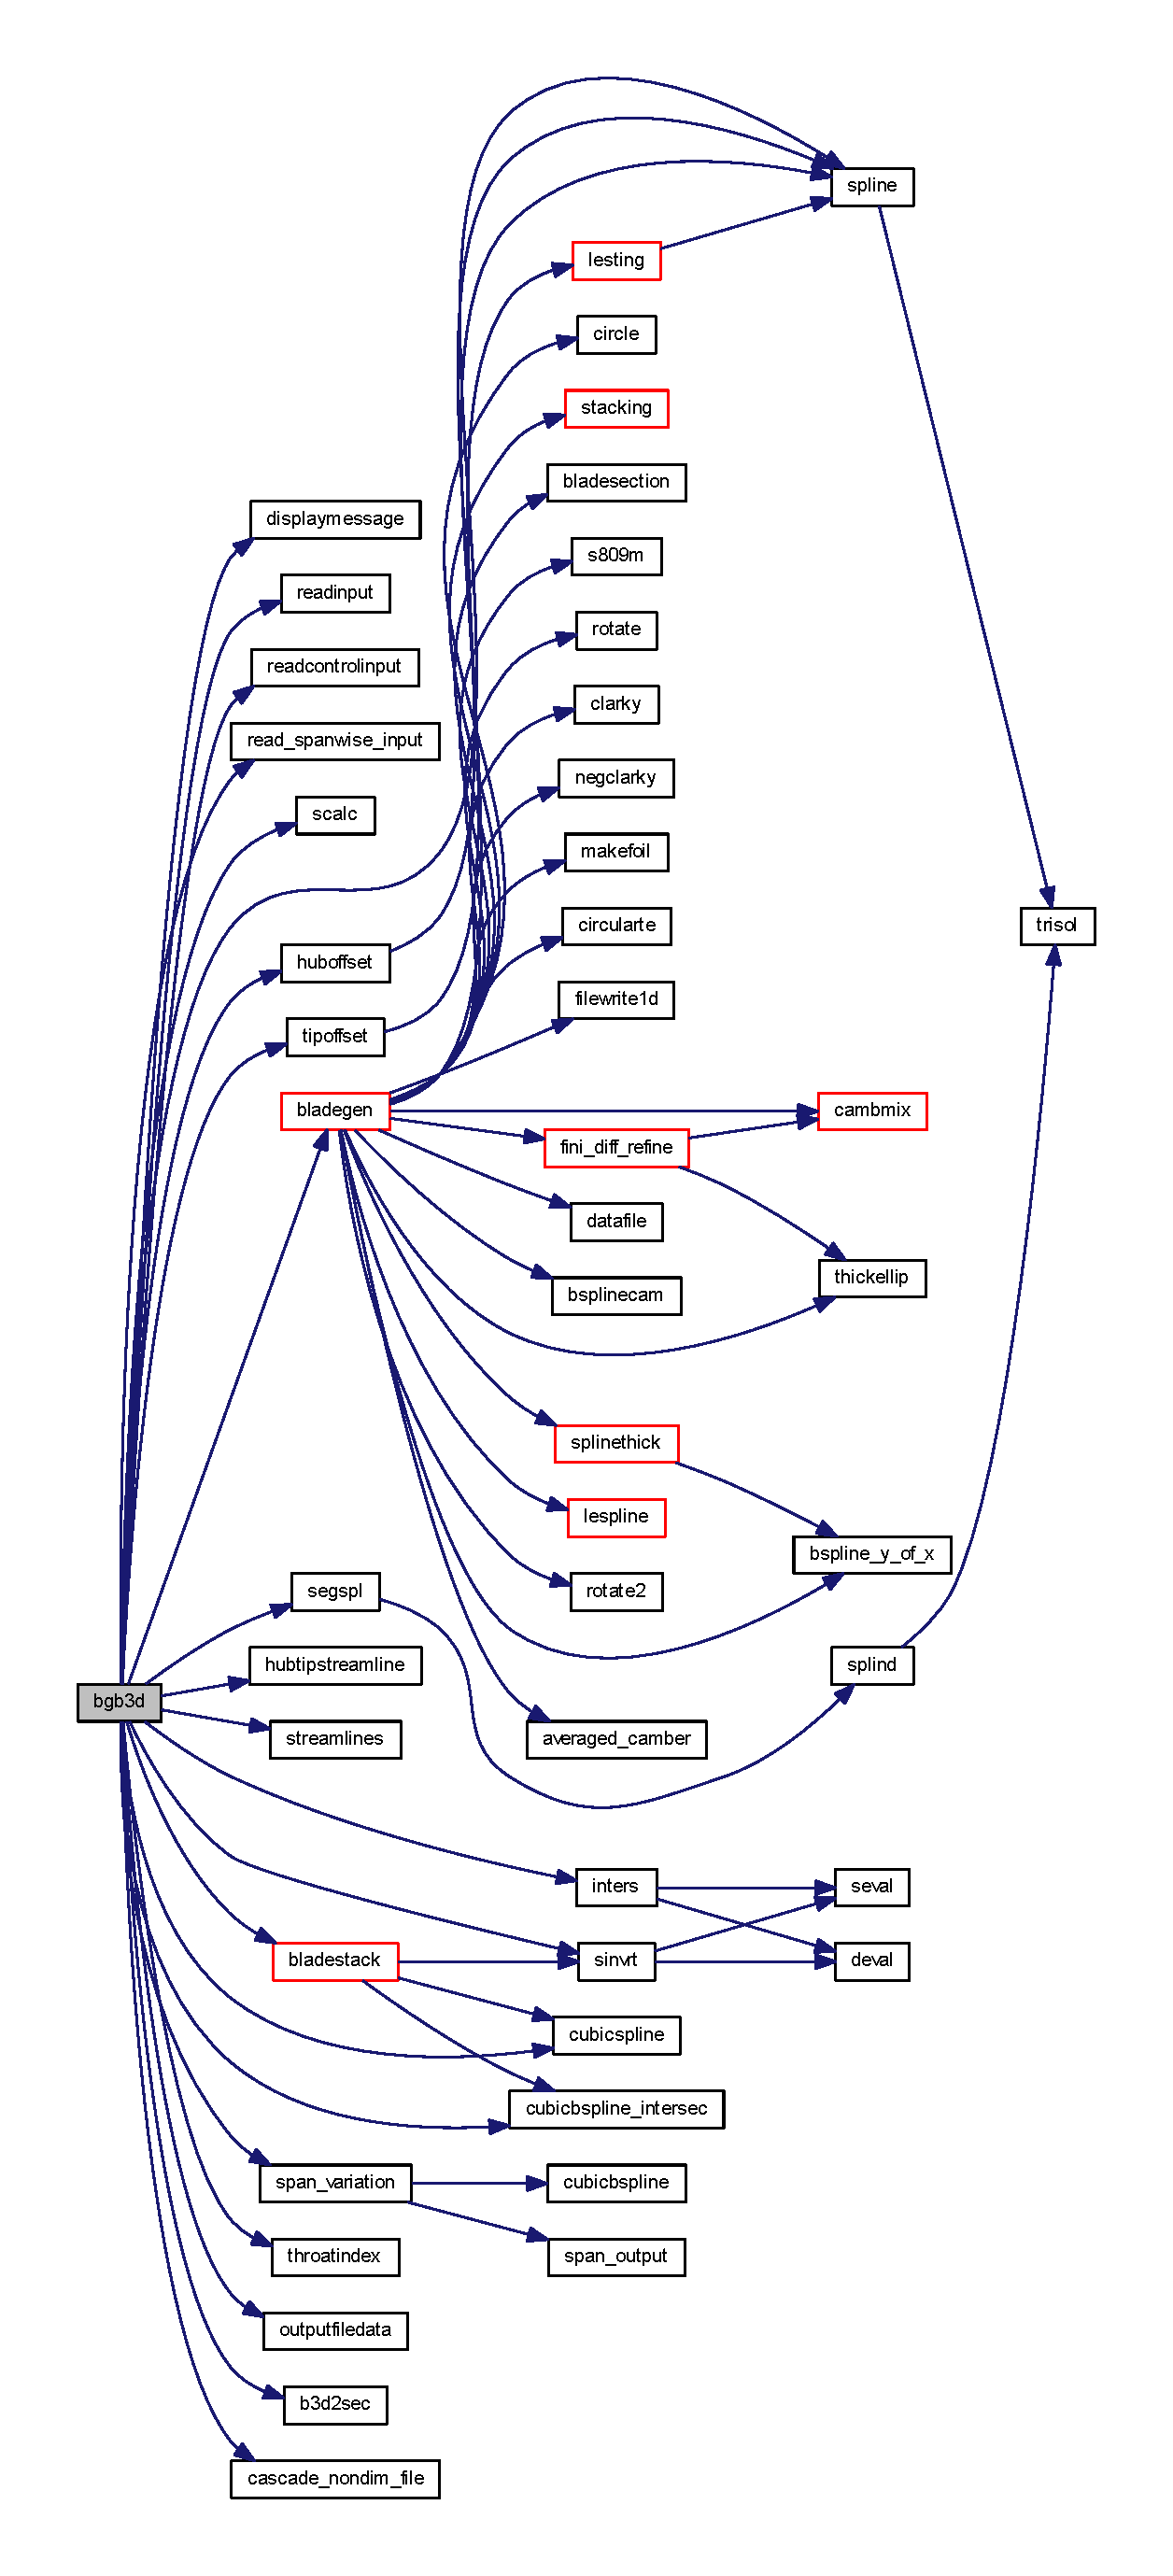
\includegraphics[height=550pt]{3dbgb_8f90_a0878a9e6406e3800984d6ffa80cbc560_cgraph}
\end{center}
\end{figure}



\hypertarget{airfoiltypes_8f90}{}\section{C\+:/\+Git3\+D\+B\+G\+B/source/airfoiltypes.f90 File Reference}
\label{airfoiltypes_8f90}\index{C\+:/\+Git3\+D\+B\+G\+B/source/airfoiltypes.\+f90@{C\+:/\+Git3\+D\+B\+G\+B/source/airfoiltypes.\+f90}}
\subsection*{Functions/\+Subroutines}
\begin{DoxyCompactItemize}
\item 
subroutine \hyperlink{airfoiltypes_8f90_a3856a45005e1ff6a6b5a66a8382dc8f3}{circle} (xb, yb, np)
\item 
subroutine \hyperlink{airfoiltypes_8f90_aa84a13e1320fe2e1eab9152e7fdb2df0}{s809m} (xb, yb, np)
\item 
subroutine \hyperlink{airfoiltypes_8f90_a6da6c16acb91da357dea201f88842610}{clarky} (xb, yb, np)
\item 
subroutine \hyperlink{airfoiltypes_8f90_a1bf682c66dd72805f48173e67201c849}{negclarky} (xb, yb, np)
\item 
subroutine \hyperlink{airfoiltypes_8f90_af5740105ff56b1b2168794605458ea38}{makefoil} (naca, xbot, ybot, xtop, ytop, np, x)
\item 
subroutine \hyperlink{airfoiltypes_8f90_a1a19cebda479d8a90783ab73bffa84f7}{datafile} (airfoil, xb, yb, np)
\item 
subroutine \hyperlink{airfoiltypes_8f90_abd280567076a4a22f4db89ad797773f5}{cambnaca} (u, cam, cam\+\_\+u, fmxcm, xmxcm)
\item 
subroutine \hyperlink{airfoiltypes_8f90_aeeba1d6343f34d391c0db6c40bf875bb}{thicknaca} (u, thk, fmxthk)
\item 
subroutine \hyperlink{airfoiltypes_8f90_adaace0fa9535fd4e8eb4a1e07819bdd2}{thickwen} (uin, thk, lethk, tethk, mxthk, umxthin, thkmultip)
\item 
subroutine \hyperlink{airfoiltypes_8f90_a4716e42043a5cad663238ac57e9662ef}{thickellip} (i, uin, thk, lethk, tethk, mxthk, umxthin, rr1, rr2, thkmultip                   ,u\+\_\+le, uin\+\_\+le, i\+\_\+le, oo, i\+\_\+te)
\item 
subroutine \hyperlink{airfoiltypes_8f90_a5f8930427d1cd12ba7d4120ec6a059e8}{cambcubic} (u, cam, cam\+\_\+u, s1, s2)
\item 
subroutine \hyperlink{airfoiltypes_8f90_ac00357f2293141bd7a6d9fbf23e9f03c}{cambmix} (u, cam, cam\+\_\+u, s1, s2, fl1, fl2)
\item 
subroutine \hyperlink{airfoiltypes_8f90_aa5fc53346a6f777f8f0e663027ec215f}{circularte} (xbot, ybot, xtop, ytop, np)
\end{DoxyCompactItemize}


\subsection{Function/\+Subroutine Documentation}
\hypertarget{airfoiltypes_8f90_a5f8930427d1cd12ba7d4120ec6a059e8}{}\index{airfoiltypes.\+f90@{airfoiltypes.\+f90}!cambcubic@{cambcubic}}
\index{cambcubic@{cambcubic}!airfoiltypes.\+f90@{airfoiltypes.\+f90}}
\subsubsection[{cambcubic(u, cam, cam\+\_\+u, s1, s2)}]{\setlength{\rightskip}{0pt plus 5cm}subroutine cambcubic (
\begin{DoxyParamCaption}
\item[{}]{u, }
\item[{}]{cam, }
\item[{}]{cam\+\_\+u, }
\item[{}]{s1, }
\item[{}]{s2}
\end{DoxyParamCaption}
)}\label{airfoiltypes_8f90_a5f8930427d1cd12ba7d4120ec6a059e8}
\hypertarget{airfoiltypes_8f90_ac00357f2293141bd7a6d9fbf23e9f03c}{}\index{airfoiltypes.\+f90@{airfoiltypes.\+f90}!cambmix@{cambmix}}
\index{cambmix@{cambmix}!airfoiltypes.\+f90@{airfoiltypes.\+f90}}
\subsubsection[{cambmix(u, cam, cam\+\_\+u, s1, s2, fl1, fl2)}]{\setlength{\rightskip}{0pt plus 5cm}subroutine cambmix (
\begin{DoxyParamCaption}
\item[{}]{u, }
\item[{}]{cam, }
\item[{}]{cam\+\_\+u, }
\item[{}]{s1, }
\item[{}]{s2, }
\item[{}]{fl1, }
\item[{}]{fl2}
\end{DoxyParamCaption}
)}\label{airfoiltypes_8f90_ac00357f2293141bd7a6d9fbf23e9f03c}


Here is the call graph for this function\+:
\nopagebreak
\begin{figure}[H]
\begin{center}
\leavevmode
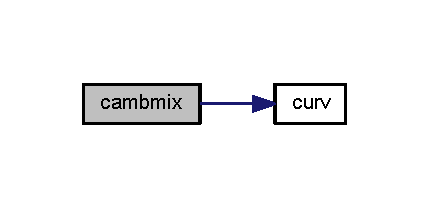
\includegraphics[width=206pt]{airfoiltypes_8f90_ac00357f2293141bd7a6d9fbf23e9f03c_cgraph}
\end{center}
\end{figure}




Here is the caller graph for this function\+:
\nopagebreak
\begin{figure}[H]
\begin{center}
\leavevmode
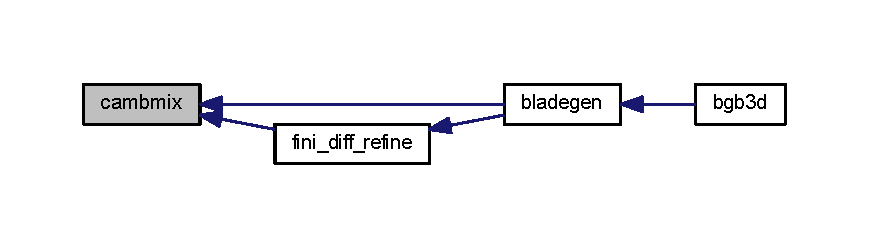
\includegraphics[width=350pt]{airfoiltypes_8f90_ac00357f2293141bd7a6d9fbf23e9f03c_icgraph}
\end{center}
\end{figure}


\hypertarget{airfoiltypes_8f90_abd280567076a4a22f4db89ad797773f5}{}\index{airfoiltypes.\+f90@{airfoiltypes.\+f90}!cambnaca@{cambnaca}}
\index{cambnaca@{cambnaca}!airfoiltypes.\+f90@{airfoiltypes.\+f90}}
\subsubsection[{cambnaca(u, cam, cam\+\_\+u, fmxcm, xmxcm)}]{\setlength{\rightskip}{0pt plus 5cm}subroutine cambnaca (
\begin{DoxyParamCaption}
\item[{}]{u, }
\item[{}]{cam, }
\item[{}]{cam\+\_\+u, }
\item[{}]{fmxcm, }
\item[{}]{xmxcm}
\end{DoxyParamCaption}
)}\label{airfoiltypes_8f90_abd280567076a4a22f4db89ad797773f5}
\hypertarget{airfoiltypes_8f90_a3856a45005e1ff6a6b5a66a8382dc8f3}{}\index{airfoiltypes.\+f90@{airfoiltypes.\+f90}!circle@{circle}}
\index{circle@{circle}!airfoiltypes.\+f90@{airfoiltypes.\+f90}}
\subsubsection[{circle(xb, yb, np)}]{\setlength{\rightskip}{0pt plus 5cm}subroutine circle (
\begin{DoxyParamCaption}
\item[{real, dimension(nx), intent(out)}]{xb, }
\item[{real, dimension(nx), intent(out)}]{yb, }
\item[{integer}]{np}
\end{DoxyParamCaption}
)}\label{airfoiltypes_8f90_a3856a45005e1ff6a6b5a66a8382dc8f3}


Here is the caller graph for this function\+:
\nopagebreak
\begin{figure}[H]
\begin{center}
\leavevmode
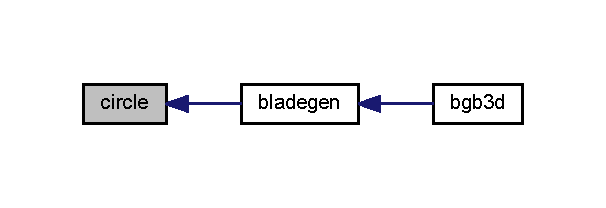
\includegraphics[width=291pt]{airfoiltypes_8f90_a3856a45005e1ff6a6b5a66a8382dc8f3_icgraph}
\end{center}
\end{figure}


\hypertarget{airfoiltypes_8f90_aa5fc53346a6f777f8f0e663027ec215f}{}\index{airfoiltypes.\+f90@{airfoiltypes.\+f90}!circularte@{circularte}}
\index{circularte@{circularte}!airfoiltypes.\+f90@{airfoiltypes.\+f90}}
\subsubsection[{circularte(xbot, ybot, xtop, ytop, np)}]{\setlength{\rightskip}{0pt plus 5cm}subroutine circularte (
\begin{DoxyParamCaption}
\item[{real$\ast$8, dimension(np), intent(inout)}]{xbot, }
\item[{real$\ast$8, dimension(np), intent(inout)}]{ybot, }
\item[{real$\ast$8, dimension(np), intent(inout)}]{xtop, }
\item[{real$\ast$8, dimension(np), intent(inout)}]{ytop, }
\item[{integer}]{np}
\end{DoxyParamCaption}
)}\label{airfoiltypes_8f90_aa5fc53346a6f777f8f0e663027ec215f}


Here is the caller graph for this function\+:
\nopagebreak
\begin{figure}[H]
\begin{center}
\leavevmode
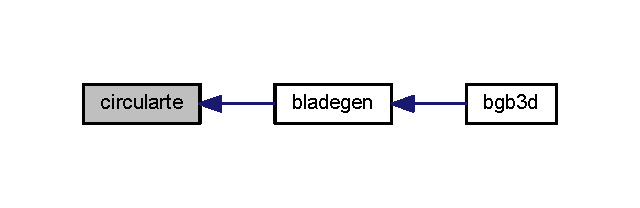
\includegraphics[width=307pt]{airfoiltypes_8f90_aa5fc53346a6f777f8f0e663027ec215f_icgraph}
\end{center}
\end{figure}


\hypertarget{airfoiltypes_8f90_a6da6c16acb91da357dea201f88842610}{}\index{airfoiltypes.\+f90@{airfoiltypes.\+f90}!clarky@{clarky}}
\index{clarky@{clarky}!airfoiltypes.\+f90@{airfoiltypes.\+f90}}
\subsubsection[{clarky(xb, yb, np)}]{\setlength{\rightskip}{0pt plus 5cm}subroutine clarky (
\begin{DoxyParamCaption}
\item[{real, dimension(nx), intent(out)}]{xb, }
\item[{real, dimension(nx), intent(out)}]{yb, }
\item[{integer}]{np}
\end{DoxyParamCaption}
)}\label{airfoiltypes_8f90_a6da6c16acb91da357dea201f88842610}


Here is the caller graph for this function\+:
\nopagebreak
\begin{figure}[H]
\begin{center}
\leavevmode
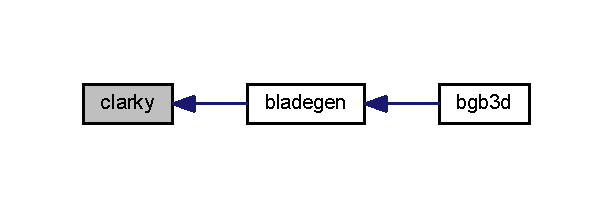
\includegraphics[width=294pt]{airfoiltypes_8f90_a6da6c16acb91da357dea201f88842610_icgraph}
\end{center}
\end{figure}


\hypertarget{airfoiltypes_8f90_a1a19cebda479d8a90783ab73bffa84f7}{}\index{airfoiltypes.\+f90@{airfoiltypes.\+f90}!datafile@{datafile}}
\index{datafile@{datafile}!airfoiltypes.\+f90@{airfoiltypes.\+f90}}
\subsubsection[{datafile(airfoil, xb, yb, np)}]{\setlength{\rightskip}{0pt plus 5cm}subroutine datafile (
\begin{DoxyParamCaption}
\item[{character $\ast$20}]{airfoil, }
\item[{real, dimension(nx), intent(out)}]{xb, }
\item[{real, dimension(nx), intent(out)}]{yb, }
\item[{integer}]{np}
\end{DoxyParamCaption}
)}\label{airfoiltypes_8f90_a1a19cebda479d8a90783ab73bffa84f7}


Here is the caller graph for this function\+:
\nopagebreak
\begin{figure}[H]
\begin{center}
\leavevmode
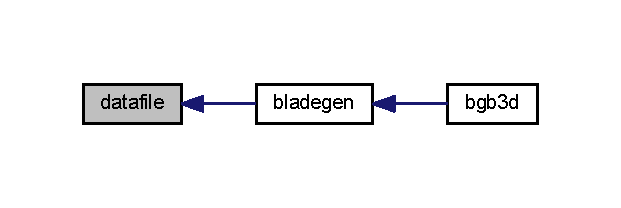
\includegraphics[width=298pt]{airfoiltypes_8f90_a1a19cebda479d8a90783ab73bffa84f7_icgraph}
\end{center}
\end{figure}


\hypertarget{airfoiltypes_8f90_af5740105ff56b1b2168794605458ea38}{}\index{airfoiltypes.\+f90@{airfoiltypes.\+f90}!makefoil@{makefoil}}
\index{makefoil@{makefoil}!airfoiltypes.\+f90@{airfoiltypes.\+f90}}
\subsubsection[{makefoil(naca, xbot, ybot, xtop, ytop, np, x)}]{\setlength{\rightskip}{0pt plus 5cm}subroutine makefoil (
\begin{DoxyParamCaption}
\item[{integer, intent(in)}]{naca, }
\item[{real, dimension(np), intent(out)}]{xbot, }
\item[{real, dimension(np), intent(out)}]{ybot, }
\item[{real, dimension(np), intent(out)}]{xtop, }
\item[{real, dimension(np), intent(out)}]{ytop, }
\item[{integer, intent(in)}]{np, }
\item[{real, dimension(np), intent(in)}]{x}
\end{DoxyParamCaption}
)}\label{airfoiltypes_8f90_af5740105ff56b1b2168794605458ea38}


Here is the caller graph for this function\+:
\nopagebreak
\begin{figure}[H]
\begin{center}
\leavevmode
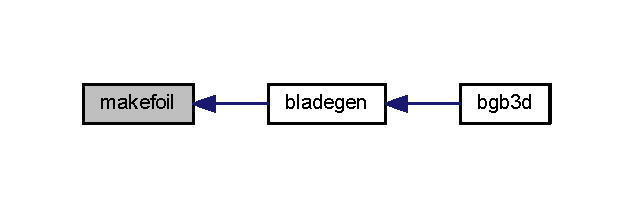
\includegraphics[width=304pt]{airfoiltypes_8f90_af5740105ff56b1b2168794605458ea38_icgraph}
\end{center}
\end{figure}


\hypertarget{airfoiltypes_8f90_a1bf682c66dd72805f48173e67201c849}{}\index{airfoiltypes.\+f90@{airfoiltypes.\+f90}!negclarky@{negclarky}}
\index{negclarky@{negclarky}!airfoiltypes.\+f90@{airfoiltypes.\+f90}}
\subsubsection[{negclarky(xb, yb, np)}]{\setlength{\rightskip}{0pt plus 5cm}subroutine negclarky (
\begin{DoxyParamCaption}
\item[{real, dimension(nx), intent(out)}]{xb, }
\item[{real, dimension(nx), intent(out)}]{yb, }
\item[{integer}]{np}
\end{DoxyParamCaption}
)}\label{airfoiltypes_8f90_a1bf682c66dd72805f48173e67201c849}


Here is the caller graph for this function\+:
\nopagebreak
\begin{figure}[H]
\begin{center}
\leavevmode
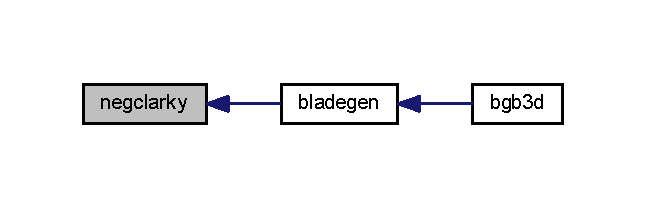
\includegraphics[width=310pt]{airfoiltypes_8f90_a1bf682c66dd72805f48173e67201c849_icgraph}
\end{center}
\end{figure}


\hypertarget{airfoiltypes_8f90_aa84a13e1320fe2e1eab9152e7fdb2df0}{}\index{airfoiltypes.\+f90@{airfoiltypes.\+f90}!s809m@{s809m}}
\index{s809m@{s809m}!airfoiltypes.\+f90@{airfoiltypes.\+f90}}
\subsubsection[{s809m(xb, yb, np)}]{\setlength{\rightskip}{0pt plus 5cm}subroutine s809m (
\begin{DoxyParamCaption}
\item[{real, dimension(nx), intent(out)}]{xb, }
\item[{real, dimension(nx), intent(out)}]{yb, }
\item[{integer}]{np}
\end{DoxyParamCaption}
)}\label{airfoiltypes_8f90_aa84a13e1320fe2e1eab9152e7fdb2df0}


Here is the caller graph for this function\+:
\nopagebreak
\begin{figure}[H]
\begin{center}
\leavevmode
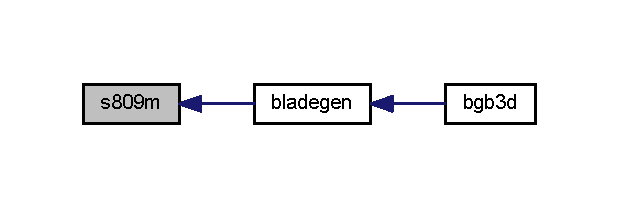
\includegraphics[width=297pt]{airfoiltypes_8f90_aa84a13e1320fe2e1eab9152e7fdb2df0_icgraph}
\end{center}
\end{figure}


\hypertarget{airfoiltypes_8f90_a4716e42043a5cad663238ac57e9662ef}{}\index{airfoiltypes.\+f90@{airfoiltypes.\+f90}!thickellip@{thickellip}}
\index{thickellip@{thickellip}!airfoiltypes.\+f90@{airfoiltypes.\+f90}}
\subsubsection[{thickellip(i, uin, thk, lethk, tethk, mxthk, umxthin, rr1, rr2, thkmultip                   ,u\+\_\+le, uin\+\_\+le, i\+\_\+le, oo, i\+\_\+te)}]{\setlength{\rightskip}{0pt plus 5cm}subroutine thickellip (
\begin{DoxyParamCaption}
\item[{integer}]{i, }
\item[{}]{uin, }
\item[{}]{thk, }
\item[{real}]{lethk, }
\item[{real}]{tethk, }
\item[{real}]{mxthk, }
\item[{}]{umxthin, }
\item[{}]{rr1, }
\item[{}]{rr2, }
\item[{real}]{thkmultip, }
\item[{real}]{u\+\_\+le, }
\item[{real}]{uin\+\_\+le, }
\item[{integer}]{i\+\_\+le, }
\item[{integer}]{oo, }
\item[{integer}]{i\+\_\+te}
\end{DoxyParamCaption}
)}\label{airfoiltypes_8f90_a4716e42043a5cad663238ac57e9662ef}


Here is the caller graph for this function\+:
\nopagebreak
\begin{figure}[H]
\begin{center}
\leavevmode
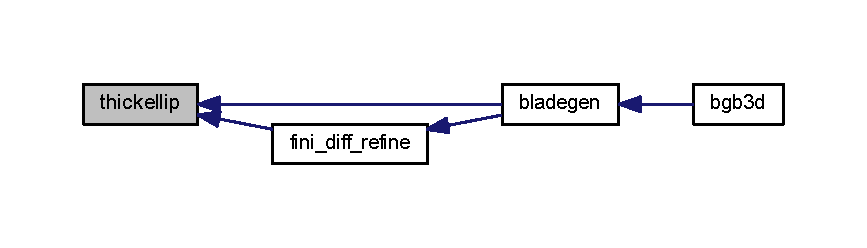
\includegraphics[width=350pt]{airfoiltypes_8f90_a4716e42043a5cad663238ac57e9662ef_icgraph}
\end{center}
\end{figure}


\hypertarget{airfoiltypes_8f90_aeeba1d6343f34d391c0db6c40bf875bb}{}\index{airfoiltypes.\+f90@{airfoiltypes.\+f90}!thicknaca@{thicknaca}}
\index{thicknaca@{thicknaca}!airfoiltypes.\+f90@{airfoiltypes.\+f90}}
\subsubsection[{thicknaca(u, thk, fmxthk)}]{\setlength{\rightskip}{0pt plus 5cm}subroutine thicknaca (
\begin{DoxyParamCaption}
\item[{}]{u, }
\item[{}]{thk, }
\item[{}]{fmxthk}
\end{DoxyParamCaption}
)}\label{airfoiltypes_8f90_aeeba1d6343f34d391c0db6c40bf875bb}
\hypertarget{airfoiltypes_8f90_adaace0fa9535fd4e8eb4a1e07819bdd2}{}\index{airfoiltypes.\+f90@{airfoiltypes.\+f90}!thickwen@{thickwen}}
\index{thickwen@{thickwen}!airfoiltypes.\+f90@{airfoiltypes.\+f90}}
\subsubsection[{thickwen(uin, thk, lethk, tethk, mxthk, umxthin, thkmultip)}]{\setlength{\rightskip}{0pt plus 5cm}subroutine thickwen (
\begin{DoxyParamCaption}
\item[{}]{uin, }
\item[{}]{thk, }
\item[{real}]{lethk, }
\item[{real}]{tethk, }
\item[{real}]{mxthk, }
\item[{}]{umxthin, }
\item[{real}]{thkmultip}
\end{DoxyParamCaption}
)}\label{airfoiltypes_8f90_adaace0fa9535fd4e8eb4a1e07819bdd2}

\hypertarget{b3d2sec_8f90}{}\section{C\+:/\+Git3\+D\+B\+G\+B/source/b3d2sec.f90 File Reference}
\label{b3d2sec_8f90}\index{C\+:/\+Git3\+D\+B\+G\+B/source/b3d2sec.\+f90@{C\+:/\+Git3\+D\+B\+G\+B/source/b3d2sec.\+f90}}
\subsection*{Functions/\+Subroutines}
\begin{DoxyCompactItemize}
\item 
subroutine \hyperlink{b3d2sec_8f90_ac5919be8e11c167fec3b16c05090ae91}{b3d2sec} (scf, fext, ibrowc, nbls, casename)
\end{DoxyCompactItemize}


\subsection{Function/\+Subroutine Documentation}
\hypertarget{b3d2sec_8f90_ac5919be8e11c167fec3b16c05090ae91}{}\index{b3d2sec.\+f90@{b3d2sec.\+f90}!b3d2sec@{b3d2sec}}
\index{b3d2sec@{b3d2sec}!b3d2sec.\+f90@{b3d2sec.\+f90}}
\subsubsection[{b3d2sec(scf, fext, ibrowc, nbls, casename)}]{\setlength{\rightskip}{0pt plus 5cm}subroutine b3d2sec (
\begin{DoxyParamCaption}
\item[{real$\ast$8}]{scf, }
\item[{character$\ast$32}]{fext, }
\item[{character$\ast$10}]{ibrowc, }
\item[{integer}]{nbls, }
\item[{character$\ast$32}]{casename}
\end{DoxyParamCaption}
)}\label{b3d2sec_8f90_ac5919be8e11c167fec3b16c05090ae91}


Here is the caller graph for this function\+:
\nopagebreak
\begin{figure}[H]
\begin{center}
\leavevmode
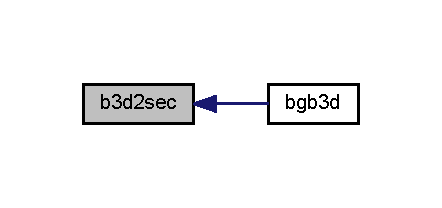
\includegraphics[width=212pt]{b3d2sec_8f90_ac5919be8e11c167fec3b16c05090ae91_icgraph}
\end{center}
\end{figure}



\hypertarget{bladegen_8f90}{}\section{C\+:/\+Git3\+D\+B\+G\+B/source/bladegen.f90 File Reference}
\label{bladegen_8f90}\index{C\+:/\+Git3\+D\+B\+G\+B/source/bladegen.\+f90@{C\+:/\+Git3\+D\+B\+G\+B/source/bladegen.\+f90}}
\subsection*{Functions/\+Subroutines}
\begin{DoxyCompactItemize}
\item 
subroutine \hyperlink{bladegen_8f90_abe1d53034e73a0fd4caf61124de7e6eb}{bladegen} (nspn, thkc, mr1, sinl, sext, chrdx, js, fext, xcen, ycen, airfoil,                                                                           stagger, stack, chord\+\_\+switch, stk\+\_\+u, stk\+\_\+v, xb\+\_\+stk, yb\+\_\+stk, stack\+\_\+switch,                                                                           nsl, nbls, curv\+\_\+camber, thick, L\+E, np, ncp\+\_\+curv, ncp\+\_\+thk, curv\+\_\+cp, thk\+\_\+cp,                                                                           lethk\+\_\+all, tethk\+\_\+all, s\+\_\+all, ee\+\_\+all, thick\+\_\+distr, umxthk\+\_\+all,                                                       C\+\_\+le\+\_\+x\+\_\+top\+\_\+all, C\+\_\+le\+\_\+x\+\_\+bot\+\_\+all, C\+\_\+le\+\_\+y\+\_\+top\+\_\+all, C\+\_\+le\+\_\+y\+\_\+bot\+\_\+all,                                                       L\+E\+\_\+vertex\+\_\+ang\+\_\+all, L\+E\+\_\+vertex\+\_\+dis\+\_\+all, sting\+\_\+l\+\_\+all, sting\+\_\+h\+\_\+all, L\+Edegree, no\+\_\+\+L\+E\+\_\+segments,                                                       sec\+\_\+radius, bladedata, amount\+\_\+data, scf, intersec\+\_\+coord, throat\+\_\+index,                                                                           n\+\_\+normal\+\_\+distance, casename, develop, isdev, mble, mbte, msle, mste, i\+\_\+slope, jcellblade\+\_\+all,                                                                           etawidth\+\_\+all, B\+Ggrid\+\_\+all, thk\+\_\+tm\+\_\+c\+\_\+spl, isxygrid)
\end{DoxyCompactItemize}


\subsection{Function/\+Subroutine Documentation}
\hypertarget{bladegen_8f90_abe1d53034e73a0fd4caf61124de7e6eb}{}\index{bladegen.\+f90@{bladegen.\+f90}!bladegen@{bladegen}}
\index{bladegen@{bladegen}!bladegen.\+f90@{bladegen.\+f90}}
\subsubsection[{bladegen(nspn, thkc, mr1, sinl, sext, chrdx, js, fext, xcen, ycen, airfoil,                                                                           stagger, stack, chord\+\_\+switch, stk\+\_\+u, stk\+\_\+v, xb\+\_\+stk, yb\+\_\+stk, stack\+\_\+switch,                                                                           nsl, nbls, curv\+\_\+camber, thick, L\+E, np, ncp\+\_\+curv, ncp\+\_\+thk, curv\+\_\+cp, thk\+\_\+cp,                                                                           lethk\+\_\+all, tethk\+\_\+all, s\+\_\+all, ee\+\_\+all, thick\+\_\+distr, umxthk\+\_\+all,                                                       C\+\_\+le\+\_\+x\+\_\+top\+\_\+all, C\+\_\+le\+\_\+x\+\_\+bot\+\_\+all, C\+\_\+le\+\_\+y\+\_\+top\+\_\+all, C\+\_\+le\+\_\+y\+\_\+bot\+\_\+all,                                                       L\+E\+\_\+vertex\+\_\+ang\+\_\+all, L\+E\+\_\+vertex\+\_\+dis\+\_\+all, sting\+\_\+l\+\_\+all, sting\+\_\+h\+\_\+all, L\+Edegree, no\+\_\+\+L\+E\+\_\+segments,                                                       sec\+\_\+radius, bladedata, amount\+\_\+data, scf, intersec\+\_\+coord, throat\+\_\+index,                                                                           n\+\_\+normal\+\_\+distance, casename, develop, isdev, mble, mbte, msle, mste, i\+\_\+slope, jcellblade\+\_\+all,                                                                           etawidth\+\_\+all, B\+Ggrid\+\_\+all, thk\+\_\+tm\+\_\+c\+\_\+spl, isxygrid)}]{\setlength{\rightskip}{0pt plus 5cm}subroutine bladegen (
\begin{DoxyParamCaption}
\item[{integer}]{nspn, }
\item[{real}]{thkc, }
\item[{real}]{mr1, }
\item[{real}]{sinl, }
\item[{real}]{sext, }
\item[{real}]{chrdx, }
\item[{integer}]{js, }
\item[{character$\ast$32}]{fext, }
\item[{real}]{xcen, }
\item[{real}]{ycen, }
\item[{character$\ast$20}]{airfoil, }
\item[{real}]{stagger, }
\item[{integer}]{stack, }
\item[{integer}]{chord\+\_\+switch, }
\item[{real, dimension(1)}]{stk\+\_\+u, }
\item[{real, dimension(1)}]{stk\+\_\+v, }
\item[{real}]{xb\+\_\+stk, }
\item[{real}]{yb\+\_\+stk, }
\item[{integer}]{stack\+\_\+switch, }
\item[{integer}]{nsl, }
\item[{integer}]{nbls, }
\item[{integer}]{curv\+\_\+camber, }
\item[{integer}]{thick, }
\item[{integer}]{L\+E, }
\item[{integer}]{np, }
\item[{integer, dimension(nsl)}]{ncp\+\_\+curv, }
\item[{integer, dimension(nsl)}]{ncp\+\_\+thk, }
\item[{real, dimension(20,2$\ast$nsl)}]{curv\+\_\+cp, }
\item[{real, dimension(20,2$\ast$nsl)}]{thk\+\_\+cp, }
\item[{real, dimension(nsl)}]{lethk\+\_\+all, }
\item[{real, dimension(nsl)}]{tethk\+\_\+all, }
\item[{real, dimension(nsl)}]{s\+\_\+all, }
\item[{real, dimension(nsl)}]{ee\+\_\+all, }
\item[{integer}]{thick\+\_\+distr, }
\item[{real, dimension(nsl)}]{umxthk\+\_\+all, }
\item[{real, dimension(nsl)}]{C\+\_\+le\+\_\+x\+\_\+top\+\_\+all, }
\item[{real, dimension(nsl)}]{C\+\_\+le\+\_\+x\+\_\+bot\+\_\+all, }
\item[{real, dimension(nsl)}]{C\+\_\+le\+\_\+y\+\_\+top\+\_\+all, }
\item[{real, dimension(nsl)}]{C\+\_\+le\+\_\+y\+\_\+bot\+\_\+all, }
\item[{real, dimension(nsl)}]{L\+E\+\_\+vertex\+\_\+ang\+\_\+all, }
\item[{real, dimension(nsl)}]{L\+E\+\_\+vertex\+\_\+dis\+\_\+all, }
\item[{real, dimension(nsl)}]{sting\+\_\+l\+\_\+all, }
\item[{real, dimension(nsl,2)}]{sting\+\_\+h\+\_\+all, }
\item[{integer}]{L\+Edegree, }
\item[{integer}]{no\+\_\+\+L\+E\+\_\+segments, }
\item[{real, dimension(nsl,2)}]{sec\+\_\+radius, }
\item[{real$\ast$4, dimension(amount\+\_\+data,nsl)}]{bladedata, }
\item[{integer}]{amount\+\_\+data, }
\item[{real}]{scf, }
\item[{real, dimension(12,nsl)}]{intersec\+\_\+coord, }
\item[{integer, dimension(nspn)}]{throat\+\_\+index, }
\item[{integer}]{n\+\_\+normal\+\_\+distance, }
\item[{character$\ast$32}]{casename, }
\item[{character$\ast$32}]{develop, }
\item[{logical}]{isdev, }
\item[{real}]{mble, }
\item[{real}]{mbte, }
\item[{real}]{msle, }
\item[{real}]{mste, }
\item[{integer}]{i\+\_\+slope, }
\item[{real, dimension(nspn)}]{jcellblade\+\_\+all, }
\item[{real, dimension(nspn)}]{etawidth\+\_\+all, }
\item[{integer, dimension(nspn)}]{B\+Ggrid\+\_\+all, }
\item[{real, dimension(nsl)}]{thk\+\_\+tm\+\_\+c\+\_\+spl, }
\item[{logical}]{isxygrid}
\end{DoxyParamCaption}
)}\label{bladegen_8f90_abe1d53034e73a0fd4caf61124de7e6eb}


Here is the call graph for this function\+:
\nopagebreak
\begin{figure}[H]
\begin{center}
\leavevmode
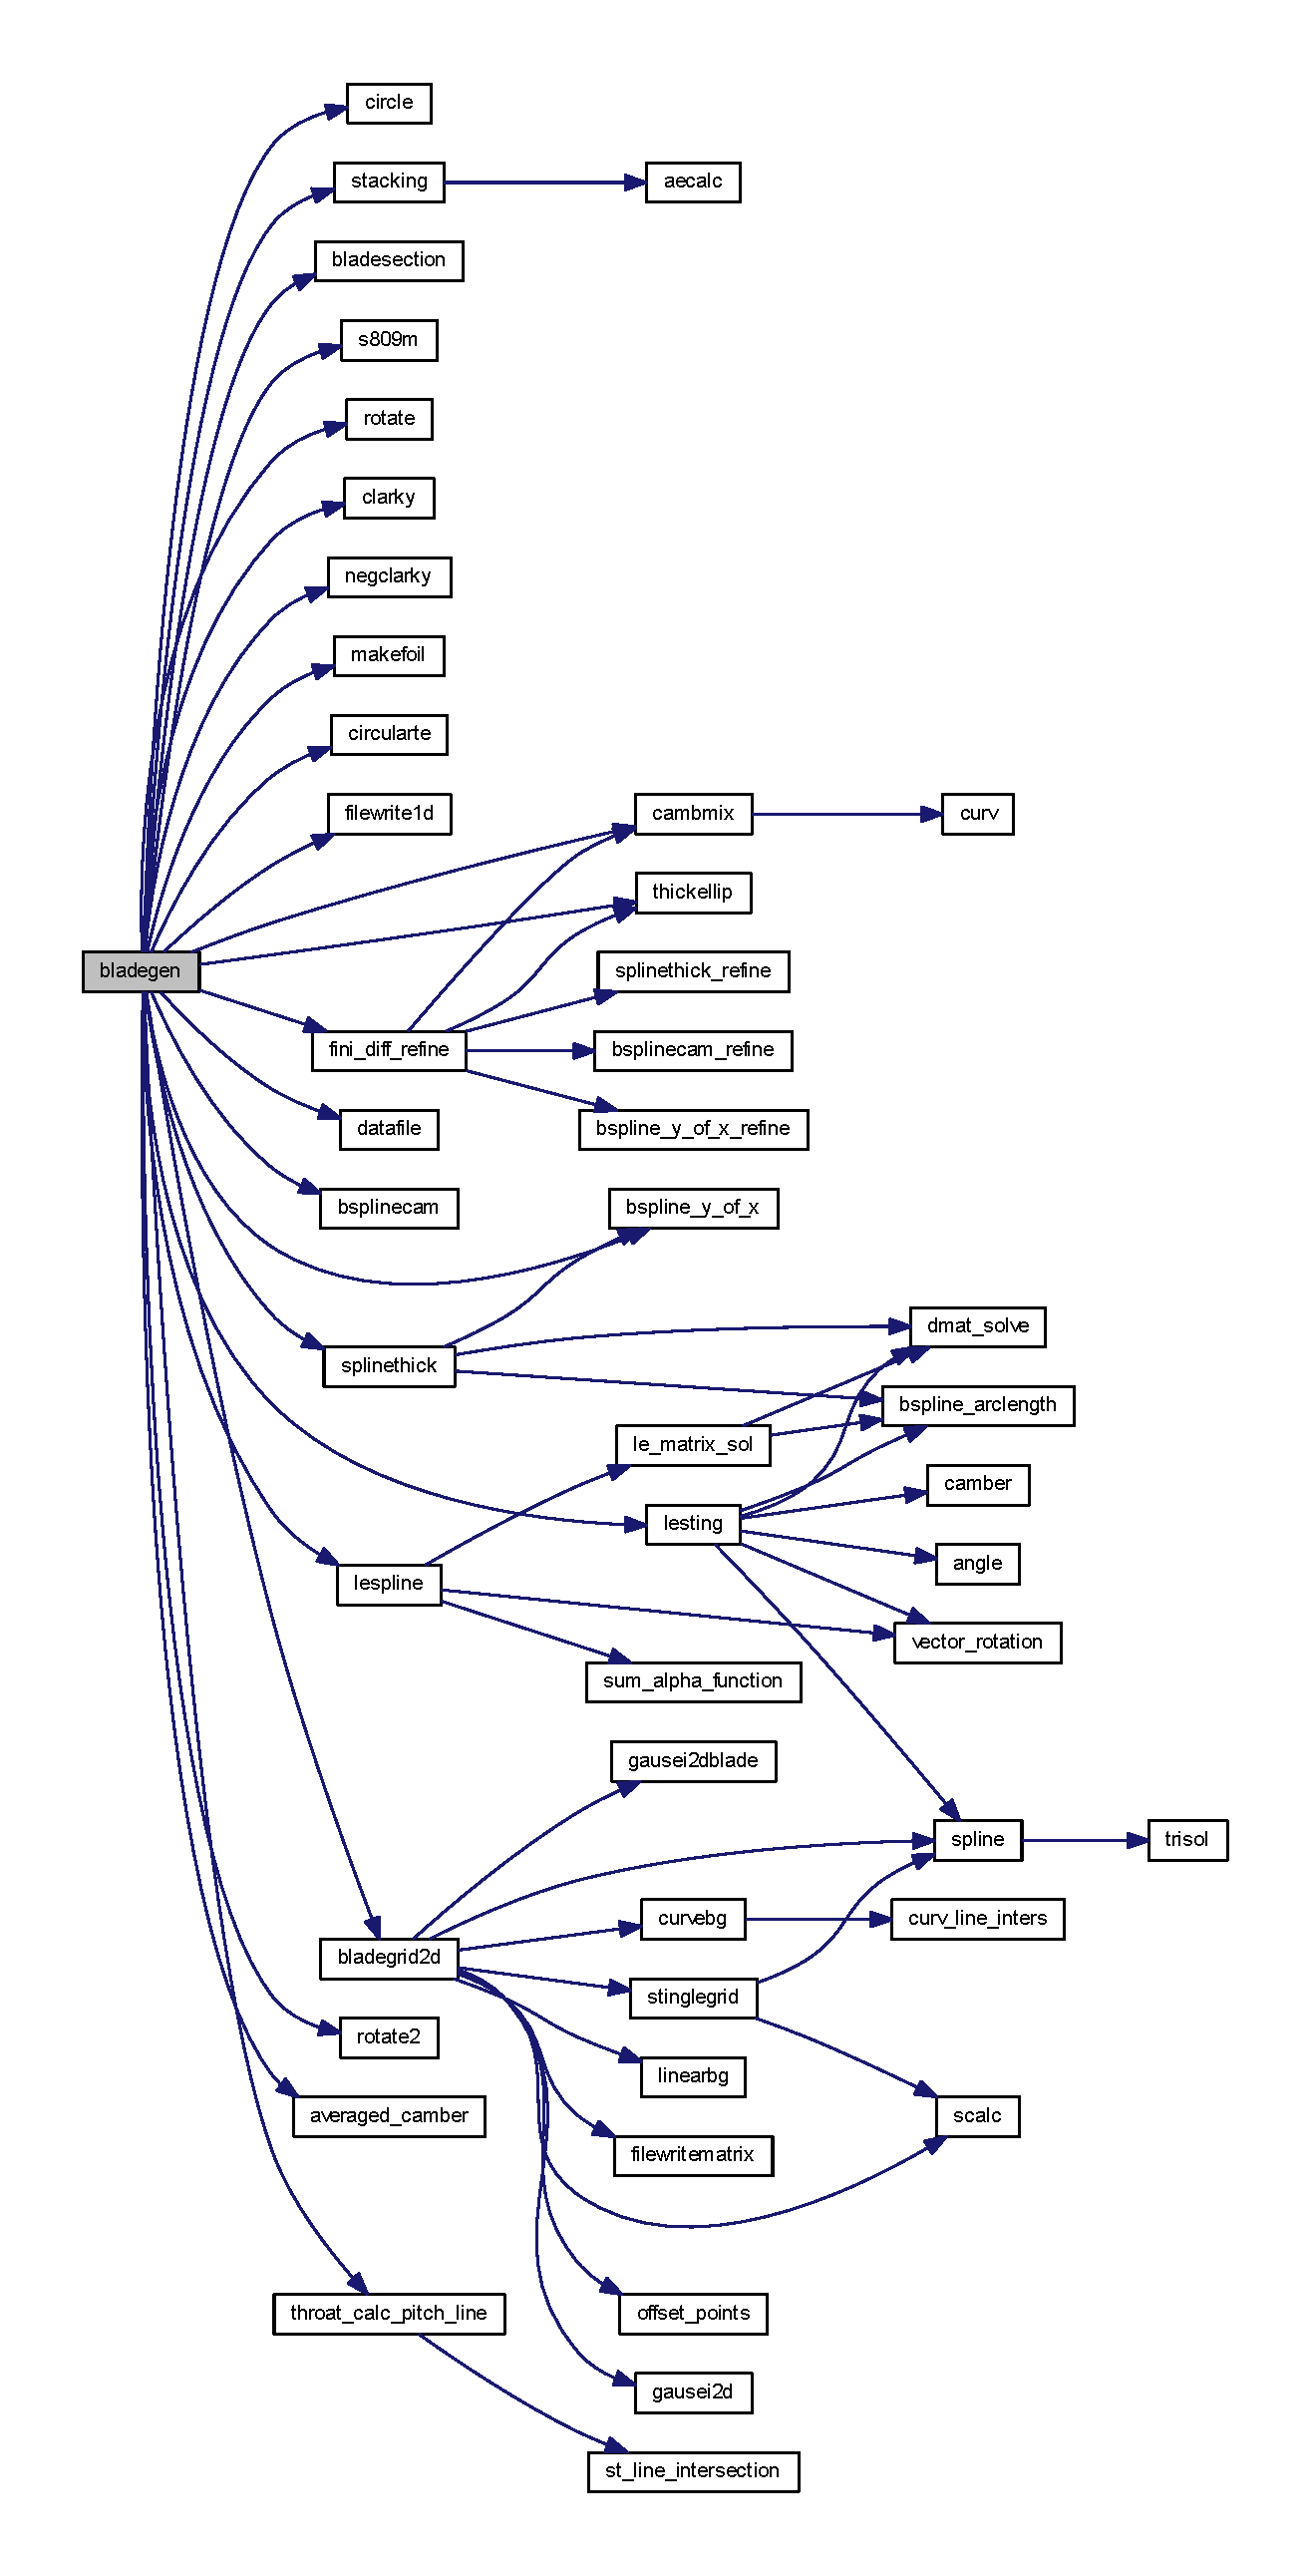
\includegraphics[height=550pt]{bladegen_8f90_abe1d53034e73a0fd4caf61124de7e6eb_cgraph}
\end{center}
\end{figure}




Here is the caller graph for this function\+:
\nopagebreak
\begin{figure}[H]
\begin{center}
\leavevmode
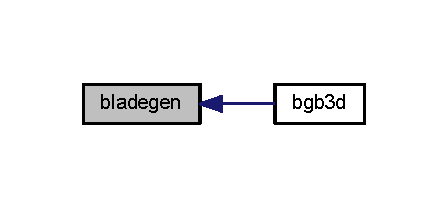
\includegraphics[width=215pt]{bladegen_8f90_abe1d53034e73a0fd4caf61124de7e6eb_icgraph}
\end{center}
\end{figure}



\hypertarget{bladegrid2_d_8f90}{}\section{C\+:/\+Git3\+D\+B\+G\+B/source/bladegrid2\+D.f90 File Reference}
\label{bladegrid2_d_8f90}\index{C\+:/\+Git3\+D\+B\+G\+B/source/bladegrid2\+D.\+f90@{C\+:/\+Git3\+D\+B\+G\+B/source/bladegrid2\+D.\+f90}}
\subsection*{Functions/\+Subroutines}
\begin{DoxyCompactItemize}
\item 
subroutine \hyperlink{bladegrid2_d_8f90_a942de4324f4b58cfa677173c90eae2b6}{bladegrid2d} (xb, yb, np, nbls, chrd, thkc, fext, L\+E, le\+\_\+pos, thick\+\_\+distr,                                                                                       casename, msle, mste, mble, mbte, js, nspn, np\+\_\+side,                                                                                       curv\+\_\+camber, stingl, jcellblade, etawidth, B\+Ggrid, develop, isdev)
\end{DoxyCompactItemize}


\subsection{Function/\+Subroutine Documentation}
\hypertarget{bladegrid2_d_8f90_a942de4324f4b58cfa677173c90eae2b6}{}\index{bladegrid2\+D.\+f90@{bladegrid2\+D.\+f90}!bladegrid2d@{bladegrid2d}}
\index{bladegrid2d@{bladegrid2d}!bladegrid2\+D.\+f90@{bladegrid2\+D.\+f90}}
\subsubsection[{bladegrid2d(xb, yb, np, nbls, chrd, thkc, fext, L\+E, le\+\_\+pos, thick\+\_\+distr,                                                                                       casename, msle, mste, mble, mbte, js, nspn, np\+\_\+side,                                                                                       curv\+\_\+camber, stingl, jcellblade, etawidth, B\+Ggrid, develop, isdev)}]{\setlength{\rightskip}{0pt plus 5cm}subroutine bladegrid2d (
\begin{DoxyParamCaption}
\item[{real$\ast$8, dimension(np)}]{xb, }
\item[{real$\ast$8, dimension(np)}]{yb, }
\item[{integer}]{np, }
\item[{integer}]{nbls, }
\item[{real$\ast$8}]{chrd, }
\item[{real$\ast$8}]{thkc, }
\item[{character$\ast$32}]{fext, }
\item[{integer}]{L\+E, }
\item[{integer}]{le\+\_\+pos, }
\item[{real$\ast$8}]{thick\+\_\+distr, }
\item[{character$\ast$32}]{casename, }
\item[{real$\ast$8}]{msle, }
\item[{real$\ast$8}]{mste, }
\item[{real$\ast$8}]{mble, }
\item[{real$\ast$8}]{mbte, }
\item[{integer}]{js, }
\item[{integer}]{nspn, }
\item[{integer}]{np\+\_\+side, }
\item[{integer}]{curv\+\_\+camber, }
\item[{real$\ast$8}]{stingl, }
\item[{real$\ast$8}]{jcellblade, }
\item[{real$\ast$8}]{etawidth, }
\item[{integer}]{B\+Ggrid, }
\item[{character$\ast$32}]{develop, }
\item[{logical}]{isdev}
\end{DoxyParamCaption}
)}\label{bladegrid2_d_8f90_a942de4324f4b58cfa677173c90eae2b6}


Here is the call graph for this function\+:
\nopagebreak
\begin{figure}[H]
\begin{center}
\leavevmode
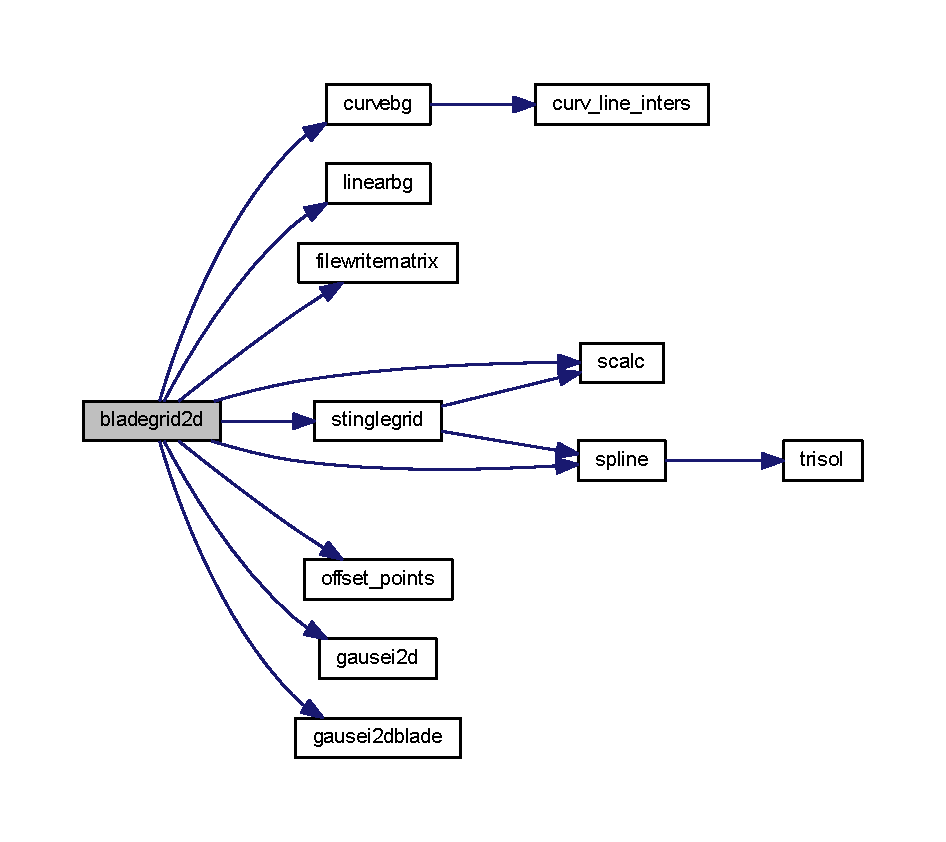
\includegraphics[width=350pt]{bladegrid2_d_8f90_a942de4324f4b58cfa677173c90eae2b6_cgraph}
\end{center}
\end{figure}




Here is the caller graph for this function\+:
\nopagebreak
\begin{figure}[H]
\begin{center}
\leavevmode
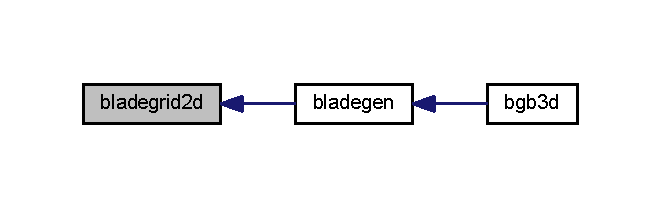
\includegraphics[width=317pt]{bladegrid2_d_8f90_a942de4324f4b58cfa677173c90eae2b6_icgraph}
\end{center}
\end{figure}



\hypertarget{bladestack_8f90}{}\section{C\+:/\+Git3\+D\+B\+G\+B/source/bladestack.f90 File Reference}
\label{bladestack_8f90}\index{C\+:/\+Git3\+D\+B\+G\+B/source/bladestack.\+f90@{C\+:/\+Git3\+D\+B\+G\+B/source/bladestack.\+f90}}
\subsection*{Functions/\+Subroutines}
\begin{DoxyCompactItemize}
\item 
subroutine \hyperlink{bladestack_8f90_a5dab74068855acf2e6917b70290ac7ec}{bladestack} (nspn, X\+\_\+le, X\+\_\+te, R\+\_\+le, R\+\_\+te, nsec, scf, xcg, ycg, msle, stk\+\_\+u, stk\+\_\+v, xb\+\_\+stack, yb\+\_\+stack, np, iile, stack, cpdeltam, spanmp, xcpdelm, cpdeltheta, spantheta, xcpdeltheta, cpinbeta, spaninbeta, xcpinbeta, cpoutbeta, spanoutbeta, xcpoutbeta, hub, tip, xm, rm, xms, rms, mp, nsp, bladedata, amount\+\_\+data, intersec\+\_\+coord, throat\+\_\+3\+D, mouth\+\_\+3\+D, exit\+\_\+3\+D, casename, nbls, L\+E, axchrd, mble,                                                                           mbte, units, stagger, chrdsweep, chrdlean, axial\+\_\+\+L\+E, radial\+\_\+\+L\+E)
\end{DoxyCompactItemize}


\subsection{Function/\+Subroutine Documentation}
\hypertarget{bladestack_8f90_a5dab74068855acf2e6917b70290ac7ec}{}\index{bladestack.\+f90@{bladestack.\+f90}!bladestack@{bladestack}}
\index{bladestack@{bladestack}!bladestack.\+f90@{bladestack.\+f90}}
\subsubsection[{bladestack(nspn, X\+\_\+le, X\+\_\+te, R\+\_\+le, R\+\_\+te, nsec, scf, xcg, ycg, msle, stk\+\_\+u, stk\+\_\+v, xb\+\_\+stack, yb\+\_\+stack, np, iile, stack, cpdeltam, spanmp, xcpdelm, cpdeltheta, spantheta, xcpdeltheta, cpinbeta, spaninbeta, xcpinbeta, cpoutbeta, spanoutbeta, xcpoutbeta, hub, tip, xm, rm, xms, rms, mp, nsp, bladedata, amount\+\_\+data, intersec\+\_\+coord, throat\+\_\+3\+D, mouth\+\_\+3\+D, exit\+\_\+3\+D, casename, nbls, L\+E, axchrd, mble,                                                                           mbte, units, stagger, chrdsweep, chrdlean, axial\+\_\+\+L\+E, radial\+\_\+\+L\+E)}]{\setlength{\rightskip}{0pt plus 5cm}subroutine bladestack (
\begin{DoxyParamCaption}
\item[{integer}]{nspn, }
\item[{real, dimension(nspan)}]{X\+\_\+le, }
\item[{real, dimension(nspan)}]{X\+\_\+te, }
\item[{real, dimension(nspan)}]{R\+\_\+le, }
\item[{real, dimension(nspan)}]{R\+\_\+te, }
\item[{integer}]{nsec, }
\item[{real}]{scf, }
\item[{real, dimension(nspan)}]{xcg, }
\item[{real, dimension(nspan)}]{ycg, }
\item[{real, dimension(nspan)}]{msle, }
\item[{integer}]{stk\+\_\+u, }
\item[{integer}]{stk\+\_\+v, }
\item[{real, dimension(nspan)}]{xb\+\_\+stack, }
\item[{real, dimension(nspan)}]{yb\+\_\+stack, }
\item[{integer}]{np, }
\item[{integer}]{iile, }
\item[{integer}]{stack, }
\item[{integer}]{cpdeltam, }
\item[{real$\ast$8, dimension(100)}]{spanmp, }
\item[{real$\ast$8, dimension(100)}]{xcpdelm, }
\item[{integer}]{cpdeltheta, }
\item[{real$\ast$8, dimension(100)}]{spantheta, }
\item[{real$\ast$8, dimension(100)}]{xcpdeltheta, }
\item[{integer}]{cpinbeta, }
\item[{real$\ast$8, dimension(100)}]{spaninbeta, }
\item[{real$\ast$8, dimension(100)}]{xcpinbeta, }
\item[{integer}]{cpoutbeta, }
\item[{real$\ast$8, dimension(100)}]{spanoutbeta, }
\item[{real$\ast$8, dimension(100)}]{xcpoutbeta, }
\item[{real}]{hub, }
\item[{real}]{tip, }
\item[{real, dimension(nx,nax)}]{xm, }
\item[{real, dimension(nx,nax)}]{rm, }
\item[{real, dimension(nx,nax)}]{xms, }
\item[{real, dimension(nx,nax)}]{rms, }
\item[{real, dimension(nx,nax)}]{mp, }
\item[{integer, dimension(nspan)}]{nsp, }
\item[{real$\ast$4, dimension(amount\+\_\+data,nspn)}]{bladedata, }
\item[{integer}]{amount\+\_\+data, }
\item[{real, dimension(12,nspn)}]{intersec\+\_\+coord, }
\item[{real, dimension(nspn)}]{throat\+\_\+3\+D, }
\item[{real, dimension(nspn)}]{mouth\+\_\+3\+D, }
\item[{real, dimension(nspn)}]{exit\+\_\+3\+D, }
\item[{character$\ast$32}]{casename, }
\item[{integer}]{nbls, }
\item[{integer}]{L\+E, }
\item[{real$\ast$8, dimension(nspan)}]{axchrd, }
\item[{real$\ast$8, dimension(nspan)}]{mble, }
\item[{real$\ast$8, dimension(nspan)}]{mbte, }
\item[{character(len=2)}]{units, }
\item[{real, dimension(nspan)}]{stagger, }
\item[{integer}]{chrdsweep, }
\item[{integer}]{chrdlean, }
\item[{logical}]{axial\+\_\+\+L\+E, }
\item[{logical}]{radial\+\_\+\+L\+E}
\end{DoxyParamCaption}
)}\label{bladestack_8f90_a5dab74068855acf2e6917b70290ac7ec}


Here is the call graph for this function\+:
\nopagebreak
\begin{figure}[H]
\begin{center}
\leavevmode
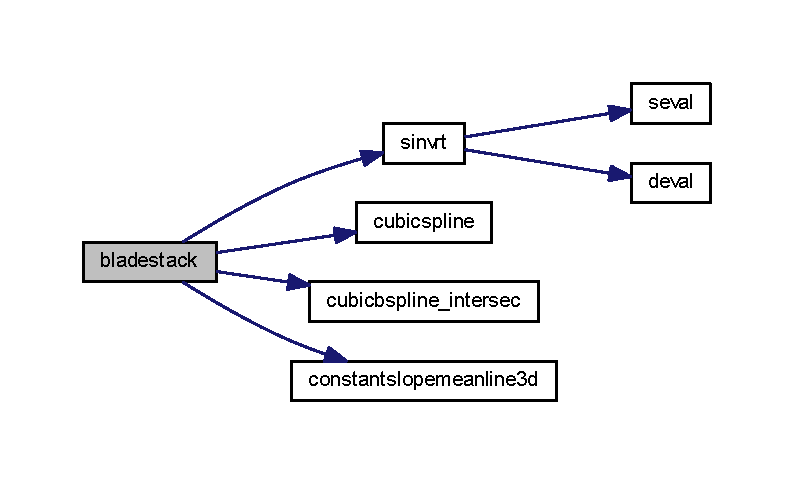
\includegraphics[width=350pt]{bladestack_8f90_a5dab74068855acf2e6917b70290ac7ec_cgraph}
\end{center}
\end{figure}




Here is the caller graph for this function\+:
\nopagebreak
\begin{figure}[H]
\begin{center}
\leavevmode
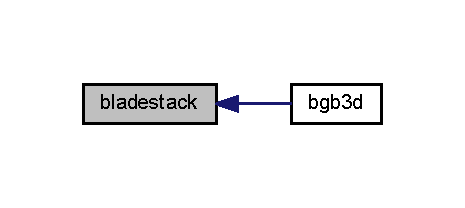
\includegraphics[width=223pt]{bladestack_8f90_a5dab74068855acf2e6917b70290ac7ec_icgraph}
\end{center}
\end{figure}



\hypertarget{bspline3_8f90}{}\section{C\+:/\+Git3\+D\+B\+G\+B/source/bspline3.f90 File Reference}
\label{bspline3_8f90}\index{C\+:/\+Git3\+D\+B\+G\+B/source/bspline3.\+f90@{C\+:/\+Git3\+D\+B\+G\+B/source/bspline3.\+f90}}
\subsection*{Functions/\+Subroutines}
\begin{DoxyCompactItemize}
\item 
subroutine \hyperlink{bspline3_8f90_a92250bb4e8b3cc6a081d56e982d5bfd7}{bspline3} (xcp, ycp, ncp, x, y, nspan, ia)
\item 
real $\ast$8 function \hyperlink{bspline3_8f90_a876b80c737790ddcd8cd93e9cf0c3d90}{bspline} (cp, t)
\item 
real $\ast$8 function \hyperlink{bspline3_8f90_a0a37f176ebc11541781e38f68f4d1a3e}{d\+\_\+bspline} (cp, t)
\item 
real $\ast$8 function \hyperlink{bspline3_8f90_a799109ca306b9e7ba96828dfb26a7608}{dd\+\_\+bspline} (cp, t)
\item 
real $\ast$8 function \hyperlink{bspline3_8f90_a0a51c311a84359ce64857be35fd49e26}{d3\+\_\+bspline} (cp, t)
\item 
subroutine \hyperlink{bspline3_8f90_a68f8db1f5c1e4f4e0784106fd195b1c0}{bspline\+\_\+arclength} (arclength, xcp, ycp, ncp, degree)
\item 
subroutine \hyperlink{bspline3_8f90_a4039b2d4eb7420c4db088018084c788e}{bspline\+\_\+jt} (j, t, arclength, ncp, degree, s)
\item 
real $\ast$8 function \hyperlink{bspline3_8f90_ad4747234d29e2a5f5b03a0093d9892cf}{bspline\+\_\+cp} (cp, arclength, ncp, degree, s)
\item 
real $\ast$8 function \hyperlink{bspline3_8f90_a8b69f577b0915d1c813ec5ef9f1d83e2}{d\+\_\+bspline\+\_\+cp} (cp, arclength, ncp, degree, s)
\item 
real $\ast$8 function \hyperlink{bspline3_8f90_aa631f1850271138144a5d22fc3399862}{dd\+\_\+bspline\+\_\+cp} (cp, arclength, ncp, degree, s)
\item 
real $\ast$8 function \hyperlink{bspline3_8f90_a4d0df1205efee4866b9e3c35eee96933}{d3\+\_\+bspline\+\_\+cp} (cp, arclength, ncp, degree, s)
\item 
real $\ast$8 function \hyperlink{bspline3_8f90_a30559a73ceea14913f355464954bb790}{d4\+\_\+bspline\+\_\+cp} (cp, arclength, ncp, degree, s)
\item 
subroutine \hyperlink{bspline3_8f90_ad414cab3eccec4d68ab800b9a676a921}{bspline\+\_\+y\+\_\+of\+\_\+x} (y, x, np, xcp, ycp, ncp, degree)
\item 
subroutine \hyperlink{bspline3_8f90_a7d2ef241d68f7850542865be9f217e5d}{bspline\+\_\+y\+\_\+of\+\_\+x\+\_\+refine} (y, x, np, xcp, ycp, ncp, degree)
\item 
real $\ast$8 function \hyperlink{bspline3_8f90_a47edcf85274770c2973d5ca6269e1c55}{bspline\+\_\+t\+\_\+newton} (cp, u)
\item 
real $\ast$8 function \hyperlink{bspline3_8f90_a32608cdb4f2dd2cddbcd585ea2e11622}{bspline4} (cp, t)
\item 
real $\ast$8 function \hyperlink{bspline3_8f90_aa5de7850f01068d93f8eb0c5890572e8}{d\+\_\+bspline4} (cp, t)
\item 
real $\ast$8 function \hyperlink{bspline3_8f90_aabbe2d5490d3ed9c6517877ff5148435}{dd\+\_\+bspline4} (cp, t)
\item 
real $\ast$8 function \hyperlink{bspline3_8f90_abc5eac4abfe9bd8a76820bc8e7a651f5}{d3\+\_\+bspline4} (cp, t)
\item 
real $\ast$8 function \hyperlink{bspline3_8f90_a6eb3c01da1c6fd0f74e36296f66746f4}{d4\+\_\+bspline4} (cp, t)
\item 
real $\ast$8 function \hyperlink{bspline3_8f90_a49900949e51d31c78d83ea2634d5bc8a}{bspline4\+\_\+t\+\_\+newton} (cp, u)
\end{DoxyCompactItemize}


\subsection{Function/\+Subroutine Documentation}
\hypertarget{bspline3_8f90_a876b80c737790ddcd8cd93e9cf0c3d90}{}\index{bspline3.\+f90@{bspline3.\+f90}!bspline@{bspline}}
\index{bspline@{bspline}!bspline3.\+f90@{bspline3.\+f90}}
\subsubsection[{bspline(cp, t)}]{\setlength{\rightskip}{0pt plus 5cm}real$\ast$8 function bspline (
\begin{DoxyParamCaption}
\item[{real$\ast$8, dimension(4), intent(in)}]{cp, }
\item[{real$\ast$8, intent(in)}]{t}
\end{DoxyParamCaption}
)}\label{bspline3_8f90_a876b80c737790ddcd8cd93e9cf0c3d90}
\hypertarget{bspline3_8f90_a92250bb4e8b3cc6a081d56e982d5bfd7}{}\index{bspline3.\+f90@{bspline3.\+f90}!bspline3@{bspline3}}
\index{bspline3@{bspline3}!bspline3.\+f90@{bspline3.\+f90}}
\subsubsection[{bspline3(xcp, ycp, ncp, x, y, nspan, ia)}]{\setlength{\rightskip}{0pt plus 5cm}subroutine bspline3 (
\begin{DoxyParamCaption}
\item[{real$\ast$8, dimension(ncp)}]{xcp, }
\item[{real$\ast$8, dimension(ncp)}]{ycp, }
\item[{integer}]{ncp, }
\item[{real$\ast$8, dimension(nspan)}]{x, }
\item[{real$\ast$8, dimension(nspan)}]{y, }
\item[{integer}]{nspan, }
\item[{integer}]{ia}
\end{DoxyParamCaption}
)}\label{bspline3_8f90_a92250bb4e8b3cc6a081d56e982d5bfd7}
\hypertarget{bspline3_8f90_a32608cdb4f2dd2cddbcd585ea2e11622}{}\index{bspline3.\+f90@{bspline3.\+f90}!bspline4@{bspline4}}
\index{bspline4@{bspline4}!bspline3.\+f90@{bspline3.\+f90}}
\subsubsection[{bspline4(cp, t)}]{\setlength{\rightskip}{0pt plus 5cm}real$\ast$8 function bspline4 (
\begin{DoxyParamCaption}
\item[{real$\ast$8, dimension(5), intent(in)}]{cp, }
\item[{real$\ast$8, intent(in)}]{t}
\end{DoxyParamCaption}
)}\label{bspline3_8f90_a32608cdb4f2dd2cddbcd585ea2e11622}
\hypertarget{bspline3_8f90_a49900949e51d31c78d83ea2634d5bc8a}{}\index{bspline3.\+f90@{bspline3.\+f90}!bspline4\+\_\+t\+\_\+newton@{bspline4\+\_\+t\+\_\+newton}}
\index{bspline4\+\_\+t\+\_\+newton@{bspline4\+\_\+t\+\_\+newton}!bspline3.\+f90@{bspline3.\+f90}}
\subsubsection[{bspline4\+\_\+t\+\_\+newton(cp, u)}]{\setlength{\rightskip}{0pt plus 5cm}real$\ast$8 function bspline4\+\_\+t\+\_\+newton (
\begin{DoxyParamCaption}
\item[{real$\ast$8, dimension(5), intent(in)}]{cp, }
\item[{real$\ast$8, intent(in)}]{u}
\end{DoxyParamCaption}
)}\label{bspline3_8f90_a49900949e51d31c78d83ea2634d5bc8a}
\hypertarget{bspline3_8f90_a68f8db1f5c1e4f4e0784106fd195b1c0}{}\index{bspline3.\+f90@{bspline3.\+f90}!bspline\+\_\+arclength@{bspline\+\_\+arclength}}
\index{bspline\+\_\+arclength@{bspline\+\_\+arclength}!bspline3.\+f90@{bspline3.\+f90}}
\subsubsection[{bspline\+\_\+arclength(arclength, xcp, ycp, ncp, degree)}]{\setlength{\rightskip}{0pt plus 5cm}subroutine bspline\+\_\+arclength (
\begin{DoxyParamCaption}
\item[{real$\ast$8, dimension(ncp-\/degree+1), intent(out)}]{arclength, }
\item[{real$\ast$8, dimension(ncp), intent(in)}]{xcp, }
\item[{real$\ast$8, dimension(ncp), intent(in)}]{ycp, }
\item[{integer, intent(in)}]{ncp, }
\item[{integer, intent(in)}]{degree}
\end{DoxyParamCaption}
)}\label{bspline3_8f90_a68f8db1f5c1e4f4e0784106fd195b1c0}


Here is the caller graph for this function\+:
\nopagebreak
\begin{figure}[H]
\begin{center}
\leavevmode
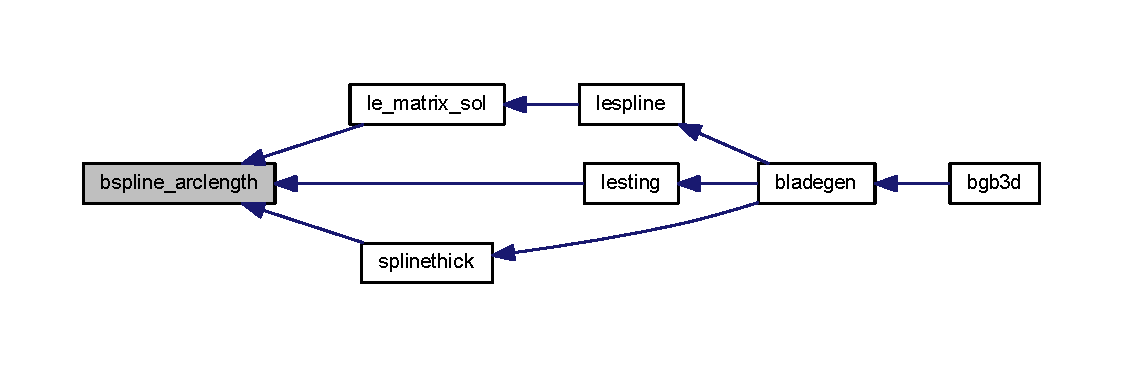
\includegraphics[width=350pt]{bspline3_8f90_a68f8db1f5c1e4f4e0784106fd195b1c0_icgraph}
\end{center}
\end{figure}


\hypertarget{bspline3_8f90_ad4747234d29e2a5f5b03a0093d9892cf}{}\index{bspline3.\+f90@{bspline3.\+f90}!bspline\+\_\+cp@{bspline\+\_\+cp}}
\index{bspline\+\_\+cp@{bspline\+\_\+cp}!bspline3.\+f90@{bspline3.\+f90}}
\subsubsection[{bspline\+\_\+cp(cp, arclength, ncp, degree, s)}]{\setlength{\rightskip}{0pt plus 5cm}real$\ast$8 function bspline\+\_\+cp (
\begin{DoxyParamCaption}
\item[{real$\ast$8, dimension(ncp), intent(in)}]{cp, }
\item[{real$\ast$8, dimension(ncp-\/2), intent(in)}]{arclength, }
\item[{integer, intent(in)}]{ncp, }
\item[{integer, intent(in)}]{degree, }
\item[{real$\ast$8, intent(in)}]{s}
\end{DoxyParamCaption}
)}\label{bspline3_8f90_ad4747234d29e2a5f5b03a0093d9892cf}


Here is the call graph for this function\+:
\nopagebreak
\begin{figure}[H]
\begin{center}
\leavevmode
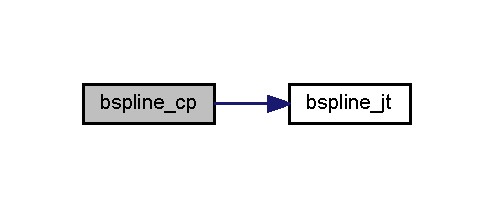
\includegraphics[width=237pt]{bspline3_8f90_ad4747234d29e2a5f5b03a0093d9892cf_cgraph}
\end{center}
\end{figure}


\hypertarget{bspline3_8f90_a4039b2d4eb7420c4db088018084c788e}{}\index{bspline3.\+f90@{bspline3.\+f90}!bspline\+\_\+jt@{bspline\+\_\+jt}}
\index{bspline\+\_\+jt@{bspline\+\_\+jt}!bspline3.\+f90@{bspline3.\+f90}}
\subsubsection[{bspline\+\_\+jt(j, t, arclength, ncp, degree, s)}]{\setlength{\rightskip}{0pt plus 5cm}subroutine bspline\+\_\+jt (
\begin{DoxyParamCaption}
\item[{integer, intent(out)}]{j, }
\item[{real$\ast$8, intent(out)}]{t, }
\item[{real$\ast$8, dimension(ncp-\/degree+1), intent(in)}]{arclength, }
\item[{integer, intent(in)}]{ncp, }
\item[{integer, intent(in)}]{degree, }
\item[{real$\ast$8, intent(in)}]{s}
\end{DoxyParamCaption}
)}\label{bspline3_8f90_a4039b2d4eb7420c4db088018084c788e}


Here is the caller graph for this function\+:
\nopagebreak
\begin{figure}[H]
\begin{center}
\leavevmode
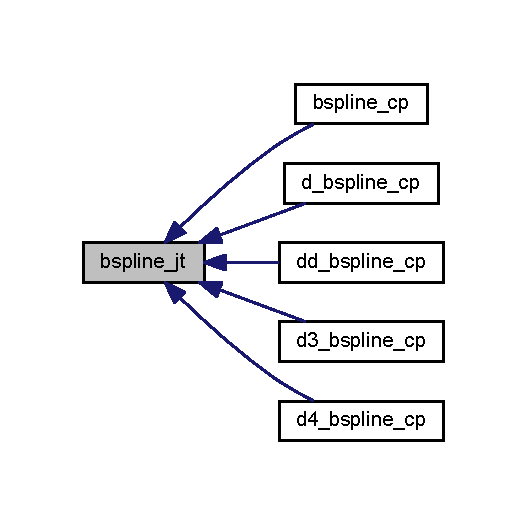
\includegraphics[width=253pt]{bspline3_8f90_a4039b2d4eb7420c4db088018084c788e_icgraph}
\end{center}
\end{figure}


\hypertarget{bspline3_8f90_a47edcf85274770c2973d5ca6269e1c55}{}\index{bspline3.\+f90@{bspline3.\+f90}!bspline\+\_\+t\+\_\+newton@{bspline\+\_\+t\+\_\+newton}}
\index{bspline\+\_\+t\+\_\+newton@{bspline\+\_\+t\+\_\+newton}!bspline3.\+f90@{bspline3.\+f90}}
\subsubsection[{bspline\+\_\+t\+\_\+newton(cp, u)}]{\setlength{\rightskip}{0pt plus 5cm}real$\ast$8 function bspline\+\_\+t\+\_\+newton (
\begin{DoxyParamCaption}
\item[{real$\ast$8, dimension(4), intent(in)}]{cp, }
\item[{real$\ast$8, intent(in)}]{u}
\end{DoxyParamCaption}
)}\label{bspline3_8f90_a47edcf85274770c2973d5ca6269e1c55}
\hypertarget{bspline3_8f90_ad414cab3eccec4d68ab800b9a676a921}{}\index{bspline3.\+f90@{bspline3.\+f90}!bspline\+\_\+y\+\_\+of\+\_\+x@{bspline\+\_\+y\+\_\+of\+\_\+x}}
\index{bspline\+\_\+y\+\_\+of\+\_\+x@{bspline\+\_\+y\+\_\+of\+\_\+x}!bspline3.\+f90@{bspline3.\+f90}}
\subsubsection[{bspline\+\_\+y\+\_\+of\+\_\+x(y, x, np, xcp, ycp, ncp, degree)}]{\setlength{\rightskip}{0pt plus 5cm}subroutine bspline\+\_\+y\+\_\+of\+\_\+x (
\begin{DoxyParamCaption}
\item[{real$\ast$8, dimension(np), intent(out)}]{y, }
\item[{real$\ast$8, dimension(np), intent(in)}]{x, }
\item[{integer, intent(in)}]{np, }
\item[{real$\ast$8, dimension(ncp), intent(in)}]{xcp, }
\item[{real$\ast$8, dimension(ncp), intent(in)}]{ycp, }
\item[{integer, intent(in)}]{ncp, }
\item[{integer, intent(in)}]{degree}
\end{DoxyParamCaption}
)}\label{bspline3_8f90_ad414cab3eccec4d68ab800b9a676a921}


Here is the caller graph for this function\+:
\nopagebreak
\begin{figure}[H]
\begin{center}
\leavevmode
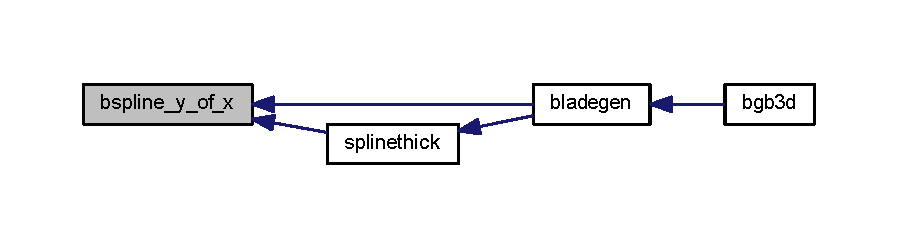
\includegraphics[width=350pt]{bspline3_8f90_ad414cab3eccec4d68ab800b9a676a921_icgraph}
\end{center}
\end{figure}


\hypertarget{bspline3_8f90_a7d2ef241d68f7850542865be9f217e5d}{}\index{bspline3.\+f90@{bspline3.\+f90}!bspline\+\_\+y\+\_\+of\+\_\+x\+\_\+refine@{bspline\+\_\+y\+\_\+of\+\_\+x\+\_\+refine}}
\index{bspline\+\_\+y\+\_\+of\+\_\+x\+\_\+refine@{bspline\+\_\+y\+\_\+of\+\_\+x\+\_\+refine}!bspline3.\+f90@{bspline3.\+f90}}
\subsubsection[{bspline\+\_\+y\+\_\+of\+\_\+x\+\_\+refine(y, x, np, xcp, ycp, ncp, degree)}]{\setlength{\rightskip}{0pt plus 5cm}subroutine bspline\+\_\+y\+\_\+of\+\_\+x\+\_\+refine (
\begin{DoxyParamCaption}
\item[{real$\ast$8, dimension(np), intent(out)}]{y, }
\item[{real$\ast$8, dimension(np), intent(in)}]{x, }
\item[{integer, intent(in)}]{np, }
\item[{real$\ast$8, dimension(ncp), intent(in)}]{xcp, }
\item[{real$\ast$8, dimension(ncp), intent(in)}]{ycp, }
\item[{integer, intent(in)}]{ncp, }
\item[{integer, intent(in)}]{degree}
\end{DoxyParamCaption}
)}\label{bspline3_8f90_a7d2ef241d68f7850542865be9f217e5d}


Here is the caller graph for this function\+:
\nopagebreak
\begin{figure}[H]
\begin{center}
\leavevmode
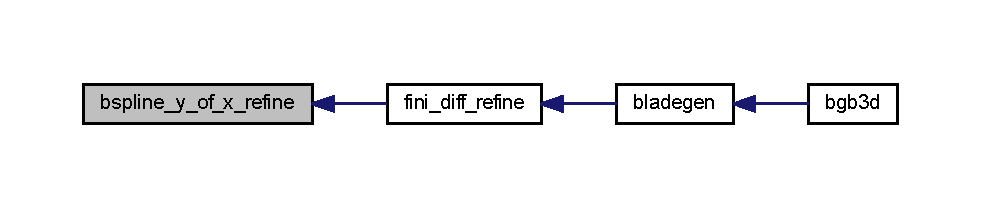
\includegraphics[width=350pt]{bspline3_8f90_a7d2ef241d68f7850542865be9f217e5d_icgraph}
\end{center}
\end{figure}


\hypertarget{bspline3_8f90_a0a51c311a84359ce64857be35fd49e26}{}\index{bspline3.\+f90@{bspline3.\+f90}!d3\+\_\+bspline@{d3\+\_\+bspline}}
\index{d3\+\_\+bspline@{d3\+\_\+bspline}!bspline3.\+f90@{bspline3.\+f90}}
\subsubsection[{d3\+\_\+bspline(cp, t)}]{\setlength{\rightskip}{0pt plus 5cm}real$\ast$8 function d3\+\_\+bspline (
\begin{DoxyParamCaption}
\item[{real$\ast$8, dimension(4), intent(in)}]{cp, }
\item[{real$\ast$8, intent(in)}]{t}
\end{DoxyParamCaption}
)}\label{bspline3_8f90_a0a51c311a84359ce64857be35fd49e26}
\hypertarget{bspline3_8f90_abc5eac4abfe9bd8a76820bc8e7a651f5}{}\index{bspline3.\+f90@{bspline3.\+f90}!d3\+\_\+bspline4@{d3\+\_\+bspline4}}
\index{d3\+\_\+bspline4@{d3\+\_\+bspline4}!bspline3.\+f90@{bspline3.\+f90}}
\subsubsection[{d3\+\_\+bspline4(cp, t)}]{\setlength{\rightskip}{0pt plus 5cm}real$\ast$8 function d3\+\_\+bspline4 (
\begin{DoxyParamCaption}
\item[{real$\ast$8, dimension(5), intent(in)}]{cp, }
\item[{real$\ast$8, intent(in)}]{t}
\end{DoxyParamCaption}
)}\label{bspline3_8f90_abc5eac4abfe9bd8a76820bc8e7a651f5}
\hypertarget{bspline3_8f90_a4d0df1205efee4866b9e3c35eee96933}{}\index{bspline3.\+f90@{bspline3.\+f90}!d3\+\_\+bspline\+\_\+cp@{d3\+\_\+bspline\+\_\+cp}}
\index{d3\+\_\+bspline\+\_\+cp@{d3\+\_\+bspline\+\_\+cp}!bspline3.\+f90@{bspline3.\+f90}}
\subsubsection[{d3\+\_\+bspline\+\_\+cp(cp, arclength, ncp, degree, s)}]{\setlength{\rightskip}{0pt plus 5cm}real$\ast$8 function d3\+\_\+bspline\+\_\+cp (
\begin{DoxyParamCaption}
\item[{real$\ast$8, dimension(ncp), intent(in)}]{cp, }
\item[{real$\ast$8, dimension(ncp-\/2), intent(in)}]{arclength, }
\item[{integer, intent(in)}]{ncp, }
\item[{integer, intent(in)}]{degree, }
\item[{real$\ast$8, intent(in)}]{s}
\end{DoxyParamCaption}
)}\label{bspline3_8f90_a4d0df1205efee4866b9e3c35eee96933}


Here is the call graph for this function\+:
\nopagebreak
\begin{figure}[H]
\begin{center}
\leavevmode
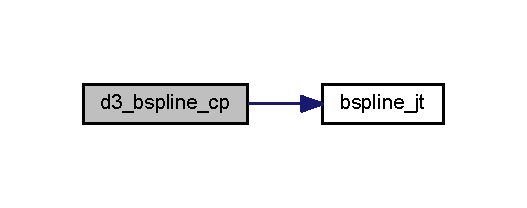
\includegraphics[width=253pt]{bspline3_8f90_a4d0df1205efee4866b9e3c35eee96933_cgraph}
\end{center}
\end{figure}


\hypertarget{bspline3_8f90_a6eb3c01da1c6fd0f74e36296f66746f4}{}\index{bspline3.\+f90@{bspline3.\+f90}!d4\+\_\+bspline4@{d4\+\_\+bspline4}}
\index{d4\+\_\+bspline4@{d4\+\_\+bspline4}!bspline3.\+f90@{bspline3.\+f90}}
\subsubsection[{d4\+\_\+bspline4(cp, t)}]{\setlength{\rightskip}{0pt plus 5cm}real$\ast$8 function d4\+\_\+bspline4 (
\begin{DoxyParamCaption}
\item[{real$\ast$8, dimension(5), intent(in)}]{cp, }
\item[{real$\ast$8, intent(in)}]{t}
\end{DoxyParamCaption}
)}\label{bspline3_8f90_a6eb3c01da1c6fd0f74e36296f66746f4}
\hypertarget{bspline3_8f90_a30559a73ceea14913f355464954bb790}{}\index{bspline3.\+f90@{bspline3.\+f90}!d4\+\_\+bspline\+\_\+cp@{d4\+\_\+bspline\+\_\+cp}}
\index{d4\+\_\+bspline\+\_\+cp@{d4\+\_\+bspline\+\_\+cp}!bspline3.\+f90@{bspline3.\+f90}}
\subsubsection[{d4\+\_\+bspline\+\_\+cp(cp, arclength, ncp, degree, s)}]{\setlength{\rightskip}{0pt plus 5cm}real$\ast$8 function d4\+\_\+bspline\+\_\+cp (
\begin{DoxyParamCaption}
\item[{real$\ast$8, dimension(ncp), intent(in)}]{cp, }
\item[{real$\ast$8, dimension(ncp-\/2), intent(in)}]{arclength, }
\item[{integer, intent(in)}]{ncp, }
\item[{integer, intent(in)}]{degree, }
\item[{real$\ast$8, intent(in)}]{s}
\end{DoxyParamCaption}
)}\label{bspline3_8f90_a30559a73ceea14913f355464954bb790}


Here is the call graph for this function\+:
\nopagebreak
\begin{figure}[H]
\begin{center}
\leavevmode
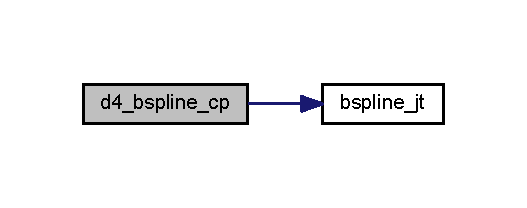
\includegraphics[width=253pt]{bspline3_8f90_a30559a73ceea14913f355464954bb790_cgraph}
\end{center}
\end{figure}


\hypertarget{bspline3_8f90_a0a37f176ebc11541781e38f68f4d1a3e}{}\index{bspline3.\+f90@{bspline3.\+f90}!d\+\_\+bspline@{d\+\_\+bspline}}
\index{d\+\_\+bspline@{d\+\_\+bspline}!bspline3.\+f90@{bspline3.\+f90}}
\subsubsection[{d\+\_\+bspline(cp, t)}]{\setlength{\rightskip}{0pt plus 5cm}real$\ast$8 function d\+\_\+bspline (
\begin{DoxyParamCaption}
\item[{real$\ast$8, dimension(4), intent(in)}]{cp, }
\item[{real$\ast$8, intent(in)}]{t}
\end{DoxyParamCaption}
)}\label{bspline3_8f90_a0a37f176ebc11541781e38f68f4d1a3e}
\hypertarget{bspline3_8f90_aa5de7850f01068d93f8eb0c5890572e8}{}\index{bspline3.\+f90@{bspline3.\+f90}!d\+\_\+bspline4@{d\+\_\+bspline4}}
\index{d\+\_\+bspline4@{d\+\_\+bspline4}!bspline3.\+f90@{bspline3.\+f90}}
\subsubsection[{d\+\_\+bspline4(cp, t)}]{\setlength{\rightskip}{0pt plus 5cm}real$\ast$8 function d\+\_\+bspline4 (
\begin{DoxyParamCaption}
\item[{real$\ast$8, dimension(5), intent(in)}]{cp, }
\item[{real$\ast$8, intent(in)}]{t}
\end{DoxyParamCaption}
)}\label{bspline3_8f90_aa5de7850f01068d93f8eb0c5890572e8}
\hypertarget{bspline3_8f90_a8b69f577b0915d1c813ec5ef9f1d83e2}{}\index{bspline3.\+f90@{bspline3.\+f90}!d\+\_\+bspline\+\_\+cp@{d\+\_\+bspline\+\_\+cp}}
\index{d\+\_\+bspline\+\_\+cp@{d\+\_\+bspline\+\_\+cp}!bspline3.\+f90@{bspline3.\+f90}}
\subsubsection[{d\+\_\+bspline\+\_\+cp(cp, arclength, ncp, degree, s)}]{\setlength{\rightskip}{0pt plus 5cm}real$\ast$8 function d\+\_\+bspline\+\_\+cp (
\begin{DoxyParamCaption}
\item[{real$\ast$8, dimension(ncp), intent(in)}]{cp, }
\item[{real$\ast$8, dimension(ncp-\/2), intent(in)}]{arclength, }
\item[{integer, intent(in)}]{ncp, }
\item[{integer, intent(in)}]{degree, }
\item[{real$\ast$8, intent(in)}]{s}
\end{DoxyParamCaption}
)}\label{bspline3_8f90_a8b69f577b0915d1c813ec5ef9f1d83e2}


Here is the call graph for this function\+:
\nopagebreak
\begin{figure}[H]
\begin{center}
\leavevmode
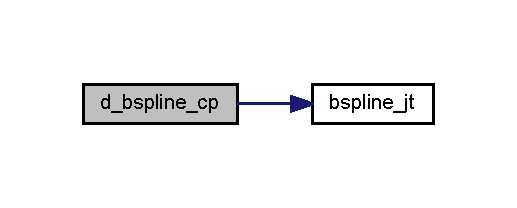
\includegraphics[width=248pt]{bspline3_8f90_a8b69f577b0915d1c813ec5ef9f1d83e2_cgraph}
\end{center}
\end{figure}


\hypertarget{bspline3_8f90_a799109ca306b9e7ba96828dfb26a7608}{}\index{bspline3.\+f90@{bspline3.\+f90}!dd\+\_\+bspline@{dd\+\_\+bspline}}
\index{dd\+\_\+bspline@{dd\+\_\+bspline}!bspline3.\+f90@{bspline3.\+f90}}
\subsubsection[{dd\+\_\+bspline(cp, t)}]{\setlength{\rightskip}{0pt plus 5cm}real$\ast$8 function dd\+\_\+bspline (
\begin{DoxyParamCaption}
\item[{real$\ast$8, dimension(4), intent(in)}]{cp, }
\item[{real$\ast$8, intent(in)}]{t}
\end{DoxyParamCaption}
)}\label{bspline3_8f90_a799109ca306b9e7ba96828dfb26a7608}
\hypertarget{bspline3_8f90_aabbe2d5490d3ed9c6517877ff5148435}{}\index{bspline3.\+f90@{bspline3.\+f90}!dd\+\_\+bspline4@{dd\+\_\+bspline4}}
\index{dd\+\_\+bspline4@{dd\+\_\+bspline4}!bspline3.\+f90@{bspline3.\+f90}}
\subsubsection[{dd\+\_\+bspline4(cp, t)}]{\setlength{\rightskip}{0pt plus 5cm}real$\ast$8 function dd\+\_\+bspline4 (
\begin{DoxyParamCaption}
\item[{real$\ast$8, dimension(5), intent(in)}]{cp, }
\item[{real$\ast$8, intent(in)}]{t}
\end{DoxyParamCaption}
)}\label{bspline3_8f90_aabbe2d5490d3ed9c6517877ff5148435}
\hypertarget{bspline3_8f90_aa631f1850271138144a5d22fc3399862}{}\index{bspline3.\+f90@{bspline3.\+f90}!dd\+\_\+bspline\+\_\+cp@{dd\+\_\+bspline\+\_\+cp}}
\index{dd\+\_\+bspline\+\_\+cp@{dd\+\_\+bspline\+\_\+cp}!bspline3.\+f90@{bspline3.\+f90}}
\subsubsection[{dd\+\_\+bspline\+\_\+cp(cp, arclength, ncp, degree, s)}]{\setlength{\rightskip}{0pt plus 5cm}real$\ast$8 function dd\+\_\+bspline\+\_\+cp (
\begin{DoxyParamCaption}
\item[{real$\ast$8, dimension(ncp), intent(in)}]{cp, }
\item[{real$\ast$8, dimension(ncp-\/2), intent(in)}]{arclength, }
\item[{integer, intent(in)}]{ncp, }
\item[{integer, intent(in)}]{degree, }
\item[{real$\ast$8, intent(in)}]{s}
\end{DoxyParamCaption}
)}\label{bspline3_8f90_aa631f1850271138144a5d22fc3399862}


Here is the call graph for this function\+:
\nopagebreak
\begin{figure}[H]
\begin{center}
\leavevmode
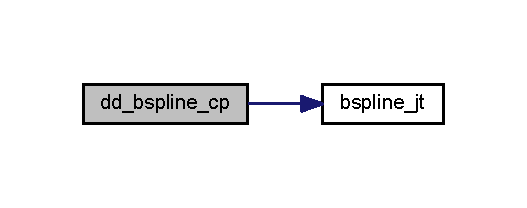
\includegraphics[width=253pt]{bspline3_8f90_aa631f1850271138144a5d22fc3399862_cgraph}
\end{center}
\end{figure}



\hypertarget{bsplinecam_8f90}{}\section{C\+:/\+Git3\+D\+B\+G\+B/source/bsplinecam.f90 File Reference}
\label{bsplinecam_8f90}\index{C\+:/\+Git3\+D\+B\+G\+B/source/bsplinecam.\+f90@{C\+:/\+Git3\+D\+B\+G\+B/source/bsplinecam.\+f90}}
\subsection*{Functions/\+Subroutines}
\begin{DoxyCompactItemize}
\item 
subroutine \hyperlink{bsplinecam_8f90_a9b1c34e73d6eb153d605e06274effdae}{bsplinecam} (xcp, ycp, np, ncp, u, ainl, aext, sang, chrd, cam\+\_\+u, c
\item 
real $\ast$8 function \hyperlink{bsplinecam_8f90_af4379365bf9e92538191fcb377a6e7fa}{angle} (y\+\_\+cp, x\+\_\+cp, angle0, t)
\item 
real $\ast$8 function \hyperlink{bsplinecam_8f90_a5f344dd1ac7aa0679039a2bd0531aec6}{camber} (y\+\_\+cp, x\+\_\+cp, angle0, camber0, t)
\end{DoxyCompactItemize}


\subsection{Function/\+Subroutine Documentation}
\hypertarget{bsplinecam_8f90_af4379365bf9e92538191fcb377a6e7fa}{}\index{bsplinecam.\+f90@{bsplinecam.\+f90}!angle@{angle}}
\index{angle@{angle}!bsplinecam.\+f90@{bsplinecam.\+f90}}
\subsubsection[{angle(y\+\_\+cp, x\+\_\+cp, angle0, t)}]{\setlength{\rightskip}{0pt plus 5cm}real$\ast$8 function angle (
\begin{DoxyParamCaption}
\item[{real$\ast$8, dimension(4), intent(in)}]{y\+\_\+cp, }
\item[{real$\ast$8, dimension(4), intent(in)}]{x\+\_\+cp, }
\item[{real$\ast$8, intent(in)}]{angle0, }
\item[{real$\ast$8, intent(in)}]{t}
\end{DoxyParamCaption}
)}\label{bsplinecam_8f90_af4379365bf9e92538191fcb377a6e7fa}


Here is the caller graph for this function\+:
\nopagebreak
\begin{figure}[H]
\begin{center}
\leavevmode
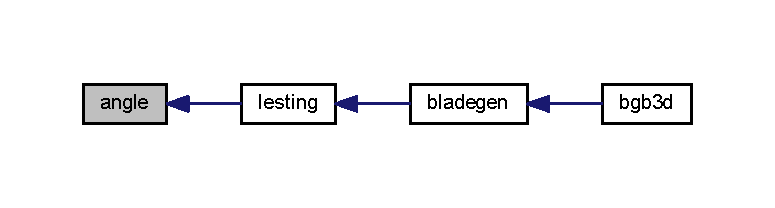
\includegraphics[width=350pt]{bsplinecam_8f90_af4379365bf9e92538191fcb377a6e7fa_icgraph}
\end{center}
\end{figure}


\hypertarget{bsplinecam_8f90_a9b1c34e73d6eb153d605e06274effdae}{}\index{bsplinecam.\+f90@{bsplinecam.\+f90}!bsplinecam@{bsplinecam}}
\index{bsplinecam@{bsplinecam}!bsplinecam.\+f90@{bsplinecam.\+f90}}
\subsubsection[{bsplinecam(xcp, ycp, np, ncp, u, ainl, aext, sang, chrd, cam\+\_\+u, c}]{\setlength{\rightskip}{0pt plus 5cm}subroutine bsplinecam (
\begin{DoxyParamCaption}
\item[{real$\ast$8, dimension(ncp)}]{xcp, }
\item[{real$\ast$8, dimension(ncp)}]{ycp, }
\item[{integer}]{np, }
\item[{integer}]{ncp, }
\item[{real$\ast$8, dimension(np\+\_\+side)}]{u, }
\item[{real$\ast$8}]{ainl, }
\item[{real$\ast$8}]{aext, }
\item[{real$\ast$8}]{sang, }
\item[{real$\ast$8}]{chrd, }
\item[{real$\ast$8, dimension(np)}]{cam\+\_\+u, }
\item[{}]{c}
\end{DoxyParamCaption}
)}\label{bsplinecam_8f90_a9b1c34e73d6eb153d605e06274effdae}


Here is the caller graph for this function\+:
\nopagebreak
\begin{figure}[H]
\begin{center}
\leavevmode
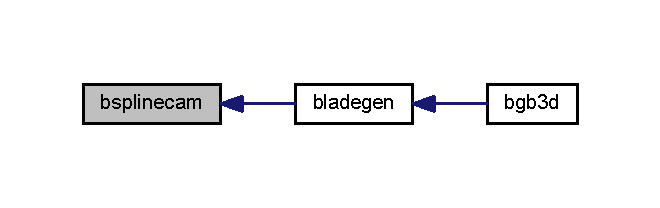
\includegraphics[width=317pt]{bsplinecam_8f90_a9b1c34e73d6eb153d605e06274effdae_icgraph}
\end{center}
\end{figure}


\hypertarget{bsplinecam_8f90_a5f344dd1ac7aa0679039a2bd0531aec6}{}\index{bsplinecam.\+f90@{bsplinecam.\+f90}!camber@{camber}}
\index{camber@{camber}!bsplinecam.\+f90@{bsplinecam.\+f90}}
\subsubsection[{camber(y\+\_\+cp, x\+\_\+cp, angle0, camber0, t)}]{\setlength{\rightskip}{0pt plus 5cm}real$\ast$8 function camber (
\begin{DoxyParamCaption}
\item[{real$\ast$8, dimension(4), intent(in)}]{y\+\_\+cp, }
\item[{real$\ast$8, dimension(4), intent(in)}]{x\+\_\+cp, }
\item[{real$\ast$8, intent(in)}]{angle0, }
\item[{real$\ast$8, intent(in)}]{camber0, }
\item[{real$\ast$8, intent(in)}]{t}
\end{DoxyParamCaption}
)}\label{bsplinecam_8f90_a5f344dd1ac7aa0679039a2bd0531aec6}


Here is the caller graph for this function\+:
\nopagebreak
\begin{figure}[H]
\begin{center}
\leavevmode
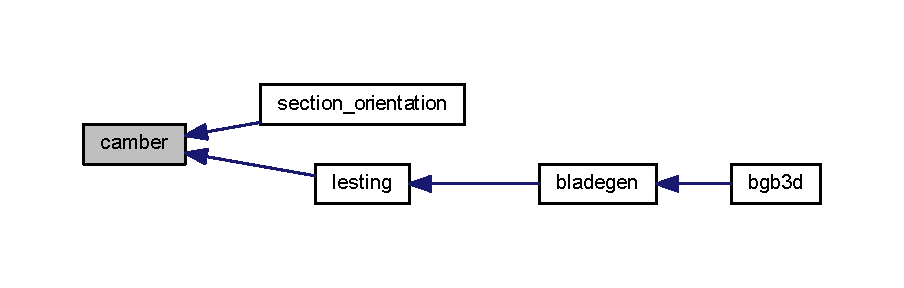
\includegraphics[width=350pt]{bsplinecam_8f90_a5f344dd1ac7aa0679039a2bd0531aec6_icgraph}
\end{center}
\end{figure}



\hypertarget{cubicspline_8f90}{}\section{C\+:/\+Git3\+D\+B\+G\+B/source/cubicspline.f90 File Reference}
\label{cubicspline_8f90}\index{C\+:/\+Git3\+D\+B\+G\+B/source/cubicspline.\+f90@{C\+:/\+Git3\+D\+B\+G\+B/source/cubicspline.\+f90}}
\subsection*{Functions/\+Subroutines}
\begin{DoxyCompactItemize}
\item 
subroutine \hyperlink{cubicspline_8f90_a0d7ea172c4dd062e3e0cc2a4dc93a5b3}{cubicspline} (xcp, ycp, ncp, xbs, ybs, y\+\_\+spl\+\_\+end, nspline, xc, yc, ncp1)
\item 
subroutine \hyperlink{cubicspline_8f90_accb11d22a494402144708cfd257358c9}{curv\+\_\+line\+\_\+inters} (xbs, ybs, nspline, xin, yout, nspan)
\item 
subroutine \hyperlink{cubicspline_8f90_aa5112970664c428d0eb49a8a8345adab}{curvline\+\_\+intersec} (xcp, ycp, ncp, xinarray, youtarray, na, ia)
\item 
subroutine \hyperlink{cubicspline_8f90_a61e3967b950c5647c24960902402617b}{cubicbspline\+\_\+intersec} (y\+\_\+spl\+\_\+end, xcp, ycp, ncp, xin, yout, na, xbs, ybs)
\item 
subroutine \hyperlink{cubicspline_8f90_aa8e12bbf7fdbab334fce7dc8a67c9d5c}{cubicbspline} (ncp, ncp1, np, cp, cbs)
\end{DoxyCompactItemize}


\subsection{Function/\+Subroutine Documentation}
\hypertarget{cubicspline_8f90_aa8e12bbf7fdbab334fce7dc8a67c9d5c}{}\index{cubicspline.\+f90@{cubicspline.\+f90}!cubicbspline@{cubicbspline}}
\index{cubicbspline@{cubicbspline}!cubicspline.\+f90@{cubicspline.\+f90}}
\subsubsection[{cubicbspline(ncp, ncp1, np, cp, cbs)}]{\setlength{\rightskip}{0pt plus 5cm}subroutine cubicbspline (
\begin{DoxyParamCaption}
\item[{integer}]{ncp, }
\item[{integer}]{ncp1, }
\item[{integer}]{np, }
\item[{real$\ast$8, dimension(ncp)}]{cp, }
\item[{real$\ast$8, dimension(np$\ast$(ncp1-\/3))}]{cbs}
\end{DoxyParamCaption}
)}\label{cubicspline_8f90_aa8e12bbf7fdbab334fce7dc8a67c9d5c}


Here is the caller graph for this function\+:
\nopagebreak
\begin{figure}[H]
\begin{center}
\leavevmode
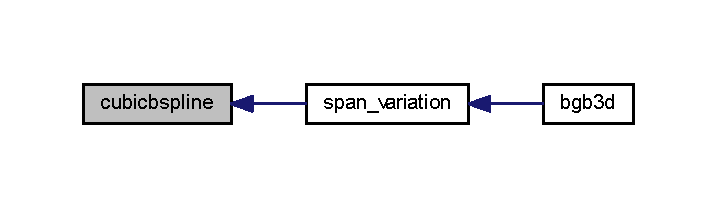
\includegraphics[width=344pt]{cubicspline_8f90_aa8e12bbf7fdbab334fce7dc8a67c9d5c_icgraph}
\end{center}
\end{figure}


\hypertarget{cubicspline_8f90_a61e3967b950c5647c24960902402617b}{}\index{cubicspline.\+f90@{cubicspline.\+f90}!cubicbspline\+\_\+intersec@{cubicbspline\+\_\+intersec}}
\index{cubicbspline\+\_\+intersec@{cubicbspline\+\_\+intersec}!cubicspline.\+f90@{cubicspline.\+f90}}
\subsubsection[{cubicbspline\+\_\+intersec(y\+\_\+spl\+\_\+end, xcp, ycp, ncp, xin, yout, na, xbs, ybs)}]{\setlength{\rightskip}{0pt plus 5cm}subroutine cubicbspline\+\_\+intersec (
\begin{DoxyParamCaption}
\item[{real$\ast$8, dimension(ncp-\/2)}]{y\+\_\+spl\+\_\+end, }
\item[{real$\ast$8, dimension(ncp)}]{xcp, }
\item[{real$\ast$8, dimension(ncp)}]{ycp, }
\item[{integer}]{ncp, }
\item[{real$\ast$8, dimension(na)}]{xin, }
\item[{real$\ast$8, dimension(na)}]{yout, }
\item[{integer}]{na, }
\item[{real$\ast$8, dimension(np$\ast$(ncp-\/3))}]{xbs, }
\item[{real$\ast$8, dimension(np$\ast$(ncp-\/3))}]{ybs}
\end{DoxyParamCaption}
)}\label{cubicspline_8f90_a61e3967b950c5647c24960902402617b}


Here is the caller graph for this function\+:
\nopagebreak
\begin{figure}[H]
\begin{center}
\leavevmode
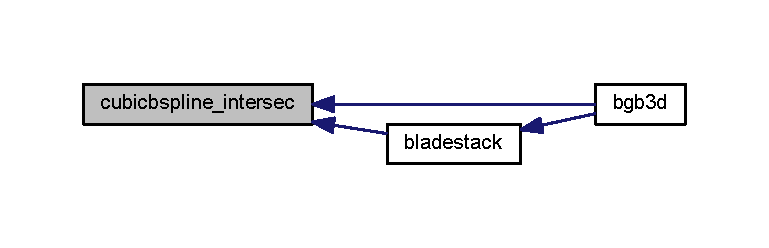
\includegraphics[width=350pt]{cubicspline_8f90_a61e3967b950c5647c24960902402617b_icgraph}
\end{center}
\end{figure}


\hypertarget{cubicspline_8f90_a0d7ea172c4dd062e3e0cc2a4dc93a5b3}{}\index{cubicspline.\+f90@{cubicspline.\+f90}!cubicspline@{cubicspline}}
\index{cubicspline@{cubicspline}!cubicspline.\+f90@{cubicspline.\+f90}}
\subsubsection[{cubicspline(xcp, ycp, ncp, xbs, ybs, y\+\_\+spl\+\_\+end, nspline, xc, yc, ncp1)}]{\setlength{\rightskip}{0pt plus 5cm}subroutine cubicspline (
\begin{DoxyParamCaption}
\item[{real$\ast$8, dimension(ncp)}]{xcp, }
\item[{real$\ast$8, dimension(ncp)}]{ycp, }
\item[{integer}]{ncp, }
\item[{real$\ast$8, dimension(nx)}]{xbs, }
\item[{real$\ast$8, dimension(nx)}]{ybs, }
\item[{real$\ast$8, dimension(ncp)}]{y\+\_\+spl\+\_\+end, }
\item[{integer}]{nspline, }
\item[{real$\ast$8, dimension(ncp+2)}]{xc, }
\item[{real$\ast$8, dimension(ncp+2)}]{yc, }
\item[{integer}]{ncp1}
\end{DoxyParamCaption}
)}\label{cubicspline_8f90_a0d7ea172c4dd062e3e0cc2a4dc93a5b3}


Here is the caller graph for this function\+:
\nopagebreak
\begin{figure}[H]
\begin{center}
\leavevmode
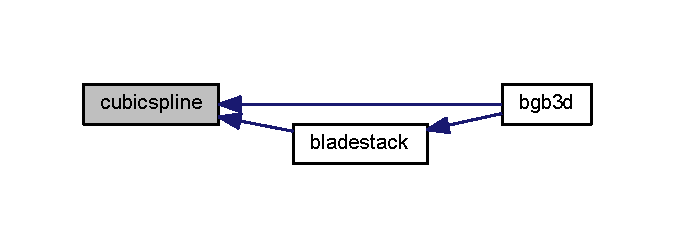
\includegraphics[width=324pt]{cubicspline_8f90_a0d7ea172c4dd062e3e0cc2a4dc93a5b3_icgraph}
\end{center}
\end{figure}


\hypertarget{cubicspline_8f90_accb11d22a494402144708cfd257358c9}{}\index{cubicspline.\+f90@{cubicspline.\+f90}!curv\+\_\+line\+\_\+inters@{curv\+\_\+line\+\_\+inters}}
\index{curv\+\_\+line\+\_\+inters@{curv\+\_\+line\+\_\+inters}!cubicspline.\+f90@{cubicspline.\+f90}}
\subsubsection[{curv\+\_\+line\+\_\+inters(xbs, ybs, nspline, xin, yout, nspan)}]{\setlength{\rightskip}{0pt plus 5cm}subroutine curv\+\_\+line\+\_\+inters (
\begin{DoxyParamCaption}
\item[{real$\ast$8, dimension(nspline)}]{xbs, }
\item[{real$\ast$8, dimension(nspline)}]{ybs, }
\item[{integer}]{nspline, }
\item[{real$\ast$8, dimension(nspan)}]{xin, }
\item[{real$\ast$8, dimension(nspan)}]{yout, }
\item[{integer}]{nspan}
\end{DoxyParamCaption}
)}\label{cubicspline_8f90_accb11d22a494402144708cfd257358c9}


Here is the caller graph for this function\+:
\nopagebreak
\begin{figure}[H]
\begin{center}
\leavevmode
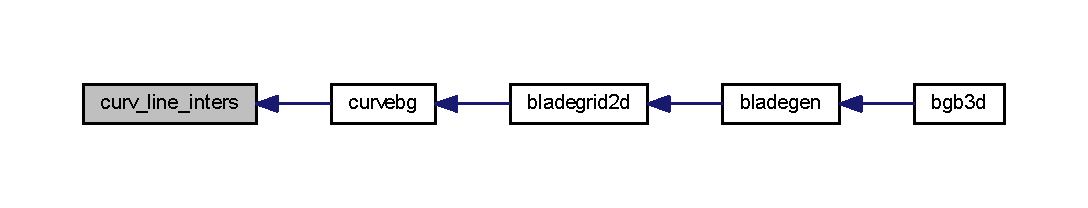
\includegraphics[width=350pt]{cubicspline_8f90_accb11d22a494402144708cfd257358c9_icgraph}
\end{center}
\end{figure}


\hypertarget{cubicspline_8f90_aa5112970664c428d0eb49a8a8345adab}{}\index{cubicspline.\+f90@{cubicspline.\+f90}!curvline\+\_\+intersec@{curvline\+\_\+intersec}}
\index{curvline\+\_\+intersec@{curvline\+\_\+intersec}!cubicspline.\+f90@{cubicspline.\+f90}}
\subsubsection[{curvline\+\_\+intersec(xcp, ycp, ncp, xinarray, youtarray, na, ia)}]{\setlength{\rightskip}{0pt plus 5cm}subroutine curvline\+\_\+intersec (
\begin{DoxyParamCaption}
\item[{real$\ast$8, dimension(ncp)}]{xcp, }
\item[{real$\ast$8, dimension(ncp)}]{ycp, }
\item[{integer}]{ncp, }
\item[{real$\ast$8, dimension(na)}]{xinarray, }
\item[{real$\ast$8, dimension(na)}]{youtarray, }
\item[{integer}]{na, }
\item[{integer}]{ia}
\end{DoxyParamCaption}
)}\label{cubicspline_8f90_aa5112970664c428d0eb49a8a8345adab}

\hypertarget{dmat__solve_8f90}{}\section{C\+:/\+Git3\+D\+B\+G\+B/source/dmat\+\_\+solve.f90 File Reference}
\label{dmat__solve_8f90}\index{C\+:/\+Git3\+D\+B\+G\+B/source/dmat\+\_\+solve.\+f90@{C\+:/\+Git3\+D\+B\+G\+B/source/dmat\+\_\+solve.\+f90}}
\subsection*{Functions/\+Subroutines}
\begin{DoxyCompactItemize}
\item 
subroutine \hyperlink{dmat__solve_8f90_ad79706b7f3c6b3339baccb3a798e9a92}{dmat\+\_\+solve} (n, nrhs, a, info)
\end{DoxyCompactItemize}


\subsection{Function/\+Subroutine Documentation}
\hypertarget{dmat__solve_8f90_ad79706b7f3c6b3339baccb3a798e9a92}{}\index{dmat\+\_\+solve.\+f90@{dmat\+\_\+solve.\+f90}!dmat\+\_\+solve@{dmat\+\_\+solve}}
\index{dmat\+\_\+solve@{dmat\+\_\+solve}!dmat\+\_\+solve.\+f90@{dmat\+\_\+solve.\+f90}}
\subsubsection[{dmat\+\_\+solve(n, nrhs, a, info)}]{\setlength{\rightskip}{0pt plus 5cm}subroutine dmat\+\_\+solve (
\begin{DoxyParamCaption}
\item[{integer}]{n, }
\item[{integer}]{nrhs, }
\item[{real ( kind = 8 ), dimension(n,n+nrhs)}]{a, }
\item[{integer}]{info}
\end{DoxyParamCaption}
)}\label{dmat__solve_8f90_ad79706b7f3c6b3339baccb3a798e9a92}


Here is the caller graph for this function\+:
\nopagebreak
\begin{figure}[H]
\begin{center}
\leavevmode
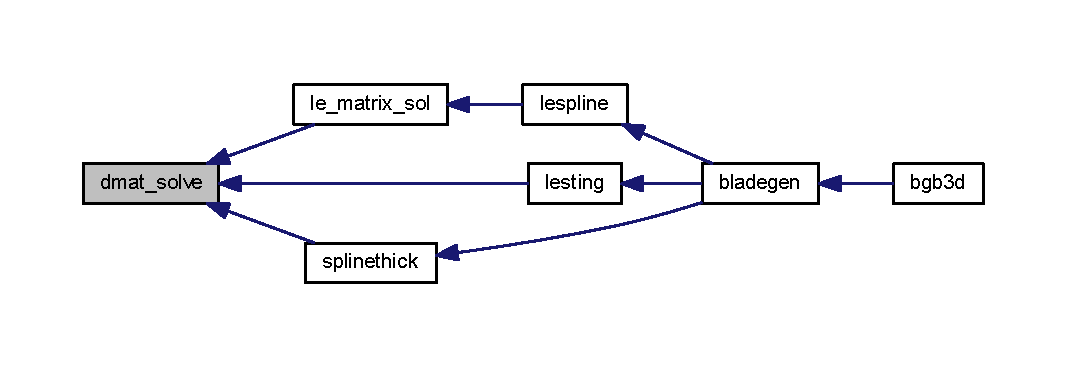
\includegraphics[width=350pt]{dmat__solve_8f90_ad79706b7f3c6b3339baccb3a798e9a92_icgraph}
\end{center}
\end{figure}



\hypertarget{ellipgrid_8f90}{}\section{C\+:/\+Git3\+D\+B\+G\+B/source/ellipgrid.f90 File Reference}
\label{ellipgrid_8f90}\index{C\+:/\+Git3\+D\+B\+G\+B/source/ellipgrid.\+f90@{C\+:/\+Git3\+D\+B\+G\+B/source/ellipgrid.\+f90}}
\subsection*{Functions/\+Subroutines}
\begin{DoxyCompactItemize}
\item 
subroutine \hyperlink{ellipgrid_8f90_ad37e0a5511289684f99d62342ff71a68}{gausei2d} (ni, nj, x, y, err, curvemesh, ellipsmooth)
\item 
subroutine \hyperlink{ellipgrid_8f90_a9700874d36140d2c7bee117590d5dae9}{gausei2dblade} (ni, nj, x, y, err, curvemesh, ellipsmooth, L\+E)
\item 
subroutine \hyperlink{ellipgrid_8f90_adefdbbd93b3c42f5c88bf066fffda020}{curvebg} (imax, jmax, xblade, yblade,                                                                               uplmt, np, casename, develop, isdev, msle, mble, chrd, pitch)
\item 
subroutine \hyperlink{ellipgrid_8f90_a23f0130faf07695ae0633d37888c9298}{linearbg} (imax, jmax, xblade, yblade,                                               uplmt, np, casename, develop, msle, mble, chrd, pitch)
\item 
subroutine \hyperlink{ellipgrid_8f90_ae47ef85c421748bee190d8cffa59a6cf}{stinglegrid} (xb, yb, np, uplmt, stingl, le\+\_\+pos, thkc, thick\+\_\+distr,                                                                                       mble, msle, mbte, chrd, jmax1, casename, fext, develop, isdev, etawidth)
\item 
subroutine \hyperlink{ellipgrid_8f90_a341cb8880e0207c9fc41bc535fb8eb89}{offset\+\_\+points} (xnew, ynew, x, y, dxds, dyds, offset, npoints, k, uplmt, le\+\_\+pos, L\+E)
\item 
real $\ast$8 function \hyperlink{ellipgrid_8f90_aacf8b315a6f9a55076d90c6548dfe96c}{subdivide1d} (num1, num2, ratio)
\item 
real $\ast$8 function \hyperlink{ellipgrid_8f90_a42a928bec1247db70e46f617b4d7e0d3}{subdivide2d} (num1, num2, ratio)
\item 
subroutine \hyperlink{ellipgrid_8f90_a8c55d5a92c70a34a496062137ef35f6e}{filewritematrix} (fname, X, Y, nx, ny)
\item 
subroutine \hyperlink{ellipgrid_8f90_ac17e07f3b5ce7de5506c807ae6db88ef}{filewrite1d} (fname, X, Y, n)
\item 
subroutine \hyperlink{ellipgrid_8f90_a812686a74c0d9667fd05b52300908671}{plot2d} (fname, x, y, nx, ny)
\item 
subroutine \hyperlink{ellipgrid_8f90_acd54e32b03fd291e8ff39a8130d18f5c}{ellipdata} (xellip, yellip, xb, yb, np, uplmt)
\item 
real $\ast$8 function \hyperlink{ellipgrid_8f90_a3f325469fb90d800dfdbcc323ffbd45d}{ycircle} (x, y, radius)
\end{DoxyCompactItemize}


\subsection{Function/\+Subroutine Documentation}
\hypertarget{ellipgrid_8f90_adefdbbd93b3c42f5c88bf066fffda020}{}\index{ellipgrid.\+f90@{ellipgrid.\+f90}!curvebg@{curvebg}}
\index{curvebg@{curvebg}!ellipgrid.\+f90@{ellipgrid.\+f90}}
\subsubsection[{curvebg(imax, jmax, xblade, yblade,                                                                               uplmt, np, casename, develop, isdev, msle, mble, chrd, pitch)}]{\setlength{\rightskip}{0pt plus 5cm}subroutine curvebg (
\begin{DoxyParamCaption}
\item[{integer, intent(out)}]{imax, }
\item[{integer, intent(out)}]{jmax, }
\item[{real$\ast$8, dimension(np), intent(in)}]{xblade, }
\item[{real$\ast$8, dimension(np), intent(in)}]{yblade, }
\item[{integer, intent(in)}]{uplmt, }
\item[{integer, intent(in)}]{np, }
\item[{character$\ast$32}]{casename, }
\item[{character$\ast$32}]{develop, }
\item[{logical}]{isdev, }
\item[{real$\ast$8, intent(in)}]{msle, }
\item[{real$\ast$8, intent(in)}]{mble, }
\item[{real$\ast$8, intent(in)}]{chrd, }
\item[{real$\ast$8, intent(in)}]{pitch}
\end{DoxyParamCaption}
)}\label{ellipgrid_8f90_adefdbbd93b3c42f5c88bf066fffda020}


Here is the call graph for this function\+:
\nopagebreak
\begin{figure}[H]
\begin{center}
\leavevmode
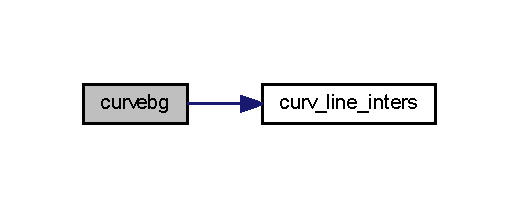
\includegraphics[width=249pt]{ellipgrid_8f90_adefdbbd93b3c42f5c88bf066fffda020_cgraph}
\end{center}
\end{figure}




Here is the caller graph for this function\+:
\nopagebreak
\begin{figure}[H]
\begin{center}
\leavevmode
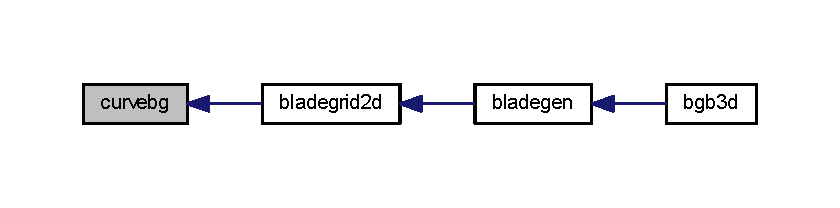
\includegraphics[width=350pt]{ellipgrid_8f90_adefdbbd93b3c42f5c88bf066fffda020_icgraph}
\end{center}
\end{figure}


\hypertarget{ellipgrid_8f90_acd54e32b03fd291e8ff39a8130d18f5c}{}\index{ellipgrid.\+f90@{ellipgrid.\+f90}!ellipdata@{ellipdata}}
\index{ellipdata@{ellipdata}!ellipgrid.\+f90@{ellipgrid.\+f90}}
\subsubsection[{ellipdata(xellip, yellip, xb, yb, np, uplmt)}]{\setlength{\rightskip}{0pt plus 5cm}subroutine ellipdata (
\begin{DoxyParamCaption}
\item[{real$\ast$8, dimension(np), intent(out)}]{xellip, }
\item[{real$\ast$8, dimension(np), intent(out)}]{yellip, }
\item[{real$\ast$8, dimension(np), intent(in)}]{xb, }
\item[{real$\ast$8, dimension(np), intent(in)}]{yb, }
\item[{integer}]{np, }
\item[{integer}]{uplmt}
\end{DoxyParamCaption}
)}\label{ellipgrid_8f90_acd54e32b03fd291e8ff39a8130d18f5c}


Here is the call graph for this function\+:
\nopagebreak
\begin{figure}[H]
\begin{center}
\leavevmode
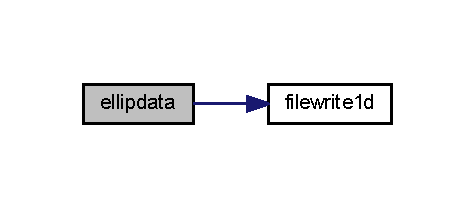
\includegraphics[width=228pt]{ellipgrid_8f90_acd54e32b03fd291e8ff39a8130d18f5c_cgraph}
\end{center}
\end{figure}


\hypertarget{ellipgrid_8f90_ac17e07f3b5ce7de5506c807ae6db88ef}{}\index{ellipgrid.\+f90@{ellipgrid.\+f90}!filewrite1d@{filewrite1d}}
\index{filewrite1d@{filewrite1d}!ellipgrid.\+f90@{ellipgrid.\+f90}}
\subsubsection[{filewrite1d(fname, X, Y, n)}]{\setlength{\rightskip}{0pt plus 5cm}subroutine filewrite1d (
\begin{DoxyParamCaption}
\item[{character$\ast$80, intent(in)}]{fname, }
\item[{real$\ast$8, dimension(n), intent(in)}]{X, }
\item[{real$\ast$8, dimension(n), intent(in)}]{Y, }
\item[{integer, intent(in)}]{n}
\end{DoxyParamCaption}
)}\label{ellipgrid_8f90_ac17e07f3b5ce7de5506c807ae6db88ef}


Here is the caller graph for this function\+:
\nopagebreak
\begin{figure}[H]
\begin{center}
\leavevmode
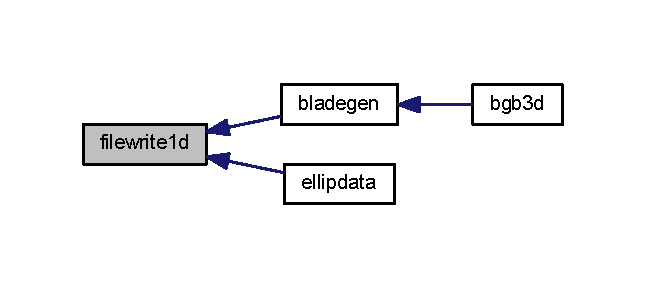
\includegraphics[width=310pt]{ellipgrid_8f90_ac17e07f3b5ce7de5506c807ae6db88ef_icgraph}
\end{center}
\end{figure}


\hypertarget{ellipgrid_8f90_a8c55d5a92c70a34a496062137ef35f6e}{}\index{ellipgrid.\+f90@{ellipgrid.\+f90}!filewritematrix@{filewritematrix}}
\index{filewritematrix@{filewritematrix}!ellipgrid.\+f90@{ellipgrid.\+f90}}
\subsubsection[{filewritematrix(fname, X, Y, nx, ny)}]{\setlength{\rightskip}{0pt plus 5cm}subroutine filewritematrix (
\begin{DoxyParamCaption}
\item[{character$\ast$32, intent(in)}]{fname, }
\item[{real$\ast$8, dimension(nx,ny), intent(in)}]{X, }
\item[{real$\ast$8, dimension(nx,ny), intent(in)}]{Y, }
\item[{integer, intent(in)}]{nx, }
\item[{integer, intent(in)}]{ny}
\end{DoxyParamCaption}
)}\label{ellipgrid_8f90_a8c55d5a92c70a34a496062137ef35f6e}


Here is the caller graph for this function\+:
\nopagebreak
\begin{figure}[H]
\begin{center}
\leavevmode
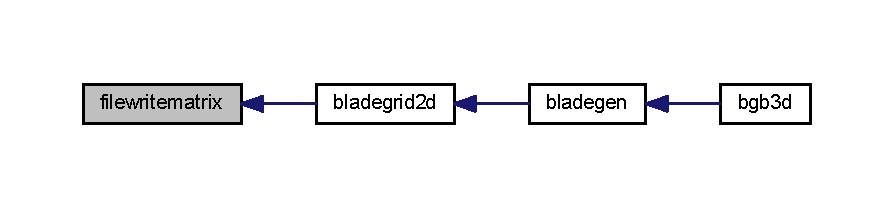
\includegraphics[width=350pt]{ellipgrid_8f90_a8c55d5a92c70a34a496062137ef35f6e_icgraph}
\end{center}
\end{figure}


\hypertarget{ellipgrid_8f90_ad37e0a5511289684f99d62342ff71a68}{}\index{ellipgrid.\+f90@{ellipgrid.\+f90}!gausei2d@{gausei2d}}
\index{gausei2d@{gausei2d}!ellipgrid.\+f90@{ellipgrid.\+f90}}
\subsubsection[{gausei2d(ni, nj, x, y, err, curvemesh, ellipsmooth)}]{\setlength{\rightskip}{0pt plus 5cm}subroutine gausei2d (
\begin{DoxyParamCaption}
\item[{integer}]{ni, }
\item[{integer}]{nj, }
\item[{real$\ast$8, dimension(ni,nj), intent(inout)}]{x, }
\item[{real$\ast$8, dimension(ni,nj), intent(inout)}]{y, }
\item[{real$\ast$8, intent(inout)}]{err, }
\item[{logical}]{curvemesh, }
\item[{logical}]{ellipsmooth}
\end{DoxyParamCaption}
)}\label{ellipgrid_8f90_ad37e0a5511289684f99d62342ff71a68}


Here is the caller graph for this function\+:
\nopagebreak
\begin{figure}[H]
\begin{center}
\leavevmode
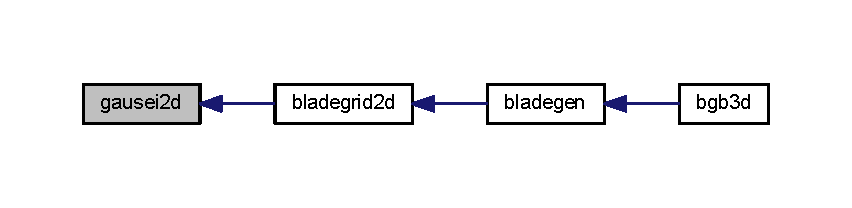
\includegraphics[width=350pt]{ellipgrid_8f90_ad37e0a5511289684f99d62342ff71a68_icgraph}
\end{center}
\end{figure}


\hypertarget{ellipgrid_8f90_a9700874d36140d2c7bee117590d5dae9}{}\index{ellipgrid.\+f90@{ellipgrid.\+f90}!gausei2dblade@{gausei2dblade}}
\index{gausei2dblade@{gausei2dblade}!ellipgrid.\+f90@{ellipgrid.\+f90}}
\subsubsection[{gausei2dblade(ni, nj, x, y, err, curvemesh, ellipsmooth, L\+E)}]{\setlength{\rightskip}{0pt plus 5cm}subroutine gausei2dblade (
\begin{DoxyParamCaption}
\item[{integer}]{ni, }
\item[{integer}]{nj, }
\item[{real$\ast$8, dimension(ni,nj), intent(inout)}]{x, }
\item[{real$\ast$8, dimension(ni,nj), intent(inout)}]{y, }
\item[{real$\ast$8, intent(inout)}]{err, }
\item[{logical}]{curvemesh, }
\item[{logical}]{ellipsmooth, }
\item[{integer}]{L\+E}
\end{DoxyParamCaption}
)}\label{ellipgrid_8f90_a9700874d36140d2c7bee117590d5dae9}


Here is the caller graph for this function\+:
\nopagebreak
\begin{figure}[H]
\begin{center}
\leavevmode
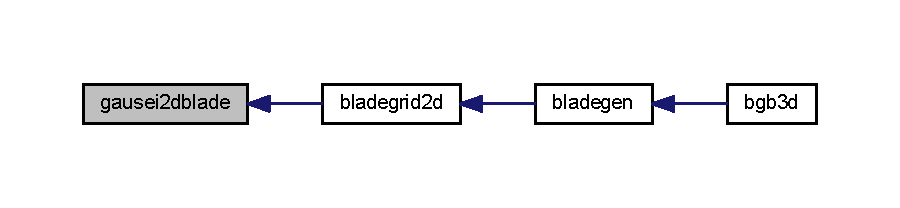
\includegraphics[width=350pt]{ellipgrid_8f90_a9700874d36140d2c7bee117590d5dae9_icgraph}
\end{center}
\end{figure}


\hypertarget{ellipgrid_8f90_a23f0130faf07695ae0633d37888c9298}{}\index{ellipgrid.\+f90@{ellipgrid.\+f90}!linearbg@{linearbg}}
\index{linearbg@{linearbg}!ellipgrid.\+f90@{ellipgrid.\+f90}}
\subsubsection[{linearbg(imax, jmax, xblade, yblade,                                               uplmt, np, casename, develop, msle, mble, chrd, pitch)}]{\setlength{\rightskip}{0pt plus 5cm}subroutine linearbg (
\begin{DoxyParamCaption}
\item[{integer, intent(out)}]{imax, }
\item[{integer, intent(out)}]{jmax, }
\item[{real$\ast$8, dimension(np), intent(in)}]{xblade, }
\item[{real$\ast$8, dimension(np), intent(in)}]{yblade, }
\item[{integer, intent(in)}]{uplmt, }
\item[{integer, intent(in)}]{np, }
\item[{character$\ast$32}]{casename, }
\item[{character$\ast$32}]{develop, }
\item[{real$\ast$8, intent(in)}]{msle, }
\item[{real$\ast$8, intent(in)}]{mble, }
\item[{real$\ast$8, intent(in)}]{chrd, }
\item[{real$\ast$8, intent(in)}]{pitch}
\end{DoxyParamCaption}
)}\label{ellipgrid_8f90_a23f0130faf07695ae0633d37888c9298}


Here is the caller graph for this function\+:
\nopagebreak
\begin{figure}[H]
\begin{center}
\leavevmode
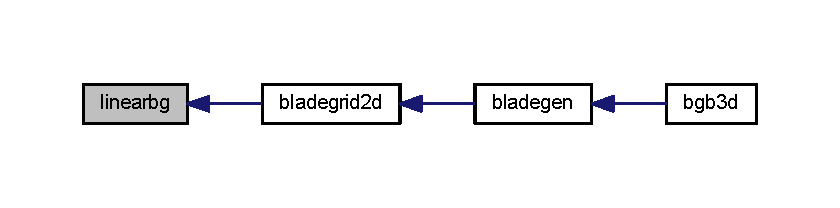
\includegraphics[width=350pt]{ellipgrid_8f90_a23f0130faf07695ae0633d37888c9298_icgraph}
\end{center}
\end{figure}


\hypertarget{ellipgrid_8f90_a341cb8880e0207c9fc41bc535fb8eb89}{}\index{ellipgrid.\+f90@{ellipgrid.\+f90}!offset\+\_\+points@{offset\+\_\+points}}
\index{offset\+\_\+points@{offset\+\_\+points}!ellipgrid.\+f90@{ellipgrid.\+f90}}
\subsubsection[{offset\+\_\+points(xnew, ynew, x, y, dxds, dyds, offset, npoints, k, uplmt, le\+\_\+pos, L\+E)}]{\setlength{\rightskip}{0pt plus 5cm}subroutine offset\+\_\+points (
\begin{DoxyParamCaption}
\item[{real$\ast$8, dimension(npoints)}]{xnew, }
\item[{real$\ast$8, dimension(npoints)}]{ynew, }
\item[{real$\ast$8, dimension(npoints)}]{x, }
\item[{real$\ast$8, dimension(npoints)}]{y, }
\item[{real$\ast$8, dimension(npoints)}]{dxds, }
\item[{real$\ast$8, dimension(npoints)}]{dyds, }
\item[{real$\ast$8}]{offset, }
\item[{integer}]{npoints, }
\item[{integer, intent(in)}]{k, }
\item[{integer, intent(in)}]{uplmt, }
\item[{integer, intent(in)}]{le\+\_\+pos, }
\item[{integer}]{L\+E}
\end{DoxyParamCaption}
)}\label{ellipgrid_8f90_a341cb8880e0207c9fc41bc535fb8eb89}


Here is the caller graph for this function\+:
\nopagebreak
\begin{figure}[H]
\begin{center}
\leavevmode
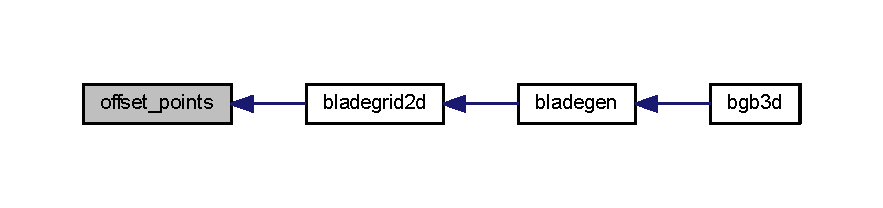
\includegraphics[width=350pt]{ellipgrid_8f90_a341cb8880e0207c9fc41bc535fb8eb89_icgraph}
\end{center}
\end{figure}


\hypertarget{ellipgrid_8f90_a812686a74c0d9667fd05b52300908671}{}\index{ellipgrid.\+f90@{ellipgrid.\+f90}!plot2d@{plot2d}}
\index{plot2d@{plot2d}!ellipgrid.\+f90@{ellipgrid.\+f90}}
\subsubsection[{plot2d(fname, x, y, nx, ny)}]{\setlength{\rightskip}{0pt plus 5cm}subroutine plot2d (
\begin{DoxyParamCaption}
\item[{character$\ast$32, intent(in)}]{fname, }
\item[{real$\ast$8, dimension(nx,ny), intent(in)}]{x, }
\item[{real$\ast$8, dimension(nx,ny), intent(in)}]{y, }
\item[{integer, intent(in)}]{nx, }
\item[{integer, intent(in)}]{ny}
\end{DoxyParamCaption}
)}\label{ellipgrid_8f90_a812686a74c0d9667fd05b52300908671}
\hypertarget{ellipgrid_8f90_ae47ef85c421748bee190d8cffa59a6cf}{}\index{ellipgrid.\+f90@{ellipgrid.\+f90}!stinglegrid@{stinglegrid}}
\index{stinglegrid@{stinglegrid}!ellipgrid.\+f90@{ellipgrid.\+f90}}
\subsubsection[{stinglegrid(xb, yb, np, uplmt, stingl, le\+\_\+pos, thkc, thick\+\_\+distr,                                                                                       mble, msle, mbte, chrd, jmax1, casename, fext, develop, isdev, etawidth)}]{\setlength{\rightskip}{0pt plus 5cm}subroutine stinglegrid (
\begin{DoxyParamCaption}
\item[{real$\ast$8, dimension(np), intent(in)}]{xb, }
\item[{real$\ast$8, dimension(np), intent(in)}]{yb, }
\item[{integer}]{np, }
\item[{integer}]{uplmt, }
\item[{real$\ast$8}]{stingl, }
\item[{integer}]{le\+\_\+pos, }
\item[{real$\ast$8}]{thkc, }
\item[{real$\ast$8}]{thick\+\_\+distr, }
\item[{real$\ast$8, intent(in)}]{mble, }
\item[{real$\ast$8, intent(in)}]{msle, }
\item[{real$\ast$8, intent(in)}]{mbte, }
\item[{real$\ast$8, intent(in)}]{chrd, }
\item[{integer}]{jmax1, }
\item[{character$\ast$32}]{casename, }
\item[{character$\ast$32}]{fext, }
\item[{character$\ast$32}]{develop, }
\item[{logical}]{isdev, }
\item[{real$\ast$8, intent(in)}]{etawidth}
\end{DoxyParamCaption}
)}\label{ellipgrid_8f90_ae47ef85c421748bee190d8cffa59a6cf}


Here is the call graph for this function\+:
\nopagebreak
\begin{figure}[H]
\begin{center}
\leavevmode
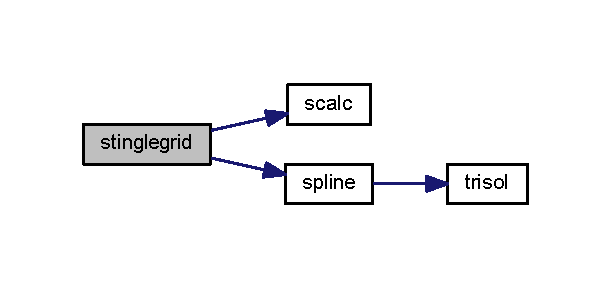
\includegraphics[width=293pt]{ellipgrid_8f90_ae47ef85c421748bee190d8cffa59a6cf_cgraph}
\end{center}
\end{figure}




Here is the caller graph for this function\+:
\nopagebreak
\begin{figure}[H]
\begin{center}
\leavevmode
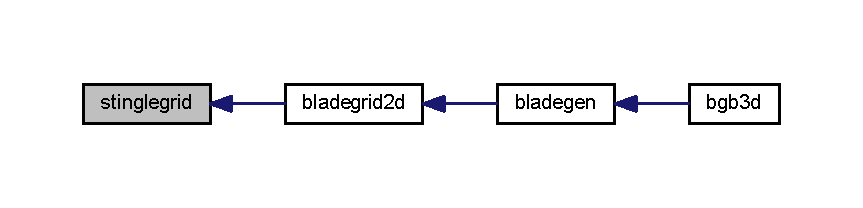
\includegraphics[width=350pt]{ellipgrid_8f90_ae47ef85c421748bee190d8cffa59a6cf_icgraph}
\end{center}
\end{figure}


\hypertarget{ellipgrid_8f90_aacf8b315a6f9a55076d90c6548dfe96c}{}\index{ellipgrid.\+f90@{ellipgrid.\+f90}!subdivide1d@{subdivide1d}}
\index{subdivide1d@{subdivide1d}!ellipgrid.\+f90@{ellipgrid.\+f90}}
\subsubsection[{subdivide1d(num1, num2, ratio)}]{\setlength{\rightskip}{0pt plus 5cm}real$\ast$8 function subdivide1d (
\begin{DoxyParamCaption}
\item[{real$\ast$8, dimension(1)}]{num1, }
\item[{real$\ast$8, dimension(1)}]{num2, }
\item[{real$\ast$8}]{ratio}
\end{DoxyParamCaption}
)}\label{ellipgrid_8f90_aacf8b315a6f9a55076d90c6548dfe96c}
\hypertarget{ellipgrid_8f90_a42a928bec1247db70e46f617b4d7e0d3}{}\index{ellipgrid.\+f90@{ellipgrid.\+f90}!subdivide2d@{subdivide2d}}
\index{subdivide2d@{subdivide2d}!ellipgrid.\+f90@{ellipgrid.\+f90}}
\subsubsection[{subdivide2d(num1, num2, ratio)}]{\setlength{\rightskip}{0pt plus 5cm}real$\ast$8 function subdivide2d (
\begin{DoxyParamCaption}
\item[{real$\ast$8, dimension(1,1)}]{num1, }
\item[{real$\ast$8, dimension(1,1)}]{num2, }
\item[{real$\ast$8}]{ratio}
\end{DoxyParamCaption}
)}\label{ellipgrid_8f90_a42a928bec1247db70e46f617b4d7e0d3}
\hypertarget{ellipgrid_8f90_a3f325469fb90d800dfdbcc323ffbd45d}{}\index{ellipgrid.\+f90@{ellipgrid.\+f90}!ycircle@{ycircle}}
\index{ycircle@{ycircle}!ellipgrid.\+f90@{ellipgrid.\+f90}}
\subsubsection[{ycircle(x, y, radius)}]{\setlength{\rightskip}{0pt plus 5cm}real$\ast$8 function ycircle (
\begin{DoxyParamCaption}
\item[{real$\ast$8, dimension(1), intent(in)}]{x, }
\item[{real$\ast$8, dimension(1), intent(in)}]{y, }
\item[{real$\ast$8, intent(in)}]{radius}
\end{DoxyParamCaption}
)}\label{ellipgrid_8f90_a3f325469fb90d800dfdbcc323ffbd45d}

\hypertarget{errors_8f90}{}\section{C\+:/\+Git3\+D\+B\+G\+B/source/errors.f90 File Reference}
\label{errors_8f90}\index{C\+:/\+Git3\+D\+B\+G\+B/source/errors.\+f90@{C\+:/\+Git3\+D\+B\+G\+B/source/errors.\+f90}}
\subsection*{Functions/\+Subroutines}
\begin{DoxyCompactItemize}
\item 
subroutine \hyperlink{errors_8f90_a8fe4eff2552c9e6fb855ac9c3b1567a1}{errors}
\end{DoxyCompactItemize}


\subsection{Function/\+Subroutine Documentation}
\hypertarget{errors_8f90_a8fe4eff2552c9e6fb855ac9c3b1567a1}{}\index{errors.\+f90@{errors.\+f90}!errors@{errors}}
\index{errors@{errors}!errors.\+f90@{errors.\+f90}}
\subsubsection[{errors}]{\setlength{\rightskip}{0pt plus 5cm}subroutine errors (
\begin{DoxyParamCaption}
{}
\end{DoxyParamCaption}
)}\label{errors_8f90_a8fe4eff2552c9e6fb855ac9c3b1567a1}

\hypertarget{func_nsubs_8f90}{}\section{C\+:/\+Git3\+D\+B\+G\+B/source/func\+Nsubs.f90 File Reference}
\label{func_nsubs_8f90}\index{C\+:/\+Git3\+D\+B\+G\+B/source/func\+Nsubs.\+f90@{C\+:/\+Git3\+D\+B\+G\+B/source/func\+Nsubs.\+f90}}
\subsection*{Functions/\+Subroutines}
\begin{DoxyCompactItemize}
\item 
subroutine \hyperlink{func_nsubs_8f90_a4a8bc1f698d94e09592f25a8bd194768}{displaymessage}
\item 
real $\ast$8 function \hyperlink{func_nsubs_8f90_a2ae2bc0834d61b30869f14490c600bf8}{inbetainci} (inbeta, inci)
\item 
real $\ast$8 function \hyperlink{func_nsubs_8f90_a56bc674499dfb930a1fcbdd96302b314}{outbetadevn} (inbeta, outbeta, devn)
\item 
subroutine \hyperlink{func_nsubs_8f90_ab0962397e03e040d57d95ffcd01c7647}{hubtipstreamline} (xhub, rhub, nphub, xtip, rtip, nptip, nsl, scf, casename)
\item 
subroutine \hyperlink{func_nsubs_8f90_af36676ddada4a392f839d5884a3f0994}{streamlines} (xml, rml, np, scf, casename, ia)
\item 
subroutine \hyperlink{func_nsubs_8f90_ac1c4ab8894f11e8e4a91c1caa86d6bde}{huboffset} (mphub, x, r, dxds, drds, hub, nphub, scf, casename)
\item 
subroutine \hyperlink{func_nsubs_8f90_a470359fa98c2e95400fba72c1ac5fcd5}{tipoffset} (mptip, x, r, dxds, drds, tip, nptip, scf, nsl, casename)
\item 
subroutine \hyperlink{func_nsubs_8f90_a93d13d26bea44378d2d6d3326ec1e4e3}{interp} (X\+A, Y\+A, X\+B, Y\+B, X\+C, Y\+C, X\+D, Y\+D, X\+I\+N\+T, Y\+I\+N\+T)
\item 
subroutine \hyperlink{func_nsubs_8f90_ac18c0448926e39757d71d4a34252e5b8}{outputfiledata} (bladedata, nsl, amount\+\_\+data, throat\+\_\+pos, casename, units)
\item 
subroutine \hyperlink{func_nsubs_8f90_a704ccaa1ae9d68875970c62c51a4880e}{throatindex} (throat\+\_\+pos, throat\+\_\+index, n\+\_\+normal\+\_\+distance, js, nsl)
\item 
subroutine \hyperlink{func_nsubs_8f90_ae04f7bd8c70f97d1b0497a335b6d278c}{cascade\+\_\+nondim\+\_\+file} (msle, mste, mprime\+\_\+ble, mprime\+\_\+bte, chordm, pitch, nsl, ibrow, casename)
\item 
subroutine \hyperlink{func_nsubs_8f90_a788e8b317e0de3c84602920daaade52b}{aecalc} (n, x, y, t, itype, area, xcen, ycen, ei11, ei22, apx1, apx2)
\item 
subroutine \hyperlink{func_nsubs_8f90_ac45892d1114b6596d21635c8ff1c9429}{stacking} (xb, yb, xbot, ybot, xtop, ytop, js, np, stack\+\_\+switch, stack, stk\+\_\+u, stk\+\_\+v, area, L\+E)
\item 
subroutine \hyperlink{func_nsubs_8f90_a769176856aeaec2c9518c91f01f5f4fe}{rotate} (xb, yb, x, y, \hyperlink{bsplinecam_8f90_af4379365bf9e92538191fcb377a6e7fa}{angle})
\item 
subroutine \hyperlink{func_nsubs_8f90_a94eb8a9dd035c46326a5720675b5eca7}{rotate2} (xb, yb, x, y, \hyperlink{bsplinecam_8f90_af4379365bf9e92538191fcb377a6e7fa}{angle})
\item 
real function \hyperlink{func_nsubs_8f90_a50bc8afe7f9e452ccb73514e97ca797a}{scaled} (x, scalefactor)
\item 
subroutine \hyperlink{func_nsubs_8f90_a91a04c46162d2923e385fb150c9dd7c7}{bladesection} (xb, yb, np, nbls, T\+E\+\_\+del, sinls, sexts, chrdd, fext, js, pitch, mble, mbte, airfoil)
\item 
subroutine \hyperlink{func_nsubs_8f90_ae926fe9b2bcad043feaf1b7e5f4e7ab6}{st\+\_\+line\+\_\+intersection} (X\+A, Y\+A, X\+B, Y\+B, X\+C, Y\+C, X\+D, Y\+D, X\+I\+N\+T, Y\+I\+N\+T)
\item 
subroutine \hyperlink{func_nsubs_8f90_ad23786e7bb8cf9c0b066f4bc0930a172}{throat\+\_\+calc\+\_\+pitch\+\_\+line} (xb, yb, np, \hyperlink{bsplinecam_8f90_a5f344dd1ac7aa0679039a2bd0531aec6}{camber}, \hyperlink{bsplinecam_8f90_af4379365bf9e92538191fcb377a6e7fa}{angle}, sang, u, pi, pitch, throat\+\_\+coord, mouth\+\_\+coord, exit\+\_\+coord,                                                                                                                                   min\+\_\+throat\+\_\+2\+D, throat\+\_\+index, n\+\_\+normal\+\_\+distance, casename, js, nsl, develop, isdev)
\item 
subroutine \hyperlink{func_nsubs_8f90_ada1a18ee307fefd9aad27217363e594f}{averaged\+\_\+camber} (xb, yb, np, u, \hyperlink{bsplinecam_8f90_a5f344dd1ac7aa0679039a2bd0531aec6}{camber}, \hyperlink{bsplinecam_8f90_af4379365bf9e92538191fcb377a6e7fa}{angle}, sinl)
\item 
subroutine \hyperlink{func_nsubs_8f90_ada44c10e93da7731616a3c34a28951e3}{askr} (prompt, rinput)
\item 
subroutine \hyperlink{func_nsubs_8f90_ac9fbd4cb2aee0e492314a37b00788ff1}{meanline3dnperiodicwall} (xb, yb, zb, xposlean, yposlean, zposlean,                                                                                                                                       xneglean, yneglean, zneglean, iap, nsec,                                                                                                                                       uplmt, scf, casename)
\item 
real $\ast$8 function \hyperlink{func_nsubs_8f90_adedcaf9d0c76801d354dbe2ab22f9f83}{numoffset} (num, delta)
\item 
subroutine \hyperlink{func_nsubs_8f90_a0e9c807d58ef2f7306cf94646c7f307d}{constantslopemeanline3d} (xb, yb, zb, xposlean, yposlean, zposlean,                                                                                                                                       xneglean, yneglean, zneglean, iap, nsec,                                                                                                                                       uplmt, scf, casename)
\end{DoxyCompactItemize}


\subsection{Function/\+Subroutine Documentation}
\hypertarget{func_nsubs_8f90_a788e8b317e0de3c84602920daaade52b}{}\index{func\+Nsubs.\+f90@{func\+Nsubs.\+f90}!aecalc@{aecalc}}
\index{aecalc@{aecalc}!func\+Nsubs.\+f90@{func\+Nsubs.\+f90}}
\subsubsection[{aecalc(n, x, y, t, itype, area, xcen, ycen, ei11, ei22, apx1, apx2)}]{\setlength{\rightskip}{0pt plus 5cm}subroutine aecalc (
\begin{DoxyParamCaption}
\item[{}]{n, }
\item[{dimension(n)}]{x, }
\item[{dimension(n)}]{y, }
\item[{dimension(n)}]{t, }
\item[{}]{itype, }
\item[{}]{area, }
\item[{}]{xcen, }
\item[{}]{ycen, }
\item[{}]{ei11, }
\item[{}]{ei22, }
\item[{}]{apx1, }
\item[{}]{apx2}
\end{DoxyParamCaption}
)}\label{func_nsubs_8f90_a788e8b317e0de3c84602920daaade52b}


Here is the caller graph for this function\+:
\nopagebreak
\begin{figure}[H]
\begin{center}
\leavevmode
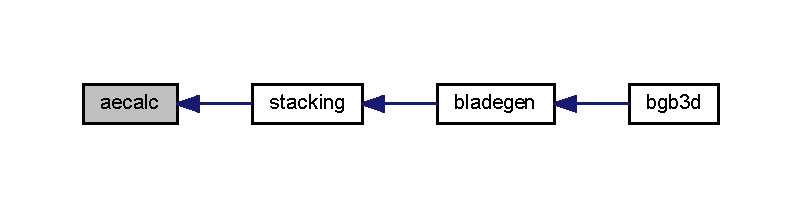
\includegraphics[width=350pt]{func_nsubs_8f90_a788e8b317e0de3c84602920daaade52b_icgraph}
\end{center}
\end{figure}


\hypertarget{func_nsubs_8f90_ada44c10e93da7731616a3c34a28951e3}{}\index{func\+Nsubs.\+f90@{func\+Nsubs.\+f90}!askr@{askr}}
\index{askr@{askr}!func\+Nsubs.\+f90@{func\+Nsubs.\+f90}}
\subsubsection[{askr(prompt, rinput)}]{\setlength{\rightskip}{0pt plus 5cm}subroutine askr (
\begin{DoxyParamCaption}
\item[{character$\ast$($\ast$)}]{prompt, }
\item[{real}]{rinput}
\end{DoxyParamCaption}
)}\label{func_nsubs_8f90_ada44c10e93da7731616a3c34a28951e3}
\hypertarget{func_nsubs_8f90_ada1a18ee307fefd9aad27217363e594f}{}\index{func\+Nsubs.\+f90@{func\+Nsubs.\+f90}!averaged\+\_\+camber@{averaged\+\_\+camber}}
\index{averaged\+\_\+camber@{averaged\+\_\+camber}!func\+Nsubs.\+f90@{func\+Nsubs.\+f90}}
\subsubsection[{averaged\+\_\+camber(xb, yb, np, u, camber, angle, sinl)}]{\setlength{\rightskip}{0pt plus 5cm}subroutine averaged\+\_\+camber (
\begin{DoxyParamCaption}
\item[{real, dimension(np)}]{xb, }
\item[{real, dimension(np)}]{yb, }
\item[{integer}]{np, }
\item[{real, dimension((np+1)/2)}]{u, }
\item[{real, dimension((np+1)/2)}]{camber, }
\item[{real, dimension((np+1)/2)}]{angle, }
\item[{real}]{sinl}
\end{DoxyParamCaption}
)}\label{func_nsubs_8f90_ada1a18ee307fefd9aad27217363e594f}


Here is the caller graph for this function\+:
\nopagebreak
\begin{figure}[H]
\begin{center}
\leavevmode
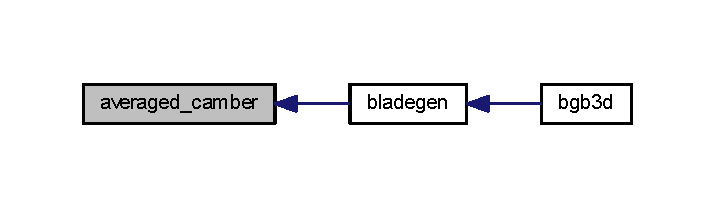
\includegraphics[width=343pt]{func_nsubs_8f90_ada1a18ee307fefd9aad27217363e594f_icgraph}
\end{center}
\end{figure}


\hypertarget{func_nsubs_8f90_a91a04c46162d2923e385fb150c9dd7c7}{}\index{func\+Nsubs.\+f90@{func\+Nsubs.\+f90}!bladesection@{bladesection}}
\index{bladesection@{bladesection}!func\+Nsubs.\+f90@{func\+Nsubs.\+f90}}
\subsubsection[{bladesection(xb, yb, np, nbls, T\+E\+\_\+del, sinls, sexts, chrdd, fext, js, pitch, mble, mbte, airfoil)}]{\setlength{\rightskip}{0pt plus 5cm}subroutine bladesection (
\begin{DoxyParamCaption}
\item[{real$\ast$8, dimension(nx), intent(inout)}]{xb, }
\item[{real$\ast$8, dimension(nx), intent(inout)}]{yb, }
\item[{integer}]{np, }
\item[{integer}]{nbls, }
\item[{integer}]{T\+E\+\_\+del, }
\item[{real$\ast$8}]{sinls, }
\item[{real$\ast$8}]{sexts, }
\item[{real$\ast$8}]{chrdd, }
\item[{character$\ast$32}]{fext, }
\item[{integer}]{js, }
\item[{real$\ast$8}]{pitch, }
\item[{real$\ast$8}]{mble, }
\item[{real$\ast$8}]{mbte, }
\item[{character$\ast$20}]{airfoil}
\end{DoxyParamCaption}
)}\label{func_nsubs_8f90_a91a04c46162d2923e385fb150c9dd7c7}


Here is the caller graph for this function\+:
\nopagebreak
\begin{figure}[H]
\begin{center}
\leavevmode
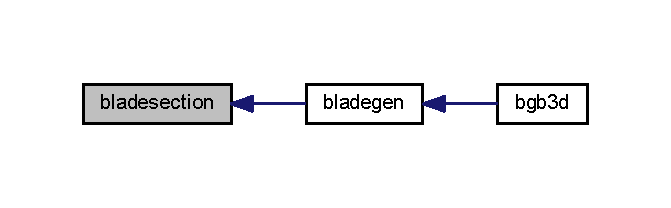
\includegraphics[width=322pt]{func_nsubs_8f90_a91a04c46162d2923e385fb150c9dd7c7_icgraph}
\end{center}
\end{figure}


\hypertarget{func_nsubs_8f90_ae04f7bd8c70f97d1b0497a335b6d278c}{}\index{func\+Nsubs.\+f90@{func\+Nsubs.\+f90}!cascade\+\_\+nondim\+\_\+file@{cascade\+\_\+nondim\+\_\+file}}
\index{cascade\+\_\+nondim\+\_\+file@{cascade\+\_\+nondim\+\_\+file}!func\+Nsubs.\+f90@{func\+Nsubs.\+f90}}
\subsubsection[{cascade\+\_\+nondim\+\_\+file(msle, mste, mprime\+\_\+ble, mprime\+\_\+bte, chordm, pitch, nsl, ibrow, casename)}]{\setlength{\rightskip}{0pt plus 5cm}subroutine cascade\+\_\+nondim\+\_\+file (
\begin{DoxyParamCaption}
\item[{real$\ast$8, dimension(nsl), intent(in)}]{msle, }
\item[{real$\ast$8, dimension(nsl), intent(in)}]{mste, }
\item[{real$\ast$8, dimension(nsl), intent(in)}]{mprime\+\_\+ble, }
\item[{real$\ast$8, dimension(nsl), intent(in)}]{mprime\+\_\+bte, }
\item[{real$\ast$8, dimension(nsl), intent(in)}]{chordm, }
\item[{real$\ast$8, intent(in)}]{pitch, }
\item[{integer, intent(in)}]{nsl, }
\item[{integer, intent(in)}]{ibrow, }
\item[{character$\ast$32}]{casename}
\end{DoxyParamCaption}
)}\label{func_nsubs_8f90_ae04f7bd8c70f97d1b0497a335b6d278c}


Here is the caller graph for this function\+:
\nopagebreak
\begin{figure}[H]
\begin{center}
\leavevmode
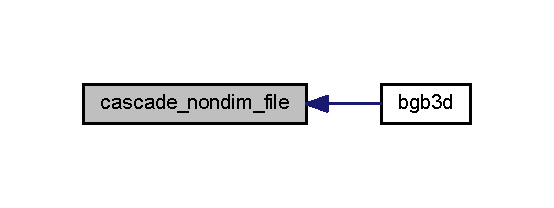
\includegraphics[width=266pt]{func_nsubs_8f90_ae04f7bd8c70f97d1b0497a335b6d278c_icgraph}
\end{center}
\end{figure}


\hypertarget{func_nsubs_8f90_a0e9c807d58ef2f7306cf94646c7f307d}{}\index{func\+Nsubs.\+f90@{func\+Nsubs.\+f90}!constantslopemeanline3d@{constantslopemeanline3d}}
\index{constantslopemeanline3d@{constantslopemeanline3d}!func\+Nsubs.\+f90@{func\+Nsubs.\+f90}}
\subsubsection[{constantslopemeanline3d(xb, yb, zb, xposlean, yposlean, zposlean,                                                                                                                                       xneglean, yneglean, zneglean, iap, nsec,                                                                                                                                       uplmt, scf, casename)}]{\setlength{\rightskip}{0pt plus 5cm}subroutine constantslopemeanline3d (
\begin{DoxyParamCaption}
\item[{real$\ast$8, dimension(iap,nsec), intent(in)}]{xb, }
\item[{real$\ast$8, dimension(iap,nsec), intent(in)}]{yb, }
\item[{real$\ast$8, dimension(iap,nsec), intent(in)}]{zb, }
\item[{real$\ast$8, dimension(iap,nsec), intent(in)}]{xposlean, }
\item[{real$\ast$8, dimension(iap,nsec), intent(in)}]{yposlean, }
\item[{real$\ast$8, dimension(iap,nsec), intent(in)}]{zposlean, }
\item[{real$\ast$8, dimension(iap,nsec), intent(in)}]{xneglean, }
\item[{real$\ast$8, dimension(iap,nsec), intent(in)}]{yneglean, }
\item[{real$\ast$8, dimension(iap,nsec), intent(in)}]{zneglean, }
\item[{integer, intent(in)}]{iap, }
\item[{integer, intent(in)}]{nsec, }
\item[{integer, intent(in)}]{uplmt, }
\item[{real$\ast$8, intent(in)}]{scf, }
\item[{character$\ast$32}]{casename}
\end{DoxyParamCaption}
)}\label{func_nsubs_8f90_a0e9c807d58ef2f7306cf94646c7f307d}


Here is the caller graph for this function\+:
\nopagebreak
\begin{figure}[H]
\begin{center}
\leavevmode
\includegraphics[width=350pt]{func_nsubs_8f90_a0e9c807d58ef2f7306cf94646c7f307d_icgraph}
\end{center}
\end{figure}


\hypertarget{func_nsubs_8f90_a4a8bc1f698d94e09592f25a8bd194768}{}\index{func\+Nsubs.\+f90@{func\+Nsubs.\+f90}!displaymessage@{displaymessage}}
\index{displaymessage@{displaymessage}!func\+Nsubs.\+f90@{func\+Nsubs.\+f90}}
\subsubsection[{displaymessage}]{\setlength{\rightskip}{0pt plus 5cm}subroutine displaymessage (
\begin{DoxyParamCaption}
{}
\end{DoxyParamCaption}
)}\label{func_nsubs_8f90_a4a8bc1f698d94e09592f25a8bd194768}


Here is the caller graph for this function\+:
\nopagebreak
\begin{figure}[H]
\begin{center}
\leavevmode
\includegraphics[width=246pt]{func_nsubs_8f90_a4a8bc1f698d94e09592f25a8bd194768_icgraph}
\end{center}
\end{figure}


\hypertarget{func_nsubs_8f90_ac1c4ab8894f11e8e4a91c1caa86d6bde}{}\index{func\+Nsubs.\+f90@{func\+Nsubs.\+f90}!huboffset@{huboffset}}
\index{huboffset@{huboffset}!func\+Nsubs.\+f90@{func\+Nsubs.\+f90}}
\subsubsection[{huboffset(mphub, x, r, dxds, drds, hub, nphub, scf, casename)}]{\setlength{\rightskip}{0pt plus 5cm}subroutine huboffset (
\begin{DoxyParamCaption}
\item[{real$\ast$8, dimension(nphub,1), intent(out)}]{mphub, }
\item[{real$\ast$8, dimension(nphub,1)}]{x, }
\item[{real$\ast$8, dimension(nphub,1)}]{r, }
\item[{real$\ast$8, dimension(nphub,1)}]{dxds, }
\item[{real$\ast$8, dimension(nphub,1)}]{drds, }
\item[{real$\ast$8}]{hub, }
\item[{integer}]{nphub, }
\item[{real$\ast$8}]{scf, }
\item[{character$\ast$32}]{casename}
\end{DoxyParamCaption}
)}\label{func_nsubs_8f90_ac1c4ab8894f11e8e4a91c1caa86d6bde}


Here is the call graph for this function\+:
\nopagebreak
\begin{figure}[H]
\begin{center}
\leavevmode
\includegraphics[width=288pt]{func_nsubs_8f90_ac1c4ab8894f11e8e4a91c1caa86d6bde_cgraph}
\end{center}
\end{figure}




Here is the caller graph for this function\+:
\nopagebreak
\begin{figure}[H]
\begin{center}
\leavevmode
\includegraphics[width=215pt]{func_nsubs_8f90_ac1c4ab8894f11e8e4a91c1caa86d6bde_icgraph}
\end{center}
\end{figure}


\hypertarget{func_nsubs_8f90_ab0962397e03e040d57d95ffcd01c7647}{}\index{func\+Nsubs.\+f90@{func\+Nsubs.\+f90}!hubtipstreamline@{hubtipstreamline}}
\index{hubtipstreamline@{hubtipstreamline}!func\+Nsubs.\+f90@{func\+Nsubs.\+f90}}
\subsubsection[{hubtipstreamline(xhub, rhub, nphub, xtip, rtip, nptip, nsl, scf, casename)}]{\setlength{\rightskip}{0pt plus 5cm}subroutine hubtipstreamline (
\begin{DoxyParamCaption}
\item[{real$\ast$8, dimension(nphub,1)}]{xhub, }
\item[{real$\ast$8, dimension(nphub,1)}]{rhub, }
\item[{integer}]{nphub, }
\item[{real$\ast$8, dimension(nptip,1)}]{xtip, }
\item[{real$\ast$8, dimension(nptip,1)}]{rtip, }
\item[{integer}]{nptip, }
\item[{integer}]{nsl, }
\item[{real$\ast$8}]{scf, }
\item[{character$\ast$32}]{casename}
\end{DoxyParamCaption}
)}\label{func_nsubs_8f90_ab0962397e03e040d57d95ffcd01c7647}


Here is the caller graph for this function\+:
\nopagebreak
\begin{figure}[H]
\begin{center}
\leavevmode
\includegraphics[width=247pt]{func_nsubs_8f90_ab0962397e03e040d57d95ffcd01c7647_icgraph}
\end{center}
\end{figure}


\hypertarget{func_nsubs_8f90_a2ae2bc0834d61b30869f14490c600bf8}{}\index{func\+Nsubs.\+f90@{func\+Nsubs.\+f90}!inbetainci@{inbetainci}}
\index{inbetainci@{inbetainci}!func\+Nsubs.\+f90@{func\+Nsubs.\+f90}}
\subsubsection[{inbetainci(inbeta, inci)}]{\setlength{\rightskip}{0pt plus 5cm}real$\ast$8 function inbetainci (
\begin{DoxyParamCaption}
\item[{real$\ast$8, dimension(1)}]{inbeta, }
\item[{real$\ast$8, dimension(1)}]{inci}
\end{DoxyParamCaption}
)}\label{func_nsubs_8f90_a2ae2bc0834d61b30869f14490c600bf8}
\hypertarget{func_nsubs_8f90_a93d13d26bea44378d2d6d3326ec1e4e3}{}\index{func\+Nsubs.\+f90@{func\+Nsubs.\+f90}!interp@{interp}}
\index{interp@{interp}!func\+Nsubs.\+f90@{func\+Nsubs.\+f90}}
\subsubsection[{interp(\+X\+A, Y\+A, X\+B, Y\+B, X\+C, Y\+C, X\+D, Y\+D, X\+I\+N\+T, Y\+I\+N\+T)}]{\setlength{\rightskip}{0pt plus 5cm}subroutine interp (
\begin{DoxyParamCaption}
\item[{real$\ast$8}]{X\+A, }
\item[{real$\ast$8}]{Y\+A, }
\item[{real$\ast$8}]{X\+B, }
\item[{real$\ast$8}]{Y\+B, }
\item[{real$\ast$8}]{X\+C, }
\item[{real$\ast$8}]{Y\+C, }
\item[{real$\ast$8}]{X\+D, }
\item[{real$\ast$8}]{Y\+D, }
\item[{real$\ast$8}]{X\+I\+N\+T, }
\item[{real$\ast$8}]{Y\+I\+N\+T}
\end{DoxyParamCaption}
)}\label{func_nsubs_8f90_a93d13d26bea44378d2d6d3326ec1e4e3}
\hypertarget{func_nsubs_8f90_ac9fbd4cb2aee0e492314a37b00788ff1}{}\index{func\+Nsubs.\+f90@{func\+Nsubs.\+f90}!meanline3dnperiodicwall@{meanline3dnperiodicwall}}
\index{meanline3dnperiodicwall@{meanline3dnperiodicwall}!func\+Nsubs.\+f90@{func\+Nsubs.\+f90}}
\subsubsection[{meanline3dnperiodicwall(xb, yb, zb, xposlean, yposlean, zposlean,                                                                                                                                       xneglean, yneglean, zneglean, iap, nsec,                                                                                                                                       uplmt, scf, casename)}]{\setlength{\rightskip}{0pt plus 5cm}subroutine meanline3dnperiodicwall (
\begin{DoxyParamCaption}
\item[{real$\ast$8, dimension(iap,nsec), intent(in)}]{xb, }
\item[{real$\ast$8, dimension(iap,nsec), intent(in)}]{yb, }
\item[{real$\ast$8, dimension(iap,nsec), intent(in)}]{zb, }
\item[{real$\ast$8, dimension(iap,nsec), intent(in)}]{xposlean, }
\item[{real$\ast$8, dimension(iap,nsec), intent(in)}]{yposlean, }
\item[{real$\ast$8, dimension(iap,nsec), intent(in)}]{zposlean, }
\item[{real$\ast$8, dimension(iap,nsec), intent(in)}]{xneglean, }
\item[{real$\ast$8, dimension(iap,nsec), intent(in)}]{yneglean, }
\item[{real$\ast$8, dimension(iap,nsec), intent(in)}]{zneglean, }
\item[{integer, intent(in)}]{iap, }
\item[{integer, intent(in)}]{nsec, }
\item[{integer, intent(in)}]{uplmt, }
\item[{real$\ast$8, intent(in)}]{scf, }
\item[{character$\ast$32}]{casename}
\end{DoxyParamCaption}
)}\label{func_nsubs_8f90_ac9fbd4cb2aee0e492314a37b00788ff1}
\hypertarget{func_nsubs_8f90_adedcaf9d0c76801d354dbe2ab22f9f83}{}\index{func\+Nsubs.\+f90@{func\+Nsubs.\+f90}!numoffset@{numoffset}}
\index{numoffset@{numoffset}!func\+Nsubs.\+f90@{func\+Nsubs.\+f90}}
\subsubsection[{numoffset(num, delta)}]{\setlength{\rightskip}{0pt plus 5cm}real$\ast$8 function numoffset (
\begin{DoxyParamCaption}
\item[{real$\ast$8, dimension(1)}]{num, }
\item[{real$\ast$8}]{delta}
\end{DoxyParamCaption}
)}\label{func_nsubs_8f90_adedcaf9d0c76801d354dbe2ab22f9f83}
\hypertarget{func_nsubs_8f90_a56bc674499dfb930a1fcbdd96302b314}{}\index{func\+Nsubs.\+f90@{func\+Nsubs.\+f90}!outbetadevn@{outbetadevn}}
\index{outbetadevn@{outbetadevn}!func\+Nsubs.\+f90@{func\+Nsubs.\+f90}}
\subsubsection[{outbetadevn(inbeta, outbeta, devn)}]{\setlength{\rightskip}{0pt plus 5cm}real$\ast$8 function outbetadevn (
\begin{DoxyParamCaption}
\item[{real$\ast$8, dimension(1)}]{inbeta, }
\item[{real$\ast$8, dimension(1)}]{outbeta, }
\item[{real$\ast$8, dimension(1)}]{devn}
\end{DoxyParamCaption}
)}\label{func_nsubs_8f90_a56bc674499dfb930a1fcbdd96302b314}
\hypertarget{func_nsubs_8f90_ac18c0448926e39757d71d4a34252e5b8}{}\index{func\+Nsubs.\+f90@{func\+Nsubs.\+f90}!outputfiledata@{outputfiledata}}
\index{outputfiledata@{outputfiledata}!func\+Nsubs.\+f90@{func\+Nsubs.\+f90}}
\subsubsection[{outputfiledata(bladedata, nsl, amount\+\_\+data, throat\+\_\+pos, casename, units)}]{\setlength{\rightskip}{0pt plus 5cm}subroutine outputfiledata (
\begin{DoxyParamCaption}
\item[{real$\ast$4, dimension(amount\+\_\+data,nsl)}]{bladedata, }
\item[{integer}]{nsl, }
\item[{integer}]{amount\+\_\+data, }
\item[{character$\ast$20, dimension(nsl)}]{throat\+\_\+pos, }
\item[{character$\ast$32}]{casename, }
\item[{character(len=2)}]{units}
\end{DoxyParamCaption}
)}\label{func_nsubs_8f90_ac18c0448926e39757d71d4a34252e5b8}


Here is the caller graph for this function\+:
\nopagebreak
\begin{figure}[H]
\begin{center}
\leavevmode
\includegraphics[width=233pt]{func_nsubs_8f90_ac18c0448926e39757d71d4a34252e5b8_icgraph}
\end{center}
\end{figure}


\hypertarget{func_nsubs_8f90_a769176856aeaec2c9518c91f01f5f4fe}{}\index{func\+Nsubs.\+f90@{func\+Nsubs.\+f90}!rotate@{rotate}}
\index{rotate@{rotate}!func\+Nsubs.\+f90@{func\+Nsubs.\+f90}}
\subsubsection[{rotate(xb, yb, x, y, angle)}]{\setlength{\rightskip}{0pt plus 5cm}subroutine rotate (
\begin{DoxyParamCaption}
\item[{real, dimension(1), intent(out)}]{xb, }
\item[{real, dimension(1), intent(out)}]{yb, }
\item[{real}]{x, }
\item[{real}]{y, }
\item[{real}]{angle}
\end{DoxyParamCaption}
)}\label{func_nsubs_8f90_a769176856aeaec2c9518c91f01f5f4fe}


Here is the caller graph for this function\+:
\nopagebreak
\begin{figure}[H]
\begin{center}
\leavevmode
\includegraphics[width=292pt]{func_nsubs_8f90_a769176856aeaec2c9518c91f01f5f4fe_icgraph}
\end{center}
\end{figure}


\hypertarget{func_nsubs_8f90_a94eb8a9dd035c46326a5720675b5eca7}{}\index{func\+Nsubs.\+f90@{func\+Nsubs.\+f90}!rotate2@{rotate2}}
\index{rotate2@{rotate2}!func\+Nsubs.\+f90@{func\+Nsubs.\+f90}}
\subsubsection[{rotate2(xb, yb, x, y, angle)}]{\setlength{\rightskip}{0pt plus 5cm}subroutine rotate2 (
\begin{DoxyParamCaption}
\item[{real, intent(out)}]{xb, }
\item[{real, intent(out)}]{yb, }
\item[{real}]{x, }
\item[{real}]{y, }
\item[{real}]{angle}
\end{DoxyParamCaption}
)}\label{func_nsubs_8f90_a94eb8a9dd035c46326a5720675b5eca7}


Here is the caller graph for this function\+:
\nopagebreak
\begin{figure}[H]
\begin{center}
\leavevmode
\includegraphics[width=298pt]{func_nsubs_8f90_a94eb8a9dd035c46326a5720675b5eca7_icgraph}
\end{center}
\end{figure}


\hypertarget{func_nsubs_8f90_a50bc8afe7f9e452ccb73514e97ca797a}{}\index{func\+Nsubs.\+f90@{func\+Nsubs.\+f90}!scaled@{scaled}}
\index{scaled@{scaled}!func\+Nsubs.\+f90@{func\+Nsubs.\+f90}}
\subsubsection[{scaled(x, scalefactor)}]{\setlength{\rightskip}{0pt plus 5cm}real function scaled (
\begin{DoxyParamCaption}
\item[{real, intent(in)}]{x, }
\item[{real, intent(in)}]{scalefactor}
\end{DoxyParamCaption}
)}\label{func_nsubs_8f90_a50bc8afe7f9e452ccb73514e97ca797a}
\hypertarget{func_nsubs_8f90_ae926fe9b2bcad043feaf1b7e5f4e7ab6}{}\index{func\+Nsubs.\+f90@{func\+Nsubs.\+f90}!st\+\_\+line\+\_\+intersection@{st\+\_\+line\+\_\+intersection}}
\index{st\+\_\+line\+\_\+intersection@{st\+\_\+line\+\_\+intersection}!func\+Nsubs.\+f90@{func\+Nsubs.\+f90}}
\subsubsection[{st\+\_\+line\+\_\+intersection(\+X\+A, Y\+A, X\+B, Y\+B, X\+C, Y\+C, X\+D, Y\+D, X\+I\+N\+T, Y\+I\+N\+T)}]{\setlength{\rightskip}{0pt plus 5cm}subroutine st\+\_\+line\+\_\+intersection (
\begin{DoxyParamCaption}
\item[{real$\ast$8}]{X\+A, }
\item[{real$\ast$8}]{Y\+A, }
\item[{real$\ast$8}]{X\+B, }
\item[{real$\ast$8}]{Y\+B, }
\item[{real$\ast$8}]{X\+C, }
\item[{real$\ast$8}]{Y\+C, }
\item[{real$\ast$8}]{X\+D, }
\item[{real$\ast$8}]{Y\+D, }
\item[{real$\ast$8, intent(out)}]{X\+I\+N\+T, }
\item[{real$\ast$8, intent(out)}]{Y\+I\+N\+T}
\end{DoxyParamCaption}
)}\label{func_nsubs_8f90_ae926fe9b2bcad043feaf1b7e5f4e7ab6}


Here is the caller graph for this function\+:
\nopagebreak
\begin{figure}[H]
\begin{center}
\leavevmode
\includegraphics[width=350pt]{func_nsubs_8f90_ae926fe9b2bcad043feaf1b7e5f4e7ab6_icgraph}
\end{center}
\end{figure}


\hypertarget{func_nsubs_8f90_ac45892d1114b6596d21635c8ff1c9429}{}\index{func\+Nsubs.\+f90@{func\+Nsubs.\+f90}!stacking@{stacking}}
\index{stacking@{stacking}!func\+Nsubs.\+f90@{func\+Nsubs.\+f90}}
\subsubsection[{stacking(xb, yb, xbot, ybot, xtop, ytop, js, np, stack\+\_\+switch, stack, stk\+\_\+u, stk\+\_\+v, area, L\+E)}]{\setlength{\rightskip}{0pt plus 5cm}subroutine stacking (
\begin{DoxyParamCaption}
\item[{real, dimension(np), intent(inout)}]{xb, }
\item[{real, dimension(np), intent(inout)}]{yb, }
\item[{real, dimension((np+1)/2), intent(inout)}]{xbot, }
\item[{real, dimension((np+1)/2), intent(inout)}]{ybot, }
\item[{real, dimension((np+1)/2), intent(inout)}]{xtop, }
\item[{real, dimension((np+1)/2), intent(inout)}]{ytop, }
\item[{integer, intent(in)}]{js, }
\item[{integer}]{np, }
\item[{integer, intent(in)}]{stack\+\_\+switch, }
\item[{integer, intent(in)}]{stack, }
\item[{real, dimension(1), intent(in)}]{stk\+\_\+u, }
\item[{real, dimension(1), intent(in)}]{stk\+\_\+v, }
\item[{real}]{area, }
\item[{integer}]{L\+E}
\end{DoxyParamCaption}
)}\label{func_nsubs_8f90_ac45892d1114b6596d21635c8ff1c9429}


Here is the call graph for this function\+:
\nopagebreak
\begin{figure}[H]
\begin{center}
\leavevmode
\includegraphics[width=214pt]{func_nsubs_8f90_ac45892d1114b6596d21635c8ff1c9429_cgraph}
\end{center}
\end{figure}




Here is the caller graph for this function\+:
\nopagebreak
\begin{figure}[H]
\begin{center}
\leavevmode
\includegraphics[width=304pt]{func_nsubs_8f90_ac45892d1114b6596d21635c8ff1c9429_icgraph}
\end{center}
\end{figure}


\hypertarget{func_nsubs_8f90_af36676ddada4a392f839d5884a3f0994}{}\index{func\+Nsubs.\+f90@{func\+Nsubs.\+f90}!streamlines@{streamlines}}
\index{streamlines@{streamlines}!func\+Nsubs.\+f90@{func\+Nsubs.\+f90}}
\subsubsection[{streamlines(xml, rml, np, scf, casename, ia)}]{\setlength{\rightskip}{0pt plus 5cm}subroutine streamlines (
\begin{DoxyParamCaption}
\item[{real$\ast$8, dimension(np)}]{xml, }
\item[{real$\ast$8, dimension(np)}]{rml, }
\item[{integer}]{np, }
\item[{real$\ast$8}]{scf, }
\item[{character$\ast$32}]{casename, }
\item[{integer}]{ia}
\end{DoxyParamCaption}
)}\label{func_nsubs_8f90_af36676ddada4a392f839d5884a3f0994}


Here is the caller graph for this function\+:
\nopagebreak
\begin{figure}[H]
\begin{center}
\leavevmode
\includegraphics[width=226pt]{func_nsubs_8f90_af36676ddada4a392f839d5884a3f0994_icgraph}
\end{center}
\end{figure}


\hypertarget{func_nsubs_8f90_ad23786e7bb8cf9c0b066f4bc0930a172}{}\index{func\+Nsubs.\+f90@{func\+Nsubs.\+f90}!throat\+\_\+calc\+\_\+pitch\+\_\+line@{throat\+\_\+calc\+\_\+pitch\+\_\+line}}
\index{throat\+\_\+calc\+\_\+pitch\+\_\+line@{throat\+\_\+calc\+\_\+pitch\+\_\+line}!func\+Nsubs.\+f90@{func\+Nsubs.\+f90}}
\subsubsection[{throat\+\_\+calc\+\_\+pitch\+\_\+line(xb, yb, np, camber, angle, sang, u, pi, pitch, throat\+\_\+coord, mouth\+\_\+coord, exit\+\_\+coord,                                                                                                                                   min\+\_\+throat\+\_\+2\+D, throat\+\_\+index, n\+\_\+normal\+\_\+distance, casename, js, nsl, develop, isdev)}]{\setlength{\rightskip}{0pt plus 5cm}subroutine throat\+\_\+calc\+\_\+pitch\+\_\+line (
\begin{DoxyParamCaption}
\item[{real, dimension(np)}]{xb, }
\item[{real, dimension(np)}]{yb, }
\item[{integer}]{np, }
\item[{real, dimension((np+1)/2)}]{camber, }
\item[{real, dimension((np+1)/2)}]{angle, }
\item[{real}]{sang, }
\item[{real, dimension((np+1)/2)}]{u, }
\item[{real}]{pi, }
\item[{real}]{pitch, }
\item[{real, dimension(4)}]{throat\+\_\+coord, }
\item[{real, dimension(4)}]{mouth\+\_\+coord, }
\item[{real, dimension(4)}]{exit\+\_\+coord, }
\item[{real}]{min\+\_\+throat\+\_\+2\+D, }
\item[{integer}]{throat\+\_\+index, }
\item[{integer}]{n\+\_\+normal\+\_\+distance, }
\item[{character$\ast$32}]{casename, }
\item[{integer}]{js, }
\item[{integer}]{nsl, }
\item[{character$\ast$32}]{develop, }
\item[{logical}]{isdev}
\end{DoxyParamCaption}
)}\label{func_nsubs_8f90_ad23786e7bb8cf9c0b066f4bc0930a172}


Here is the call graph for this function\+:
\nopagebreak
\begin{figure}[H]
\begin{center}
\leavevmode
\includegraphics[width=328pt]{func_nsubs_8f90_ad23786e7bb8cf9c0b066f4bc0930a172_cgraph}
\end{center}
\end{figure}




Here is the caller graph for this function\+:
\nopagebreak
\begin{figure}[H]
\begin{center}
\leavevmode
\includegraphics[width=350pt]{func_nsubs_8f90_ad23786e7bb8cf9c0b066f4bc0930a172_icgraph}
\end{center}
\end{figure}


\hypertarget{func_nsubs_8f90_a704ccaa1ae9d68875970c62c51a4880e}{}\index{func\+Nsubs.\+f90@{func\+Nsubs.\+f90}!throatindex@{throatindex}}
\index{throatindex@{throatindex}!func\+Nsubs.\+f90@{func\+Nsubs.\+f90}}
\subsubsection[{throatindex(throat\+\_\+pos, throat\+\_\+index, n\+\_\+normal\+\_\+distance, js, nsl)}]{\setlength{\rightskip}{0pt plus 5cm}subroutine throatindex (
\begin{DoxyParamCaption}
\item[{character$\ast$20, dimension(nsl), intent(out)}]{throat\+\_\+pos, }
\item[{integer, dimension(nsl), intent(in)}]{throat\+\_\+index, }
\item[{integer, intent(in)}]{n\+\_\+normal\+\_\+distance, }
\item[{integer, intent(inout)}]{js, }
\item[{integer, intent(in)}]{nsl}
\end{DoxyParamCaption}
)}\label{func_nsubs_8f90_a704ccaa1ae9d68875970c62c51a4880e}


Here is the caller graph for this function\+:
\nopagebreak
\begin{figure}[H]
\begin{center}
\leavevmode
\includegraphics[width=224pt]{func_nsubs_8f90_a704ccaa1ae9d68875970c62c51a4880e_icgraph}
\end{center}
\end{figure}


\hypertarget{func_nsubs_8f90_a470359fa98c2e95400fba72c1ac5fcd5}{}\index{func\+Nsubs.\+f90@{func\+Nsubs.\+f90}!tipoffset@{tipoffset}}
\index{tipoffset@{tipoffset}!func\+Nsubs.\+f90@{func\+Nsubs.\+f90}}
\subsubsection[{tipoffset(mptip, x, r, dxds, drds, tip, nptip, scf, nsl, casename)}]{\setlength{\rightskip}{0pt plus 5cm}subroutine tipoffset (
\begin{DoxyParamCaption}
\item[{real$\ast$8, dimension(nptip,1), intent(out)}]{mptip, }
\item[{real$\ast$8, dimension(nptip,1)}]{x, }
\item[{real$\ast$8, dimension(nptip,1)}]{r, }
\item[{real$\ast$8, dimension(nptip,1)}]{dxds, }
\item[{real$\ast$8, dimension(nptip,1)}]{drds, }
\item[{real$\ast$8}]{tip, }
\item[{integer}]{nptip, }
\item[{real$\ast$8}]{scf, }
\item[{integer}]{nsl, }
\item[{character$\ast$32}]{casename}
\end{DoxyParamCaption}
)}\label{func_nsubs_8f90_a470359fa98c2e95400fba72c1ac5fcd5}


Here is the call graph for this function\+:
\nopagebreak
\begin{figure}[H]
\begin{center}
\leavevmode
\includegraphics[width=282pt]{func_nsubs_8f90_a470359fa98c2e95400fba72c1ac5fcd5_cgraph}
\end{center}
\end{figure}




Here is the caller graph for this function\+:
\nopagebreak
\begin{figure}[H]
\begin{center}
\leavevmode
\includegraphics[width=209pt]{func_nsubs_8f90_a470359fa98c2e95400fba72c1ac5fcd5_icgraph}
\end{center}
\end{figure}



\hypertarget{globvar_8f90}{}\section{C\+:/\+Git3\+D\+B\+G\+B/source/globvar.f90 File Reference}
\label{globvar_8f90}\index{C\+:/\+Git3\+D\+B\+G\+B/source/globvar.\+f90@{C\+:/\+Git3\+D\+B\+G\+B/source/globvar.\+f90}}
\subsection*{Modules}
\begin{DoxyCompactItemize}
\item 
module \hyperlink{namespaceglobvar}{globvar}
\item 
module \hyperlink{namespacegridvar}{gridvar}
\end{DoxyCompactItemize}
\subsection*{Variables}
\begin{DoxyCompactItemize}
\item 
integer \hyperlink{namespaceglobvar_a074233db9e9693042a79a9e4cd4f84e2}{globvar\+::ibrow}
\item 
integer \hyperlink{namespaceglobvar_aefeb81e8846810feb44bb79f95cac5c2}{globvar\+::ile}
\item 
integer \hyperlink{namespaceglobvar_a67308a23e61fb67077fcb6216e72bc84}{globvar\+::ite}
\item 
integer \hyperlink{namespaceglobvar_aa6b683519cf0d2993847908919dd2d72}{globvar\+::j}
\item 
integer \hyperlink{namespaceglobvar_ab47e00ad68c86a9aac86e082da7398f1}{globvar\+::ledegree}
\item 
integer \hyperlink{namespaceglobvar_a64988ba2eed57cebc3d95939e33ee75e}{globvar\+::no\+\_\+le\+\_\+segments}
\item 
integer \hyperlink{namespaceglobvar_a5c850302345bc4b2d45af2d4bb80f58f}{globvar\+::csng}
\item 
character $\ast$256 \hyperlink{namespaceglobvar_a91c6656f75994719c2ef6ca7d7b88ded}{globvar\+::fext}
\item 
character $\ast$256 \hyperlink{namespaceglobvar_a1620db6ffc17c057934b90f70421dd96}{globvar\+::line2}
\item 
character $\ast$256 \hyperlink{namespaceglobvar_a3ee916788a2f55473d7d6dd7ba5137f7}{globvar\+::argp1}
\item 
character $\ast$256 \hyperlink{namespaceglobvar_a61ebbf94ac2ff67042612526d08b69f5}{globvar\+::ok}
\item 
character $\ast$16 \hyperlink{namespaceglobvar_ae058016a63919ba09dda0290e83e60a0}{globvar\+::blrow}
\item 
character $\ast$16 \hyperlink{namespaceglobvar_a62eb55ad192fba73ef6d49482206212e}{globvar\+::radialsec}
\item 
character $\ast$32, dimension(100) \hyperlink{namespaceglobvar_afebc24dd143d18989fbeb7223a277ab8}{globvar\+::blext}
\item 
character $\ast$32 \hyperlink{namespaceglobvar_a0a6c526cbc0a41ebd6f3667a0a9183ba}{globvar\+::casename}
\item 
character $\ast$32 \hyperlink{namespaceglobvar_a6a1dfe25b49d1fa165e1f63466b92629}{globvar\+::spanwise\+\_\+spline}
\item 
character $\ast$256 \hyperlink{namespaceglobvar_a35d25dc36b9abbf2f578dcdb231ba86d}{globvar\+::anglespline}
\item 
character $\ast$10 \hyperlink{namespaceglobvar_a893ea8284df7ea110ea93d673cf237f9}{globvar\+::ibrowc}
\item 
character $\ast$10 \hyperlink{namespaceglobvar_a0a7f8083468e94d2d3aae1f309fb2dd4}{globvar\+::ibrowc1}
\item 
character $\ast$20, dimension(100) \hyperlink{namespaceglobvar_ae69735f940091c76c32c20b4cd90ebb4}{globvar\+::airfoil}
\item 
character $\ast$20, dimension(\+:), allocatable \hyperlink{namespaceglobvar_a8e9e3ba0b38e35c9b6b0c02e62ffc1f8}{globvar\+::throat\+\_\+pos}
\item 
character $\ast$32 \hyperlink{namespaceglobvar_acc5999ee5e843ad4d03a5047a316e813}{globvar\+::develop}
\item 
character $\ast$32 \hyperlink{namespaceglobvar_a32441db96414a17de3451c8789d1edb3}{globvar\+::xygrid}
\item 
character $\ast$32 \hyperlink{namespaceglobvar_a683af9844336d830d4c99a6f542260ad}{globvar\+::xyzstreamlines}
\item 
character $\ast$80 \hyperlink{namespaceglobvar_a914ee6e2252c7098aff0eb09f1646f79}{globvar\+::file1}
\item 
character $\ast$80 \hyperlink{namespaceglobvar_a95f5c32d6cc281292091a3f0c77928e2}{globvar\+::file2}
\item 
character $\ast$80 \hyperlink{namespaceglobvar_a50a9cac1bfd7e2b8ba993f2e494e61af}{globvar\+::file3}
\item 
character $\ast$80 \hyperlink{namespaceglobvar_ad37b1da3092de9a9a76be4f2f8c97231}{globvar\+::file4}
\item 
character $\ast$80 \hyperlink{namespaceglobvar_a2cf5ea09c434891e0a0154c05a3a55dc}{globvar\+::file5}
\item 
character $\ast$80 \hyperlink{namespaceglobvar_a1f007a363d48ae7b896f7303fb7b94c9}{globvar\+::file6}
\item 
character $\ast$80 \hyperlink{namespaceglobvar_aedb6df66bd85d51a0e7a4abaf0833074}{globvar\+::file7}
\item 
character $\ast$80 \hyperlink{namespaceglobvar_afe69a24b80357a46880b963d07e777f4}{globvar\+::file8}
\item 
character $\ast$80 \hyperlink{namespaceglobvar_ae35b72b87d0bb3063a6a44013250ce2a}{globvar\+::file9}
\item 
character $\ast$80 \hyperlink{namespaceglobvar_a6581bd3170639009e3b516cfef2969cf}{globvar\+::file10}
\item 
character $\ast$80 \hyperlink{namespaceglobvar_a8150c7754f44712fdeb69767f63ac557}{globvar\+::file11}
\item 
character(len=2) \hyperlink{namespaceglobvar_a5a48d5b0df94151f6ccff35f89d832ed}{globvar\+::units}
\item 
character(len=1) \hyperlink{namespaceglobvar_a113718364777f5700503cc4655ea8a36}{globvar\+::trueleansweep}
\item 
integer \hyperlink{namespaceglobvar_ad587987756a26ab8482d669091aa11e2}{globvar\+::f1}
\item 
integer \hyperlink{namespaceglobvar_ab013958d5d057b8aca4e06ba0daa8406}{globvar\+::f2}
\item 
integer \hyperlink{namespaceglobvar_a22ec31cd077818915aa449475242ebc1}{globvar\+::f3}
\item 
integer \hyperlink{namespaceglobvar_ac3c062c849a3ecf6de129ae085a265ae}{globvar\+::f4}
\item 
integer \hyperlink{namespaceglobvar_aef4e41982e8eb0e0436d5261df60a5ba}{globvar\+::f5}
\item 
integer \hyperlink{namespaceglobvar_a9bcf733cb3d2746a17a750550de00730}{globvar\+::f6}
\item 
integer \hyperlink{namespaceglobvar_ad5518ff994222c6d414b1ab14ec5ff3b}{globvar\+::f7}
\item 
integer \hyperlink{namespaceglobvar_a81a49408c447c53cabc16ec197a0520f}{globvar\+::f8}
\item 
integer \hyperlink{namespaceglobvar_ae5c9f355184c5007c6fd6e3e77ff5006}{globvar\+::f9}
\item 
integer \hyperlink{namespaceglobvar_a31893a074cdc83965ae93c821376be2b}{globvar\+::f10}
\item 
integer \hyperlink{namespaceglobvar_a8107e26d71f5d153179d812a2060f289}{globvar\+::f11}
\item 
integer \hyperlink{namespaceglobvar_a9b05c54fac739f587c870e529b2216f9}{globvar\+::i}
\item 
integer \hyperlink{namespaceglobvar_a0f5c9c2384e0fd1c79c5e07df615661f}{globvar\+::js}
\item 
integer \hyperlink{namespaceglobvar_ac3085057e6f2d3302a5046006457c547}{globvar\+::k}
\item 
integer \hyperlink{namespaceglobvar_ae7c4dc9c253893de2f413b45f223f1a9}{globvar\+::p}
\item 
integer \hyperlink{namespaceglobvar_a4bcc489e884542bc5eb30f17d5773278}{globvar\+::nsec}
\item 
integer \hyperlink{namespaceglobvar_a505145f479910632ea341b88c8333e04}{globvar\+::switch}
\item 
integer \hyperlink{namespaceglobvar_ae4e17de7f28c6c5fa62413a151e30d71}{globvar\+::ia}
\item 
integer \hyperlink{namespaceglobvar_a3153e29591fc002f684b857f0517a322}{globvar\+::na}
\item 
integer \hyperlink{namespaceglobvar_a63113b636acdd2b247b3e2df6cdac555}{globvar\+::jk}
\item 
integer \hyperlink{namespaceglobvar_af2a9883201aae595b762ba7ca329a73e}{globvar\+::stack}
\item 
integer \hyperlink{namespaceglobvar_ab96395218a22f28f54d4972183ff613b}{globvar\+::current}
\item 
integer \hyperlink{namespaceglobvar_a3b61c37b105aa02078586405cc370389}{globvar\+::narg}
\item 
integer \hyperlink{namespaceglobvar_a800cf6c01b61ed57a87bd315e1d9efa2}{globvar\+::nrow}
\item 
integer \hyperlink{namespaceglobvar_a893893112c0ec18c6931ce39f595fd96}{globvar\+::nspn}
\item 
integer \hyperlink{namespaceglobvar_ae4d2e4d1bd4180999afe29337165e1e6}{globvar\+::nx}
\item 
integer \hyperlink{namespaceglobvar_acff3033374e6d73d14fb06fc53fc205c}{globvar\+::nax}
\item 
integer \hyperlink{namespaceglobvar_ae2a801b02d21360936653383c17f8310}{globvar\+::n}
\item 
integer \hyperlink{namespaceglobvar_a5ffdff1f4afd2fecd622bee9fbe37442}{globvar\+::nsl}
\item 
integer \hyperlink{namespaceglobvar_adeb7d084c25deee7802eab03d40830c5}{globvar\+::nspan}
\item 
integer \hyperlink{namespaceglobvar_a2102305906fb17109fa9be746d11cf64}{globvar\+::nsp\+\_\+hub}
\item 
integer \hyperlink{namespaceglobvar_a0fe2d3e9a20697e0e419f91d67295872}{globvar\+::nsp\+\_\+tip}
\item 
integer \hyperlink{namespaceglobvar_a14eadfde6f84c7aec720cf0c0e828e3a}{globvar\+::nwork}
\item 
integer \hyperlink{namespaceglobvar_a00121cf01b80ef938df02e8b6a38231c}{globvar\+::lenc}
\item 
integer \hyperlink{namespaceglobvar_abefec70ea6b9f0d35b7cc330cd8ed601}{globvar\+::nd}
\item 
integer \hyperlink{namespaceglobvar_ab80f0f7f25dc40712c12c67edf2c7112}{globvar\+::np}
\item 
integer \hyperlink{namespaceglobvar_aee337eea7ab22193aa48bfd1dfe306d1}{globvar\+::ndep}
\item 
integer \hyperlink{namespaceglobvar_aff92f6272423850960736a1d45667121}{globvar\+::radial}
\item 
integer \hyperlink{namespaceglobvar_a43852fe59e4847373e97ec738fcd12cf}{globvar\+::chord\+\_\+switch}
\item 
integer \hyperlink{namespaceglobvar_a795725a0e45ccc9a453ce62e4311aa86}{globvar\+::stack\+\_\+switch}
\item 
integer \hyperlink{namespaceglobvar_ac2f0dd583ec6012e046c832b73410878}{globvar\+::beta\+\_\+switch}
\item 
integer \hyperlink{namespaceglobvar_afae25681092536554c592050d73058fb}{globvar\+::curv}
\item 
integer \hyperlink{namespaceglobvar_afed76bd4905177b5881960ecfcc1e706}{globvar\+::thick}
\item 
integer \hyperlink{namespaceglobvar_acb71a0210b9caf3ad597c781aa0fdbda}{globvar\+::le}
\item 
integer \hyperlink{namespaceglobvar_a025b952856d8a23aaaf7b150c59fd537}{globvar\+::thick\+\_\+distr}
\item 
integer \hyperlink{namespaceglobvar_ad4f4c8cbe26bb1d58d242e5ea327bd8f}{globvar\+::cpbsv}
\item 
integer \hyperlink{namespaceglobvar_af5f7b2251f75b81eeb565207d1b40aab}{globvar\+::bsv1}
\item 
integer \hyperlink{namespaceglobvar_a50c172f04174a319fcbf69991adb2a97}{globvar\+::bsv2}
\item 
integer, dimension(100) \hyperlink{namespaceglobvar_aed39a88b831b27b5b463d57a00a79f88}{globvar\+::bf1}
\item 
integer, dimension(100) \hyperlink{namespaceglobvar_ac00ea6ddd54af474c45fe888882c8a54}{globvar\+::bf2}
\item 
integer \hyperlink{namespaceglobvar_ace5a9b2d41e77ec26c678a7755174bf2}{globvar\+::amount\+\_\+data}
\item 
integer \hyperlink{namespaceglobvar_ae3ba2421a9e1256590002f63d594e18b}{globvar\+::n\+\_\+normal\+\_\+distance}
\item 
integer \hyperlink{namespaceglobvar_a5564253dd9ebb8998b6205940d9419d7}{globvar\+::chrdsweep}
\item 
integer \hyperlink{namespaceglobvar_a227f30590ee8d9741dfbdb6a81b7bbfa}{globvar\+::chrdlean}
\item 
integer \hyperlink{namespaceglobvar_ad09e0e97534b13d507e3e376b768ace2}{globvar\+::m}
\item 
integer \hyperlink{namespaceglobvar_a748fd3a637b62037c6e23eb9b0b8b75e}{globvar\+::ncp\+\_\+span\+\_\+curv}
\item 
integer \hyperlink{namespaceglobvar_a93851f6aad4a96c2042f054b33fb2735}{globvar\+::ncp\+\_\+span\+\_\+curv1}
\item 
integer \hyperlink{namespaceglobvar_ac5be283a8db34f8a815db02152694f0e}{globvar\+::ncp\+\_\+span\+\_\+thk}
\item 
integer \hyperlink{namespaceglobvar_aeb3dab07da1184657a2306f02e490440}{globvar\+::ncp\+\_\+span\+\_\+thk1}
\item 
integer \hyperlink{namespaceglobvar_a644232d8ada9b288e16c29d61dbebf0d}{globvar\+::ncp\+\_\+span\+\_\+le}
\item 
integer \hyperlink{namespaceglobvar_a72b833451c2098e8e8b37605581558bd}{globvar\+::ncp\+\_\+span\+\_\+le1}
\item 
integer \hyperlink{namespaceglobvar_a6d8ea5ccd5fef3d661bbfae6de774947}{globvar\+::ncp\+\_\+thickness}
\item 
integer \hyperlink{namespaceglobvar_a092659d30270778769fb935306344024}{globvar\+::ncp\+\_\+le}
\item 
integer \hyperlink{namespaceglobvar_a8f6b996198f130f39452bc1a69c68081}{globvar\+::ncp\+\_\+chord}
\item 
integer \hyperlink{namespaceglobvar_a3dba06f407815715cf5e3ed177d016f0}{globvar\+::ncp\+\_\+curvature}
\item 
integer \hyperlink{namespaceglobvar_a909bbc8bd8371d224674230c41fbe759}{globvar\+::ncp\+\_\+chord\+\_\+curv}
\item 
integer \hyperlink{namespaceglobvar_a32ba7d06170614a028f4f4a10dd42764}{globvar\+::num\+\_\+points}
\item 
integer \hyperlink{namespaceglobvar_a0095cc9c0afc3e8507882537e5702411}{globvar\+::num\+\_\+sec}
\item 
integer \hyperlink{namespaceglobvar_a061aab1c7287a8dc09f346eee4a8bfc5}{globvar\+::delta1}
\item 
integer \hyperlink{namespaceglobvar_ae77b9f21d86127ac705b4176dd89f3e7}{globvar\+::bladerow}
\item 
integer \hyperlink{namespaceglobvar_a2f6ef0024a0f62256df6e067000712be}{globvar\+::le\+\_\+deg}
\item 
integer \hyperlink{namespaceglobvar_af945ae82373f900b43e4b1cad0b4c634}{globvar\+::le\+\_\+seg}
\item 
integer, dimension(nspan) \hyperlink{namespaceglobvar_adba3978116210cab68543d6d1bed200e}{globvar\+::nsp}
\item 
integer \hyperlink{namespaceglobvar_a6f236c2395c2e66434a26a568bbe2e08}{globvar\+::curve}
\item 
integer \hyperlink{namespaceglobvar_aa41d6163f0ff719597e6db196ee482eb}{globvar\+::npoints}
\item 
integer \hyperlink{namespaceglobvar_a4c99273223ac940ff134ea785b89c7a8}{globvar\+::nbls}
\item 
integer \hyperlink{namespaceglobvar_aa918e1748c88e365a2bc9905e000fab4}{globvar\+::i\+\_\+slope}
\item 
integer \hyperlink{namespaceglobvar_a605576db34c829b3b1cdb2d8d549c1d3}{globvar\+::i\+\_\+slope\+\_\+nonoffset\+\_\+hub}
\item 
integer \hyperlink{namespaceglobvar_aca6734951fdbc5f2aa5cc26370f409b8}{globvar\+::ii}
\item 
integer \hyperlink{namespaceglobvar_a7e351eabe5e835869229e46300647b6f}{globvar\+::nspline}
\item 
integer \hyperlink{namespaceglobvar_aa5e3baef2345be01a1a377da45671712}{globvar\+::ncp1}
\item 
integer \hyperlink{namespaceglobvar_a2132ac685f6964bb8749df5018e28dec}{globvar\+::k\+\_\+tip}
\item 
integer \hyperlink{namespaceglobvar_a30666fa979088a7b9518a10063cd3ec6}{globvar\+::cpdeltam}
\item 
integer \hyperlink{namespaceglobvar_a4ec3f324cc8dbfe8e5a71b25b9df4227}{globvar\+::cpdeltheta}
\item 
integer \hyperlink{namespaceglobvar_ab36694d6866f8a68163d4475a325ae7c}{globvar\+::cpinbeta}
\item 
integer \hyperlink{namespaceglobvar_a65a328c5bd187b50f70674225e880191}{globvar\+::cpoutbeta}
\item 
integer \hyperlink{namespaceglobvar_a23b2b2fc255df014f0e8b7ab565c4001}{globvar\+::cpchord}
\item 
integer \hyperlink{namespaceglobvar_ae33599a3354a040c2dbac01b154afc1f}{globvar\+::cptm\+\_\+c}
\item 
integer, dimension(\+:), allocatable \hyperlink{namespaceglobvar_a4b18ca71c05db91ed78552377e4e0aa4}{globvar\+::ncp\+\_\+curv}
\item 
integer, dimension(\+:), allocatable \hyperlink{namespaceglobvar_ac94874cf7f449d0711f2b40bce778862}{globvar\+::ncp\+\_\+thk}
\item 
integer, dimension(\+:), allocatable \hyperlink{namespaceglobvar_a63d910cfc844949f7d789af4f16e6695}{globvar\+::throat\+\_\+index}
\item 
integer, dimension(\+:), allocatable \hyperlink{namespaceglobvar_a62db14137ca5f48f595e1008d33688ab}{globvar\+::bggrid\+\_\+all}
\item 
integer \hyperlink{namespaceglobvar_ab00be7b1445612bf4318ec5e6f4ccce5}{globvar\+::n\+\_\+inter\+\_\+intervals}
\item 
integer \hyperlink{namespaceglobvar_ae37107e062abef0f5d095fbb2691aa3b}{globvar\+::nsp\+\_\+interpolated\+\_\+hub}
\item 
real $\ast$4, dimension(\+:,\+:), allocatable \hyperlink{namespaceglobvar_a19f797343d8c12180411f1e3f50c5209}{globvar\+::bladedata}
\item 
real $\ast$4, dimension(\+:,\+:), allocatable \hyperlink{namespaceglobvar_ae19ac4fbce29d3ec8bdd4a274023361f}{globvar\+::splinedata}
\item 
real $\ast$8 \hyperlink{namespaceglobvar_a9ed7026c367a81340ec32f8feac5d8b9}{globvar\+::sinl}
\item 
real $\ast$8 \hyperlink{namespaceglobvar_a8773a7a4d47bf7edb84938ff38c3e302}{globvar\+::sext}
\item 
real $\ast$8 \hyperlink{namespaceglobvar_a23dd44d4f0c8b5be47685d9c5ee98041}{globvar\+::thkc}
\item 
real $\ast$8 \hyperlink{namespaceglobvar_a64b336f7ef2076d0b30fb86f6fe0ba1c}{globvar\+::chrdx}
\item 
real $\ast$8 \hyperlink{namespaceglobvar_aef87425714082b77e0f5f6fce2787666}{globvar\+::mr1}
\item 
real $\ast$8 \hyperlink{namespaceglobvar_a4f016b27bfa551903a9ff434167e63bb}{globvar\+::stak\+\_\+u}
\item 
real $\ast$8 \hyperlink{namespaceglobvar_af534fe32dd8a023b0311416cbffea2f7}{globvar\+::stak\+\_\+v}
\item 
real $\ast$8 \hyperlink{namespaceglobvar_a97e3fd0f031b96c6a64f2b048bd344f6}{globvar\+::x1hub}
\item 
real $\ast$8 \hyperlink{namespaceglobvar_ae73d73414e05c7ff4485109025aebb8b}{globvar\+::x1tip}
\item 
real $\ast$8 \hyperlink{namespaceglobvar_a23bf2eee6718016ef422ea6f1a96774a}{globvar\+::r1hub}
\item 
real $\ast$8 \hyperlink{namespaceglobvar_a925bcdc500de307bc4848f7ddc9a2574}{globvar\+::r1tip}
\item 
real $\ast$8, dimension(nx) \hyperlink{namespaceglobvar_af4daba9dc0eb452ca6d91e10550fa072}{globvar\+::xb}
\item 
real $\ast$8, dimension(nx) \hyperlink{namespaceglobvar_a77b51c294ee3b20cb6e14dcbf4cb6b3d}{globvar\+::yb}
\item 
real $\ast$8, dimension(nx, nax) \hyperlink{namespaceglobvar_a4616d2799c88911e5e46e57902cfa3a2}{globvar\+::mp}
\item 
real $\ast$8 \hyperlink{namespaceglobvar_a578ffe411cb075eda2ae3cf7781d1cb0}{globvar\+::xstk}
\item 
real $\ast$8 \hyperlink{namespaceglobvar_a6b041a8fbed932e28a5d0426dc9dc20a}{globvar\+::xstk1}
\item 
real $\ast$8 \hyperlink{namespaceglobvar_a2ffa8ff8b7b664c43c8c171090806037}{globvar\+::abs\+\_\+zero}
\item 
real $\ast$8, dimension(nx, nax) \hyperlink{namespaceglobvar_a8fc7e5c4a3ef5051faf2730bf96a2dd1}{globvar\+::xa}
\item 
real $\ast$8, dimension(nx, nax) \hyperlink{namespaceglobvar_a53530e27d02ce2d76dafdca13f4b8ed7}{globvar\+::ya}
\item 
real $\ast$8, dimension(nx, nax) \hyperlink{namespaceglobvar_a955f6af8ca3ef2d2ad1dc152f84503a6}{globvar\+::xms}
\item 
real $\ast$8, dimension(nx, nax) \hyperlink{namespaceglobvar_aad49b3042db6c69206144f3ad9ea8192}{globvar\+::rms}
\item 
real $\ast$8 \hyperlink{namespaceglobvar_afad18bcdd2851c42afdc9ace1240fad7}{globvar\+::xxa}
\item 
real $\ast$8 \hyperlink{namespaceglobvar_a8226618dfb2a1887783a72d33a768b30}{globvar\+::yya}
\item 
real $\ast$8 \hyperlink{namespaceglobvar_a7089ef5d62767168aa5fe9700d53846e}{globvar\+::scf}
\item 
real $\ast$8 \hyperlink{namespaceglobvar_afb77a410f2b53e316ddde5d09eed140e}{globvar\+::lref}
\item 
real $\ast$8 \hyperlink{namespaceglobvar_a6952feddb2848759567dd3a4a3f464b8}{globvar\+::tempr}
\item 
real $\ast$8 \hyperlink{namespaceglobvar_a0f0a537e4026bb8d0df6ff2fac7b4071}{globvar\+::xstck}
\item 
real $\ast$8, dimension(nspan) \hyperlink{namespaceglobvar_a117b11c9bdd95f9e6a9c27dc6ac426a1}{globvar\+::xmsle}
\item 
real $\ast$8, dimension(nspan) \hyperlink{namespaceglobvar_a464f621e496fe27197a4d513b4e72599}{globvar\+::rmsle}
\item 
real $\ast$8, dimension(nspan) \hyperlink{namespaceglobvar_a111fb1194bc2c6bcc780a4b7bcd10d25}{globvar\+::xmste}
\item 
real $\ast$8, dimension(nspan) \hyperlink{namespaceglobvar_a74bf48252c7df2668280317e7f2054de}{globvar\+::rmste}
\item 
real $\ast$8, dimension(nspan) \hyperlink{namespaceglobvar_a5bd9849f460d93b2cb26f60fd2b04791}{globvar\+::span}
\item 
real $\ast$8, dimension(nspan) \hyperlink{namespaceglobvar_a6448057e4ac1ead4b9b9fa353a168a08}{globvar\+::del\+\_\+out\+\_\+beta}
\item 
real $\ast$8, dimension(nspan) \hyperlink{namespaceglobvar_a07729166d5dd2b6a73e99fa9f7f4c3fc}{globvar\+::out\+\_\+beta\+\_\+new}
\item 
real $\ast$8, dimension(nspan) \hyperlink{namespaceglobvar_a4f0ab349408ce25b662d33a12ec6993e}{globvar\+::mste}
\item 
real $\ast$8 \hyperlink{namespaceglobvar_aca622d395a1e0e4edb15a47f52e6352f}{globvar\+::stgr}
\item 
real $\ast$8, dimension(\+:), allocatable \hyperlink{namespaceglobvar_a97f6e6fb7adb402ab21940c4d160585c}{globvar\+::x\+\_\+le}
\item 
real $\ast$8, dimension(\+:), allocatable \hyperlink{namespaceglobvar_a68ad26d59e4d62a30908beaf98bdb89d}{globvar\+::x\+\_\+te}
\item 
real $\ast$8, dimension(\+:), allocatable \hyperlink{namespaceglobvar_acdf6123c5a99341b8318439c395573a5}{globvar\+::r\+\_\+le}
\item 
real $\ast$8, dimension(\+:), allocatable \hyperlink{namespaceglobvar_aa65d26a2d56169f3f2c0ad70408868f2}{globvar\+::r\+\_\+te}
\item 
real $\ast$8, dimension(\+:), allocatable \hyperlink{namespaceglobvar_a3b0ba34304a646f87d0ee37d4b8d8618}{globvar\+::in\+\_\+beta}
\item 
real $\ast$8, dimension(\+:), allocatable \hyperlink{namespaceglobvar_ac973fc13b42ddc6cb1c35762966c4f96}{globvar\+::out\+\_\+beta}
\item 
real $\ast$8, dimension(\+:), allocatable \hyperlink{namespaceglobvar_afc0c5598225e6044c065125b3a4abb11}{globvar\+::phi\+\_\+s\+\_\+in}
\item 
real $\ast$8, dimension(\+:), allocatable \hyperlink{namespaceglobvar_a9a3ae0b7ec948af43ece3fee824e7da2}{globvar\+::phi\+\_\+s\+\_\+out}
\item 
real $\ast$8, dimension(\+:), allocatable \hyperlink{namespaceglobvar_a5aa8f63b0ed7052d09ff37dd0a505100}{globvar\+::msle}
\item 
real $\ast$8, dimension(\+:), allocatable \hyperlink{namespaceglobvar_a7b5f7850dbc4bf45b1c0477fe23101fd}{globvar\+::chord}
\item 
real $\ast$8, dimension(\+:), allocatable \hyperlink{namespaceglobvar_a0678586794cf430f0626766f74f99789}{globvar\+::mrel1}
\item 
real $\ast$8, dimension(\+:), allocatable \hyperlink{namespaceglobvar_a82469b82bd578f446472dd30088714f0}{globvar\+::thk\+\_\+c}
\item 
real $\ast$8, dimension(\+:), allocatable \hyperlink{namespaceglobvar_aa012253fe6b7a8b294e3e65bad3c31e8}{globvar\+::inci}
\item 
real $\ast$8, dimension(\+:), allocatable \hyperlink{namespaceglobvar_abfd9d4eb33cd8633c8aad2c1d7678bb2}{globvar\+::devn}
\item 
real $\ast$8, dimension(\+:), allocatable \hyperlink{namespaceglobvar_a208ad9b136524be1d4393b67f071b5eb}{globvar\+::sec\+\_\+flow\+\_\+ang}
\item 
real $\ast$8, dimension(\+:), allocatable \hyperlink{namespaceglobvar_adf510f84d1bfa9c2e369c105376b1009}{globvar\+::stagger}
\item 
real $\ast$8, dimension(\+:), allocatable \hyperlink{namespaceglobvar_aea4b21a5810c0b0a15759b11536d0a7e}{globvar\+::chordm}
\item 
real $\ast$8, dimension(\+:), allocatable \hyperlink{namespaceglobvar_a3f70e26ad6e5208ef5da2f77d96a7e55}{globvar\+::sang}
\item 
real $\ast$8, dimension(\+:), allocatable \hyperlink{namespaceglobvar_afbf780b139c39ff8db75247ee75175f6}{globvar\+::stk\+\_\+u}
\item 
real $\ast$8, dimension(\+:), allocatable \hyperlink{namespaceglobvar_a9d8a1cb2fc5fe27167d0e136347140cd}{globvar\+::stk\+\_\+v}
\item 
real $\ast$8, dimension(\+:), allocatable \hyperlink{namespaceglobvar_adecbf51d76538b4b226fcaa88b8d2c10}{globvar\+::jcellblade\+\_\+all}
\item 
real $\ast$8, dimension(\+:), allocatable \hyperlink{namespaceglobvar_af0124c85b1f11468ffb36b627963bf6a}{globvar\+::etawidth\+\_\+all}
\item 
real $\ast$8, dimension(\+:), allocatable \hyperlink{namespaceglobvar_aca0371a5b6c784a105a1c64ced0e28f5}{globvar\+::axchrd}
\item 
real $\ast$8, dimension(\+:), allocatable \hyperlink{namespaceglobvar_a69a510c5294264ed214fd28b3eb2c837}{globvar\+::total\+\_\+camber}
\item 
real $\ast$8, dimension(\+:), allocatable \hyperlink{namespaceglobvar_a2261b8999031669b2d4002de587e1017}{globvar\+::xcp}
\item 
real $\ast$8, dimension(\+:), allocatable \hyperlink{namespaceglobvar_aceb6425a62e3d2fa8d2f17f17d83e558}{globvar\+::ycp}
\item 
real $\ast$8, dimension(\+:), allocatable \hyperlink{namespaceglobvar_ae10e04d6629f2c844f1e0613142003da}{globvar\+::mprime\+\_\+ble}
\item 
real $\ast$8, dimension(\+:), allocatable \hyperlink{namespaceglobvar_a6efd6498d9aae9dcb41000cdd23ddf73}{globvar\+::mprime\+\_\+bte}
\item 
real $\ast$8, dimension(\+:,\+:), allocatable \hyperlink{namespaceglobvar_a533758dc33d13c7f7d7fc3b2c1b14f2b}{globvar\+::curv\+\_\+cp}
\item 
real $\ast$8, dimension(\+:,\+:), allocatable \hyperlink{namespaceglobvar_a621e5e0db93b47d60b4a804c9fe96ac2}{globvar\+::thk\+\_\+cp}
\item 
real $\ast$8, dimension(\+:,\+:), allocatable \hyperlink{namespaceglobvar_aca37141a129c261c28872a486944fece}{globvar\+::sec\+\_\+radius}
\item 
real $\ast$8, dimension(\+:,\+:), allocatable \hyperlink{namespaceglobvar_afab867a5ed560efb35549138a3645ead}{globvar\+::sting\+\_\+h\+\_\+all}
\item 
real $\ast$8, dimension(\+:), allocatable \hyperlink{namespaceglobvar_ac8f321181d3578817641ebd2f3ecfce3}{globvar\+::lethk\+\_\+all}
\item 
real $\ast$8, dimension(\+:), allocatable \hyperlink{namespaceglobvar_a0e616405e514a293d4730e14ff716027}{globvar\+::tethk\+\_\+all}
\item 
real $\ast$8, dimension(\+:), allocatable \hyperlink{namespaceglobvar_ad577edfa4a4ef2f6d3bb184a4e0931b1}{globvar\+::s\+\_\+all}
\item 
real $\ast$8, dimension(\+:), allocatable \hyperlink{namespaceglobvar_a7037a7dd30b11e09190ebb70e483c63f}{globvar\+::ee\+\_\+all}
\item 
real $\ast$8, dimension(\+:), allocatable \hyperlink{namespaceglobvar_a1e3e80a1760c544775d54a22dc950fef}{globvar\+::umxthk\+\_\+all}
\item 
real $\ast$8, dimension(\+:), allocatable \hyperlink{namespaceglobvar_a598b9f7682973868c54d34e1a05ad030}{globvar\+::sting\+\_\+l\+\_\+all}
\item 
real $\ast$8, dimension(\+:), allocatable \hyperlink{namespaceglobvar_a402f13249e098adf069fdb47247cc952}{globvar\+::c\+\_\+le\+\_\+x\+\_\+top\+\_\+all}
\item 
real $\ast$8, dimension(\+:), allocatable \hyperlink{namespaceglobvar_aec9bec955f6acfec428227dba9b7853d}{globvar\+::c\+\_\+le\+\_\+x\+\_\+bot\+\_\+all}
\item 
real $\ast$8, dimension(\+:), allocatable \hyperlink{namespaceglobvar_a3675f2363320e97186b54bdf83c57fe0}{globvar\+::c\+\_\+le\+\_\+y\+\_\+top\+\_\+all}
\item 
real $\ast$8, dimension(\+:), allocatable \hyperlink{namespaceglobvar_a1e99d4cf7e322ee5f4febfa67e23249a}{globvar\+::c\+\_\+le\+\_\+y\+\_\+bot\+\_\+all}
\item 
real $\ast$8, dimension(\+:), allocatable \hyperlink{namespaceglobvar_a7d4d625f7e3e19483e2e9c240a928d2e}{globvar\+::le\+\_\+vertex\+\_\+ang\+\_\+all}
\item 
real $\ast$8, dimension(\+:), allocatable \hyperlink{namespaceglobvar_a21aa33a09bc33a7e6c7fcb16ca4b9ecf}{globvar\+::le\+\_\+vertex\+\_\+dis\+\_\+all}
\item 
real $\ast$8, dimension(\+:,\+:), allocatable \hyperlink{namespaceglobvar_ad35c726e5eed845b38c59490c65bd02e}{globvar\+::intersec\+\_\+coord}
\item 
real $\ast$8, dimension(\+:), allocatable \hyperlink{namespaceglobvar_a96fc48391a183ef7111ef81f05d289a5}{globvar\+::throat\+\_\+3d}
\item 
real $\ast$8, dimension(\+:), allocatable \hyperlink{namespaceglobvar_aca439d842ea97d1d7e30e6e925fddd19}{globvar\+::mouth\+\_\+3d}
\item 
real $\ast$8, dimension(\+:), allocatable \hyperlink{namespaceglobvar_a76a4a0e1d9be5d28829cd29c3e41a533}{globvar\+::exit\+\_\+3d}
\item 
real $\ast$8, dimension(\+:), allocatable \hyperlink{namespaceglobvar_ae3e1714c3ebebc9e95b28edd32df9f8e}{globvar\+::hub\+\_\+slope}
\item 
real $\ast$8 \hyperlink{namespaceglobvar_ae2d9b98958aa2b453bdcb189a5b8b140}{globvar\+::le\+\_\+throat}
\item 
real $\ast$8 \hyperlink{namespaceglobvar_a9eef0dca95de0a13eb716ae8aef154c5}{globvar\+::te\+\_\+throat}
\item 
real $\ast$8 \hyperlink{namespaceglobvar_a201c98f02f6744953f40e1c007630bc0}{globvar\+::pi}
\item 
real $\ast$8 \hyperlink{namespaceglobvar_a3346ec2679bdcc117cc6b09e8eb2a7dd}{globvar\+::dtor}
\item 
real $\ast$8, dimension(nspan) \hyperlink{namespaceglobvar_a7e4a1b87658252043b32443ffafb3ddf}{globvar\+::xcg}
\item 
real $\ast$8, dimension(nspan) \hyperlink{namespaceglobvar_a7c65a1d76a91eab0217e09e6be6d2eb0}{globvar\+::ycg}
\item 
real $\ast$8, dimension(nspan) \hyperlink{namespaceglobvar_a55febb83fd05cacf2e926878777e3515}{globvar\+::chrd}
\item 
real $\ast$8 \hyperlink{namespaceglobvar_afe183ce32de3adfc403b0f269a275676}{globvar\+::xcen}
\item 
real $\ast$8 \hyperlink{namespaceglobvar_ac64739121560b1c588700a14f6bc9cae}{globvar\+::ycen}
\item 
real $\ast$8 \hyperlink{namespaceglobvar_ab9824c9f8dcc0e337df800037acfff86}{globvar\+::xb\+\_\+stk}
\item 
real $\ast$8 \hyperlink{namespaceglobvar_a50b0561e08ecd21444c8d0138e8f23f8}{globvar\+::yb\+\_\+stk}
\item 
real $\ast$8, dimension(nspan) \hyperlink{namespaceglobvar_ac7d10e840db27451a3d4f7281e998936}{globvar\+::xb\+\_\+stack}
\item 
real $\ast$8, dimension(nspan) \hyperlink{namespaceglobvar_ab911e9efe95d91973d67032e07c25b6e}{globvar\+::yb\+\_\+stack}
\item 
real $\ast$8, dimension(jk) \hyperlink{namespaceglobvar_abb730f89383edc04d1631f6dc16ad5c6}{globvar\+::beta1star}
\item 
real $\ast$8, dimension(jk) \hyperlink{namespaceglobvar_a1504d995004c2c3cd93ac71f6c9028e0}{globvar\+::beta2star}
\item 
real $\ast$8, dimension(nspan) \hyperlink{namespaceglobvar_a9b66a28ec78457551885e4ad3091f8fe}{globvar\+::beta1star\+\_\+new}
\item 
real $\ast$8, dimension(nspan) \hyperlink{namespaceglobvar_aa2687515a32abc133ab720b0690976ba}{globvar\+::beta2star\+\_\+new}
\item 
real $\ast$8, dimension(jk) \hyperlink{namespaceglobvar_a66d44e4ebb72e4d0700987fd6cff1e02}{globvar\+::rad}
\item 
real $\ast$8, dimension(nspan) \hyperlink{namespaceglobvar_aa830e5df47d2204dc7cfc6ad28e887df}{globvar\+::rbar}
\item 
real $\ast$8, dimension(jk) \hyperlink{namespaceglobvar_a72f67f1398b816e48706e6277e566566}{globvar\+::thk}
\item 
real $\ast$8, dimension(nspan) \hyperlink{namespaceglobvar_a6e2bc84f532e605dfbeec7244ae6a981}{globvar\+::thkc\+\_\+new}
\item 
real $\ast$8, dimension(100) \hyperlink{namespaceglobvar_a6d99aeec6935f58b70f503a823d5f085}{globvar\+::spanbsv}
\item 
real $\ast$8 \hyperlink{namespaceglobvar_acec26aa18c34a950efbf95fbe83fb5e3}{globvar\+::xm\+\_\+slope}
\item 
real $\ast$8 \hyperlink{namespaceglobvar_a7c5baea908b3455982aa5e0919c52887}{globvar\+::rm\+\_\+slope}
\item 
real $\ast$8 \hyperlink{namespaceglobvar_a6e2e677a1248884a0beaf14ef03a7d1e}{globvar\+::xslope\+\_\+le}
\item 
real $\ast$8 \hyperlink{namespaceglobvar_a1a3ff3ff118aab96696dca2da144a415}{globvar\+::xslope\+\_\+te}
\item 
real $\ast$8 \hyperlink{namespaceglobvar_a3f456fc3a0cf242d08ec86f9105644be}{globvar\+::rslope\+\_\+le}
\item 
real $\ast$8 \hyperlink{namespaceglobvar_a0669c0da9b37b2db9ee462980dc9df12}{globvar\+::rslope\+\_\+te}
\item 
real $\ast$8, dimension(nx, nax) \hyperlink{namespaceglobvar_aa5ba5cdfdecc13b0a215ac7e8bee5b9f}{globvar\+::xm}
\item 
real $\ast$8, dimension(nx, nax) \hyperlink{namespaceglobvar_abafcefbd5ca40029995e377b3763583a}{globvar\+::rm}
\item 
real $\ast$8 \hyperlink{namespaceglobvar_ab4afb7fee7167606b28de64b112f336c}{globvar\+::xi}
\item 
real $\ast$8 \hyperlink{namespaceglobvar_ab051d7b38899c922098ea01a71759a7b}{globvar\+::xsle}
\item 
real $\ast$8 \hyperlink{namespaceglobvar_a175236fc826dcd7229a2bc77e347288a}{globvar\+::xste}
\item 
real $\ast$8 \hyperlink{namespaceglobvar_a12aec4b3d6dfcab1523c9d90f90da9b9}{globvar\+::ri}
\item 
real $\ast$8 \hyperlink{namespaceglobvar_a672ec2d03f2dd0aabce80877d9183dd0}{globvar\+::rsle}
\item 
real $\ast$8 \hyperlink{namespaceglobvar_a7de91c05fa9558d6a5e2a2abf5a2b0eb}{globvar\+::rste}
\item 
real $\ast$8, dimension(3) \hyperlink{namespaceglobvar_a0256e20cf8e4b736584fce52a2be89ad}{globvar\+::trarray}
\item 
real $\ast$8, dimension(nspan) \hyperlink{namespaceglobvar_a3597b44b373a600eb4d077e55967c69d}{globvar\+::a1}
\item 
real $\ast$8, dimension(nspan) \hyperlink{namespaceglobvar_a957461f913a85866eb6d67bc8660bc5d}{globvar\+::b1}
\item 
real $\ast$8, dimension(nspan) \hyperlink{namespaceglobvar_a83f42557544a90cc620fc38150229baa}{globvar\+::a2}
\item 
real $\ast$8, dimension(nspan) \hyperlink{namespaceglobvar_a6c6b282f127b3722eee82e9d331f535e}{globvar\+::b2}
\item 
real $\ast$8 \hyperlink{namespaceglobvar_a1ccb279a7cd37dd73fbd7b0e07033e12}{globvar\+::xi1}
\item 
real $\ast$8 \hyperlink{namespaceglobvar_af44048ca90b116b55e4b210a748fb9fd}{globvar\+::ri1}
\item 
real $\ast$8, dimension(nx) \hyperlink{namespaceglobvar_a2b6fa2e27e00de6d45f740070d260fd0}{globvar\+::xle\+\_\+nonoffset\+\_\+hub}
\item 
real $\ast$8, dimension(nx) \hyperlink{namespaceglobvar_a931dc7aa3dcd2482c0788547aacdfd40}{globvar\+::xte\+\_\+nonoffset\+\_\+hub}
\item 
real $\ast$8, dimension(nx) \hyperlink{namespaceglobvar_aa7b9d1ee9e6007aabeaeeacdaa0f3544}{globvar\+::rle\+\_\+nonoffset\+\_\+hub}
\item 
real $\ast$8, dimension(nx) \hyperlink{namespaceglobvar_a43b488138b555f60d355edd22a416753}{globvar\+::rte\+\_\+nonoffset\+\_\+hub}
\item 
real $\ast$8, dimension(nx) \hyperlink{namespaceglobvar_a4774d9677c832856ce10a0773f0bafef}{globvar\+::xles\+\_\+nonoffset\+\_\+hub}
\item 
real $\ast$8, dimension(nx) \hyperlink{namespaceglobvar_aae34d48eb8f1d7c8720c099222880643}{globvar\+::xtes\+\_\+nonoffset\+\_\+hub}
\item 
real $\ast$8, dimension(nx) \hyperlink{namespaceglobvar_a3a4e993f098764c396ac8df346106120}{globvar\+::rles\+\_\+nonoffset\+\_\+hub}
\item 
real $\ast$8, dimension(nx) \hyperlink{namespaceglobvar_a4f08772533a642a2ae689a4e83b8e0e7}{globvar\+::rtes\+\_\+nonoffset\+\_\+hub}
\item 
real $\ast$8, dimension(nx) \hyperlink{namespaceglobvar_a01ec65d098c5cf6f7396ff80126eb25e}{globvar\+::sle\+\_\+nonoffset\+\_\+hub}
\item 
real $\ast$8, dimension(nx) \hyperlink{namespaceglobvar_a06fc43eda669fded7f4d926b2c06d517}{globvar\+::ste\+\_\+nonoffset\+\_\+hub}
\item 
real $\ast$8, dimension(nx) \hyperlink{namespaceglobvar_a43680257555ebbaba3cd4de3408e11cf}{globvar\+::xm\+\_\+nonoffset\+\_\+hub}
\item 
real $\ast$8, dimension(nx) \hyperlink{namespaceglobvar_a95b82ec95a1e3b3f2b9bbd53364a6fdc}{globvar\+::rm\+\_\+nonoffset\+\_\+hub}
\item 
real $\ast$8, dimension(nx) \hyperlink{namespaceglobvar_a4fce94b892f139d05a7972fbea0d4a8c}{globvar\+::xms\+\_\+nonoffset\+\_\+hub}
\item 
real $\ast$8, dimension(nx) \hyperlink{namespaceglobvar_a598d438487e1d0e98107a657635f77b7}{globvar\+::rms\+\_\+nonoffset\+\_\+hub}
\item 
real $\ast$8, dimension(nx) \hyperlink{namespaceglobvar_a9cc33a73476cd269f28f4637663baa64}{globvar\+::mp\+\_\+nonoffset\+\_\+hub}
\item 
real $\ast$8 \hyperlink{namespaceglobvar_ad09cdd70dbe671871fe37e6f4784fc13}{globvar\+::s1le\+\_\+nonoffset\+\_\+hub}
\item 
real $\ast$8 \hyperlink{namespaceglobvar_a8eb69430dd19178f5b03bdb675e37743}{globvar\+::s2le\+\_\+nonoffset\+\_\+hub}
\item 
real $\ast$8 \hyperlink{namespaceglobvar_a56eebc89ec38db33a07e5123a3ebee11}{globvar\+::x\+\_\+le\+\_\+nonoffset\+\_\+hub}
\item 
real $\ast$8 \hyperlink{namespaceglobvar_aa647142f05c00b609672eb515f611e3a}{globvar\+::r\+\_\+le\+\_\+nonoffset\+\_\+hub}
\item 
real $\ast$8 \hyperlink{namespaceglobvar_af297468b9676c6972847e41f78de2d25}{globvar\+::s1te\+\_\+nonoffset\+\_\+hub}
\item 
real $\ast$8 \hyperlink{namespaceglobvar_a339922829843baa5c9b7602f44111b2a}{globvar\+::s2te\+\_\+nonoffset\+\_\+hub}
\item 
real $\ast$8 \hyperlink{namespaceglobvar_abbf81b644dde8fac9df2a6f46bfb1709}{globvar\+::x\+\_\+te\+\_\+nonoffset\+\_\+hub}
\item 
real $\ast$8 \hyperlink{namespaceglobvar_a2a458742e93da2e7da417d4e0e787cc1}{globvar\+::r\+\_\+te\+\_\+nonoffset\+\_\+hub}
\item 
real $\ast$8 \hyperlink{namespaceglobvar_ab5a7740414d3a3f3b79672f336f4ed83}{globvar\+::msle\+\_\+nonoffset\+\_\+hub}
\item 
real $\ast$8 \hyperlink{namespaceglobvar_af4bd45dc8527c82a602975482604fdb1}{globvar\+::mste\+\_\+nonoffset\+\_\+hub}
\item 
real $\ast$8 \hyperlink{namespaceglobvar_a6cfba7e55403bb754be3f594a4d00d32}{globvar\+::span\+\_\+nonoffset\+\_\+hub}
\item 
real $\ast$8 \hyperlink{namespaceglobvar_a0af19e0c5bd151072f235940d7e08b48}{globvar\+::chordm\+\_\+nonoffset\+\_\+hub}
\item 
real $\ast$8 \hyperlink{namespaceglobvar_ac7ab2bdf56cf49943a096e1376844993}{globvar\+::xmsle\+\_\+nonoffset\+\_\+hub}
\item 
real $\ast$8 \hyperlink{namespaceglobvar_a5237bcbafe8fc6ccd929edfff7448b15}{globvar\+::rmsle\+\_\+nonoffset\+\_\+hub}
\item 
real $\ast$8 \hyperlink{namespaceglobvar_aafc2848897bd0aa446e292955157bb99}{globvar\+::xmste\+\_\+nonoffset\+\_\+hub}
\item 
real $\ast$8 \hyperlink{namespaceglobvar_ac10c9231253c0f30759eab0d2614b736}{globvar\+::rmste\+\_\+nonoffset\+\_\+hub}
\item 
real $\ast$8 \hyperlink{namespaceglobvar_a1f20572185fb4ba6325b2158c570f2b8}{globvar\+::phi\+\_\+s\+\_\+in\+\_\+nonoffset\+\_\+hub}
\item 
real $\ast$8 \hyperlink{namespaceglobvar_ae4db55071c0a99b6d91729452cf5e5bc}{globvar\+::phi\+\_\+s\+\_\+out\+\_\+nonoffset\+\_\+hub}
\item 
real $\ast$8, dimension(100) \hyperlink{namespaceglobvar_a7da205f9d2f93c70b889e9da9c9ac03a}{globvar\+::xcpdelm}
\item 
real $\ast$8, dimension(100) \hyperlink{namespaceglobvar_a53a66282b3eaeda7202704473994f279}{globvar\+::xcpdeltheta}
\item 
real $\ast$8, dimension(100) \hyperlink{namespaceglobvar_ade9c76fcb375c4e5d05a6d9c04c1dbfe}{globvar\+::xcpinbeta}
\item 
real $\ast$8, dimension(100) \hyperlink{namespaceglobvar_aa9e6a5ee3e0ace429ff2ebc6f8c04ed2}{globvar\+::xcpoutbeta}
\item 
real $\ast$8 \hyperlink{namespaceglobvar_abf2b9f230322f087169e3c845b003237}{globvar\+::staggspline}
\item 
real $\ast$8, dimension(100) \hyperlink{namespaceglobvar_a9e37b92991bd90ec55563a14f0405156}{globvar\+::spanmp}
\item 
real $\ast$8, dimension(100) \hyperlink{namespaceglobvar_ad1fdc8c08d0045d1d9088325d56d0a7f}{globvar\+::xcpdelmp}
\item 
real $\ast$8, dimension(100) \hyperlink{namespaceglobvar_a9b67a74e3faac41a7e1cc636aa467efb}{globvar\+::spaninbeta}
\item 
real $\ast$8, dimension(100) \hyperlink{namespaceglobvar_a7ce1073506dd3e70987eab670a28928d}{globvar\+::spanoutbeta}
\item 
real $\ast$8, dimension(100) \hyperlink{namespaceglobvar_a9a59ebb9cb5ab3b30e153f7b8c129c09}{globvar\+::spantheta}
\item 
real $\ast$8, dimension(nspan) \hyperlink{namespaceglobvar_a103f2629767cb895acfd77c69b4fdcd2}{globvar\+::chords}
\item 
real $\ast$8, dimension(nspan) \hyperlink{namespaceglobvar_ac564ea1048d771da8ef902ab237e6cd4}{globvar\+::inbeta\+\_\+s}
\item 
real $\ast$8, dimension(nspan) \hyperlink{namespaceglobvar_a7c178a712e3c274e2a3496efbea3f9e7}{globvar\+::outbeta\+\_\+s}
\item 
real $\ast$8, dimension(nspan) \hyperlink{namespaceglobvar_ae980d61bc1b36665a6e34c2550f78542}{globvar\+::thk\+\_\+tm\+\_\+c\+\_\+spl}
\item 
real $\ast$8, dimension(nspan) \hyperlink{namespaceglobvar_abe8aad5ab0f38bb4ec7e960415ced26a}{globvar\+::inci\+\_\+s}
\item 
real $\ast$8, dimension(nspan) \hyperlink{namespaceglobvar_a03bd2d274fd38f87435439d86e0f92c2}{globvar\+::dev\+\_\+s}
\item 
real $\ast$8, dimension(100) \hyperlink{namespaceglobvar_a7d3222448b640704a89fa6cdc07a4331}{globvar\+::xcpchord}
\item 
real $\ast$8, dimension(100) \hyperlink{namespaceglobvar_a8553c7b87c906988c811df4d4b810bbf}{globvar\+::xcptm\+\_\+c}
\item 
real $\ast$8, dimension(100) \hyperlink{namespaceglobvar_ad2c20e4194dda60c8e4a46ad62a24099}{globvar\+::spanchord}
\item 
real $\ast$8, dimension(100) \hyperlink{namespaceglobvar_ad0a1491128c64a390fc1925c63c43a9a}{globvar\+::spantm\+\_\+c}
\item 
real $\ast$8 \hyperlink{namespaceglobvar_afe5a2fb0a1ae94505f2ade324addffd6}{globvar\+::hub}
\item 
real $\ast$8 \hyperlink{namespaceglobvar_ae899a4ed69eab45967a2e360c288f62f}{globvar\+::tip}
\item 
real $\ast$8 \hyperlink{namespaceglobvar_a2d93dde71ed9b4b71b5640624a2dba82}{globvar\+::sweep1}
\item 
real $\ast$8 \hyperlink{namespaceglobvar_ab9d0a77e6b65126e97f664a07018fbd9}{globvar\+::radius\+\_\+tolerance}
\item 
real $\ast$8, dimension(nx) \hyperlink{namespaceglobvar_acf2d15a74c6397bfde89f463fd847958}{globvar\+::xle}
\item 
real $\ast$8, dimension(nx) \hyperlink{namespaceglobvar_a8f63012c2466eb1bb44ecf69fbec3f8c}{globvar\+::xte}
\item 
real $\ast$8, dimension(nx) \hyperlink{namespaceglobvar_ad03d6f3d23b278acc643ea493cf17fa5}{globvar\+::rle}
\item 
real $\ast$8, dimension(nx) \hyperlink{namespaceglobvar_a25e9da91b03e68d6849d46ceaa05ffb3}{globvar\+::rte}
\item 
real $\ast$8, dimension(nx) \hyperlink{namespaceglobvar_a836c8bf8d7637655fc19c4c13b925a62}{globvar\+::xles}
\item 
real $\ast$8, dimension(nx) \hyperlink{namespaceglobvar_a62fe8af457ae0993ea2e29369284a43c}{globvar\+::xtes}
\item 
real $\ast$8, dimension(nx) \hyperlink{namespaceglobvar_a94cb0237ff6d0453b0beb753150747e5}{globvar\+::rles}
\item 
real $\ast$8, dimension(nx) \hyperlink{namespaceglobvar_ae7e75a0af87d0417e4bdfbb7b813ea99}{globvar\+::rtes}
\item 
real $\ast$8, dimension(nx) \hyperlink{namespaceglobvar_a347bdab2ae7c615cda2ac9b23ac6f511}{globvar\+::sle}
\item 
real $\ast$8, dimension(nx) \hyperlink{namespaceglobvar_a27a2971e4137e1ce57e0f3241a027b28}{globvar\+::ste}
\item 
real $\ast$8 \hyperlink{namespaceglobvar_a600638b0ac89d9ce06362b3e345a247f}{globvar\+::rrle}
\item 
real $\ast$8 \hyperlink{namespaceglobvar_a6ca5b58308ba043d9dd929b77a5be5f6}{globvar\+::rrte}
\item 
real $\ast$8 \hyperlink{namespaceglobvar_a13851f46e6899d97ecaf2610a1d6f301}{globvar\+::a}
\item 
real $\ast$8 \hyperlink{namespaceglobvar_a8accedd2450a13e63eb70b05d0528797}{globvar\+::b}
\item 
real $\ast$8 \hyperlink{namespaceglobvar_a8d862a934e23da5ae319710a879706ba}{globvar\+::xii}
\item 
real $\ast$8 \hyperlink{namespaceglobvar_aab6536b56504cc8d4eafd8e083c061b3}{globvar\+::xmm}
\item 
real $\ast$8 \hyperlink{namespaceglobvar_a69c8e6a82732e6c3845873852cc473cb}{globvar\+::rii}
\item 
real $\ast$8 \hyperlink{namespaceglobvar_ab216d846edeea68aa1a53f31d84b33c0}{globvar\+::rmm}
\item 
real $\ast$8 \hyperlink{namespaceglobvar_ac2cc4848cc474dd9b462d3afc303ee1a}{globvar\+::xxle}
\item 
real $\ast$8 \hyperlink{namespaceglobvar_a126df8300f71cf717dece199b0a5478d}{globvar\+::xxte}
\item 
real $\ast$8 \hyperlink{namespaceglobvar_aabbafc0271d82fa75c53362dae7fd8e2}{globvar\+::xx1}
\item 
real $\ast$8 \hyperlink{namespaceglobvar_a2e507bd95b509159a6effc2df430ab18}{globvar\+::rr1}
\item 
real $\ast$8 \hyperlink{namespaceglobvar_a6b2d075e483f21e7f6949da41ccf8cf0}{globvar\+::xx2}
\item 
real $\ast$8 \hyperlink{namespaceglobvar_a7f8c759616a63ffb90fff7d59c3b86df}{globvar\+::rr2}
\item 
real $\ast$8 \hyperlink{namespaceglobvar_a061d2d5ab0ada1bf7d569fc739a0a606}{globvar\+::res1}
\item 
real $\ast$8 \hyperlink{namespaceglobvar_a790f59208130ab4a445361a5da0d3d02}{globvar\+::res2}
\item 
real $\ast$8 \hyperlink{namespaceglobvar_abb2a2320c8ef742d4a1a19b3b8ce1864}{globvar\+::j11}
\item 
real $\ast$8 \hyperlink{namespaceglobvar_a6dfce235cdc192123bf42b21e53f41d9}{globvar\+::j12}
\item 
real $\ast$8 \hyperlink{namespaceglobvar_a9d00e21e59370e3169e0b653c79172be}{globvar\+::j21}
\item 
real $\ast$8 \hyperlink{namespaceglobvar_af0f613b41460f29b7c3d35ea0a0c25b6}{globvar\+::j22}
\item 
real $\ast$8 \hyperlink{namespaceglobvar_a3325ded52e870c164b21a3c720bbe1b6}{globvar\+::detj}
\item 
real $\ast$8 \hyperlink{namespaceglobvar_a2e4dc380073673328e48ca1cc486e306}{globvar\+::dels1}
\item 
real $\ast$8 \hyperlink{namespaceglobvar_a76bb9ea1cf09a1a5737acf2a57ffaa74}{globvar\+::dels2}
\item 
real $\ast$8, dimension(\+:), allocatable \hyperlink{namespaceglobvar_a017229d1a37091ea8dac7e17f605f980}{globvar\+::s1le}
\item 
real $\ast$8, dimension(\+:), allocatable \hyperlink{namespaceglobvar_a56cea75eae9b813c72f7b81943739f7a}{globvar\+::s2le}
\item 
real $\ast$8, dimension(\+:), allocatable \hyperlink{namespaceglobvar_a2c17a89a6df336f0e78a4ec060a7af98}{globvar\+::s1te}
\item 
real $\ast$8, dimension(\+:), allocatable \hyperlink{namespaceglobvar_aecd5a79b6e1e9b517f57dcd7a03a513c}{globvar\+::s2te}
\item 
real $\ast$8, dimension(nx) \hyperlink{namespaceglobvar_a5512ca98f844211a8ecb85b0be7168cc}{globvar\+::y\+\_\+spl\+\_\+end}
\item 
real $\ast$8, dimension(nx) \hyperlink{namespaceglobvar_a69b897237929c1e1095f61f9da69c152}{globvar\+::xc}
\item 
real $\ast$8, dimension(nx) \hyperlink{namespaceglobvar_aa12e45433bb052d282ad478af9f88e3a}{globvar\+::yc}
\item 
real $\ast$8, dimension(nx) \hyperlink{namespaceglobvar_a9ae5763e77ebfcbe371431bd4f1eeb7e}{globvar\+::xbs}
\item 
real $\ast$8, dimension(nx) \hyperlink{namespaceglobvar_aabf35f2f56582d00668fde51696a4701}{globvar\+::ybs}
\item 
real $\ast$8 \hyperlink{namespaceglobvar_ae18c6278744d9db850158672b4cbd5ea}{globvar\+::pitch}
\item 
real $\ast$8 \hyperlink{namespaceglobvar_a60e1f3c0590fe494deaaa98bde27c96f}{globvar\+::mble}
\item 
real $\ast$8 \hyperlink{namespaceglobvar_a9f55e62c22dc5aef4a6167ef140b95d4}{globvar\+::mbte}
\item 
real $\ast$8 \hyperlink{namespaceglobvar_aadf047ab1c784bfc190712db2f3d8500}{globvar\+::mles}
\item 
real $\ast$8 \hyperlink{namespaceglobvar_abca0ebe31fa026de505bf14e3b3555ec}{globvar\+::mtes}
\item 
real $\ast$8 \hyperlink{namespaceglobvar_a077a5c5d840711646184a5e2f499a2d3}{globvar\+::mslehub}
\item 
real $\ast$8, dimension(nx, nax) \hyperlink{namespaceglobvar_ab440a94bbb0e22d41835056ae7c0ec08}{globvar\+::xnorm}
\item 
real $\ast$8, dimension(nx, nax) \hyperlink{namespaceglobvar_a1c81ec5abec812f5f2b8f01ca55a6b50}{globvar\+::rnorm}
\item 
real $\ast$8 \hyperlink{namespaceglobvar_a1f0ea87252716c9166c350308acd4289}{globvar\+::deltan}
\item 
real $\ast$8, dimension(nx, nax) \hyperlink{namespaceglobvar_a35cf297d0ef47b9b767c8840cd2e943c}{globvar\+::dxn}
\item 
real $\ast$8, dimension(nx, nax) \hyperlink{namespaceglobvar_a0544b64f4820db57c4ed8336dd2f6614}{globvar\+::drn}
\item 
real $\ast$8, dimension(nx, nax) \hyperlink{namespaceglobvar_a775a153351e6ee6aa485883756a69374}{globvar\+::xhub}
\item 
real $\ast$8, dimension(nx, nax) \hyperlink{namespaceglobvar_a0b0a00223529e708d5a7f66cc140e50d}{globvar\+::rhub}
\item 
real $\ast$8, dimension(nx, nax) \hyperlink{namespaceglobvar_a7278f73f6facd43ef016ecdef108b3b8}{globvar\+::mphub}
\item 
real $\ast$8, dimension(nx, nax) \hyperlink{namespaceglobvar_adeaf213bc236c950b34c4e2fb10cf12d}{globvar\+::xtip}
\item 
real $\ast$8, dimension(nx, nax) \hyperlink{namespaceglobvar_a4e1a21e3c393a1e8a669dfc2ba04d5d7}{globvar\+::rtip}
\item 
real $\ast$8, dimension(nx, nax) \hyperlink{namespaceglobvar_a31a35cf7209d884eb1891745486853f5}{globvar\+::mptip}
\item 
real $\ast$8, dimension(nx, 1) \hyperlink{namespaceglobvar_aee98d6758bfc663151ebb025dc270fa3}{globvar\+::xt}
\item 
real $\ast$8, dimension(nx, 1) \hyperlink{namespaceglobvar_a1f58904a75cc5add66afa721914c4eb7}{globvar\+::rt}
\item 
real $\ast$8, dimension(\+:,\+:), allocatable \hyperlink{namespaceglobvar_a96dfca1007470c8ba8a1d5a54678775f}{globvar\+::cp\+\_\+chord\+\_\+curv}
\item 
real $\ast$8, dimension(\+:,\+:), allocatable \hyperlink{namespaceglobvar_ac2712a968280dc32e12e905f6cc3cc91}{globvar\+::bspline\+\_\+chord\+\_\+curv}
\item 
real $\ast$8, dimension(\+:,\+:), allocatable \hyperlink{namespaceglobvar_a3959c8a967075c593a747c5c54b50a53}{globvar\+::cp\+\_\+thk}
\item 
real $\ast$8, dimension(\+:,\+:), allocatable \hyperlink{namespaceglobvar_af72c9cb4baffb66f0f81b68cef5018e8}{globvar\+::bspline\+\_\+thk}
\item 
real $\ast$8, dimension(\+:,\+:), allocatable \hyperlink{namespaceglobvar_aedf6762d5f8bc876b3c01afd7e8e6b41}{globvar\+::cp\+\_\+le}
\item 
real $\ast$8, dimension(\+:,\+:), allocatable \hyperlink{namespaceglobvar_a5c6f14b2066b824a38b5a56803ec5c3a}{globvar\+::bspline\+\_\+le}
\item 
real $\ast$8, dimension(\+:), allocatable \hyperlink{namespaceglobvar_a7ae731b4717928e79d30248e180567de}{globvar\+::section}
\item 
real $\ast$8 \hyperlink{namespaceglobvar_a9378a0ca5bc1638562a71eb8e31b439d}{globvar\+::delta}
\item 
character $\ast$15 \hyperlink{namespaceglobvar_a8188fa7b4bc004641487eec2f8a46276}{globvar\+::istr1}
\item 
character $\ast$15 \hyperlink{namespaceglobvar_a96979fe04e2455f86ca3dbb38cc4aac1}{globvar\+::istr2}
\item 
character $\ast$15, dimension(13) \hyperlink{namespaceglobvar_a05ffe1b752c11acb73ba6f8a4a854e94}{globvar\+::h}
\item 
logical \hyperlink{namespaceglobvar_a06009d87ddfdfce921d7c631e307aa1e}{globvar\+::isdev}
\item 
logical \hyperlink{namespaceglobvar_a7ef07561b1935adec053ae70c03ec46f}{globvar\+::tm\+\_\+c\+\_\+spline}
\item 
logical \hyperlink{namespaceglobvar_a2432df148a05363a1a9054a0401bc8ac}{globvar\+::isxygrid}
\item 
logical \hyperlink{namespaceglobvar_ac05346905a5106a2caa9e00cbee2e308}{globvar\+::is\+\_\+xyzstreamlines}
\item 
logical \hyperlink{namespaceglobvar_abac88288cb1b27c8e386787aaf593171}{globvar\+::spanwise\+\_\+angle\+\_\+spline}
\item 
logical \hyperlink{namespaceglobvar_a5669ea00f010c1d3530ecb52446dd4fb}{globvar\+::spanwise\+\_\+inci\+\_\+dev\+\_\+spline}
\item 
integer \hyperlink{namespacegridvar_a82471622d62aa32eee56a7b6be0cde37}{gridvar\+::r1cell}
\item 
integer \hyperlink{namespacegridvar_a3203ed7e5fd550ecd3db28a984a98e67}{gridvar\+::r2cell}
\item 
integer \hyperlink{namespacegridvar_a9f25f936a91b900f3c0e92756b058baf}{gridvar\+::r3cell}
\item 
integer \hyperlink{namespacegridvar_a95fdf111ad0de8db538800047d39fe2c}{gridvar\+::r4cell}
\item 
integer \hyperlink{namespacegridvar_a8b64d7e709991664741ab52bd2cc4b0b}{gridvar\+::jcells}
\item 
integer \hyperlink{namespacegridvar_ac50c143a371abc586b838320ddc88fdc}{gridvar\+::nx}
\item 
integer \hyperlink{namespacegridvar_a8fa1d0ca6197d12780fa0fae9b209c07}{gridvar\+::ny}
\item 
integer \hyperlink{namespacegridvar_ab9c5f3a5fcee79ab6ab60e5eeeddba0b}{gridvar\+::ng}
\item 
integer \hyperlink{namespacegridvar_aa21ca71efd849f646cd7117ae4548ba3}{gridvar\+::i\+\_\+thetamax}
\item 
integer, dimension(1) \hyperlink{namespacegridvar_aa2cdf2ef709244cb5a8170e1d0a75e6f}{gridvar\+::i\+\_\+loc}
\item 
integer \hyperlink{namespacegridvar_a07e7022df38416a6d673644deb5b1c9e}{gridvar\+::p1}
\item 
integer \hyperlink{namespacegridvar_a533dcfeb986dc18e2b0db537c859c6b7}{gridvar\+::p2}
\item 
integer \hyperlink{namespacegridvar_a86eca560e31b5be73bfcdd95c5b4be72}{gridvar\+::p3}
\item 
integer \hyperlink{namespacegridvar_af879defcd34121964abce7fb5f06c1e5}{gridvar\+::p4}
\item 
integer \hyperlink{namespacegridvar_aeeca5c7ff039fec86cfa5159ba5dfaa9}{gridvar\+::p5}
\item 
real $\ast$8, dimension(\+:), allocatable \hyperlink{namespacegridvar_ad36217840661114bf87efd88b8e0ef9f}{gridvar\+::xline}
\item 
real $\ast$8, dimension(\+:), allocatable \hyperlink{namespacegridvar_a50e8fc927e6dd816267bc2eb8e20283f}{gridvar\+::yline}
\item 
real $\ast$8, dimension(\+:), allocatable \hyperlink{namespacegridvar_ac19951c0ef8b36fd21139054f5e224e2}{gridvar\+::xb1}
\item 
real $\ast$8, dimension(\+:), allocatable \hyperlink{namespacegridvar_a330cf63f1dec7b8eb31c4d643cfa9c07}{gridvar\+::yb1}
\item 
real $\ast$8, dimension(\+:), allocatable \hyperlink{namespacegridvar_a66083c9a2a9d76f40ec6db31fe43e4aa}{gridvar\+::xb2}
\item 
real $\ast$8, dimension(\+:), allocatable \hyperlink{namespacegridvar_af5cc21dee8d110e0ae7ce0e1370920cc}{gridvar\+::yb2}
\item 
real $\ast$8, dimension(\+:), allocatable \hyperlink{namespacegridvar_ad19621a7f5affe93e33f8a58730527ca}{gridvar\+::xmeanline}
\item 
real $\ast$8, dimension(\+:), allocatable \hyperlink{namespacegridvar_a7fb5eedd8e1bc9b66181f2cc2e461c0c}{gridvar\+::ymeanline}
\item 
real $\ast$8, dimension(\+:), allocatable \hyperlink{namespacegridvar_a53c057251ce468ac480e633a8872773a}{gridvar\+::xbnew1}
\item 
real $\ast$8, dimension(\+:), allocatable \hyperlink{namespacegridvar_a3f092d48897bcc3226b7c2fe84823bea}{gridvar\+::ybnew1}
\item 
real $\ast$8, dimension(\+:), allocatable \hyperlink{namespacegridvar_af05e411d94cae29c5a5ac414c9d43621}{gridvar\+::xbnew2}
\item 
real $\ast$8, dimension(\+:), allocatable \hyperlink{namespacegridvar_a8f285d1c92532af25a64aa36f934796e}{gridvar\+::ybnew2}
\item 
real $\ast$8, dimension(\+:), allocatable \hyperlink{namespacegridvar_acee1a1e22370f51e5af53bda6cdececc}{gridvar\+::xbmean}
\item 
real $\ast$8, dimension(\+:), allocatable \hyperlink{namespacegridvar_ae4e494722edb427de657fb301c02d39b}{gridvar\+::ybmean}
\item 
real $\ast$8 \hyperlink{namespacegridvar_a2c69cc1685bd31d1e8722319a417957f}{gridvar\+::theta\+\_\+le}
\item 
real $\ast$8 \hyperlink{namespacegridvar_a60dbce3589b06c139cdf4d3ea77ba514}{gridvar\+::theta\+\_\+te}
\item 
real $\ast$8 \hyperlink{namespacegridvar_ac18957e46fd4763e6c2b1e08acc72714}{gridvar\+::theta\+\_\+max}
\item 
real $\ast$8 \hyperlink{namespacegridvar_ae90ed2e3a99be8961302612c1df8c598}{gridvar\+::dtheta1}
\item 
real $\ast$8 \hyperlink{namespacegridvar_ad0f5aa5081590596dff14679cc98c7b4}{gridvar\+::dtheta2}
\item 
real $\ast$8 \hyperlink{namespacegridvar_a58ea5ff8ac54ffb8b243dd41dc5f14af}{gridvar\+::value1}
\item 
real $\ast$8 \hyperlink{namespacegridvar_a65d2fa425cf459b253a54d267df8cad0}{gridvar\+::value2}
\item 
real $\ast$8 \hyperlink{namespacegridvar_a622406656271f2f246f84f97829821c2}{gridvar\+::value3}
\item 
real $\ast$8 \hyperlink{namespacegridvar_a2095a361bc90411a064b20d9ae56fed1}{gridvar\+::value4}
\item 
real $\ast$8 \hyperlink{namespacegridvar_a883f353750cac83a1357c0703986263d}{gridvar\+::value5}
\item 
real $\ast$8 \hyperlink{namespacegridvar_a109fb1faedc36b43ce61bd38477d6e89}{gridvar\+::mprime\+\_\+le}
\item 
real $\ast$8 \hyperlink{namespacegridvar_a5c94ce635053a47af93223354eb0df0c}{gridvar\+::mprime\+\_\+te}
\item 
real $\ast$8 \hyperlink{namespacegridvar_aa20ece35147167b59e43c622c6bc0216}{gridvar\+::mprime\+\_\+thetamax}
\item 
real $\ast$8 \hyperlink{namespacegridvar_a3baa2aa24a6ccc7d56e3a1fb2c053d2d}{gridvar\+::dmprime1}
\item 
real $\ast$8 \hyperlink{namespacegridvar_a4d01dbdf0f12e4c8dda949d59470ef8a}{gridvar\+::dmprime2}
\item 
real $\ast$8 \hyperlink{namespacegridvar_aaf7ab9a465673cc6de7235ca2790a0d8}{gridvar\+::atan2}
\item 
real $\ast$8 \hyperlink{namespacegridvar_a03c8e52b6729ce5c1acc022a80473142}{gridvar\+::valuemax}
\item 
real $\ast$8 \hyperlink{namespacegridvar_ae7488a3ae2a3eaff4a9e9ed253fb361e}{gridvar\+::maxcurv}
\item 
real $\ast$8 \hyperlink{namespacegridvar_a6fe39b1ddaaf457d61c6458b903a961f}{gridvar\+::mincurv}
\item 
integer \hyperlink{namespacegridvar_a7e34959aea544968408485c12ae2ec2d}{gridvar\+::nstingtop}
\item 
integer \hyperlink{namespacegridvar_aa2e254a9039742bb411848f9e96a4257}{gridvar\+::nstingbot}
\item 
integer \hyperlink{namespacegridvar_a1a9d890d3962056407f065bee6fd2739}{gridvar\+::nsting1}
\item 
integer \hyperlink{namespacegridvar_ad662ce2bebfd96b4b3220629dbb0b5b6}{gridvar\+::nsting2}
\item 
integer \hyperlink{namespacegridvar_ad3dfef715cafcf310b1a7c5a297d162c}{gridvar\+::njoint}
\item 
integer \hyperlink{namespacegridvar_ae3d6123e7025443a7d76ea994104734f}{gridvar\+::nstinggrid}
\item 
real $\ast$8 \hyperlink{namespacegridvar_a0a1d150b576fa8e1243bb1aa8ab04fa0}{gridvar\+::xgtrans}
\item 
real $\ast$8 \hyperlink{namespacegridvar_a31d3c65a0c90f341f558413f1f4386a6}{gridvar\+::xoffset}
\item 
real $\ast$8 \hyperlink{namespacegridvar_af659082800429edb283c62f245146f28}{gridvar\+::yoffset}
\item 
real $\ast$8 \hyperlink{namespacegridvar_a4e437e8bc140d7b17868d060514b7d59}{gridvar\+::delx}
\item 
real $\ast$8 \hyperlink{namespacegridvar_a6da2f560ec3e950efa0855d27d01fe86}{gridvar\+::stingtop\+\_\+cellsize}
\item 
real $\ast$8 \hyperlink{namespacegridvar_aa8b31ebbf73c3df1aa56e327142bcab5}{gridvar\+::stingbot\+\_\+cellsize}
\item 
real $\ast$8 \hyperlink{namespacegridvar_a0325ce2437768ded8f8819e05a341433}{gridvar\+::slopetop}
\item 
real $\ast$8 \hyperlink{namespacegridvar_a241785fa73202eb4a891ece68ffa4fd1}{gridvar\+::slopebot}
\item 
real $\ast$8 \hyperlink{namespacegridvar_a6ab302a8157787da35aa4bef702ce7db}{gridvar\+::ctop}
\item 
real $\ast$8 \hyperlink{namespacegridvar_a4dbed8798130fc3925a584d911eb397b}{gridvar\+::cbot}
\item 
real $\ast$8, dimension(\+:), allocatable \hyperlink{namespacegridvar_a679d95eb858c82d2409d67d8c7defa5b}{gridvar\+::xbstingtop}
\item 
real $\ast$8, dimension(\+:), allocatable \hyperlink{namespacegridvar_a0639e46ae56097b6f054ec6ec8fa5929}{gridvar\+::ybstingtop}
\item 
real $\ast$8, dimension(\+:), allocatable \hyperlink{namespacegridvar_a7b37df25204691373d89716e5f39a528}{gridvar\+::xbstingbot}
\item 
real $\ast$8, dimension(\+:), allocatable \hyperlink{namespacegridvar_a3f89618ccfbc9f5f8b2fef3e844fde54}{gridvar\+::ybstingbot}
\item 
real $\ast$8, dimension(\+:), allocatable \hyperlink{namespacegridvar_abda87534e29c12083ccea2d949c300e9}{gridvar\+::xbot}
\item 
real $\ast$8, dimension(\+:), allocatable \hyperlink{namespacegridvar_ad952a63f5ae1d8ed5480c9670ac9ecff}{gridvar\+::ybot}
\item 
real $\ast$8, dimension(\+:), allocatable \hyperlink{namespacegridvar_a2f9709ea33206d334446b47b7e2ca726}{gridvar\+::xst}
\item 
real $\ast$8, dimension(\+:), allocatable \hyperlink{namespacegridvar_addb37740c3b5b897fb0e5a34bfbcf08c}{gridvar\+::yst}
\item 
real $\ast$8, dimension(\+:,\+:), allocatable \hyperlink{namespacegridvar_a13592c5c62fa4125e18fa8df3f64a43b}{gridvar\+::xgstingtop}
\item 
real $\ast$8, dimension(\+:,\+:), allocatable \hyperlink{namespacegridvar_a7ca6b72f5d1eb6a91685b56d93b936c6}{gridvar\+::ygstingtop}
\item 
real $\ast$8, dimension(\+:,\+:), allocatable \hyperlink{namespacegridvar_a280b9f2c74950beb202cb0aae123fb8a}{gridvar\+::xgstingbot}
\item 
real $\ast$8, dimension(\+:,\+:), allocatable \hyperlink{namespacegridvar_a819dd42b0469aff2373b237be7d72b84}{gridvar\+::ygstingbot}
\item 
real $\ast$8, dimension(\+:,\+:), allocatable \hyperlink{namespacegridvar_a995496c4b06b80179c34232029a8c471}{gridvar\+::xgstingdash}
\item 
real $\ast$8, dimension(\+:,\+:), allocatable \hyperlink{namespacegridvar_a000b3ae1934c0e65a9b3c6d914ba6339}{gridvar\+::ygstingdash}
\item 
real $\ast$8, dimension(\+:,\+:), allocatable \hyperlink{namespacegridvar_adc4e81d08a89fa23d69d38d5128e0e97}{gridvar\+::xgstingblade}
\item 
real $\ast$8, dimension(\+:,\+:), allocatable \hyperlink{namespacegridvar_a11c63db6c8ecfb576129fdd9eedeb158}{gridvar\+::ygstingblade}
\item 
real $\ast$8, dimension(nx) \hyperlink{namespacegridvar_a8501e472d9155bb35061c43281ef6ba5}{gridvar\+::s}
\item 
real $\ast$8, dimension(nx) \hyperlink{namespacegridvar_a4e7a599ab9b156f0b92fcae94441b1df}{gridvar\+::dxds}
\item 
real $\ast$8, dimension(nx) \hyperlink{namespacegridvar_ab83e7e8b7f1369a60b1ae1877ebd02b2}{gridvar\+::dyds}
\item 
real $\ast$8, dimension(nx) \hyperlink{namespacegridvar_a0982bf7134515b2e97db0842a978bdcb}{gridvar\+::xnorm}
\item 
real $\ast$8, dimension(nx) \hyperlink{namespacegridvar_ac91a158f48b7fda45b049e434e3c1147}{gridvar\+::ynorm}
\item 
real $\ast$8 \hyperlink{namespacegridvar_a314572d3cf48c6611fe18f0c35f14aa2}{gridvar\+::xn1}
\item 
real $\ast$8 \hyperlink{namespacegridvar_aae5cbf9885ae6ff5abebd0b9768a574d}{gridvar\+::yn1}
\item 
real $\ast$8 \hyperlink{namespacegridvar_a62f11262a634086d3483618aff305ad6}{gridvar\+::xn2}
\item 
real $\ast$8 \hyperlink{namespacegridvar_adfe4b86cb9e6418fe49ea8441e612530}{gridvar\+::yn2}
\item 
real $\ast$8 \hyperlink{namespacegridvar_a44d97aa52c240db97de12d4e36c6b5c5}{gridvar\+::a}
\item 
real $\ast$8 \hyperlink{namespacegridvar_a88f13d276e07180f43279156c26a1c41}{gridvar\+::b}
\item 
real $\ast$8 \hyperlink{namespacegridvar_a7fe3c8c80f1312a7f4236d8673422436}{gridvar\+::offset}
\item 
real $\ast$8 \hyperlink{namespacegridvar_aa3ec4b56c55b261b07d99a0087d8e431}{gridvar\+::deltan}
\item 
real $\ast$8 \hyperlink{namespacegridvar_aca6bbeece732654bf9a01b443eabf0ad}{gridvar\+::dr}
\item 
real $\ast$8, dimension(nx) \hyperlink{namespacegridvar_a1ce05db2c1a334cd361b4c8f96df509d}{gridvar\+::dxn}
\item 
real $\ast$8, dimension(nx) \hyperlink{namespacegridvar_ad38d62b5127d5c104db8eb449c05a2f2}{gridvar\+::dyn}
\item 
real $\ast$8 \hyperlink{namespacegridvar_a549d685a2b1afd1a9cd81342258cead5}{gridvar\+::hyp}
\end{DoxyCompactItemize}

\hypertarget{lespline_8f90}{}\section{C\+:/\+Git3\+D\+B\+G\+B/source/lespline.f90 File Reference}
\label{lespline_8f90}\index{C\+:/\+Git3\+D\+B\+G\+B/source/lespline.\+f90@{C\+:/\+Git3\+D\+B\+G\+B/source/lespline.\+f90}}
\subsection*{Functions/\+Subroutines}
\begin{DoxyCompactItemize}
\item 
subroutine \hyperlink{lespline_8f90_a910565d05a6f5186890fa2002ee0f3d6}{lespline} (xtop, ytop, xbot, ybot, dimen,                                                     camber\+\_\+ang, camber\+\_\+le, uin\+\_\+le, le\+\_\+pos, pi, x\+\_\+l
\item 
subroutine \hyperlink{lespline_8f90_a4b77dc5a915f06c52c632e253dbeba5b}{vector\+\_\+rotation} (x, y, dimen, theta\+\_\+rad, x\+\_\+rot, y\+\_\+rot)
\item 
subroutine \hyperlink{lespline_8f90_a9f1575aba3ce85edb6fe922150251bcc}{section\+\_\+orientation} (x, y, \hyperlink{bsplinecam_8f90_a5f344dd1ac7aa0679039a2bd0531aec6}{camber}, theta\+\_\+rad, dimen, x\+\_\+rot, y\+\_\+rot)
\item 
subroutine \hyperlink{lespline_8f90_a7128d571695c622aff1e7e1cd5ce4619}{fini\+\_\+diff\+\_\+refine} (curv\+\_\+camber, thick, thick\+\_\+distr,   xcp\+\_\+curv, ycp\+\_\+curv, ncp\+\_\+curv, xcp\+\_\+thk, ycp\+\_\+thk, ncp\+\_\+thk,   u\+\_\+contact, interval,   ucp\+\_\+top, vcp\+\_\+top, ucp\+\_\+bot, vcp\+\_\+bot,   sinl, sext, flin, flex, fmxthk, umxthk, lethk, tethk,   rr1, rr2,   x\+\_\+spl\+\_\+end, init\+\_\+angles, init\+\_\+cambers, \hyperlink{bsplinecam_8f90_a5f344dd1ac7aa0679039a2bd0531aec6}{camber}, u,   xtop, ytop, xbot, ybot)
\item 
subroutine \hyperlink{lespline_8f90_accf5f109c904f84a99a5ff98f9e81985}{bsplinecam\+\_\+refine} (xcp, ycp, np, ncp, u, cam\+\_\+u, cam, interval, x\+\_\+spl\+\_\+e
\item 
subroutine \hyperlink{lespline_8f90_aab54ab4bcec582541576e1500659f46f}{splinethick\+\_\+refine} (thickness, u, np,ucp\+\_\+top, vcp\+\_\+top, ucp\+\_\+bot,
\item 
integer function \hyperlink{lespline_8f90_a04fd0ef8a1de2e0acf51adbdcbf03197}{factorial} (imax)
\item 
subroutine \hyperlink{lespline_8f90_a860fbe4fa64fd5f40eaa161c86c70826}{le\+\_\+matrix\+\_\+sol} (x\+\_\+le\+\_\+spl, y\+\_\+le\+\_\+spl, x\+\_\+spl\+\_\+end, y\+\_\+spl\+\_\+end, C\+\_\+le\+\_\+y\+\_\+to
\item 
subroutine \hyperlink{lespline_8f90_ade014f34765a71df4c694a41bd94932a}{sum\+\_\+alpha\+\_\+function} (xtop, ytop, xbot, ybot, dimen, le\+\_\+pos, x\+\_\+le\+\_\+spl,
\end{DoxyCompactItemize}


\subsection{Function/\+Subroutine Documentation}
\hypertarget{lespline_8f90_accf5f109c904f84a99a5ff98f9e81985}{}\index{lespline.\+f90@{lespline.\+f90}!bsplinecam\+\_\+refine@{bsplinecam\+\_\+refine}}
\index{bsplinecam\+\_\+refine@{bsplinecam\+\_\+refine}!lespline.\+f90@{lespline.\+f90}}
\subsubsection[{bsplinecam\+\_\+refine(xcp, ycp, np, ncp, u, cam\+\_\+u, cam, interval, x\+\_\+spl\+\_\+e}]{\setlength{\rightskip}{0pt plus 5cm}subroutine bsplinecam\+\_\+refine (
\begin{DoxyParamCaption}
\item[{real$\ast$8, dimension(ncp)}]{xcp, }
\item[{real$\ast$8, dimension(ncp)}]{ycp, }
\item[{integer}]{np, }
\item[{integer}]{ncp, }
\item[{real$\ast$8, dimension(interval+1)}]{u, }
\item[{real$\ast$8, dimension(np)}]{cam\+\_\+u, }
\item[{real$\ast$8, dimension(np)}]{cam, }
\item[{integer, intent(in)}]{interval, }
\item[{}]{x\+\_\+spl\+\_\+e}
\end{DoxyParamCaption}
)}\label{lespline_8f90_accf5f109c904f84a99a5ff98f9e81985}


Here is the caller graph for this function\+:
\nopagebreak
\begin{figure}[H]
\begin{center}
\leavevmode
\includegraphics[width=350pt]{lespline_8f90_accf5f109c904f84a99a5ff98f9e81985_icgraph}
\end{center}
\end{figure}


\hypertarget{lespline_8f90_a04fd0ef8a1de2e0acf51adbdcbf03197}{}\index{lespline.\+f90@{lespline.\+f90}!factorial@{factorial}}
\index{factorial@{factorial}!lespline.\+f90@{lespline.\+f90}}
\subsubsection[{factorial(imax)}]{\setlength{\rightskip}{0pt plus 5cm}integer function factorial (
\begin{DoxyParamCaption}
\item[{integer, intent(in)}]{imax}
\end{DoxyParamCaption}
)}\label{lespline_8f90_a04fd0ef8a1de2e0acf51adbdcbf03197}
\hypertarget{lespline_8f90_a7128d571695c622aff1e7e1cd5ce4619}{}\index{lespline.\+f90@{lespline.\+f90}!fini\+\_\+diff\+\_\+refine@{fini\+\_\+diff\+\_\+refine}}
\index{fini\+\_\+diff\+\_\+refine@{fini\+\_\+diff\+\_\+refine}!lespline.\+f90@{lespline.\+f90}}
\subsubsection[{fini\+\_\+diff\+\_\+refine(curv\+\_\+camber, thick, thick\+\_\+distr,   xcp\+\_\+curv, ycp\+\_\+curv, ncp\+\_\+curv, xcp\+\_\+thk, ycp\+\_\+thk, ncp\+\_\+thk,   u\+\_\+contact, interval,   ucp\+\_\+top, vcp\+\_\+top, ucp\+\_\+bot, vcp\+\_\+bot,   sinl, sext, flin, flex, fmxthk, umxthk, lethk, tethk,   rr1, rr2,   x\+\_\+spl\+\_\+end, init\+\_\+angles, init\+\_\+cambers, camber, u,   xtop, ytop, xbot, ybot)}]{\setlength{\rightskip}{0pt plus 5cm}subroutine fini\+\_\+diff\+\_\+refine (
\begin{DoxyParamCaption}
\item[{integer}]{curv\+\_\+camber, }
\item[{integer}]{thick, }
\item[{integer}]{thick\+\_\+distr, }
\item[{real, dimension(ncp\+\_\+curv)}]{xcp\+\_\+curv, }
\item[{real, dimension(ncp\+\_\+curv)}]{ycp\+\_\+curv, }
\item[{integer}]{ncp\+\_\+curv, }
\item[{real, dimension(ncp\+\_\+thk)}]{xcp\+\_\+thk, }
\item[{real, dimension(ncp\+\_\+thk)}]{ycp\+\_\+thk, }
\item[{integer}]{ncp\+\_\+thk, }
\item[{real}]{u\+\_\+contact, }
\item[{integer}]{interval, }
\item[{real, dimension(11)}]{ucp\+\_\+top, }
\item[{real, dimension(11)}]{vcp\+\_\+top, }
\item[{real, dimension(11)}]{ucp\+\_\+bot, }
\item[{real, dimension(11)}]{vcp\+\_\+bot, }
\item[{real}]{sinl, }
\item[{real}]{sext, }
\item[{real}]{flin, }
\item[{real}]{flex, }
\item[{real}]{fmxthk, }
\item[{real}]{umxthk, }
\item[{real}]{lethk, }
\item[{real}]{tethk, }
\item[{real}]{rr1, }
\item[{real}]{rr2, }
\item[{real, dimension(ncp\+\_\+curv-\/2)}]{x\+\_\+spl\+\_\+end, }
\item[{real, dimension(ncp\+\_\+curv-\/2)}]{init\+\_\+angles, }
\item[{real, dimension(ncp\+\_\+curv-\/2)}]{init\+\_\+cambers, }
\item[{real, dimension(interval+1)}]{camber, }
\item[{real, dimension(interval+1)}]{u, }
\item[{real, dimension(interval+1)}]{xtop, }
\item[{real, dimension(interval+1)}]{ytop, }
\item[{real, dimension(interval+1)}]{xbot, }
\item[{real, dimension(interval+! 1)}]{ybot}
\end{DoxyParamCaption}
)}\label{lespline_8f90_a7128d571695c622aff1e7e1cd5ce4619}


Here is the call graph for this function\+:
\nopagebreak
\begin{figure}[H]
\begin{center}
\leavevmode
\includegraphics[width=350pt]{lespline_8f90_a7128d571695c622aff1e7e1cd5ce4619_cgraph}
\end{center}
\end{figure}




Here is the caller graph for this function\+:
\nopagebreak
\begin{figure}[H]
\begin{center}
\leavevmode
\includegraphics[width=325pt]{lespline_8f90_a7128d571695c622aff1e7e1cd5ce4619_icgraph}
\end{center}
\end{figure}


\hypertarget{lespline_8f90_a860fbe4fa64fd5f40eaa161c86c70826}{}\index{lespline.\+f90@{lespline.\+f90}!le\+\_\+matrix\+\_\+sol@{le\+\_\+matrix\+\_\+sol}}
\index{le\+\_\+matrix\+\_\+sol@{le\+\_\+matrix\+\_\+sol}!lespline.\+f90@{lespline.\+f90}}
\subsubsection[{le\+\_\+matrix\+\_\+sol(x\+\_\+le\+\_\+spl, y\+\_\+le\+\_\+spl, x\+\_\+spl\+\_\+end, y\+\_\+spl\+\_\+end, C\+\_\+le\+\_\+y\+\_\+to}]{\setlength{\rightskip}{0pt plus 5cm}subroutine le\+\_\+matrix\+\_\+sol (
\begin{DoxyParamCaption}
\item[{real, dimension(2$\ast$le\+\_\+pos-\/1), intent(out)}]{x\+\_\+le\+\_\+spl, }
\item[{real, dimension(2$\ast$le\+\_\+pos-\/1), intent(out)}]{y\+\_\+le\+\_\+spl, }
\item[{real, dimension(ncp-\/(degree-\/1)), intent(out)}]{x\+\_\+spl\+\_\+end, }
\item[{real, dimension(ncp-\/(degree! -\/1)), intent(out)}]{y\+\_\+spl\+\_\+end, }
\item[{}]{C\+\_\+le\+\_\+y\+\_\+to}
\end{DoxyParamCaption}
)}\label{lespline_8f90_a860fbe4fa64fd5f40eaa161c86c70826}


Here is the call graph for this function\+:
\nopagebreak
\begin{figure}[H]
\begin{center}
\leavevmode
\includegraphics[width=282pt]{lespline_8f90_a860fbe4fa64fd5f40eaa161c86c70826_cgraph}
\end{center}
\end{figure}




Here is the caller graph for this function\+:
\nopagebreak
\begin{figure}[H]
\begin{center}
\leavevmode
\includegraphics[width=350pt]{lespline_8f90_a860fbe4fa64fd5f40eaa161c86c70826_icgraph}
\end{center}
\end{figure}


\hypertarget{lespline_8f90_a910565d05a6f5186890fa2002ee0f3d6}{}\index{lespline.\+f90@{lespline.\+f90}!lespline@{lespline}}
\index{lespline@{lespline}!lespline.\+f90@{lespline.\+f90}}
\subsubsection[{lespline(xtop, ytop, xbot, ybot, dimen,                                                     camber\+\_\+ang, camber\+\_\+le, uin\+\_\+le, le\+\_\+pos, pi, x\+\_\+l}]{\setlength{\rightskip}{0pt plus 5cm}subroutine lespline (
\begin{DoxyParamCaption}
\item[{real, dimension(dimen), intent(inout)}]{xtop, }
\item[{real, dimension(dimen), intent(inout)}]{ytop, }
\item[{real, dimension(dimen), intent(inout)}]{xbot, }
\item[{real, dimension(dimen), intent(inout)}]{ybot, }
\item[{integer}]{dimen, }
\item[{real, dimension(dimen)}]{camber\+\_\+ang, }
\item[{real, dimension(dimen)}]{camber\+\_\+le, }
\item[{real}]{uin\+\_\+le, }
\item[{integer}]{le\+\_\+pos, }
\item[{real}]{pi, }
\item[{}]{x\+\_\+l}
\end{DoxyParamCaption}
)}\label{lespline_8f90_a910565d05a6f5186890fa2002ee0f3d6}


Here is the call graph for this function\+:
\nopagebreak
\begin{figure}[H]
\begin{center}
\leavevmode
\includegraphics[width=350pt]{lespline_8f90_a910565d05a6f5186890fa2002ee0f3d6_cgraph}
\end{center}
\end{figure}




Here is the caller graph for this function\+:
\nopagebreak
\begin{figure}[H]
\begin{center}
\leavevmode
\includegraphics[width=301pt]{lespline_8f90_a910565d05a6f5186890fa2002ee0f3d6_icgraph}
\end{center}
\end{figure}


\hypertarget{lespline_8f90_a9f1575aba3ce85edb6fe922150251bcc}{}\index{lespline.\+f90@{lespline.\+f90}!section\+\_\+orientation@{section\+\_\+orientation}}
\index{section\+\_\+orientation@{section\+\_\+orientation}!lespline.\+f90@{lespline.\+f90}}
\subsubsection[{section\+\_\+orientation(x, y, camber, theta\+\_\+rad, dimen, x\+\_\+rot, y\+\_\+rot)}]{\setlength{\rightskip}{0pt plus 5cm}subroutine section\+\_\+orientation (
\begin{DoxyParamCaption}
\item[{real $\ast$8, dimension(dimen), intent(in)}]{x, }
\item[{real $\ast$8, dimension(dimen), intent(in)}]{y, }
\item[{real $\ast$8, dimension(dimen), intent(in)}]{camber, }
\item[{real $\ast$8, dimension(dimen), intent(in)}]{theta\+\_\+rad, }
\item[{integer}]{dimen, }
\item[{real $\ast$8, dimension(dimen), intent(out)}]{x\+\_\+rot, }
\item[{real $\ast$8, dimension(dimen), intent(out)}]{y\+\_\+rot}
\end{DoxyParamCaption}
)}\label{lespline_8f90_a9f1575aba3ce85edb6fe922150251bcc}


Here is the call graph for this function\+:
\nopagebreak
\begin{figure}[H]
\begin{center}
\leavevmode
\includegraphics[width=263pt]{lespline_8f90_a9f1575aba3ce85edb6fe922150251bcc_cgraph}
\end{center}
\end{figure}


\hypertarget{lespline_8f90_aab54ab4bcec582541576e1500659f46f}{}\index{lespline.\+f90@{lespline.\+f90}!splinethick\+\_\+refine@{splinethick\+\_\+refine}}
\index{splinethick\+\_\+refine@{splinethick\+\_\+refine}!lespline.\+f90@{lespline.\+f90}}
\subsubsection[{splinethick\+\_\+refine(thickness, u, np,ucp\+\_\+top, vcp\+\_\+top, ucp\+\_\+bot,}]{\setlength{\rightskip}{0pt plus 5cm}subroutine splinethick\+\_\+refine (
\begin{DoxyParamCaption}
\item[{real$\ast$8, dimension(np), intent(out)}]{thickness, }
\item[{real$\ast$8, dimension(np), intent(in)}]{u, }
\item[{integer, intent(in)}]{np, }
\item[{real$\ast$8, dimension(ncp\+\_\+side)}]{ucp\+\_\+top, }
\item[{real$\ast$8, dimension(ncp\+\_\+side)}]{vcp\+\_\+top, }
\item[{real$\ast$8, dimension(ncp\+\_\+side)}]{ucp\+\_\+bot}
\end{DoxyParamCaption}
)}\label{lespline_8f90_aab54ab4bcec582541576e1500659f46f}


Here is the caller graph for this function\+:
\nopagebreak
\begin{figure}[H]
\begin{center}
\leavevmode
\includegraphics[width=350pt]{lespline_8f90_aab54ab4bcec582541576e1500659f46f_icgraph}
\end{center}
\end{figure}


\hypertarget{lespline_8f90_ade014f34765a71df4c694a41bd94932a}{}\index{lespline.\+f90@{lespline.\+f90}!sum\+\_\+alpha\+\_\+function@{sum\+\_\+alpha\+\_\+function}}
\index{sum\+\_\+alpha\+\_\+function@{sum\+\_\+alpha\+\_\+function}!lespline.\+f90@{lespline.\+f90}}
\subsubsection[{sum\+\_\+alpha\+\_\+function(xtop, ytop, xbot, ybot, dimen, le\+\_\+pos, x\+\_\+le\+\_\+spl,}]{\setlength{\rightskip}{0pt plus 5cm}subroutine sum\+\_\+alpha\+\_\+function (
\begin{DoxyParamCaption}
\item[{real, dimension(dimen), intent(in)}]{xtop, }
\item[{real, dimension(dimen), intent(in)}]{ytop, }
\item[{real, dimension(dimen), intent(in)}]{xbot, }
\item[{real, dimension(dimen), intent(in)}]{ybot, }
\item[{integer, intent(in)}]{dimen, }
\item[{integer, intent(in)}]{le\+\_\+pos, }
\item[{real, dimension(2$\ast$le\+\_\+pos-\/1), intent(in)}]{x\+\_\+le\+\_\+spl}
\end{DoxyParamCaption}
)}\label{lespline_8f90_ade014f34765a71df4c694a41bd94932a}


Here is the caller graph for this function\+:
\nopagebreak
\begin{figure}[H]
\begin{center}
\leavevmode
\includegraphics[width=350pt]{lespline_8f90_ade014f34765a71df4c694a41bd94932a_icgraph}
\end{center}
\end{figure}


\hypertarget{lespline_8f90_a4b77dc5a915f06c52c632e253dbeba5b}{}\index{lespline.\+f90@{lespline.\+f90}!vector\+\_\+rotation@{vector\+\_\+rotation}}
\index{vector\+\_\+rotation@{vector\+\_\+rotation}!lespline.\+f90@{lespline.\+f90}}
\subsubsection[{vector\+\_\+rotation(x, y, dimen, theta\+\_\+rad, x\+\_\+rot, y\+\_\+rot)}]{\setlength{\rightskip}{0pt plus 5cm}subroutine vector\+\_\+rotation (
\begin{DoxyParamCaption}
\item[{real $\ast$8, dimension(dimen), intent(in)}]{x, }
\item[{real $\ast$8, dimension(dimen), intent(in)}]{y, }
\item[{integer}]{dimen, }
\item[{real $\ast$8, dimension(dimen), intent(in)}]{theta\+\_\+rad, }
\item[{real $\ast$8, dimension(dimen), intent(out)}]{x\+\_\+rot, }
\item[{real $\ast$8, dimension(dimen), intent(out)}]{y\+\_\+rot}
\end{DoxyParamCaption}
)}\label{lespline_8f90_a4b77dc5a915f06c52c632e253dbeba5b}


Here is the caller graph for this function\+:
\nopagebreak
\begin{figure}[H]
\begin{center}
\leavevmode
\includegraphics[width=350pt]{lespline_8f90_a4b77dc5a915f06c52c632e253dbeba5b_icgraph}
\end{center}
\end{figure}



\hypertarget{lesting_8f90}{}\section{C\+:/\+Git3\+D\+B\+G\+B/source/lesting.f90 File Reference}
\label{lesting_8f90}\index{C\+:/\+Git3\+D\+B\+G\+B/source/lesting.\+f90@{C\+:/\+Git3\+D\+B\+G\+B/source/lesting.\+f90}}
\subsection*{Functions/\+Subroutines}
\begin{DoxyCompactItemize}
\item 
subroutine \hyperlink{lesting_8f90_a6287cbd202ef2915df01dc492cc4384c}{lesting} (xtop, ytop, xbot, ybot, dimen,                                                     camber\+\_\+ang, camber\+\_\+le, uin\+\_\+le, le\+\_\+pos, pi, x\+\_\+l
\end{DoxyCompactItemize}


\subsection{Function/\+Subroutine Documentation}
\hypertarget{lesting_8f90_a6287cbd202ef2915df01dc492cc4384c}{}\index{lesting.\+f90@{lesting.\+f90}!lesting@{lesting}}
\index{lesting@{lesting}!lesting.\+f90@{lesting.\+f90}}
\subsubsection[{lesting(xtop, ytop, xbot, ybot, dimen,                                                     camber\+\_\+ang, camber\+\_\+le, uin\+\_\+le, le\+\_\+pos, pi, x\+\_\+l}]{\setlength{\rightskip}{0pt plus 5cm}subroutine lesting (
\begin{DoxyParamCaption}
\item[{real, dimension(dimen), intent(inout)}]{xtop, }
\item[{real, dimension(dimen), intent(inout)}]{ytop, }
\item[{real, dimension(dimen), intent(inout)}]{xbot, }
\item[{real, dimension(dimen), intent(inout)}]{ybot, }
\item[{integer}]{dimen, }
\item[{real, dimension(dimen)}]{camber\+\_\+ang, }
\item[{real, dimension(dimen)}]{camber\+\_\+le, }
\item[{real}]{uin\+\_\+le, }
\item[{integer}]{le\+\_\+pos, }
\item[{real}]{pi, }
\item[{}]{x\+\_\+l}
\end{DoxyParamCaption}
)}\label{lesting_8f90_a6287cbd202ef2915df01dc492cc4384c}


Here is the call graph for this function\+:
\nopagebreak
\begin{figure}[H]
\begin{center}
\leavevmode
\includegraphics[width=327pt]{lesting_8f90_a6287cbd202ef2915df01dc492cc4384c_cgraph}
\end{center}
\end{figure}




Here is the caller graph for this function\+:
\nopagebreak
\begin{figure}[H]
\begin{center}
\leavevmode
\includegraphics[width=296pt]{lesting_8f90_a6287cbd202ef2915df01dc492cc4384c_icgraph}
\end{center}
\end{figure}



\hypertarget{lspfit_8f}{}\section{C\+:/\+Git3\+D\+B\+G\+B/source/lspfit.f File Reference}
\label{lspfit_8f}\index{C\+:/\+Git3\+D\+B\+G\+B/source/lspfit.\+f@{C\+:/\+Git3\+D\+B\+G\+B/source/lspfit.\+f}}

\hypertarget{readinput_8f90}{}\section{C\+:/\+Git3\+D\+B\+G\+B/source/readinput.f90 File Reference}
\label{readinput_8f90}\index{C\+:/\+Git3\+D\+B\+G\+B/source/readinput.\+f90@{C\+:/\+Git3\+D\+B\+G\+B/source/readinput.\+f90}}
\subsection*{Functions/\+Subroutines}
\begin{DoxyCompactItemize}
\item 
subroutine \hyperlink{readinput_8f90_a83b04ee3ce1d89b3aa2ce6a0e5b131df}{readinput} (fname)
\item 
subroutine \hyperlink{readinput_8f90_aeb02ada62b8906a4a7e735af42f0fcab}{readcontrolinput} (row\+\_\+type)
\item 
subroutine \hyperlink{readinput_8f90_a13d7d55bdf6be94208d83d9b65511be5}{read\+\_\+spanwise\+\_\+input} (row\+\_\+type)
\end{DoxyCompactItemize}


\subsection{Function/\+Subroutine Documentation}
\hypertarget{readinput_8f90_a13d7d55bdf6be94208d83d9b65511be5}{}\index{readinput.\+f90@{readinput.\+f90}!read\+\_\+spanwise\+\_\+input@{read\+\_\+spanwise\+\_\+input}}
\index{read\+\_\+spanwise\+\_\+input@{read\+\_\+spanwise\+\_\+input}!readinput.\+f90@{readinput.\+f90}}
\subsubsection[{read\+\_\+spanwise\+\_\+input(row\+\_\+type)}]{\setlength{\rightskip}{0pt plus 5cm}subroutine read\+\_\+spanwise\+\_\+input (
\begin{DoxyParamCaption}
\item[{character$\ast$256}]{row\+\_\+type}
\end{DoxyParamCaption}
)}\label{readinput_8f90_a13d7d55bdf6be94208d83d9b65511be5}


Here is the caller graph for this function\+:
\nopagebreak
\begin{figure}[H]
\begin{center}
\leavevmode
\includegraphics[width=266pt]{readinput_8f90_a13d7d55bdf6be94208d83d9b65511be5_icgraph}
\end{center}
\end{figure}


\hypertarget{readinput_8f90_aeb02ada62b8906a4a7e735af42f0fcab}{}\index{readinput.\+f90@{readinput.\+f90}!readcontrolinput@{readcontrolinput}}
\index{readcontrolinput@{readcontrolinput}!readinput.\+f90@{readinput.\+f90}}
\subsubsection[{readcontrolinput(row\+\_\+type)}]{\setlength{\rightskip}{0pt plus 5cm}subroutine readcontrolinput (
\begin{DoxyParamCaption}
\item[{character$\ast$256}]{row\+\_\+type}
\end{DoxyParamCaption}
)}\label{readinput_8f90_aeb02ada62b8906a4a7e735af42f0fcab}


Here is the caller graph for this function\+:
\nopagebreak
\begin{figure}[H]
\begin{center}
\leavevmode
\includegraphics[width=245pt]{readinput_8f90_aeb02ada62b8906a4a7e735af42f0fcab_icgraph}
\end{center}
\end{figure}


\hypertarget{readinput_8f90_a83b04ee3ce1d89b3aa2ce6a0e5b131df}{}\index{readinput.\+f90@{readinput.\+f90}!readinput@{readinput}}
\index{readinput@{readinput}!readinput.\+f90@{readinput.\+f90}}
\subsubsection[{readinput(fname)}]{\setlength{\rightskip}{0pt plus 5cm}subroutine readinput (
\begin{DoxyParamCaption}
\item[{character$\ast$256}]{fname}
\end{DoxyParamCaption}
)}\label{readinput_8f90_a83b04ee3ce1d89b3aa2ce6a0e5b131df}


Here is the caller graph for this function\+:
\nopagebreak
\begin{figure}[H]
\begin{center}
\leavevmode
\includegraphics[width=215pt]{readinput_8f90_a83b04ee3ce1d89b3aa2ce6a0e5b131df_icgraph}
\end{center}
\end{figure}



\hypertarget{spanwise__output_8f90}{}\section{C\+:/\+Git3\+D\+B\+G\+B/source/spanwise\+\_\+output.f90 File Reference}
\label{spanwise__output_8f90}\index{C\+:/\+Git3\+D\+B\+G\+B/source/spanwise\+\_\+output.\+f90@{C\+:/\+Git3\+D\+B\+G\+B/source/spanwise\+\_\+output.\+f90}}
\subsection*{Functions/\+Subroutines}
\begin{DoxyCompactItemize}
\item 
subroutine \hyperlink{spanwise__output_8f90_a86780b596d026f872dd8ede25a681430}{span\+\_\+output} ()
\end{DoxyCompactItemize}


\subsection{Function/\+Subroutine Documentation}
\hypertarget{spanwise__output_8f90_a86780b596d026f872dd8ede25a681430}{}\index{spanwise\+\_\+output.\+f90@{spanwise\+\_\+output.\+f90}!span\+\_\+output@{span\+\_\+output}}
\index{span\+\_\+output@{span\+\_\+output}!spanwise\+\_\+output.\+f90@{spanwise\+\_\+output.\+f90}}
\subsubsection[{span\+\_\+output()}]{\setlength{\rightskip}{0pt plus 5cm}subroutine span\+\_\+output (
\begin{DoxyParamCaption}
{}
\end{DoxyParamCaption}
)}\label{spanwise__output_8f90_a86780b596d026f872dd8ede25a681430}


Here is the caller graph for this function\+:
\nopagebreak
\begin{figure}[H]
\begin{center}
\leavevmode
\includegraphics[width=343pt]{spanwise__output_8f90_a86780b596d026f872dd8ede25a681430_icgraph}
\end{center}
\end{figure}



\hypertarget{spanwise__variation_8f90}{}\section{C\+:/\+Git3\+D\+B\+G\+B/source/spanwise\+\_\+variation.f90 File Reference}
\label{spanwise__variation_8f90}\index{C\+:/\+Git3\+D\+B\+G\+B/source/spanwise\+\_\+variation.\+f90@{C\+:/\+Git3\+D\+B\+G\+B/source/spanwise\+\_\+variation.\+f90}}
\subsection*{Functions/\+Subroutines}
\begin{DoxyCompactItemize}
\item 
subroutine \hyperlink{spanwise__variation_8f90_a89815cd26dce4f527cda3888e6bd5e4b}{span\+\_\+variation} ()
\end{DoxyCompactItemize}


\subsection{Function/\+Subroutine Documentation}
\hypertarget{spanwise__variation_8f90_a89815cd26dce4f527cda3888e6bd5e4b}{}\index{spanwise\+\_\+variation.\+f90@{spanwise\+\_\+variation.\+f90}!span\+\_\+variation@{span\+\_\+variation}}
\index{span\+\_\+variation@{span\+\_\+variation}!spanwise\+\_\+variation.\+f90@{spanwise\+\_\+variation.\+f90}}
\subsubsection[{span\+\_\+variation()}]{\setlength{\rightskip}{0pt plus 5cm}subroutine span\+\_\+variation (
\begin{DoxyParamCaption}
{}
\end{DoxyParamCaption}
)}\label{spanwise__variation_8f90_a89815cd26dce4f527cda3888e6bd5e4b}


Here is the call graph for this function\+:
\nopagebreak
\begin{figure}[H]
\begin{center}
\leavevmode
\includegraphics[width=265pt]{spanwise__variation_8f90_a89815cd26dce4f527cda3888e6bd5e4b_cgraph}
\end{center}
\end{figure}




Here is the caller graph for this function\+:
\nopagebreak
\begin{figure}[H]
\begin{center}
\leavevmode
\includegraphics[width=237pt]{spanwise__variation_8f90_a89815cd26dce4f527cda3888e6bd5e4b_icgraph}
\end{center}
\end{figure}



\hypertarget{spline_8f90}{}\section{C\+:/\+Git3\+D\+B\+G\+B/source/spline.f90 File Reference}
\label{spline_8f90}\index{C\+:/\+Git3\+D\+B\+G\+B/source/spline.\+f90@{C\+:/\+Git3\+D\+B\+G\+B/source/spline.\+f90}}
\subsection*{Functions/\+Subroutines}
\begin{DoxyCompactItemize}
\item 
subroutine \hyperlink{spline_8f90_a355599e71d0cfc3b5acbc54366521bb5}{spline} (X, X\+S, S, N)
\item 
subroutine \hyperlink{spline_8f90_aa9246de3e5773632eb620cc4d151964b}{splind} (X, X\+S, S, N, X\+S1, X\+S2)
\item 
subroutine \hyperlink{spline_8f90_a3c878fa6b2e53140633297940a98e8bc}{splina} (X, X\+S, S, N)
\item 
subroutine \hyperlink{spline_8f90_ae6a1dfc9c3debfa756430e1f779a3f95}{trisol} (A, B, C, D, K\+K)
\item 
real function \hyperlink{spline_8f90_ad1042233290c73d457f8ebb490d6cfb0}{seval} (S\+S, X, X\+S, S, N)
\item 
function \hyperlink{spline_8f90_abe45afb5f9ac2c9238b4b954ba21b75a}{deval} (S\+S, X, X\+S, S, N)
\item 
function \hyperlink{spline_8f90_a5554fa6486b695b7921933d72170f37b}{d2val} (S\+S, X, X\+S, S, N)
\item 
subroutine \hyperlink{spline_8f90_ae12b49d0c3950a8711e046df6dfc7ff5}{sevall} (S\+S, X, X\+S, S, N, X\+X, X\+X\+S, X\+X\+S\+S)
\item 
function \hyperlink{spline_8f90_a8c85076bce8a99e3edcf74aad65acbd0}{curv} (S\+S, X, X\+S, Y, Y\+S, S, N)
\item 
function \hyperlink{spline_8f90_a56f5e2c4c8309d8b7f32a3f2dd551bb0}{curvs} (S\+S, X, X\+S, Y, Y\+S, S, N)
\item 
subroutine \hyperlink{spline_8f90_ab5b0cf1547429c4a8ff7016b8e1f991c}{sinvrt} (S\+I, X\+I, X, X\+S, S, N)
\item 
subroutine \hyperlink{spline_8f90_a66314c0d654eff147600d9151fe6ad43}{scalc} (X, Y, S, N)
\item 
subroutine \hyperlink{spline_8f90_a63ebe6afdb0157131dc4617fc9b2d088}{segspl} (X, X\+S, S, N)
\item 
subroutine \hyperlink{spline_8f90_a9e862d53dcbdd58741d7c380a0503599}{inters} (O\+K, S\+S1, S\+S2, X1, X\+S1, Y1, Y\+S1, S1, N1, X2, X\+S2, Y2, Y\+S2, S2, N2)
\item 
subroutine \hyperlink{spline_8f90_a5367b509bcdf701e32b30ac97f2f751a}{nearpt} (X\+P\+N\+T, Y\+P\+N\+T, S\+N\+E\+A\+R, X, X\+P, Y, Y\+P, S, N)
\end{DoxyCompactItemize}


\subsection{Function/\+Subroutine Documentation}
\hypertarget{spline_8f90_a8c85076bce8a99e3edcf74aad65acbd0}{}\index{spline.\+f90@{spline.\+f90}!curv@{curv}}
\index{curv@{curv}!spline.\+f90@{spline.\+f90}}
\subsubsection[{curv(\+S\+S, X, X\+S, Y, Y\+S, S, N)}]{\setlength{\rightskip}{0pt plus 5cm}function curv (
\begin{DoxyParamCaption}
\item[{}]{S\+S, }
\item[{dimension($\ast$)}]{X, }
\item[{dimension($\ast$)}]{X\+S, }
\item[{dimension($\ast$)}]{Y, }
\item[{dimension($\ast$)}]{Y\+S, }
\item[{dimension($\ast$)}]{S, }
\item[{}]{N}
\end{DoxyParamCaption}
)}\label{spline_8f90_a8c85076bce8a99e3edcf74aad65acbd0}


Here is the caller graph for this function\+:
\nopagebreak
\begin{figure}[H]
\begin{center}
\leavevmode
\includegraphics[width=350pt]{spline_8f90_a8c85076bce8a99e3edcf74aad65acbd0_icgraph}
\end{center}
\end{figure}


\hypertarget{spline_8f90_a56f5e2c4c8309d8b7f32a3f2dd551bb0}{}\index{spline.\+f90@{spline.\+f90}!curvs@{curvs}}
\index{curvs@{curvs}!spline.\+f90@{spline.\+f90}}
\subsubsection[{curvs(\+S\+S, X, X\+S, Y, Y\+S, S, N)}]{\setlength{\rightskip}{0pt plus 5cm}function curvs (
\begin{DoxyParamCaption}
\item[{}]{S\+S, }
\item[{dimension($\ast$)}]{X, }
\item[{dimension($\ast$)}]{X\+S, }
\item[{dimension($\ast$)}]{Y, }
\item[{dimension($\ast$)}]{Y\+S, }
\item[{dimension($\ast$)}]{S, }
\item[{}]{N}
\end{DoxyParamCaption}
)}\label{spline_8f90_a56f5e2c4c8309d8b7f32a3f2dd551bb0}
\hypertarget{spline_8f90_a5554fa6486b695b7921933d72170f37b}{}\index{spline.\+f90@{spline.\+f90}!d2val@{d2val}}
\index{d2val@{d2val}!spline.\+f90@{spline.\+f90}}
\subsubsection[{d2val(\+S\+S, X, X\+S, S, N)}]{\setlength{\rightskip}{0pt plus 5cm}function d2val (
\begin{DoxyParamCaption}
\item[{}]{S\+S, }
\item[{dimension($\ast$)}]{X, }
\item[{dimension($\ast$)}]{X\+S, }
\item[{dimension($\ast$)}]{S, }
\item[{}]{N}
\end{DoxyParamCaption}
)}\label{spline_8f90_a5554fa6486b695b7921933d72170f37b}
\hypertarget{spline_8f90_abe45afb5f9ac2c9238b4b954ba21b75a}{}\index{spline.\+f90@{spline.\+f90}!deval@{deval}}
\index{deval@{deval}!spline.\+f90@{spline.\+f90}}
\subsubsection[{deval(\+S\+S, X, X\+S, S, N)}]{\setlength{\rightskip}{0pt plus 5cm}function deval (
\begin{DoxyParamCaption}
\item[{}]{S\+S, }
\item[{dimension($\ast$)}]{X, }
\item[{dimension($\ast$)}]{X\+S, }
\item[{dimension($\ast$)}]{S, }
\item[{}]{N}
\end{DoxyParamCaption}
)}\label{spline_8f90_abe45afb5f9ac2c9238b4b954ba21b75a}


Here is the caller graph for this function\+:
\nopagebreak
\begin{figure}[H]
\begin{center}
\leavevmode
\includegraphics[width=350pt]{spline_8f90_abe45afb5f9ac2c9238b4b954ba21b75a_icgraph}
\end{center}
\end{figure}


\hypertarget{spline_8f90_a9e862d53dcbdd58741d7c380a0503599}{}\index{spline.\+f90@{spline.\+f90}!inters@{inters}}
\index{inters@{inters}!spline.\+f90@{spline.\+f90}}
\subsubsection[{inters(\+O\+K, S\+S1, S\+S2, X1, X\+S1, Y1, Y\+S1, S1, N1, X2, X\+S2, Y2, Y\+S2, S2, N2)}]{\setlength{\rightskip}{0pt plus 5cm}subroutine inters (
\begin{DoxyParamCaption}
\item[{logical}]{O\+K, }
\item[{}]{S\+S1, }
\item[{}]{S\+S2, }
\item[{dimension(n1)}]{X1, }
\item[{dimension(n1)}]{X\+S1, }
\item[{dimension(n1)}]{Y1, }
\item[{dimension(n1)}]{Y\+S1, }
\item[{dimension(n1)}]{S1, }
\item[{}]{N1, }
\item[{dimension(n2)}]{X2, }
\item[{dimension(n2)}]{X\+S2, }
\item[{dimension(n2)}]{Y2, }
\item[{dimension(n2)}]{Y\+S2, }
\item[{dimension(n2)}]{S2, }
\item[{}]{N2}
\end{DoxyParamCaption}
)}\label{spline_8f90_a9e862d53dcbdd58741d7c380a0503599}


Here is the call graph for this function\+:
\nopagebreak
\begin{figure}[H]
\begin{center}
\leavevmode
\includegraphics[width=195pt]{spline_8f90_a9e862d53dcbdd58741d7c380a0503599_cgraph}
\end{center}
\end{figure}




Here is the caller graph for this function\+:
\nopagebreak
\begin{figure}[H]
\begin{center}
\leavevmode
\includegraphics[width=200pt]{spline_8f90_a9e862d53dcbdd58741d7c380a0503599_icgraph}
\end{center}
\end{figure}


\hypertarget{spline_8f90_a5367b509bcdf701e32b30ac97f2f751a}{}\index{spline.\+f90@{spline.\+f90}!nearpt@{nearpt}}
\index{nearpt@{nearpt}!spline.\+f90@{spline.\+f90}}
\subsubsection[{nearpt(\+X\+P\+N\+T, Y\+P\+N\+T, S\+N\+E\+A\+R, X, X\+P, Y, Y\+P, S, N)}]{\setlength{\rightskip}{0pt plus 5cm}subroutine nearpt (
\begin{DoxyParamCaption}
\item[{}]{X\+P\+N\+T, }
\item[{}]{Y\+P\+N\+T, }
\item[{}]{S\+N\+E\+A\+R, }
\item[{dimension($\ast$)}]{X, }
\item[{dimension($\ast$)}]{X\+P, }
\item[{dimension($\ast$)}]{Y, }
\item[{dimension($\ast$)}]{Y\+P, }
\item[{dimension($\ast$)}]{S, }
\item[{}]{N}
\end{DoxyParamCaption}
)}\label{spline_8f90_a5367b509bcdf701e32b30ac97f2f751a}


Here is the call graph for this function\+:
\nopagebreak
\begin{figure}[H]
\begin{center}
\leavevmode
\includegraphics[width=201pt]{spline_8f90_a5367b509bcdf701e32b30ac97f2f751a_cgraph}
\end{center}
\end{figure}


\hypertarget{spline_8f90_a66314c0d654eff147600d9151fe6ad43}{}\index{spline.\+f90@{spline.\+f90}!scalc@{scalc}}
\index{scalc@{scalc}!spline.\+f90@{spline.\+f90}}
\subsubsection[{scalc(\+X, Y, S, N)}]{\setlength{\rightskip}{0pt plus 5cm}subroutine scalc (
\begin{DoxyParamCaption}
\item[{dimension($\ast$)}]{X, }
\item[{dimension($\ast$)}]{Y, }
\item[{dimension($\ast$)}]{S, }
\item[{}]{N}
\end{DoxyParamCaption}
)}\label{spline_8f90_a66314c0d654eff147600d9151fe6ad43}


Here is the caller graph for this function\+:
\nopagebreak
\begin{figure}[H]
\begin{center}
\leavevmode
\includegraphics[width=350pt]{spline_8f90_a66314c0d654eff147600d9151fe6ad43_icgraph}
\end{center}
\end{figure}


\hypertarget{spline_8f90_a63ebe6afdb0157131dc4617fc9b2d088}{}\index{spline.\+f90@{spline.\+f90}!segspl@{segspl}}
\index{segspl@{segspl}!spline.\+f90@{spline.\+f90}}
\subsubsection[{segspl(\+X, X\+S, S, N)}]{\setlength{\rightskip}{0pt plus 5cm}subroutine segspl (
\begin{DoxyParamCaption}
\item[{dimension($\ast$)}]{X, }
\item[{dimension($\ast$)}]{X\+S, }
\item[{dimension($\ast$)}]{S, }
\item[{}]{N}
\end{DoxyParamCaption}
)}\label{spline_8f90_a63ebe6afdb0157131dc4617fc9b2d088}


Here is the call graph for this function\+:
\nopagebreak
\begin{figure}[H]
\begin{center}
\leavevmode
\includegraphics[width=277pt]{spline_8f90_a63ebe6afdb0157131dc4617fc9b2d088_cgraph}
\end{center}
\end{figure}




Here is the caller graph for this function\+:
\nopagebreak
\begin{figure}[H]
\begin{center}
\leavevmode
\includegraphics[width=204pt]{spline_8f90_a63ebe6afdb0157131dc4617fc9b2d088_icgraph}
\end{center}
\end{figure}


\hypertarget{spline_8f90_ad1042233290c73d457f8ebb490d6cfb0}{}\index{spline.\+f90@{spline.\+f90}!seval@{seval}}
\index{seval@{seval}!spline.\+f90@{spline.\+f90}}
\subsubsection[{seval(\+S\+S, X, X\+S, S, N)}]{\setlength{\rightskip}{0pt plus 5cm}real function seval (
\begin{DoxyParamCaption}
\item[{real}]{S\+S, }
\item[{real, dimension($\ast$)}]{X, }
\item[{real, dimension($\ast$)}]{X\+S, }
\item[{real, dimension($\ast$)}]{S, }
\item[{integer}]{N}
\end{DoxyParamCaption}
)}\label{spline_8f90_ad1042233290c73d457f8ebb490d6cfb0}


Here is the caller graph for this function\+:
\nopagebreak
\begin{figure}[H]
\begin{center}
\leavevmode
\includegraphics[width=350pt]{spline_8f90_ad1042233290c73d457f8ebb490d6cfb0_icgraph}
\end{center}
\end{figure}


\hypertarget{spline_8f90_ae12b49d0c3950a8711e046df6dfc7ff5}{}\index{spline.\+f90@{spline.\+f90}!sevall@{sevall}}
\index{sevall@{sevall}!spline.\+f90@{spline.\+f90}}
\subsubsection[{sevall(\+S\+S, X, X\+S, S, N, X\+X, X\+X\+S, X\+X\+S\+S)}]{\setlength{\rightskip}{0pt plus 5cm}subroutine sevall (
\begin{DoxyParamCaption}
\item[{}]{S\+S, }
\item[{dimension($\ast$)}]{X, }
\item[{dimension($\ast$)}]{X\+S, }
\item[{dimension($\ast$)}]{S, }
\item[{}]{N, }
\item[{}]{X\+X, }
\item[{}]{X\+X\+S, }
\item[{}]{X\+X\+S\+S}
\end{DoxyParamCaption}
)}\label{spline_8f90_ae12b49d0c3950a8711e046df6dfc7ff5}


Here is the caller graph for this function\+:
\nopagebreak
\begin{figure}[H]
\begin{center}
\leavevmode
\includegraphics[width=201pt]{spline_8f90_ae12b49d0c3950a8711e046df6dfc7ff5_icgraph}
\end{center}
\end{figure}


\hypertarget{spline_8f90_ab5b0cf1547429c4a8ff7016b8e1f991c}{}\index{spline.\+f90@{spline.\+f90}!sinvrt@{sinvrt}}
\index{sinvrt@{sinvrt}!spline.\+f90@{spline.\+f90}}
\subsubsection[{sinvrt(\+S\+I, X\+I, X, X\+S, S, N)}]{\setlength{\rightskip}{0pt plus 5cm}subroutine sinvrt (
\begin{DoxyParamCaption}
\item[{}]{S\+I, }
\item[{}]{X\+I, }
\item[{dimension($\ast$)}]{X, }
\item[{dimension($\ast$)}]{X\+S, }
\item[{dimension($\ast$)}]{S, }
\item[{}]{N}
\end{DoxyParamCaption}
)}\label{spline_8f90_ab5b0cf1547429c4a8ff7016b8e1f991c}


Here is the call graph for this function\+:
\nopagebreak
\begin{figure}[H]
\begin{center}
\leavevmode
\includegraphics[width=193pt]{spline_8f90_ab5b0cf1547429c4a8ff7016b8e1f991c_cgraph}
\end{center}
\end{figure}




Here is the caller graph for this function\+:
\nopagebreak
\begin{figure}[H]
\begin{center}
\leavevmode
\includegraphics[width=298pt]{spline_8f90_ab5b0cf1547429c4a8ff7016b8e1f991c_icgraph}
\end{center}
\end{figure}


\hypertarget{spline_8f90_a3c878fa6b2e53140633297940a98e8bc}{}\index{spline.\+f90@{spline.\+f90}!splina@{splina}}
\index{splina@{splina}!spline.\+f90@{spline.\+f90}}
\subsubsection[{splina(\+X, X\+S, S, N)}]{\setlength{\rightskip}{0pt plus 5cm}subroutine splina (
\begin{DoxyParamCaption}
\item[{dimension($\ast$)}]{X, }
\item[{dimension($\ast$)}]{X\+S, }
\item[{dimension($\ast$)}]{S, }
\item[{}]{N}
\end{DoxyParamCaption}
)}\label{spline_8f90_a3c878fa6b2e53140633297940a98e8bc}
\hypertarget{spline_8f90_aa9246de3e5773632eb620cc4d151964b}{}\index{spline.\+f90@{spline.\+f90}!splind@{splind}}
\index{splind@{splind}!spline.\+f90@{spline.\+f90}}
\subsubsection[{splind(\+X, X\+S, S, N, X\+S1, X\+S2)}]{\setlength{\rightskip}{0pt plus 5cm}subroutine splind (
\begin{DoxyParamCaption}
\item[{dimension($\ast$)}]{X, }
\item[{dimension($\ast$)}]{X\+S, }
\item[{dimension($\ast$)}]{S, }
\item[{}]{N, }
\item[{}]{X\+S1, }
\item[{}]{X\+S2}
\end{DoxyParamCaption}
)}\label{spline_8f90_aa9246de3e5773632eb620cc4d151964b}


Here is the call graph for this function\+:
\nopagebreak
\begin{figure}[H]
\begin{center}
\leavevmode
\includegraphics[width=196pt]{spline_8f90_aa9246de3e5773632eb620cc4d151964b_cgraph}
\end{center}
\end{figure}




Here is the caller graph for this function\+:
\nopagebreak
\begin{figure}[H]
\begin{center}
\leavevmode
\includegraphics[width=282pt]{spline_8f90_aa9246de3e5773632eb620cc4d151964b_icgraph}
\end{center}
\end{figure}


\hypertarget{spline_8f90_a355599e71d0cfc3b5acbc54366521bb5}{}\index{spline.\+f90@{spline.\+f90}!spline@{spline}}
\index{spline@{spline}!spline.\+f90@{spline.\+f90}}
\subsubsection[{spline(\+X, X\+S, S, N)}]{\setlength{\rightskip}{0pt plus 5cm}subroutine spline (
\begin{DoxyParamCaption}
\item[{dimension($\ast$)}]{X, }
\item[{dimension($\ast$)}]{X\+S, }
\item[{dimension($\ast$)}]{S, }
\item[{}]{N}
\end{DoxyParamCaption}
)}\label{spline_8f90_a355599e71d0cfc3b5acbc54366521bb5}


Here is the call graph for this function\+:
\nopagebreak
\begin{figure}[H]
\begin{center}
\leavevmode
\includegraphics[width=196pt]{spline_8f90_a355599e71d0cfc3b5acbc54366521bb5_cgraph}
\end{center}
\end{figure}




Here is the caller graph for this function\+:
\nopagebreak
\begin{figure}[H]
\begin{center}
\leavevmode
\includegraphics[width=350pt]{spline_8f90_a355599e71d0cfc3b5acbc54366521bb5_icgraph}
\end{center}
\end{figure}


\hypertarget{spline_8f90_ae6a1dfc9c3debfa756430e1f779a3f95}{}\index{spline.\+f90@{spline.\+f90}!trisol@{trisol}}
\index{trisol@{trisol}!spline.\+f90@{spline.\+f90}}
\subsubsection[{trisol(\+A, B, C, D, K\+K)}]{\setlength{\rightskip}{0pt plus 5cm}subroutine trisol (
\begin{DoxyParamCaption}
\item[{dimension(kk)}]{A, }
\item[{dimension(kk)}]{B, }
\item[{dimension(kk)}]{C, }
\item[{dimension(kk)}]{D, }
\item[{}]{K\+K}
\end{DoxyParamCaption}
)}\label{spline_8f90_ae6a1dfc9c3debfa756430e1f779a3f95}


Here is the caller graph for this function\+:
\nopagebreak
\begin{figure}[H]
\begin{center}
\leavevmode
\includegraphics[width=350pt]{spline_8f90_ae6a1dfc9c3debfa756430e1f779a3f95_icgraph}
\end{center}
\end{figure}



\hypertarget{splinethick_8f90}{}\section{C\+:/\+Git3\+D\+B\+G\+B/source/splinethick.f90 File Reference}
\label{splinethick_8f90}\index{C\+:/\+Git3\+D\+B\+G\+B/source/splinethick.\+f90@{C\+:/\+Git3\+D\+B\+G\+B/source/splinethick.\+f90}}
\subsection*{Functions/\+Subroutines}
\begin{DoxyCompactItemize}
\item 
subroutine \hyperlink{splinethick_8f90_a33ce5218842ab375847d280e88cf257b}{splinethick} (thickness, u, np, lethk, umxthk, mxthk, tethk,                                                                                       i\+\_\+le, i\+\_\+te, uin\+\_\+le, thick\+\_\+distr, ucp\+\_\+top, vcp\+\_\+top, ucp\+\_\+bot, vcp\+\_\+bot, casename, js, develop, isdev, np\+\_\+side, spline\+\_\+data, splinedata)
\item 
subroutine \hyperlink{splinethick_8f90_af049d9f2138cbb8bee82a58fec39a29e}{splinethickmult} (u, splthick, xcp, ycp, ncp)
\end{DoxyCompactItemize}


\subsection{Function/\+Subroutine Documentation}
\hypertarget{splinethick_8f90_a33ce5218842ab375847d280e88cf257b}{}\index{splinethick.\+f90@{splinethick.\+f90}!splinethick@{splinethick}}
\index{splinethick@{splinethick}!splinethick.\+f90@{splinethick.\+f90}}
\subsubsection[{splinethick(thickness, u, np, lethk, umxthk, mxthk, tethk,                                                                                       i\+\_\+le, i\+\_\+te, uin\+\_\+le, thick\+\_\+distr, ucp\+\_\+top, vcp\+\_\+top, ucp\+\_\+bot, vcp\+\_\+bot, casename, js, develop, isdev, np\+\_\+side, spline\+\_\+data, splinedata)}]{\setlength{\rightskip}{0pt plus 5cm}subroutine splinethick (
\begin{DoxyParamCaption}
\item[{real$\ast$8, dimension(np), intent(out)}]{thickness, }
\item[{real$\ast$8, dimension(np), intent(in)}]{u, }
\item[{integer, intent(in)}]{np, }
\item[{real$\ast$8, intent(in)}]{lethk, }
\item[{real$\ast$8, intent(in)}]{umxthk, }
\item[{real$\ast$8, intent(in)}]{mxthk, }
\item[{real$\ast$8, intent(in)}]{tethk, }
\item[{integer}]{i\+\_\+le, }
\item[{integer}]{i\+\_\+te, }
\item[{real$\ast$8}]{uin\+\_\+le, }
\item[{integer}]{thick\+\_\+distr, }
\item[{real$\ast$8, dimension(ncp\+\_\+side)}]{ucp\+\_\+top, }
\item[{real$\ast$8, dimension(ncp\+\_\+side)}]{vcp\+\_\+top, }
\item[{real$\ast$8, dimension(ncp\+\_\+side)}]{ucp\+\_\+bot, }
\item[{real$\ast$8, dimension(ncp\+\_\+side)}]{vcp\+\_\+bot, }
\item[{character$\ast$32}]{casename, }
\item[{integer, intent(in)}]{js, }
\item[{character$\ast$32}]{develop, }
\item[{logical}]{isdev, }
\item[{integer}]{np\+\_\+side, }
\item[{integer}]{spline\+\_\+data, }
\item[{real$\ast$8, dimension(6,np\+\_\+side)}]{splinedata}
\end{DoxyParamCaption}
)}\label{splinethick_8f90_a33ce5218842ab375847d280e88cf257b}


Here is the call graph for this function\+:
\nopagebreak
\begin{figure}[H]
\begin{center}
\leavevmode
\includegraphics[width=271pt]{splinethick_8f90_a33ce5218842ab375847d280e88cf257b_cgraph}
\end{center}
\end{figure}




Here is the caller graph for this function\+:
\nopagebreak
\begin{figure}[H]
\begin{center}
\leavevmode
\includegraphics[width=314pt]{splinethick_8f90_a33ce5218842ab375847d280e88cf257b_icgraph}
\end{center}
\end{figure}


\hypertarget{splinethick_8f90_af049d9f2138cbb8bee82a58fec39a29e}{}\index{splinethick.\+f90@{splinethick.\+f90}!splinethickmult@{splinethickmult}}
\index{splinethickmult@{splinethickmult}!splinethick.\+f90@{splinethick.\+f90}}
\subsubsection[{splinethickmult(u, splthick, xcp, ycp, ncp)}]{\setlength{\rightskip}{0pt plus 5cm}subroutine splinethickmult (
\begin{DoxyParamCaption}
\item[{real$\ast$8, dimension(np)}]{u, }
\item[{real$\ast$8, dimension(np)}]{splthick, }
\item[{real$\ast$8, dimension(ncp)}]{xcp, }
\item[{real$\ast$8, dimension(ncp)}]{ycp, }
\item[{integer}]{ncp}
\end{DoxyParamCaption}
)}\label{splinethick_8f90_af049d9f2138cbb8bee82a58fec39a29e}

\hypertarget{techop_8f90}{}\section{C\+:/\+Git3\+D\+B\+G\+B/source/techop.f90 File Reference}
\label{techop_8f90}\index{C\+:/\+Git3\+D\+B\+G\+B/source/techop.\+f90@{C\+:/\+Git3\+D\+B\+G\+B/source/techop.\+f90}}
\subsection*{Functions/\+Subroutines}
\begin{DoxyCompactItemize}
\item 
program \hyperlink{techop_8f90_a2f3d4d26ac0dcc802003b5dd4b776e3c}{techop}
\end{DoxyCompactItemize}


\subsection{Function/\+Subroutine Documentation}
\hypertarget{techop_8f90_a2f3d4d26ac0dcc802003b5dd4b776e3c}{}\index{techop.\+f90@{techop.\+f90}!techop@{techop}}
\index{techop@{techop}!techop.\+f90@{techop.\+f90}}
\subsubsection[{techop}]{\setlength{\rightskip}{0pt plus 5cm}program techop (
\begin{DoxyParamCaption}
{}
\end{DoxyParamCaption}
)}\label{techop_8f90_a2f3d4d26ac0dcc802003b5dd4b776e3c}

%--- End generated contents ---

% Index
\backmatter
\newpage
\phantomsection
\clearemptydoublepage
\addcontentsline{toc}{chapter}{Index}
\printindex

\end{document}
